\documentclass[12pt]{article} % JASA requires 12 pt font for manuscripts
%\usepackage{JASA_manu}        % For JASA manuscript formatting

% for citations
\usepackage[authoryear]{natbib} % natbib required for JASA
\usepackage[colorlinks=true, citecolor=blue, linkcolor=blue]{hyperref}
\newcommand{\citetapos}[1]{\citeauthor{#1}{\textcolor{blue}{'s}} }

%\definecolor{Blue}{rgb}{0,0,0.5}

\usepackage{amsthm}

% for figures
\usepackage{graphicx}
\usepackage{caption}
\usepackage{subfig}
\captionsetup[subfloat]{font=normalsize}
%\usepackage{subcaption}
\graphicspath{{figures/}}
\newcommand{\hh}[1]{{\color{orange} #1}}
\newcommand{\al}[1]{{\color{red} #1}}

% color in tables
\usepackage{rotating}
\usepackage{color}
\usepackage{colorbl}

% help with editing and coauthoring
\usepackage{todonotes}

% title formatting
\usepackage[compact,small]{titlesec}
% page formatting
\usepackage[margin = 1in]{geometry}
\usepackage[parfill]{parskip}

% line spacing
\usepackage{setspace}
\doublespace

% For math typsetting
\usepackage{bm}
\usepackage{amstext}
\usepackage{amssymb}
\usepackage{amsmath}
\usepackage{amsfonts}
\usepackage{multirow}

\newtheorem{proposition}{Proposition}
\newtheorem{theorem}{Theorem}
\newtheorem{definition}{Definition}
\newtheorem{algorithm}[theorem]{Algorithm}

% A few commands to make typing less tedious
\newcommand{\inv}{\ensuremath{^{-1}}}
\newcommand{\ginv}{\ensuremath{^{-}}}
\newcommand{\trans}{\ensuremath{^\prime}}
\newcommand{\E}{\ensuremath{\mathrm{E}}}
\newcommand{\var}{\ensuremath{\mathrm{Var}}}
\newcommand{\cov}{\ensuremath{\mathrm{Cov}}}
\DeclareMathOperator{\tr}{Trace}
\DeclareMathOperator{\rank}{rank}
\DeclareMathOperator*{\argmin}{arg\, min}

\title{Are you Normal? The Problem of Confounded Residual Structures in Hierarchical Linear Models}
\author{
	Adam Loy and Heike Hofmann\\
	Department of Statistics,
	Iowa State University
}

\begin{document}
\maketitle

%----------------------------------------------------------------------------------
% Abstract

\begin{abstract}
We encounter hierarchical data structures in a wide range of applications. Regular linear models are extended by random effects to address correlation between observations in the same group. Inference for random effects is sensitive to  distributional mis-specifications of the model, making checks for (distributional) assumptions particularly important.  The investigation of residual structures is complicated by the presence of  different levels and corresponding  dependencies. Ignoring these dependencies leads to  erroneous conclusions using our familiar tools, such as Q-Q plots or normal tests. We first show the extent of the problem, then we introduce the {\it fraction of confounding} as a measure of the level of confounding in a model and finally introduce minimally confounded residuals as a solution to assessing distributional model assumptions.
\end{abstract}
{\bf Keywords:} Diagnostic, Multilevel model, Q-Q plot, Random effects distribution

%----------------------------------------------------------------------------------

%----------------------------------------------------------------------------------
\section{Introduction}\label{sec:intro}
%----------------------------------------------------------------------------------
There are a wide range of application areas---from the biological and physical sciences to the social sciences---in which we encounter nested  data.
Whether it is quality control in a manufacturing process that involves the monitoring of a set of components over  time  or students' performances in different schools across the country, analysts have to account for  the correlation between observations in the same group.  Hierarchical linear models, or multilevel models, allow us to do exactly that---but they also require us to make distributional assumptions on both the error terms and the random effects. These assumptions must hold to ensure the validity of the model and all of its resulting conclusions. 
Inference for the fixed effects in linear mixed models is fairly robust against model mis-specification \citep{Butler:1992tx, Verbeke:1997tf}. This is different for random effects: they are sensitive to  distributional mis-specifications and  therefore have to be checked carefully, especially when they are central to the inferential goals, such as in the construction of a prediction interval for an unobserved group.

One approach to address this sensitivity is to avoid the assumptions made on the random effects distributions using semiparametric or nonparametric methods \citep{Shen:1999gd, Zhang:2001wo, Ghidey:2004id}, or using a finite mixture of normal distributions for the random effects \citep{Verbeke:1996va}. We refer the reader to \cite{Ghidey:2010de} for a recent review comparing these methods. The cost of increased robustness is increased computational complexity. These methods also have not been widely implemented in statistical software, making them less accessible. Another approach is to check this assumption using diagnostic tools. This is the approach on which we focus in this paper.

%\hh{the next paragraph needs a bit of attention. my first reaction as a reviewer would be to say - ok, it's not graphical, but how do those tests do? It distracts a bit from the main intention of the paper. I'd be in favor to remove the paragraph from here and maybe leave it for the discussion that there are other , non-graphical tests. }
%Several methods to assess the random effects distribution have been proposed. Formal tests have been proposed to to detect mixture distributions \citep{Verbeke:1996va} in the random effects and for overall goodness-of-fit tests for both the error terms and random effects \citep{Jiang:2001up}; however, these methods do \hh{not} lend themselves to graphical inspection and have not been implemented in statistical software.

Quantile-quantile (Q-Q) plots \citep{Wilk:1968} are our main graphical tool for  visually evaluating a specific distributional assumption. For that, we plot the empirical distribution against the expected quantiles from the assumed distribution. 
%For hierarchical linear models adjustments for Q-Q plots have been proposed for evaluation of the random effects distribution that include the use of weighted Q-Q plots \citep{Dempster:1985tr, Lange:1989uu, Eberly:2005ee} and confidence bands found from the parametric bootstrap \citep{Schutzenmeister:2012gw}; however, 
In hierarchical linear models the investigation of residual structures is complicated by the presence of  different levels. 
The nested structure of the data is reflected in the residual structure, and just as there is dependence between different levels in the data, we can expect dependencies between different levels in the residual structure. 
%\al{This dependence is most problematic when assessing the distribution of the random effects, and leads to erroneous conclusions from Q-Q plots and other standard tests.}
Q-Q plots, in their weighted \citep{Dempster:1985tr, Lange:1989uu} or unweighted {form}, do not account for this, which leads to erroneous conclusions in evaluating normality when there is a relatively high degree of shrinkage. Such situations are commonly encountered in practice, but are often overlooked in the literature. For example, \cite{Eberly:2005ee} explored properties of \citetapos{Lange:1989uu} weighted Q-Q plots for a balanced longitudinal data set and found that, for a properly specified mean structure, the weighted Q-Q plots can target the random effect distribution. This cannot be said for unbalanced data. Data imbalances lead to higher degrees of shrinkage, and in situations with high degrees of shrinkage weighted Q-Q plots  cannot accurately target the random effect distribution, even if the mean structure is properly specified.


% however, these plots, weighted or unweighted, do not account for the relationship between the predicted random effects and error terms and result in inflated type I error rates. 

%From a graphical perspective the assessment of the assumptions made on the random effects has focused on plotting the empirical distribution of the predicted random effects in quantile plots 

In this paper, we address the problem of distributional assessment due to confounding in residual structures. 
First, we illustrate the inadequacy of existing methods based on the predicted random effects.
We then introduce  the concept of rotated residuals for the random effects and present a general method to obtain rotated residuals at all levels of the model. We demonstrate how this enables an appropriate graphical assessment  of distributional assumptions. %\al{using only side products of the model fitting procedure}.
\todo[inline]{Return to this paragraph after more writing...}


\section{Motivating example}\label{sec:ex}
%To motivate our discussion
To illustrate the effect of confounding between different levels of residuals, we consider the data set discussed by
 \cite{Gelman:2006ue}. This data set consists of a stratified random sample of 919 owner-occupied homes in 85 counties in Minnesota.  \cite{Gelman:2006ue}  suggest a hierarchical model of the form
%
\begin{equation}\label{eq:radon}
  \log(y_{ij}) = \beta_0 + \beta_1 x_{1ij} + \beta_2 x_{2i} + b_{0i} + b_{1i} x_{1ij}  + \varepsilon_{ij}
\end{equation}
%
where   $\log(y_{ij})$ denotes the  radon measurement (in log $pCi/L$, i.e log picoCurie per litre) for house~$j$ within county~$i$ ($1 \le j \le n_i, 1 \le i \le 85$),
 $x_{1ij}$ is a binary variable describing the level at which the measurement was taken (0 for the basement and 1 for a higher level), and $x_{2i}$ denotes the average soil uranium content for  county~$i$. 
 We assume i.i.d. normal errors $\varepsilon_{ij} \sim \mathcal{N} (0,\ \sigma^2_{\varepsilon})$  and $\bm{b}_i \sim \mathcal{N}(\bm{0},\ \bm{D})$, where $\bm{D}$ allows for correlation between random effects within the same county $i$, $b_{0i}$ and $b_{1i}$. Further, we assume independence between random effects and error terms. 


Figure \ref{fig:map} shows a map of counties in Minnesota. The color shading represents average radon activity in a county. For two counties no data is available. Generally, more southern locations exhibit higher  levels of radon activity. Figure \ref{fig:tc} focuses on Hennepin (home to Minneapolis) and Winona (home to the city of the same name) counties, plotting radon level by floor level. Radon levels are usually the highest at the basement level of a house. 
%
\begin{figure}[htb]
\centering
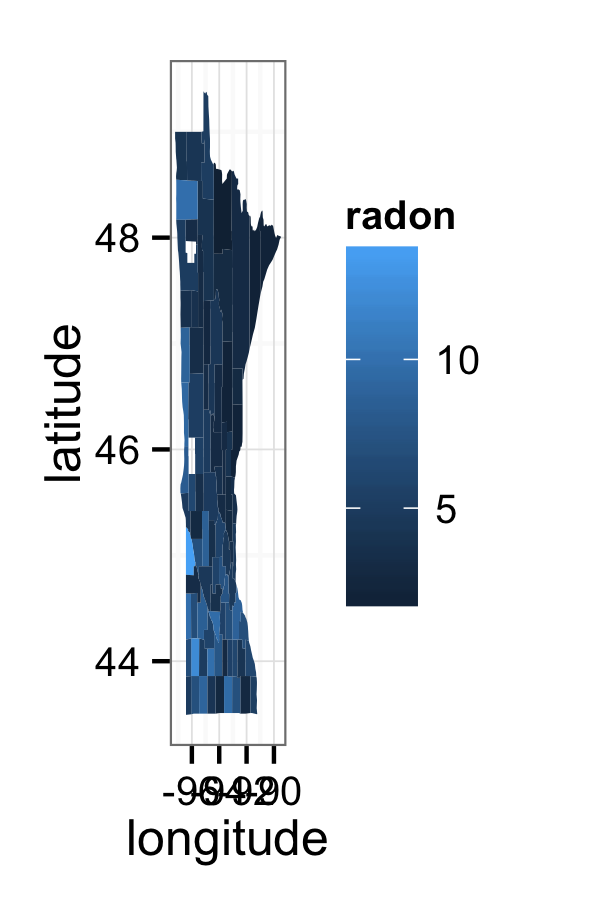
\includegraphics[width=0.45\textwidth]{figures/map.png}
\caption{\label{fig:map} Map of the counties in Minnesota. The color shading represents average radon activity.}
\end{figure}
%
\begin{figure}[htb]
\centering
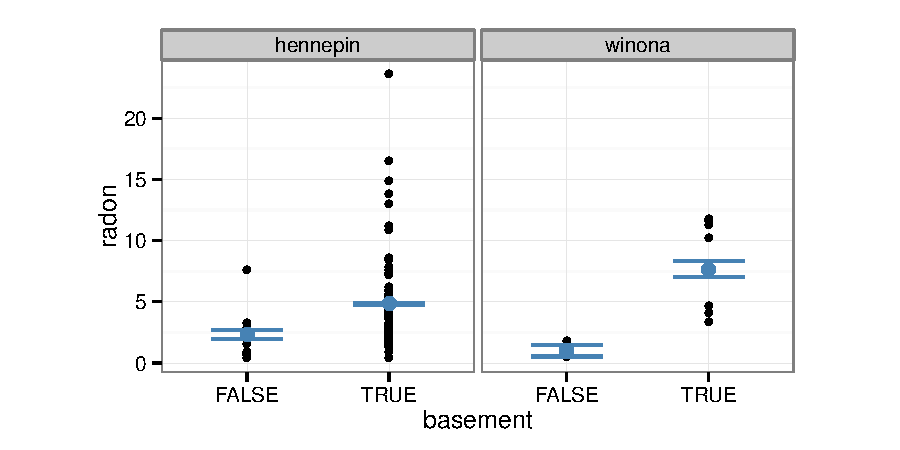
\includegraphics[width=0.7\linewidth]{figures/radon-twocounties.pdf}
\caption{\label{fig:tc} Activity of radon levels for Hennepin and Winona counties at basement (basement = TRUE) or higher in the residence. The bigger points indicate the sample means with 95\% confidence intervals  given by the error bars. Radon levels at the basement level are usually higher.}
\end{figure}
%
The within-county sample sizes, $n_i$, are extremely unbalanced, ranging from one house to 116 houses, with 50\% of the counties having between three and ten houses. Such unbalanced designs are common in applications, and result in a high degree of pooling in the predicted random effects, which results in quantities for many counties that are highly shrunken toward the global mean. It is this high degree of shrinkage that leads to dependence between  predicted random effects and error terms (cf. eqns. \ref{eq:resid1} and \ref{eq:resid2}), which in turn can lead us to draw erroneous conclusions for corresponding residual quantities.

\begin{figure}[!h]
	\centering
	  \subfloat[Predicted error terms]{
		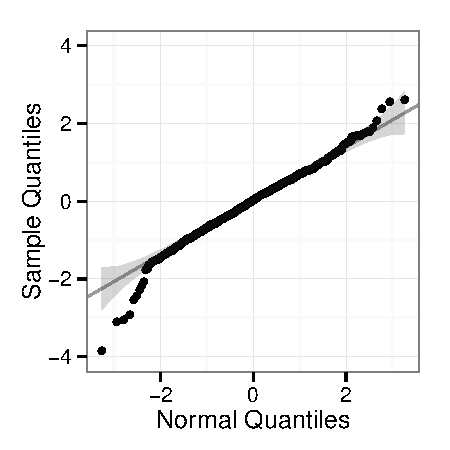
\includegraphics[width=0.33\linewidth]{raw-lev1-qq.pdf}
	   }
	  \subfloat[Random intercepts]{
		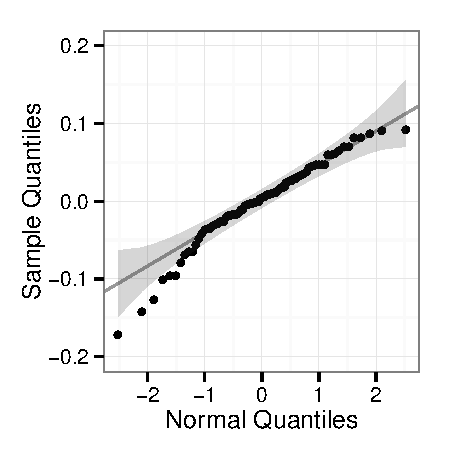
\includegraphics[width=0.33\linewidth]{raw-intercept-qq.pdf}
		}
%	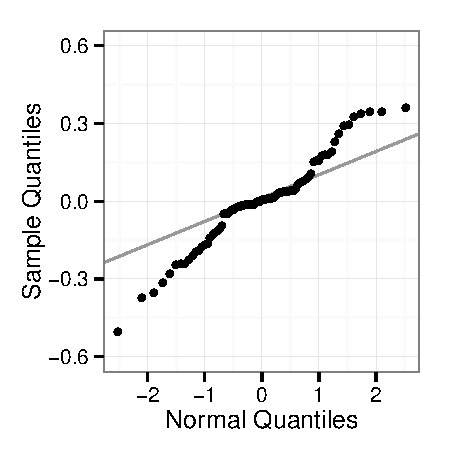
\includegraphics[width=0.32\textwidth]{raw-slope-qq.pdf}
	\caption{\label{fig:qqplots1} Q-Q plots of predicted residuals at different levels %, and random slopes (right) 
	for model~\eqref{eq:radon}. Both plots suggest a deviation of residuals from a normal distribution. Note that random slopes (see figure~\ref{fig:lineup}) exhibit the largest deviation from normality. }
\end{figure}

\begin{figure}[htb]
	\centering
	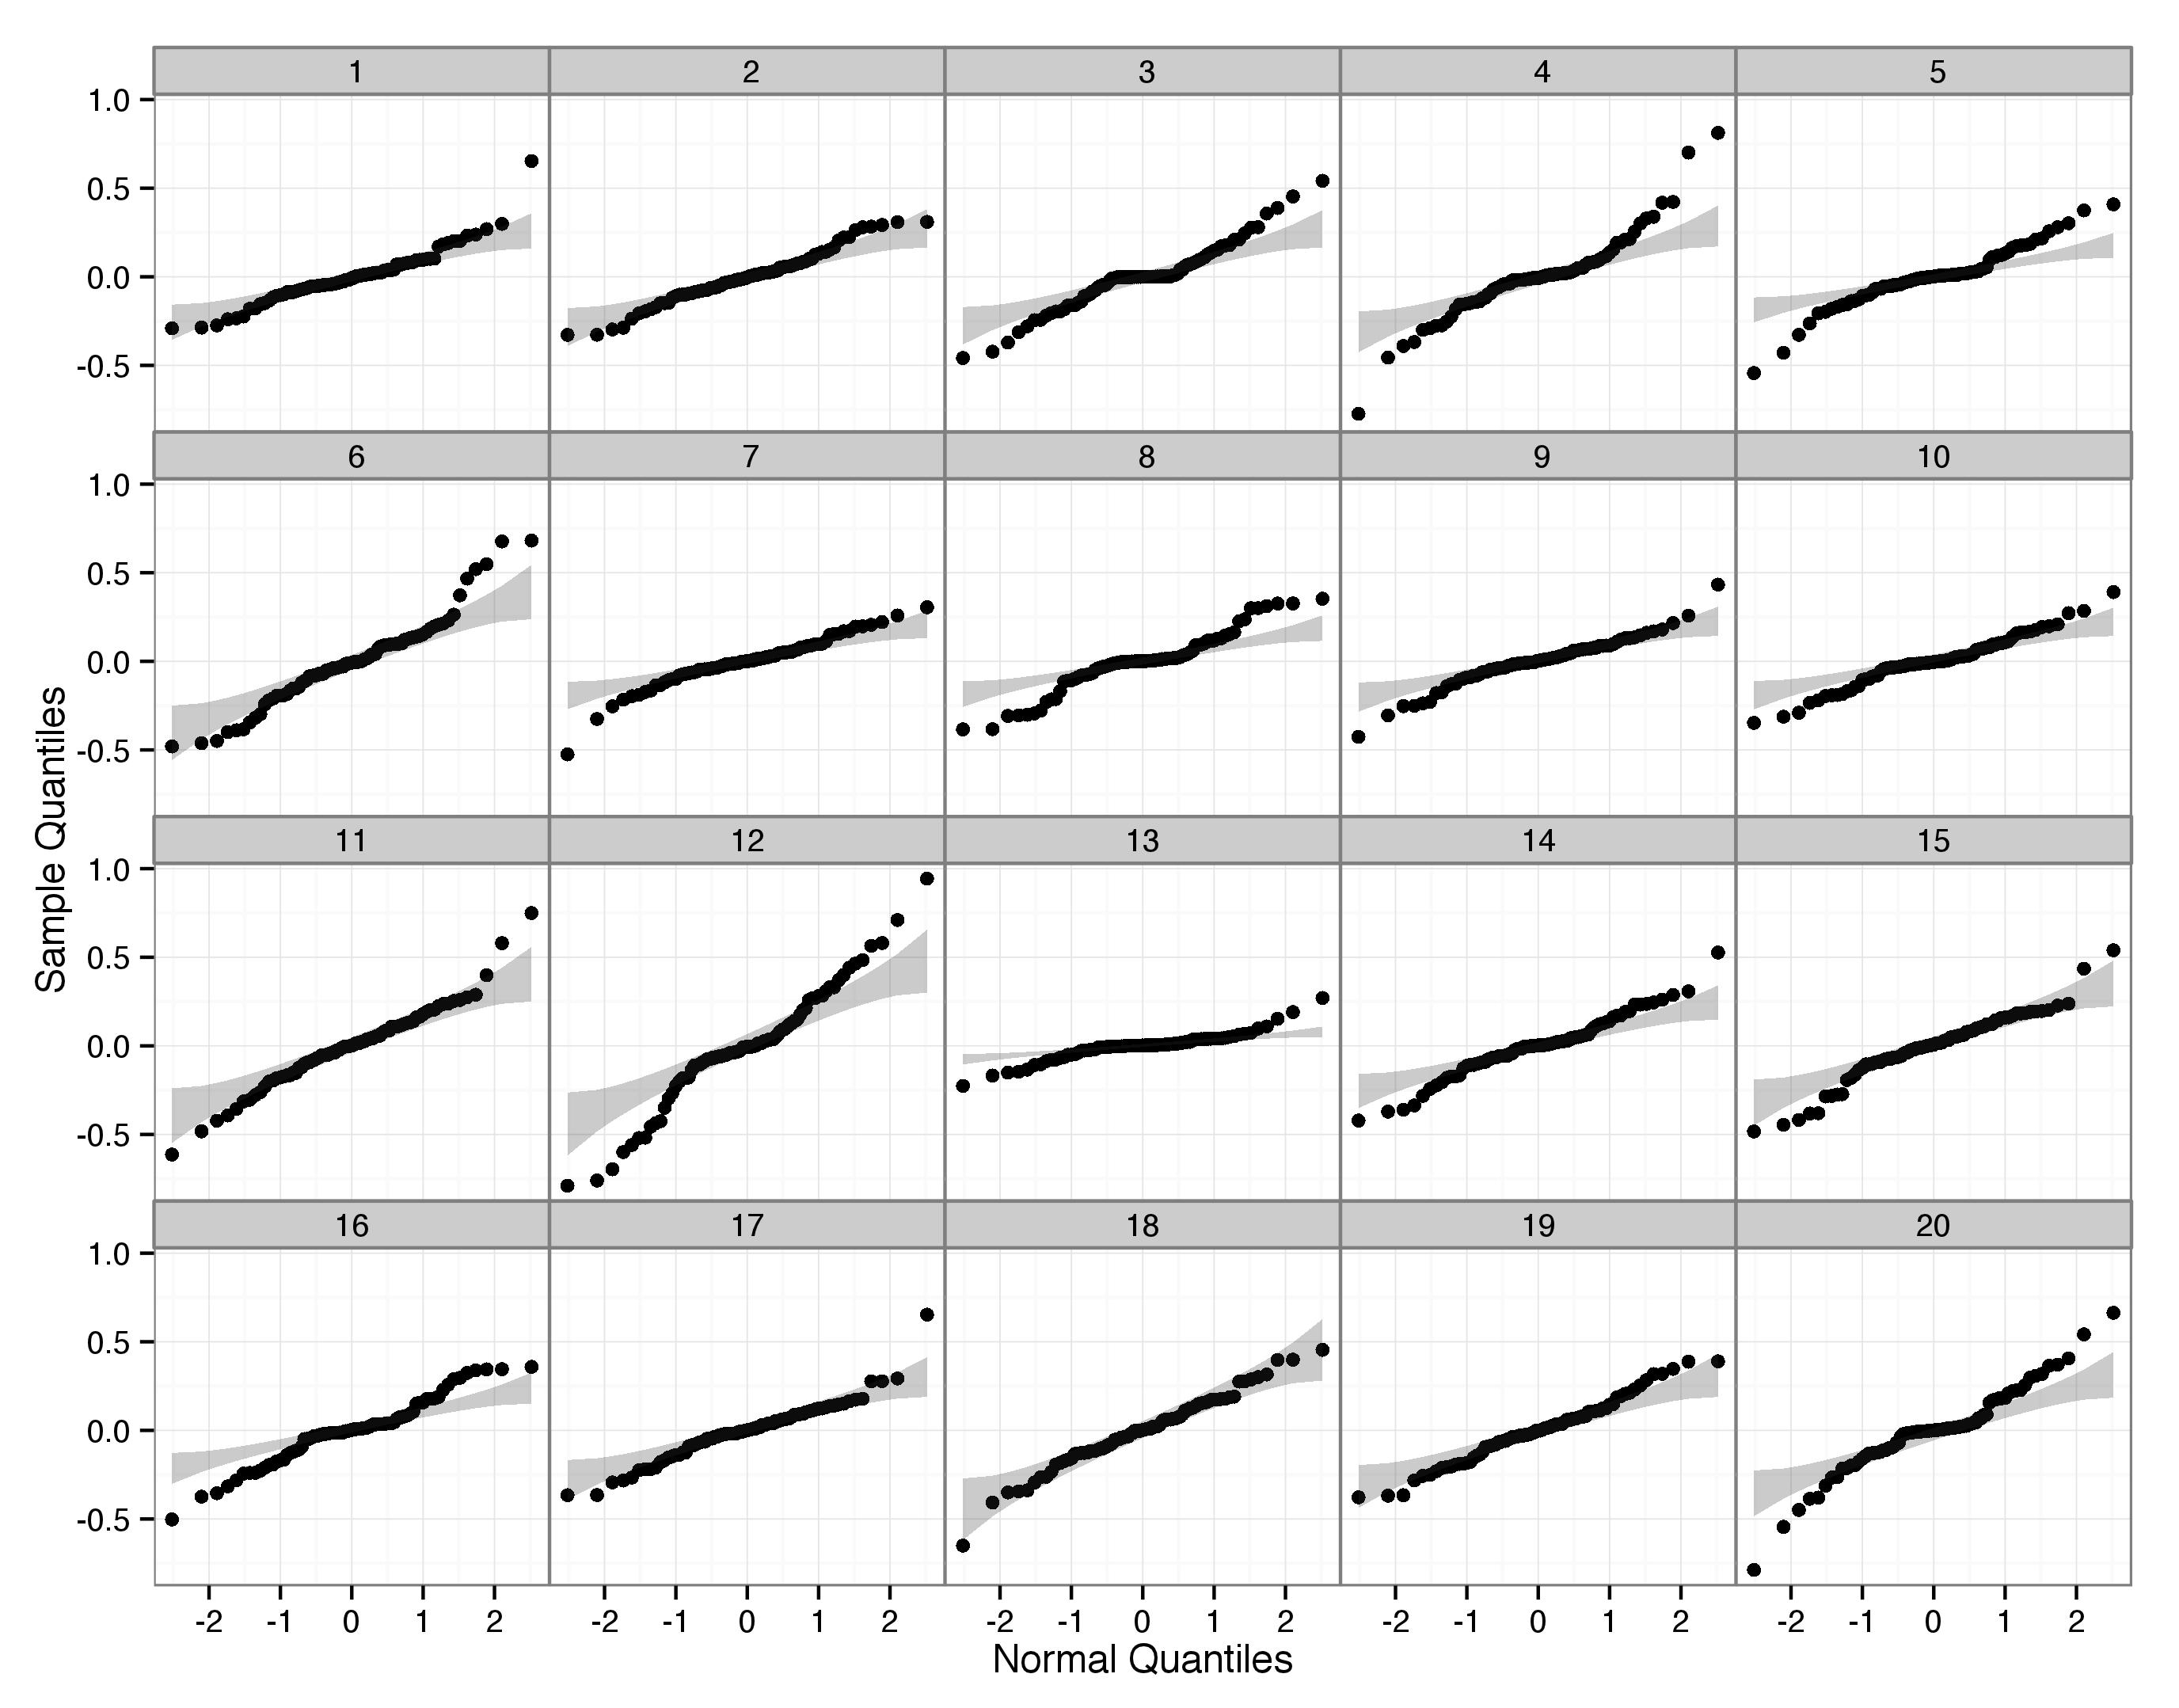
\includegraphics[width=0.9\textwidth]{test.jpeg}%lineup-rslope.pdf}
	\caption{\label{fig:lineup} Lineup of normal Q-Q plots for the random slope term in model~\eqref{eq:radon}. The 19 null plots are obtained by simulation from the model. Can you identify the observed Q-Q plot? }
\end{figure}


In this example, Q-Q plots (Figure~\ref{fig:qqplots1}) for the residuals show that normality 
seems to be violated for the error terms and both random effects. But is this cause for concern?
As there is little pooling at the observation level (level 1) we expect the distributional assessment of the error terms to be reliable, but  the high degree of pooling  for the random effects  casts doubt on the reliability of their Q-Q plots. Next, we assess the reliability of the Q-Q plot for the random slope by utilizing the lineup protocol \citep{buja:2009}:
Figure~\ref{fig:lineup} shows a lineup of 20 Q-Q plots for the predicted random slope. The Q-Q plot of the observed random slopes is placed among 19 decoy plots of parametric bootstrap samples based on model~\eqref{eq:radon} satisfying the normal distribution assumptions. The simulation parameters were set to the maximum likelihood estimates of model~\eqref{eq:radon}. 
If we can identify the real Q-Q plot in the lineup, this provides evidence that the distribution of the observed random slopes is not normal. However, 
the observed Q-Q plot (panel $12+2^2$) is virtually indistinguishable from the field of null plots. This suggests that the predicted random slopes  from the data do not deviate significantly from model~\eqref{eq:radon}. 
%A lineup of the random intercepts revealed the same finding and was omitted for brevity. 
Note that in practice we must blind ourselves from the true plot for proper use of lineups. In order to not violate this, we did not show the Q-Q plot of random slopes earlier.
%
%application of the Anderson-Darling test results in the rejection of the null hypothesis of normality at the .05 significance level for the error terms and both random effects. As there is little pooling at the observation level we would expect the distributional assessment of the error terms to be reliable, but this is not the case with the random effects. 
%
%To further explore the distributional assumptions made on the random effects we create lineups \citep{buja:2009} of quantile plots were created by randomly inserting the true quantile plot for each term into a field of 19 plots generated under the null hypothesis of normality. A lineup for the random slopes is presented in Figure~\ref{fig:lineup}. The observed quantile plot (panel 16) is indistinguishable from the field of null plots, indicating that these predicted random slopes do not deviate from what would be expected under model~\eqref{eq:radon}, contradicting the results of the AD test. 

What becomes apparent from the lineup, is that, astonishingly, {\it none} of the null plots conform to normality. To further investigate the apparent non-normal behavior of predicted random effects we conduct a small simulation study: 
%
We generated 1000 parametric bootstrap samples of model~\eqref{eq:radon} assuming normal random effects and level-1 residuals generated as normal ($\varepsilon_{ij}^* \overset{iid}{\sim}  \mathcal{N}(\bm{0},\ \sigma^2_\varepsilon)$), heavy tailed ($\varepsilon_{ij}^* \overset{iid}{\sim} (\sigma_{\varepsilon} / \sqrt{3})\, t_3$), and skewed ($\varepsilon_{ij}^* \overset{iid}{\sim} \sigma_{\varepsilon} \, \{ \text{Exp}(1) - 1 \}$).
For each simulated data set, we evaluated the assumption of normality for both the level-1 and -2 residuals using the Anderson-Darling (AD), Cram{\'e}r von Mises (CVM) and  Kolmogorov-Smirnov (KS) tests for normality.  
Table~\ref{tab:edf} shows the proportions of these tests rejecting the null hypothesis of normality at the 5\% significance level. 

The type I error rates are hugely inflated for both random effects, making an assessment of normality based on the empirical distribution impossible. 
For example, 84.1\% of the AD tests of the random intercept rejected the null hypothesis of normality when the error terms were skewed.
 Use of standardized random effects and the weighted cumulative distribution function proposed by \cite{Lange:1989uu} reduce the type I errors to the nominal level when the level-1 residuals are normal, but the type I errors remain inflated for non-normal level-1 residuals. 
%Similarly, when the random effects are not normal, simulations (not shown) revealed that the tests were  often unable to reject the null hypothesis of normality when the level-1 residuals were normal. 
Similarly, tests of non-normal random effects often failed to reject if the level-1 residuals were normally distributed. 
This inability to assess distributional assumptions correctly is a symptom typical of confounding between levels of residuals.
%Based on the above results we find that distributional assessment of the predicted random effects is confounded by the distribution of the level-1 residuals.

%The inflated type I error rates for the random effects indicate that the empirical distribution of the random effects cannot be used to assess the assumption of normality. 
In situations with a large amount of pooling, confounding also affects level-1 residuals, which in this particular example were the least affected and did not exhibit signs of deviation from normality.
%In this example we are able to use the empirical distribution to assess normality of  level-1 residuals  as  pooling is minimal at this level. In situations with higher levels of pooling, this may not be the case.

\begin{table}[t]
\centering
\caption{\label{tab:edf} Percentage of tests rejecting the null hypothesis of normality of the predicted random effects at the nominal 5\% significance level when the error terms are normal, heavy tailed, and skewed. The percentages are hugely inflated under each setting compared to the nominal type I error rate. \vspace{.5em}}
\subfloat[Random intercept]{
	\begin{tabular}{l rrr} \hline
	& \multicolumn{3}{c}{Test} \\ \cline{2-4}
	  	&     AD & CVM  & KS \\ \hline
	Normal       	   &	 65.5 & 61.5 &  49.4  \\ 
	Heavy tailed 	   & 89.0 & 87.8 &  78.5  \\ 
	Skewed       	   & 84.1 & 83.0 &  71.5  \\  
	\hline
	\end{tabular}
}
\qquad
\subfloat[Random slope]{
	\begin{tabular}{l rrr} \hline
	& \multicolumn{3}{c}{Test} \\ \cline{2-4}
	  	&     AD & CVM  & KS \\ \hline
	Normal       	  & 87.4 &  86.9 & 81.5  \\ 
	Heavy tailed 	  &	96.5 &	96.7 & 92.7  \\ 
	Skewed       	  &	95.3 &	95.6 & 90.9  \\  
	\hline
	\end{tabular}
}


%\subfloat[Standardized Random intercept]{
%	\begin{tabular}{l rrr} \hline
%	& \multicolumn{3}{c}{Test} \\ \cline{2-4}
%	  	&     AD & CVM  & KS \\ \hline
%	Normal       	   &	 0.048 &	 0.045 &	 0.046  \\ 
%	Heavy tailed 	   & 0.349 & 0.325 & 0.256  \\ 
%	Skewed       	   & 0.520 & 0.487 & 0.399  \\  
%	\hline
%	\end{tabular}
%}
%\qquad
%\subfloat[Standardized Random slope]{
%	\begin{tabular}{l rrr} \hline
%	& \multicolumn{3}{c}{Test} \\ \cline{2-4}
%	  	&     AD & CVM  & KS \\ \hline
%	Normal       	  & 0.039 &	0.041 &	0.048  \\ 
%	Heavy tailed 	  &	0.434 & 0.403 & 0.320  \\ 
%	Skewed       	  &	0.540 & 0.504 & 0.422  \\  
%	\hline
%	\end{tabular}
%}

\end{table}


%\begin{table}[!h]
%\caption{\label{tab:edf} Proportions of tests rejecting the null hypothesis of normality of the predicted error terms and random effects at the nominal .05 significance level. \hh{didn't we want to keep the  background for power? - it should be consistent throughout the paper} Type I error rates are hugely inflated. \vspace{.5em}
%}
%\begin{center}
%\begin{tabular}{l rrr} \hline
%& \multicolumn{3}{c}{Test} \\ \cline{2-4}
% Residual &  AD & CVM & KS \\ \hline
%Error term			 & 0.06 & 0.06 & 0.05\\
%\rowcolor{gray!20} Random intercept 	& 0.48 & 0.46 & 0.35\\
%\rowcolor{gray!20} Random slope 		& 0.75 & 0.75 & 0.68\\
%   \hline
%\end{tabular}
%\end{center}
%\end{table}


In the remainder of this paper we investigate the root of concern that leads to the distributional deviations, and derive residuals that address the issues introduced by pooling, allowing again for a familiar graphical assessment of these distributions.

%----------------------------------------------------------------------------------
\section{Assessing the distribution of the random effects}\label{sec:}
%----------------------------------------------------------------------------------

In this section we develop the rotated random effects and discuss computational and practical issues associated with their use. Before this discussion we present the model and notation used throughout the paper. Additionally, we review the problem of confounding which can be seen in the formulas for the residuals.

%----------------------------------------------------------------------------------
\subsection{Model notation and residuals}\label{sec:resid}
%\subsection{Hierarchical linear models and residuals}\label{sec:resid}
%----------------------------------------------------------------------------------

The general stacked representation of the hierarchical linear model is given by
%
\begin{eqnarray}\label{eq:hlm}
 && \bm{y} = \bm{X \beta} + \bm{Z b} + \bm{\varepsilon}, \\ \nonumber
 && \E \begin{bmatrix} \bm{b} \\ \bm{\varepsilon} \end{bmatrix} = \bm{0}, 
 \ \cov \begin{bmatrix} \bm{b} \\ \bm{\varepsilon} \end{bmatrix} = 
  	\begin{bmatrix} \bm{D} & \bm{0}\\ \bm{0} & \bm{R} \end{bmatrix}
\end{eqnarray}
%
where $\bm{y}$ is an $n \times 1$ vector of observed responses, $\bm{X}$ ($n \times p$) and $\bm{Z}$ ($n \times q$) are design matrices, $\bm{\beta}$ is a $p \times 1$ vector of unknown fixed effects, $\bm{b}$ is a $q \times 1$ vector of unobserved random effects, $\bm{\varepsilon}$ is an $n \times 1$ vector of unobserved errors, and $\bm{R}$ and $\bm{D}$ are positive definite covariance matrices.

  %Additionally, it is often assumed that $\bm{\varepsilon}$ and $\bm{b}$ are normally distributed. 
Using this specification, the predicted error terms and random effects are given by 
%
\begin{align}
\widehat{\bm{\varepsilon}} &= \bm{RPy} = \bm{RPZb} + \bm{RP \varepsilon} \label{eq:resid1}\\
\widehat{\bm{b}} &= \bm{DZ}\trans \bm{Py} = \bm{DZ}\trans \bm{PZb} + \bm{DZ}\trans \bm{P \varepsilon} \label{eq:resid2}
\end{align}
%
where $\bm{P} = \bm{V}\inv( \bm{I} - \bm{X} (\bm{X}\trans \bm{V}\inv \bm{X})\inv \bm{X}\trans \bm{V}\inv)$. This  set of equations %\eqref{eq:resid1} and \eqref{eq:resid2} 
reveals the inherent dependence between the residuals.
Additionally, it is easily seen that both \eqref{eq:resid1} and \eqref{eq:resid2} lead to the analysis of correlated and potentially heteroscedastic disturbances as $\var(\widehat{\bm{\varepsilon}}) = \bm{RPR}$ and $\var(\widehat{\bm{b}}) = \bm{DZ}\trans \bm{PZD}$.
The use of standardized residuals can correct the latter issue, but does not address the fact that the residuals are interrelated. While problems may be expected at both levels of the model based on \eqref{eq:resid1} and \eqref{eq:resid2}, we have found that the interpretation of Q-Q plots of the standardized predicted error terms
%
\[
\bm{z}_{\varepsilon} =  \text{diag} \left(\bm{RPR} \right)^{-1/2} \widehat{\bm{\varepsilon}}
\]
%
is unaffected by this interrelationship. This is not the case with the standardized random effects.  When the degree of pooling is high---as it is in the above radon example, and often is in practice---interpretation of the predicted random effects cannot be separated from the distribution of the error terms. Detailed simulation results documenting the utility of  these residuals are available in the supplementary material.



%----------------------------------------------------------------------------------
\subsection{Rotating the random effects}\label{sec:rotate}
%----------------------------------------------------------------------------------

To combat  confounding between different  levels of residuals, we derive a reduced set of rotated residuals that are standardized, uncorrelated, and homoscedastic. We focus our discussion (and notation) on a two-level model with a single random effect in this section for ease of explanation, and describe how to extend this method at the end of this section.


First, we define the \emph{fraction of confounding} for the random effects, which is minimized in the result below. This definition generalizes the fraction of confounding proposed by \cite{HildenMinton:1995wh}. 

%\begin{definition}[Fraction of confounding]\label{def:fc1}
%For the $i$th element of the target residual vector, $\widehat{\bm{e}}$, the fraction of confounding is given by
%%
%\begin{equation}\label{eq:fc}
%	\text{FC}(\widehat{\bm{e}}_i) 
%	= \frac{\bm{v_i}\trans \var(\widehat{\bm{e}} | \bm{e}) \bm{v_i}}
%		{\bm{v_i}\trans \var(\widehat{\bm{e}}) \bm{v_i}}
%	= \frac{\bm{v_i}\trans \bm{A} \bm{v_i}}
%		{\bm{v_i}\trans \bm{B} \bm{v_i}}
%\end{equation}
%
%where $\bm{v_i}$ is the $i$th column of the identity matrix.
%%\todo[inline]{write this as a minimization problem}
%%This rotation is given by $\bm{M} = \bm{T_r \Lambda_r}^{-1/2} \bm{U}$ where $\bm{T_r \Lambda_r}^{-1/2}$ is the inverse square root of $\bm{B}$ found through the spectral decomposition of $\bm{B}$ and $\bm{U}$ are the eigenvectors of $(\bm{\Lambda_r}^{-1/2} \bm{T_r}\trans) \bm{A} (\bm{\Lambda_r}^{-1/2} \bm{T_r}\trans)\trans$.
%\end{definition}

%Definition~\ref{def:fc1} describes the confounding for each element in the target residual vector individually. An overall measure of the amount of confounding is given below.\\

%\begin{definition}\label{defc:fc2}
%For the target residual vector, $\widehat{\bm{e}}$, the fraction of confounding is given by
%%
%\begin{equation}\label{eq:fc2}
%FC(\widehat{\bm{e}}) = \mathrm{tr}( \var(\widehat{\bm{e}} | \bm{e} ) ) / \mathrm{tr}( \var(\widehat{\bm{e}}) ).
%\end{equation}
%\end{definition}

%\begin{definition}[Fraction of confounding] \hh{define $\bm{b}$ and $\widehat{\bm{b}}$ as well}
%Let $\bm{A} = \var(\widehat{\bm{b}} | \bm{b} )$ and $\bm{B} = \var(\widehat{\bm{b}})$, %which are positive semidefinite matrices by definition. \hh{that doesn't belong in a definition.}
%\al{Also, let $\bm{W}$ be a linear transformation from the original $q$-dimensional space to an $s$-dimensional space ($s \leq q$).} \hh{Where does q come from? } The fraction of confounding in $\widehat{\bm{b}}$ \al{in this $s$-dimensional space} is given by
%%
%\begin{equation}\label{eq:fc2}
%\text{FC}(s; \widehat{\bm{b}}) = \frac{1}{q} \tr\left( \left(\bm{W\trans B W} \right)\ginv \left(\bm{W\trans A W}\right) \right)
%%\dfrac{1}{\ell} \displaystyle{\sum_i} \frac{\bm{v_i}\trans \bm{A} \bm{v_i}}
%%		{\bm{v_i}\trans \bm{B} \bm{v_i}}.
%\end{equation}
%\hh{If FC only depends on s, you imply that for different Ws that have the same rank, you get the same FC. that's not true - so FC needs to be dependent on W. }
%%where $\ell$ is the length of vector $\widehat{\bm{b}}$.
%\end{definition}


\begin{definition}[Fraction of confounding] 
Let $\bm{b}$ denote a vector of $q$ random effects and $\widehat{\bm{b}}$ its predictions as defined in \eqref{eq:resid2}. For a full rank matrix $\bm{W} \in \mathbb{R}^{q \times s}$, where $ s \le q$, the fraction of confounding in the $s$-dimensional space spanned by $\bm{W}$ is defined as 
\begin{equation}\label{eq:fc2}
\text{FC}(\bm{W}; \widehat{\bm{b}}) = \frac{1}{q} \tr\left( \left(\bm{W\trans B W} \right)\ginv \left(\bm{W\trans A W}\right) \right),
%\dfrac{1}{\ell} \displaystyle{\sum_i} \frac{\bm{v_i}\trans \bm{A} \bm{v_i}}
%		{\bm{v_i}\trans \bm{B} \bm{v_i}}.
\end{equation}
where $\bm{B}$ is the covariance structure of $\bm b$, $\bm{B} = \var(\widehat{\bm{b}})$, and $\bm{A}$ is the conditional covariance structure of  $\widehat{\bm{b}}$ given $\bm{b}$,  i.e. $\bm{A} = \var(\widehat{\bm{b}} | \bm{b} )$.
\end{definition}
Note that both $\bm{A}$ and $\bm{B}$ are  positive semidefinite matrices by definition. 


The fraction of confounding measures the contribution of the error terms  to the variance of the random effects. $\text{FC} \in [0,1]$, where 1 indicates that, due to confounding, the predicted random effects contain no information in addition to that found in the error terms, while 0 indicates no confounding. Notice that if $\bm{W}$ is the identity, then \eqref{eq:fc2} measures the fraction of confounding in the original vector of predicted random effects.


In order to correct residuals for the impact of confounding, we propose using the linear transformation of the predicted random effects that substantially reduces the amount of confounding. To do this, we must determine the $s$-dimensional space in which confounding is substantially reduced and find the $\bm{W}$ that minimizes confounding within that space. To determine the dimension of the subspace spanned by the rotated residuals we propose the use of a  visual tool similar to the scree plots used for selecting the number of principal components. The construction of such plots depends on the linear transformation $\bm W$, so we first discuss the selection of $\bm{W}$ \hh{given  a fixed dimension $s$.}

\paragraph{Selecting the optimal linear transformation.}
For a given $s$-dimensional space, the linear combination $\bm{W} \in \mathbb{R}^{q \times s}$ that minimizes \eqref{eq:fc2} also minimizes
%
\begin{equation}\label{eq:minimize}
J_1(s) = \tr\left( \left(\bm{W\trans B W} \right)\inv \left(\bm{W\trans A W}\right) \right)
%\displaystyle{\sum_i} \frac{\bm{v_i}\trans \bm{W} \bm{A} \bm{W}\trans \bm{v_i}}
%		{\bm{v_i}\trans \bm{W} \bm{B} \bm{W}\trans \bm{v_i}}
\end{equation}
%
Mathematically, this problem is solved using the generalized eigenvalue decomposition
%
\begin{equation}\label{eq:geigen}
	\bm{Aw}_k = \gamma_k \bm{Bw}_k
\end{equation}
%
where $\gamma_k$ and $\bm{w}_k$ are the $k$-th smallest eigenvalues and eigenvectors, respectively \citep{Fukunaga:1990}. 
%thus, $\bm{W}^*$ consists of the eigenvectors associated with the $s$ smallest eigenvalues. 
Computationally, we solve this problem by simultaneous diagonalization of $\bm{A}$ and $\bm{B}$ \citep{McDonald:1979ca, deLeeuw:1982to}. Simultaneous diagonalization of $\bm{A}$ and $\bm{B}$ requires $\bm{W}$ to be $\bm{B}$-orthogonal, so the optimal $\bm{W}$ is found to be
%
\begin{equation}\label{eq:optimw}
	\bm{W}^*(s) = \argmin_{ 
%\begin{scriptsize}
%	\begin{cases}
      \bm{W} \in \mathbb{R}^{q \times s}, \ \ 
      \bm{W\trans B W} = \bm{I}
%	\end{cases}
%\end{scriptsize}
	} 
\tr\left( \bm{W\trans A W} \right) 
\end{equation}
%
Below, we outline the procedure used to simultaneously diagonalize $\bm{A}$ and $\bm{B}$ for reference.\\
%and refer the reader to \cite{McDonald:1979ca} and \cite{deLeeuw:1982to} for additional details on simultaneous diagonalization of two positive semidefinite matrices.\\

\begin{algorithm}[Simultaneous diagonalization]
Let $\bm{A}$ and $\bm{B}$ be two positive semidefinite matrices. The transformation that simultaneously diagonalizes both matrices can be found through the following procedure:
\begin{enumerate}
\item Find a transformation that whitens $\bm{B}$. Such a transformation is given by $\bm{T_r \Lambda_r}^{-1/2}$, where $\bm{T}_r$ and $\bm{\Lambda}_r$ are the first $r$  eigenvectors and eigenvalues of $\bm{B}$, where $r = \rank(\bm{B})$. 

\item Transform $\bm{A}$ and $\bm{B}$ to
\begin{align}
\bm{\Lambda_r}^{-1/2} \bm{T_r}\trans \bm{A T_r \Lambda_r}^{-1/2} &= \bm{A}^* \label{eq:astar} \\
\bm{\Lambda_r}^{-1/2} \bm{T_r}\trans \bm{B T_r \Lambda_r}^{-1/2} &= \bm{I}
\end{align}

\item Find an orthonormal transformation that diagonalizes $\bm{A}^*$. Such a transformation is given by the eigenvectors of $\bm{A}^*$, which we denote $\bm{U}$.
\end{enumerate}

Based on the above three steps, the transformation that simultaneously diagonalizes $\bm{A}$ and $\bm{B}$ is $\bm{T_r \Lambda_r}^{-1/2} \bm{U}$.\\ 
\end{algorithm}

The above procedure can be used to find the general solution to \eqref{eq:geigen}. To find the more specific transformation defined by \eqref{eq:optimw}, we focus on the $s$ eigenvectors associated with $s$ the smallest eigenvalues of $\bm{A}^*$, $\bm{U}_s$, making
%
\begin{equation}\label{eq:w}
\bm{W}^* = \bm{T_r \Lambda_r}^{-1/2} \bm{U}_s
\end{equation}
%
The rotated random effects are then given by $\bm{W}^{*\prime} \widehat{\bm{b}}$, which are standardized, uncorrelated, and homoscedastic (see the appendix for a proof).

%\todo[inline]{Address that the order of the data will influence the resulting residuals.}
%Since $\bm{B}$ is only positive semidefinite, it is important to note that the order of the groups in the data change the resulting residuals. In this case, the transformation in \eqref{eq:astar} eliminates a group


%Having considered the computational aspects of the problem we must next consider the more practical aspects. 

%\al{Having considered the optimal linear transformation for a given $s$-dimensional subspace, we return to the problem of selecting the dimension which substantially reduces the fraction of confounding.}


\paragraph{Selecting the dimension of the subspace.}
Selection of the dimension of the subspace spanned by the rotated residuals is central to our proposed method. Ideally, we would select the dimension such that the fraction of confounding is reduced to zero; however, this is not realistic in practice. Alternatively, we propose choosing the dimension that provides a substantial reduction in the fraction of confounding. Since our ultimate objective is distributional assessment, we must balance this reduction in the fraction of confounding with the loss in power of a test of the empirical distribution function (e.g., the Anderson-Darling test for normality) associated with dimension reduction. To guide this choice we suggest plotting the reduction in the fraction of confounding against the reduction in dimension, which is similar to the scree plot used to select the number of principal components. To illustrate the use of this plot we simulate two simple random intercept models with a group-level predictor:   model $M1$ has 40 groups of 30 observations and 10 groups of 5 observations;   model $M2$ also has 50 groups, with group sizes determined as random draws from either a Poisson(30) distribution (40 groups) or a Poisson(5) distribution (10 groups). \todo[inline]{These two models are very similar. Go to a more extreme in the second model?}
 Figure~\ref{fig:elbow} shows two examples of such plots constructed for the simulated models. Both figures have an ``elbow'' in the plot corresponding to a reduction in the dimension of the subspace of 11; thus we would choose $s = 39$.
%
\begin{figure}[htb]
	\centering
	 \subfloat[Model $M1$]{
		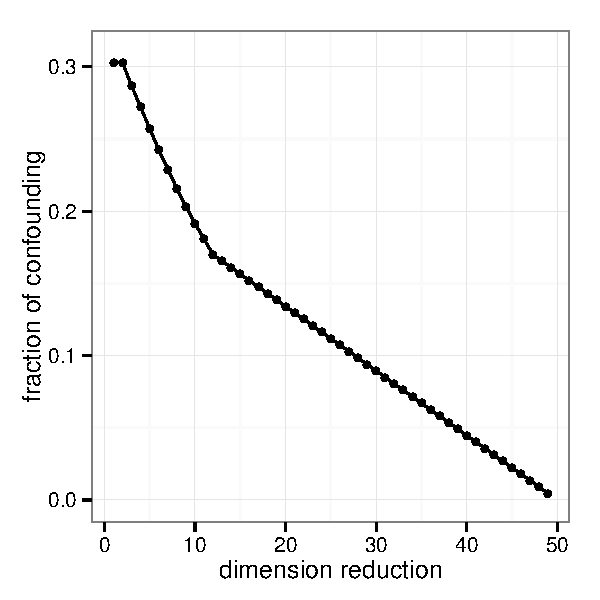
\includegraphics[width=0.4\linewidth]{elbow1.pdf}
		}
	  \subfloat[Model $M2$]{
		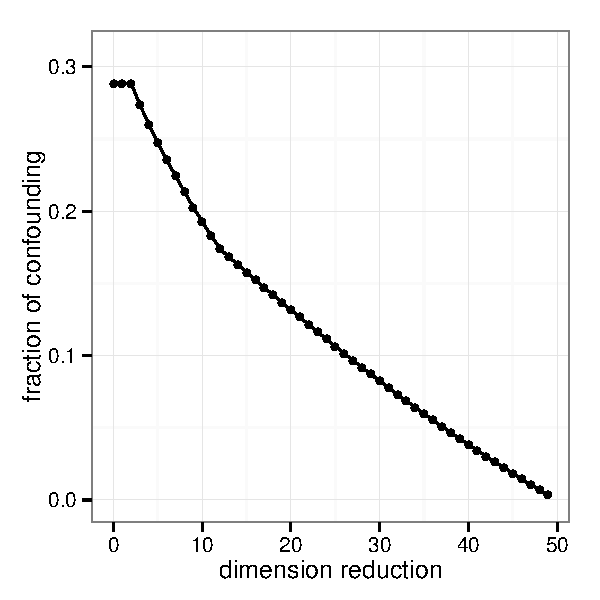
\includegraphics[width=0.4\linewidth]{elbow2.pdf}
		}	
	\caption{\label{fig:elbow} Plots of the fraction of confounding for each reduction in the dimension of subspace spanned by the rotated random intercepts from two simulation models. Model $M1$ has 50 groups: 40 groups of size 30, and 10 groups of size 5. Model $M2$ has 50 groups with group sizes determined as random draws from either a Poisson(30) distribution (40 groups) or a Poisson(5) distribution (10 groups). Based on these plots we  choose $s = 39$, corresponding to a dimension reduction of 11.}
\end{figure}


%%First, we must consider the selection of the dimension of the subspace spanned by the rotated residuals, $s$---that is, the length of the resulting transformed residual vector. 
%For the level-1 residuals \cite{HildenMinton:1995wh} suggests using $s = \rank(\bm{B})$;
%%One choice is $s = \rank(\bm{B})$, which aligns with the suggestion given by \cite{HildenMinton:1995wh} for the level-1 residuals. 
%%This selection has the advantage that it works in all situations, but the disadvantage that the fraction of confounding will \al{often} not be \al{significantly} reduced. 
%An alternative approach is to select $s$ based on the desired reduction in the fraction of confounding. \hh{You need to sell this point a bit more - what is the theoretical advantage of going down on the number of residuals? -- if the approach is to get FC down as much as possible, but have s at least 30, it is always going to end up at 30. What I still don't understand is that the minimization is not taking care of the percent of confounding to a higher degree, because that's really what it was supposed to do. }
%%A starting point for this approach can be determined for a given reduction in the fraction of confounding by considering the relative contributions of the ordered diagonal elements of $\bm{B}\ginv\bm{A}$ to \eqref{eq:fc2}. 
%We consider this approach in the simulation study presented in Section~\ref{sec:simulation} and present the results in Figure~\ref{fig:fc}. Note that in some situations it will not be possible to reduce the fraction of confounding much as the number of groups limits this reduction.

\paragraph{Correcting for supernormality.}
The transformation of the random effects results in a vector where each component is a linear combination of elements of $\widehat{\bm{b}}$. Consequently, the rotated residuals will appear more normal than the underlying distribution, if the underlying distribution is not normal. This issue is often referred to as supernormality \citep{Atkinson:1985}. One approach to address supernormality in this context is to reduce the number of elements in the linear combinations, which should reduce the extent of the problem. To do this, we suggest using an orthogonal rotation of $\bm{W}^*$, which we denote $\bm{Q}$, just as we rotate the factor loadings in factor analysis. Using this approach, the rotated residuals are obtained by $\bm{Q}\trans \bm{W}^{*\prime} \widehat{\bm{b}}$. One rotation that will produce rotated residuals comprised of a small number of raw residuals is the raw varimax rotation \citep{Johnson:2007}. Figure~\ref{fig:cartoon} displays heatmaps of $\bm{W}^{*\prime}$ (left) and $\bm{Q}\trans\bm{W}^{*\prime}$ (right) for a simulated random intercept model with 20 groups, and demonstrates that the raw varimax rotation reduces the number of groups loading highly on each rotated residual. %\hh{what amount of confounding is there on the left and then on the right?} \al{The amount of confounding is the same between the right and the left. The only different between the two is that we applied the varimax transform to the plot on the right. Regardless, $FC \approx .25$. I used this small simulated model because I thought it showed what the varimax can do for us.} 
Other orthogonal rotations could be used, but the varimax rotation is familiar to a wide range of analysts and is widely implemented in statistical software packages. A similar approach was used by \cite{Jensen:1999iu}, who used the raw varimax rotation to produce recovered errors for distributional assessment in the ordinary regression model.

\begin{figure}[t]
	\centering
	\subfloat[$\bm{W}^{*\prime}$]{
		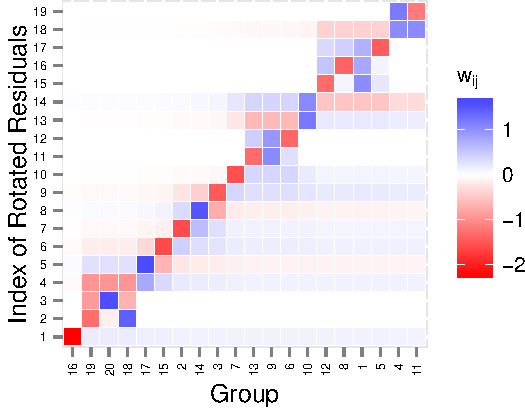
\includegraphics[width=0.4\textwidth]{cropped_cartoon_heatmap_raw.pdf}
	}
	\qquad
	\subfloat[$\bm{Q}\trans\bm{W}^{*\prime}$]{
		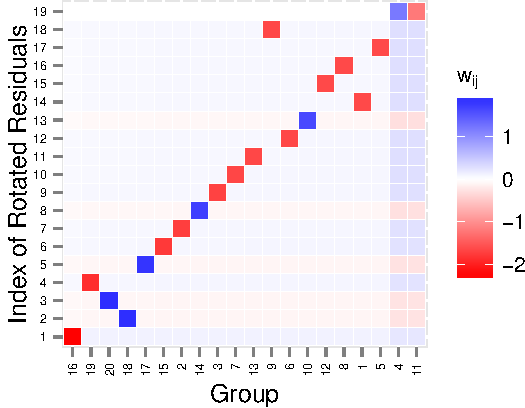
\includegraphics[width=0.4\textwidth]{cropped_cartoon_heatmap_varimax.pdf}
	}
	\caption{\label{fig:cartoon} Heatmap of $\bm{W}^{*\prime}$ and $\bm{Q}\trans\bm{W}^{*\prime}$ calculated where $\bm{Q}$ for a simulated random intercept model with 20 groups. Applying the raw varimax rotation, $\bm{Q}$, reduces the number of groups loading on a given rotated residual.}
\end{figure}

\paragraph{Extension to multiple random effects.}
Up to this point our discussion has ignored that a model may (and often will) contain numerous random effects. In this case, the assumptions made on each random effect should be checked; thus, we propose assessing each random effect separately. To this end we must define linear combinations $\bm{L}_k$ such that $\bm{L}_k\trans \widehat{\bm{b}}$ produces the $k$th marginal random effect. For example, in a model with a random intercept and random slope, if $\bm{Z}$ is organized as a block diagonal matrix---that is $\bm{Z} = \bigoplus_{i=1}^{m} \bm{Z}_{i}$ where $\bigoplus$ denotes the direct sum \citep[page 47]{Gentle:2007}---then $\bm{L}_0 = \bm{I}_{m} \bigotimes ( 1,\ 0)$ produces the random intercepts and $\bm{L}_1 = \bm{I}_{m} \bigotimes ( 0,\ 1)$ produces the random slopes. The methodology presented in this section can be generalized to models with numerous random effects by substituting $\bm{L}_k\trans \widehat{\bm{b}}$ for $\widehat{\bm{b}}$.


%----------------------------------------------------------------------------------
\section{Simulation study}\label{sec:simulation}
%----------------------------------------------------------------------------------

We conducted a simulation study to assess the specificity and sensitivity of tests of normality based on the two rotated residuals proposed in the previous section. 

\subsection{Design}\label{sec:sim-design}
%----------------------------------------------------------------------------------

We want to examine situations in which we correctly and incorrectly reject the null hypothesis of normality---that is, power and type I error, respectively. We compute the proportion of Anderson-Darling (AD), Cram{\'e}r von Mises (CVM), and Kolmogorov-Smirnov (KS) tests that rejected the null hypothesis of normality.
 These test statistics each measure the discrepancy between the empirical distribution of the rotated random effects and assumed distribution of the random effects, which sheds light on the behavior of Q-Q plots constructed from the rotated residuals. 


The design matrices from model \eqref{eq:radon} were used as templates for realistic data generation;  for simplicity of the simulation design, only the 60 counties with full rank $\bm{Z}$ matrices were included. 
Normal, heavy-tailed, and skewed distributions are used to generate the simulated errors and random effects. We use a rescaled $t$ distribution with 3 degrees of freedom to generate heavy tailed residuals, and a centered and rescaled exponential distribution with a rate parameter of 1 to generate skewed residuals. For simplicity we require the distributions of the random slope and intercept to the be same and assume independence between the random effects. The 9 distributional settings considered in the simulation study are summarized in Table~\ref{tab:simdsns}.

\begin{table}[htdp]
\centering
\caption{\label{tab:simdsns} A summary of the 9 distributional settings considered in the simulation study.}
\begin{tabular}{llccc}\hline
Distributions of & & \multicolumn{3}{c}{Random effects, $F_2$} \\ \cline{3-5}
           & & $\mathcal{N}(0, \ \sigma^2_{b})$ & $(\sigma_{b} / \sqrt{3})\, t_3$ & $\sigma_{b} \, \{ \text{Exp}(1) - 1 \}$ \\ \hline
Error terms, $F_1$  & $\mathcal{N}(0, \ \sigma^2_{\varepsilon})$       & &&\\
             & $(\sigma_{\varepsilon} / \sqrt{3})\, t_3$  &  & $\varepsilon_{ij}^* \overset{iid}{\sim} F_1, \ \ b_{0i}^*, b_{1i}^* \overset{iid}{\sim} F_2$ &  \\
             & $\sigma_{\varepsilon} \, \{ \text{Exp}(1) - 1 \}$       & && \\ 
\hline
\end{tabular} 
\end{table}

Additionally, the the fixed effects coefficients were set to the maximum likelihood estimates.

To investigate the effect that pooling has on the rotated random effects we considered  three variance structures to represent different degrees of confounding for the random effects:\\
%
\begin{tabular}{ll}
\textbf{high:} & $\sigma^2_\varepsilon = 4$ and  $\sigma^2_{b_0} = \sigma^2_{b_1} = 1$ \\
\textbf{moderate:} & $\sigma^2_\varepsilon = 1$ and  $\sigma^2_{b_0} = \sigma^2_{b_1} = 1$ \\
\textbf{low:} & $\sigma^2_\varepsilon = 1$ and  $\sigma^2_{b_0} = \sigma^2_{b_1} = 4$ \\
\end{tabular}
%

Under each simulation setting 1000 data sets were generated for each model and the rotated residuals were obtained using $s = \rank(\bm{B})$ (which is 58 and 59 for the random intercept and slope, respectively) as well as $s =$ 55, 50, 45, 40, 35, and 30.


\subsection{Results}\label{sec:sim-results}
%----------------------------------------------------------------------------------

Figure~\ref{fig:fc} shows the average fraction of confounding for the rotated random intercept (left) and random slope (right) over the different values for $s$ for each variance structure. As $s$ is reduced, the fraction of confounding is reduced, which aligns with expectation as smaller choices of $s$ reduce the contributions of more highly confounded groups.

\begin{figure}[h]
	\centering
	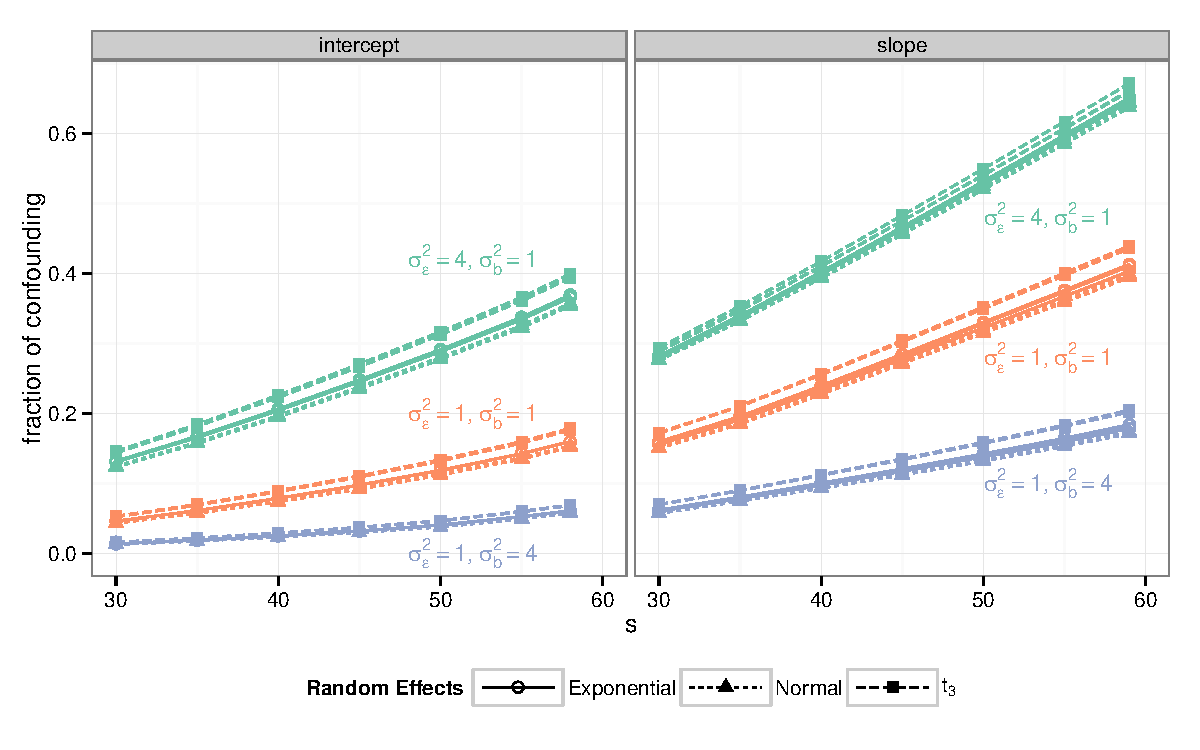
\includegraphics[width=\textwidth]{fc_by_s.pdf}
	\caption{\label{fig:fc} Change in the fraction of confounding (FC) as the dimension of the rotated random effects vector, $s$, is reduced for the three variance structures considered in the simulation study. %LOESS smoothers estimate the trajectory of FC as $s$ varies.} 
	}
\end{figure}

\al{Table~\ref{tab:results-int} and Figure~\ref{fig:results-slope}} display the estimated type I error rates using the AD normality test ($\alpha = 0.05$) on the rotated and varimax rotated random intercepts and random slopes, \al{respectively}, when $\sigma^2_\varepsilon = 4$ and $\sigma^2_{b_0} = \sigma^2_{b_1} = 1$. The CVM and KS tests performed similarly and are omitted for brevity (full simulation results can be found in the supplementary material). Both figures show that the type I error rate is stabilized close to the nominal level with the appropriate choice of $s$. For the random intercept most choices of $s$ perform reasonably well, with the type I error rate closest to the nominal level for all error distributions between 30 and 40. For the random slope, $s$ must be chosen to be 30 for type I error to be near the nominal level; however, $s$ may need to be even smaller to achieve the nominal rate. 


%\begin{figure}
%	\centering
%	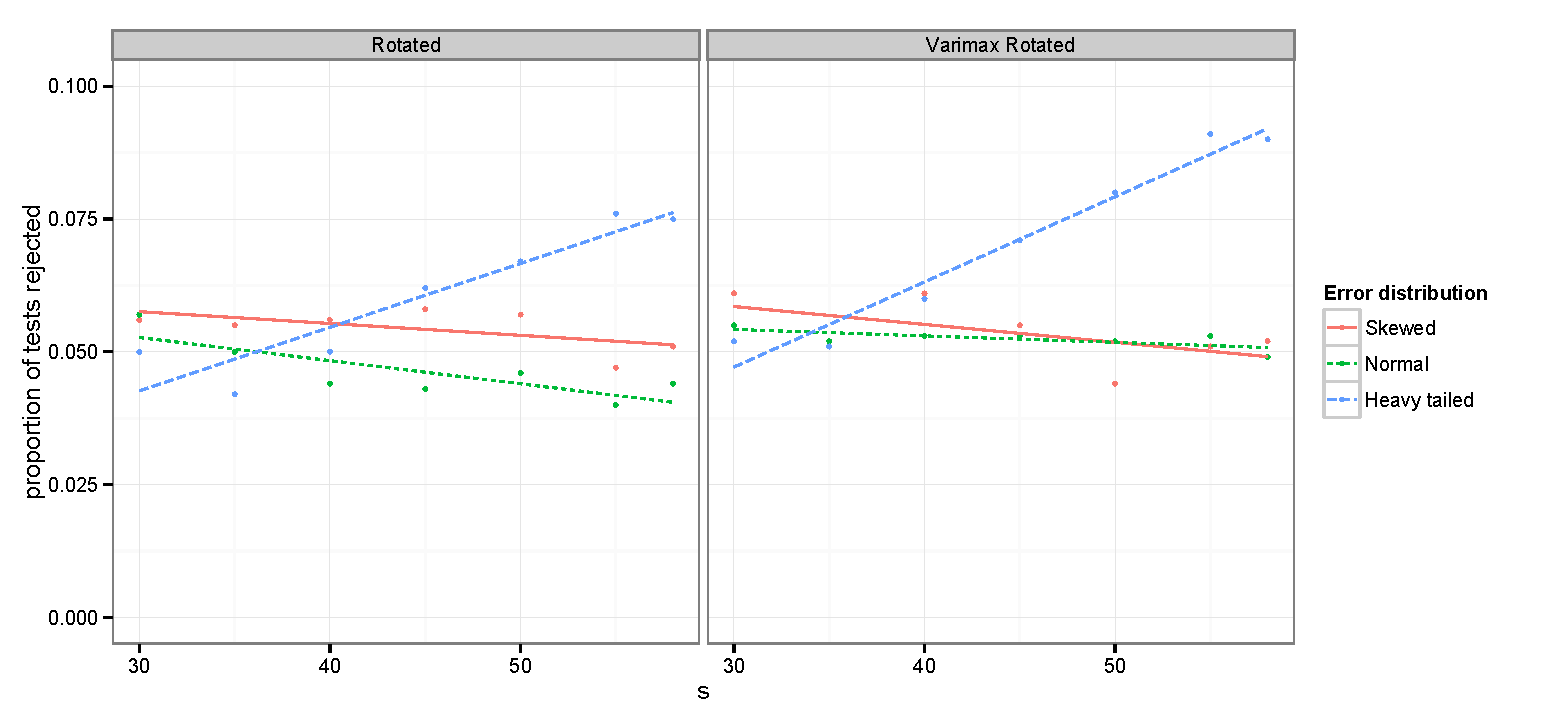
\includegraphics[width=\textwidth]{ad_intercept_results.pdf}
%	\caption{\label{fig:results-int} Estimated type I error rate using the Anderson-Darling normality test ($\alpha = 0.05$) on the rotated random intercepts (left) and varimax rotated random intercepts (right) by the distribution of the error terms and $s$. }
%\end{figure}

\begin{figure}
	\centering
	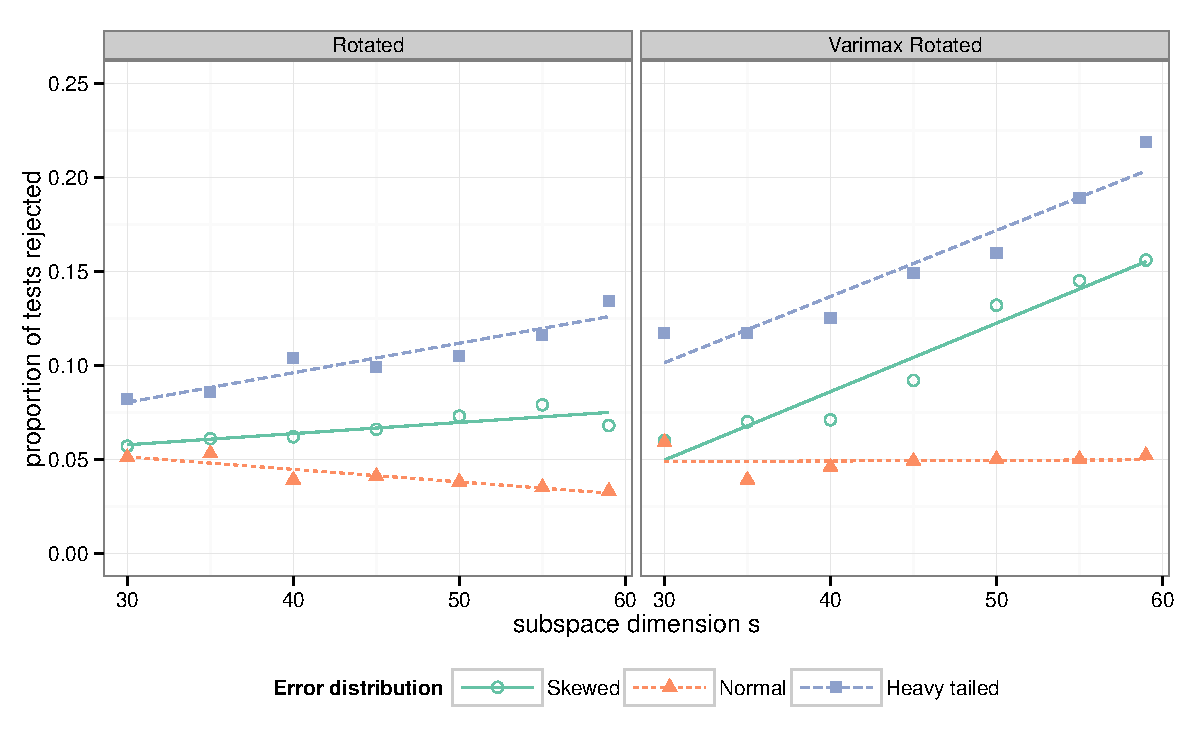
\includegraphics[width=0.9\textwidth]{ad_slope_results.pdf}
	\caption{\label{fig:results-slope} Estimated type I error rate using the Anderson-Darling normality test ($\alpha = 0.05$) on the rotated random slopes (left) and varimax rotated random slopes (right) by the distribution of the error terms and $s$.}
\end{figure}

\al{Table~\ref{tab:results-int}  and Figure~\ref{fig:power-slope}} show the estimated power of the AD test ($\alpha = 0.05$) on the rotated and varimax rotated random intercepts and random slopes, respectively, for the highly confounded variance structure. The estimated power to detect non-normal random effects distributions is amplified by the varimax rotation and larger choices of $s$. We also find that the estimated power is lower than would be expected from randomly sampled values from an exponential or $t_3$ distribution (what we will refer to as the ``gold standard''). 
%\hh{the gold standard should show in your figures as well, so that we have a way of gauging the loss in power other than perfect power of 1, which is going to make any gain in power look small.} 
%\al{I can do this, but the power for detecting the exponential at these sample sizes is very high, which makes things look small. The AD test has less power to detect the t distribution at these sample sizes.}
For example, when $s=30$, simulations indicate the power of the AD test to detect a $t_3$ distribution to be approximately 0.4, whereas our simulations indicate nearly half the power, with the random slope generally having lower power than the random intercept. Interestingly,  there is higher power to detect a heavy tailed distribution than a skewed distribution.  Additional simulations (not discussed) using a model with a continuous variable defining the random slope showed results similar to the random intercept(Table~\ref{tab:results-int}).


While the estimated power is lower than the gold standard, the fact that the type I error rate can be stabilized indicates that distributional problems detected using the rotated random effects will truly be problems; thus, providing more diagnostic information than the (unrotated) predicted random effects.


\begin{figure}
	\centering
	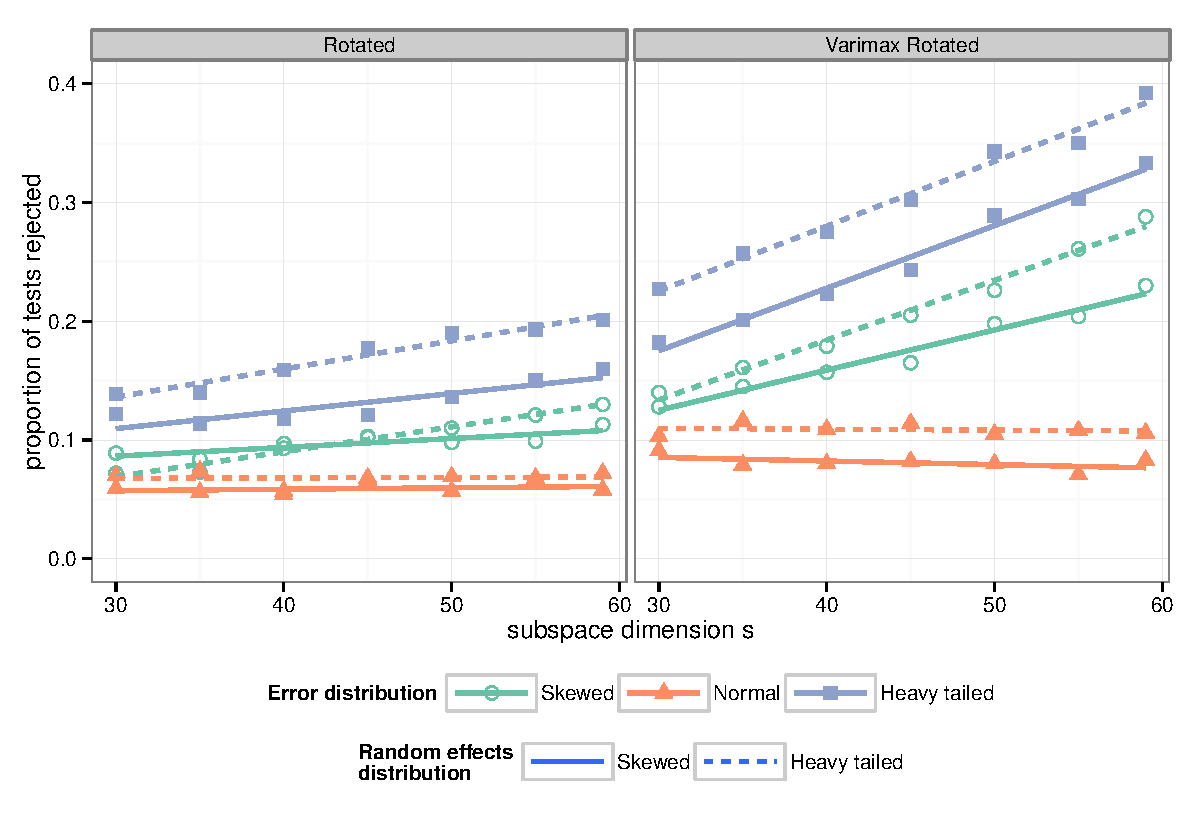
\includegraphics[width=0.9\textwidth]{ad_slope_power.pdf}
	\caption{\label{fig:power-slope}Linear smoother of the estimated power using the Anderson-Darling normality test ($\alpha = 0.05$) on the rotated random slopes (left) and varimax rotated random slopes (right) by $s$. The color denotes the distribution of the errors and the line type denotes the distribution of the random slope.}
\end{figure}


\begin{table}
\centering
\caption{\label{tab:results-int} Percentages of AD tests rejecting the null hypothesis of normality at the 5\% significance level for the rotated (a) and varimax rotated (b) random intercepts by $s$. The gray shading indicates the situations where the random intercept is normal (i.e., type I error).}
\subfloat[Rotated random intercept.]{
	\begin{tabular}{ll rrrrrrr} \hline
	& & \multicolumn{7}{c}{$s$} \\ \cline{3-9}
	Random intercept & Error term & 58 & 55 & 50 & 45 & 40 & 35 & 30\\ \hline 
\rowcolor{gray!20}Normal	&	Normal			& 4.4	& 	4.0	& 4.6	& 4.3	&	4.4	&	5.0	&	5.7 \\
\rowcolor{gray!20}	    &	Heavy tailed		& 7.5	&	7.6	& 6.7	& 6.2	&	5.0	&	4.2	&	5.0 \\	
\rowcolor{gray!20}	    &	Skewed			& 5.1	&	4.7	& 5.7	& 5.8	&	5.6	&	5.5	&	5.6 \\	
&&&&&&&&\\
Heavy tailed	&	Normal		& 13.9	&	13.6	& 13.1	& 13.4	&	13.0	&	13.1	&	12.1 \\	
	        & Heavy tailed	& 19.0	&	18.6	& 16.7	& 16.1	&	16.0	&	14.8	&	13.9 \\	
			& Skewed			& 15.5	&	15.1	& 14.2	& 13.6	&	13.2	&	12.7	&	11.9 \\
&&&&&&&&\\
Skewed	&	Normal			& 9.6	&	8.7	& 9.5	& 9.7	&	10.0	&	11.0	&	10.0 \\	
		&	Heavy tailed		& 12.6	&	12.5	& 12.0	& 11.3	&	10.1	&	11.3	&	11.0 \\	
		&	Skewed			& 13.4	&	13.4	& 12.2	& 12.2	&	11.0	&	11.3	&	10.8 \\
\hline
	\end{tabular}
}

\subfloat[Varimax rotated random intercept.]{
	\begin{tabular}{ll rrrrrrr} \hline
	& & \multicolumn{7}{c}{$s$} \\ \cline{3-9}
	Random intercept & Error term &  58 & 55 & 50 & 45 & 40 & 35 & 30\\ \hline
\rowcolor{gray!20}Normal	&	Normal			& 	4.9	& 	5.3	&	5.2	&	5.3	&	5.3	&	5.2	&	5.5	\\
\rowcolor{gray!20}	    &	Heavy tailed		& 	9.0	&	9.1	&	8.0	&	7.1	&	6.0	&	5.1	&	5.2	\\
\rowcolor{gray!20}	    &	Skewed			& 	5.2	&	5.1	&	4.4	&	5.5	&	6.1	&	5.1	&	6.1	\\
&&&&&&&&\\
Heavy tailed	&	Normal		& 	22.1	&	22.3	&	23.3	&	22.9	&	23.3	&	22.3	&	21.6	\\
	        & Heavy tailed	& 	34.4	&	33.3	&	32.1	&	31.6	&	30.1	&	27.0	&	26.6	\\
			& Skewed			& 	27.8	&	26.7	&	25.6	&	27.0	&	24.4	&	23.1	&	21.8	\\
&&&&&&&&\\
Skewed	&	Normal			& 	19.7	&	21.2	&	21.3	&	22.1	&	22.7	&	21.1	&	22.3	\\
		&	Heavy tailed		& 	29.7	&	28.4	&	27.1	&	25.0	&	25.5	&	25.0	&	23.8	\\
		&	Skewed			& 	22.2	&	23.5	&	21.7	&	23.1	&	21.1	&	22.9	&	21.1	\\
\hline
	\end{tabular}
}
\end{table}


%----------------------------------------------------------------------------------
\section{Radon data: Revisited}\label{sec:radon2}
%----------------------------------------------------------------------------------
%Next, we return to the motivating example and use rotated residuals to assess the distribution of the random effects using the rotated random effects. 
Recall that in Section~\ref{sec:ex} we determined that the error terms were not normally distributed. Consequently, examination of Q-Q plots of the predicted random effects will likely lead to erroneous conclusions due to the high degree of shrinkage. 

In order to construct Q-Q plots of the rotated random effects we first consider the choice of $s$. For model \eqref{eq:radon} the high degree of shrinkage leads to a large fraction of confounding for each random term: 0.72 for the random intercept and 0.70 for the random slope. In choosing $s$ we wish to reduce the fraction of confounding \al{as much as possible}, but we will restrict attention to $s > 30$ so as not to decrease the maximum possible power of a normality test too severely. Table~\eqref{tab:s} shows the fraction confounding for $s = 30, 40, 50, 60, 70, \text{ and } 80$. 
%
\todo[inline]{We could show this in a plot if room isn't an issue. The below are just to show what the plots look like... There is really no elbow because of the sample sizes involved in the radon example, so I don't know if we want to discuss them again here. }
\hh{It should be either the table or the graphic. I'd be fine with either, but it would strengthen the graphical component of the paper to have the plots here. } 

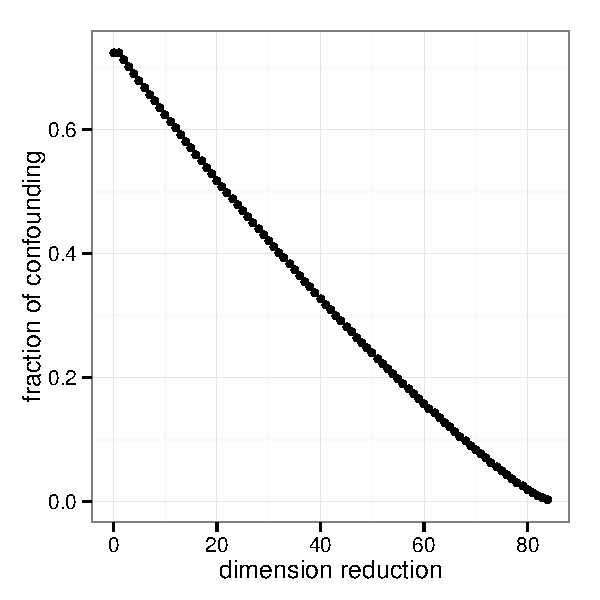
\includegraphics[width=0.4\textwidth]{radon_elbow1.pdf}
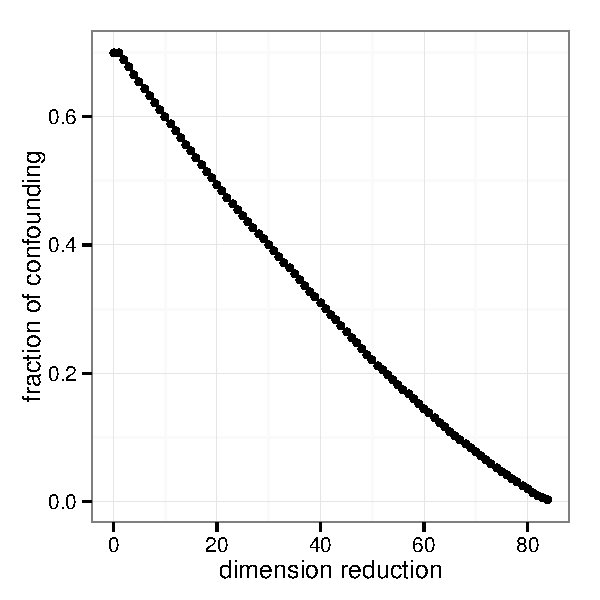
\includegraphics[width=0.4\textwidth]{radon_elbow2.pdf}

\begin{table}[ht]
\centering
\caption{\label{tab:s} The fraction of confounding for the rotated random effects at various settings of $s$ for model \eqref{eq:radon}. \hh{At which dimension does the normality test switch from rejection to acceptance?} \al{This happens right away, rank(B), for the slope and around 40 for the intercept.}}
\begin{tabular}{rrrrrrr}
  \hline
subspace dimension  $s$         & 30 & 40 & 50 & 60 & 70 & 80 \\ \hline
  Intercept & 0.56 & 0.60 & 0.63 & 0.66 & 0.69 & 0.72 \\ 
  Slope     & 0.52 & 0.56 & 0.60 & 0.63 & 0.66 & 0.70 \\ 
   \hline
\end{tabular}
\end{table}
%
Based on  Table~\eqref{tab:s} we choose $s=30$ for the calculation of the rotated random effects. Figure~\ref{fig:rotate-radon} shows Q-Q plots of the marginal rotated random effects, which do not exhibit \hh{significant} deviations from the assumption of normality.



\begin{figure}[htb]
	\centering
	 \subfloat[Random intercept]{
		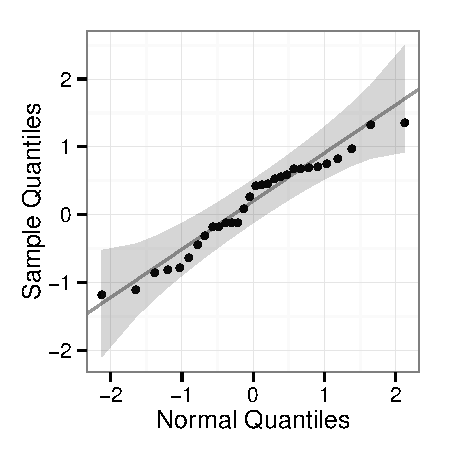
\includegraphics[width=0.35\linewidth]{rotatedQQ-intercept.pdf}
		}
	  \subfloat[Random slope]{
		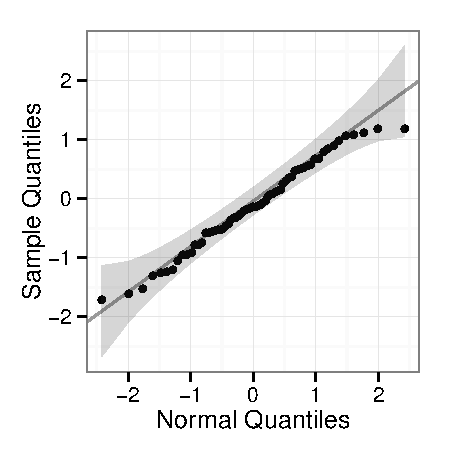
\includegraphics[width=0.35\linewidth]{rotatedQQ-slope.pdf}
		}	
	\caption{\label{fig:rotate-radon} Normal Q-Q plots with point-wise 95\% confidence bands of the marginals rotated random effects. The deviations from normality are much less pronounced than before resulting in the failure to reject the null hypothesis of normality.} %\hh{what do the normality tests say?} \al{The tests all say fail to reject.}}
\end{figure}

%\begin{itemize}
%\item Show Q-Q plots for the rotated random effects
%\item Discuss choice of $s$ in this example
%\item Recap root of the problems with the raw random effects (errors not normally distributed; large degree of pooling/shrinkage)
%\end{itemize}

%----------------------------------------------------------------------------------
\section{Discussion}\label{sec:discussion}
%----------------------------------------------------------------------------------

In this paper we have discussed two graphical approaches to assess the distributional assumptions made on the random effects in hierarchical linear models. The first approach used the lineup protocol to compare the predicted random effects produced in estimating observed model to those produced when estimating a properly specified model. This method only assumes a distributional specification for the random effects and does not directly compare the predicted random effects to their hypothesized distribution. Consequently, the conclusions that are drawn from this approach relate to evidence that the predicted random effects either are or are not \hh{consistent} with what is expected under a correctly specified random effects distribution. The second approach rotates the predicted random effects so as to compare them directly to the hypothesized distribution using a Q-Q plot. We have shown that the rotated random effects are standardized, uncorrelated, and homoscedastic, and that the rotation addressing the confounding present allowing for the random effects to be targeted separately from the error terms. While the loss in power due to the rotation may be troubling, we found the lack of diagnostic information in the predicted random effects to be the bigger concern. \al{XX The last sentence might not be needed if we keep the last paragraph as it is.}

Under either approach, a misspecified covariance structure may lead to erroneous rejection of the null hypothesis. Therefore, in practice we recommend an assessment of the structure of \al{the within- and between-group covariance matrices} prior to distributional assessment.
%\todo[inline]{R and D have been introduced way back - rather than using the symbols, describe the matrices in words.}. 
An alternative approach would be the use of robust covariance estimation techniques to protect against such misspecification; however, \hh{it is not clear how this impacts the diagnostic tools. We will leave this investigation for future study.} %we are unsure of its impact on these diagnostic tools, which is an are for future study.

It is important to note that formal tests have been proposed  to detect mixture distributions in the random effects \citep{Verbeke:1996va} and for overall goodness-of-fit tests for both the error terms and random effects \citep{Jiang:2001up}; however, these methods do \hh{not} lend themselves to graphical inspection and have not been implemented in statistical software. Our method, on the other hand, requires only byproducts of the model fitting procedure and the use of matrix decompositions for simultaneous diagonalization, which are \hh{ widely accessible in standard software.}
%Following from this result, the pointwise confidence bands shown were not unique to this method, but follow from the development of the normal Q-Q plot (FIND REFERENCE), and were provided as an aid to interpretation, not as a formal test.

%\todo[inline]{The paragraphs below here need to be reworked/rethought based on the rewritten paragraphs above.}

Simulation has revealed that tests of normality using the rotated random effects achieve approximately nominal type I error rates with appropriate choice of the \al{dimension}, $s$. This indicates that assessment of the rotated residuals can target the distribution of the random effects in the presence of pooling, which the predicted random effects cannot. The power to detect non-normal random effects distributions is lower than the gold standard, which is to be expected as \hh{the rotated residuals consist of sums of predicted random effects, resulting in a total distribution that is closer to a normal distribution than its individuals. } %we have taken linear combinations of predicted random effects in our rotation. 
The varimax rotation \hh{ reduces} the impact of this supernormality effect. %, but other orthogonal rotations (i.e., quartimax) may perform better resulting in increased power and is an area for future investigation. 
\hh{While we do think that the loss in power is troubling, }
%We believe the loss of power is less troubling than
 the inflated type I error rates resulting from high levels of confounding \hh{is of a much bigger concern.}
 \hh{Unlike before,  any} detection of a distributional deviation \hh{can now be trusted even in situations with high amounts of  confounding between the levels of residuals}.
  
%  This indicates that the predicted random effects do contain useful diagnostic information even when models are highly confounded, but not in their ``raw'' state.
 
%It is important to note that the procedure outlined in this paper assumes that the covariance structures in the hierarchical linear model are correctly specified. If this is not the case, then we would expect this model violation to affect assessment of the rotated random effect. Therefore, in practice we recommend an assessment of the covariance structures prior to distributional assessment. It would be of interest to assess the effectiveness of this methodology with robust covariance estimation techniques.

%\todo[inline]{Should I talk about the more alternative objective function that I have recently discovered that might lead to better results but is computationally more complex as there is no closed form solution? I see this as an area of future investigation, but I don't know how much of that is conventional to put in the article.}

%\todo[inline]{Things to return to in the discussion (moved from elsewhere)}
%\hh{the next paragraph needs a bit of attention. my first reaction as a reviewer would be to say - ok, it's not graphical, but how do those tests do? It distracts a bit from the main intention of the paper. I'd be in favor to remove the paragraph from here and maybe leave it for the discussion that there are other , non-graphical tests. }
%\al{I see your point. I will work on incorporating this to the discussion.}
%Several methods to assess the random effects distribution have been proposed. Formal tests have been proposed to to detect mixture distributions \citep{Verbeke:1996va} in the random effects and for overall goodness-of-fit tests for both the error terms and random effects \citep{Jiang:2001up}; however, these methods do \hh{not} lend themselves to graphical inspection and have not been implemented in statistical software.


% If a graphical assessment of the random effects distribution is not desired, then there are other available methods for model assessment \cite[c.f., the $\chi^2$ test proposed by][]{Jiang:2001up}, but they do not lend themselves to graphical inspection. While such goodness-of-fit tests can detect distributional deviations, they do not suggest how the assumption as been violated. 

%The rotated random effects can be used with Q-Q plots, which are familiar to analysts. 
%The use of the rotated random effects results in approximately nominal type I error rates when the dimension, $s$, is properly chosen; however, simulations have revealed that tests using the rotated random effects have low power to detect non-normal alternatives. Despite this fact, the rotated random effects present a method allowing for the predicted random effects to be used in distributional assessment, and when a deviation is detected one has cause to believe this detection, which previously not the case for highly confounded models. Additionally, this method is far less computationally demanding than simulation-based assessments, such as simulation envelopes for Q-Q plots, which are not guaranteed to work in situations with high levels of confounding (see the supplemental materials). Also, orthogonal rotations other than the varimax rotation (such as the quartimax rotation) may provide additional power, and is an area for future investigation. 



%\todo[inline]{
%Summarize everything and talk about future directions (if there are any). I have started a list below}
%\begin{itemize}
%\item Discuss the relative speed of this procedure to a bootstrap procedure
%\item Discuss why we are not using the ``upward'' residuals analysis approach discussed in the lit review chapter.
%\end{itemize}



%----------------------------------------------------------------------------------
\section*{Appendix: Additional technical details}
%----------------------------------------------------------------------------------

We present the proof of the claim that the rotated residuals, $\bm{W}^{*\prime} \widehat{\bm{b}}$, are standardized, uncorrelated, and homoscedastic. Following the developments presented in Section~\ref{sec:rotate}, we present this discussion for the random effects assuming that there is only a random intercept. Generalization to the situation with multiple random effects follows as previously discussed.

\begin{proof}
 Let $\bm{A} = \var(\widehat{\bm{b}} | \bm{b})$, $\bm{B} = \var(\widehat{\bm{b}})$, $r = \text{rank}(\bm{B})$, and $q = $ the number of elements in $\widehat{\bm{b}}$. Note that by definition $\bm{A}$ and $\bm{B}$ are symmetric and positive semidefinite. Following from above, $\bm{T}_r$ and $\bm{\Lambda}_r$ follow from the spectral (or eigenvalue) decomposition of $\bm{B} = \bm{T_r \Lambda_r T_r}\trans$, and $\bm{U}$ follows from the spectral decomposition of $\bm{A^*} = \bm{\Lambda_r}^{-1/2} \bm{T_r}\trans \bm{A T_r \Lambda_r}^{-1/2} = \bm{U} \bm{\Gamma} \bm{U}\trans$. Then, 
\begin{align*}
\var(\bm{W}^{*\prime} \widehat{\bm{b}}) &= \var(\bm{U}\trans \bm{\Lambda_r}^{-1/2} \bm{T_r}\trans \widehat{\bm{b}})\\
&= (\bm{U}\trans \bm{\Lambda_r}^{-1/2} \bm{T_r}\trans) \var(\widehat{\bm{b}}) (\bm{T_r \Lambda_r}^{-1/2} \bm{U})\\
&= (\bm{U}\trans \bm{\Lambda_r}^{-1/2} \bm{T_r}\trans) \bm{B} (\bm{T_r \Lambda_r}^{-1/2} \bm{U})\\
&= \bm{I}
\end{align*}
proving that the rotated errors are standardized, uncorrelated, and homoscedastic.
\end{proof}
 
%Recall that the trace of a matrix is equal to the sum of its eigenvalues; therefore, minimizing $\tr\left( \bm{B}\ginv\bm{A} \right)$ is equivalent to minimizing the sum of the eigenvalues of $\bm{B}\ginv\bm{A}$. The eigenvalues of $\bm{B}\ginv\bm{A}$ can be found through simultaneous diagonalization
% 
% 
%Write the spectral decomposition of $\bm{B}$ as
%$\bm{B} = \bm{T_r \Lambda_r T_r}\trans$, where $\bm{ \Lambda_r}$ is a diagonal matrix of the nonzero eigenvalues and $\bm{T_r}$ is the matrix of associated eigenvectors.
%Define $\bm{F} = \bm{T_r \Lambda_r}^{1/2}$, which is a full-rank decomposition of $\bm{B}$. The Moore-Penrose inverse of $\bm{F}$ is given by
%\[
%\bm{F}\ginv = (\bm{F}\trans\bm{F})\inv \bm{F}\trans = \bm{\Lambda_r}^{-1/2} \bm{T_r}\trans
%\]
%Now, notice that
%\[
%\bm{F}\ginv \bm{B} (\bm{F}\ginv)\trans = \bm{\Lambda_r}^{-1/2} \bm{T_r}\trans ( \bm{T_r \Lambda_r T_r}\trans ) \bm{T_r \Lambda_r}^{-1/2} =  \bm{I}
%\]
%and define
%\[
%	\bm{A}^* = \bm{F}\ginv \bm{A} (\bm{F}\ginv)\trans
%\]
%Next, we rewrite $\bm{W} = (\bm{F}\ginv)\trans \bm{U}$, where $\bm{U}$ is a nonsingular symmetric matrix. Then \eqref{eq:app1} becomes
%%
%\begin{equation}\label{eq:app2}
%\tr \left[ \left( \bm{U}\trans \bm{F}\ginv \bm{B} (\bm{F}\ginv)\trans \bm{U} \right)\inv 
%\left(\bm{U}\trans \bm{F}\ginv \bm{A} (\bm{F}\ginv)\trans \bm{U} \right) \right]
%=
%\tr \left[ \left( \bm{U}\trans \bm{I} \bm{U} \right)\inv \left( \bm{U}\trans \bm{A}^* \bm{U} \right) \right]
%\end{equation}
%%
%whose derivative with respect to $\bm{U}$ is given by
%%
%\begin{equation}\label{eq:app3}
%-2 \bm{IU} \left( \bm{U}\trans \bm{I} \bm{U} \right)\inv \left( \bm{U}\trans \bm{A}^* \bm{U} \right) \left( \bm{U}\trans \bm{I} \bm{U} \right)\inv + 2 \bm{A}^* \bm{U} \left( \bm{U}\trans \bm{I} \bm{U} \right)\inv
%\end{equation}
%%
%\citep[A.16]{Fukunaga:1990}. Setting \eqref{eq:app3} to zero we find that the solution must satisfy
%%
%\begin{equation}
%\bm{A}^* \bm{U} = \bm{U} \left( \bm{U}\trans \bm{A}^* \bm{U} \right)
%\end{equation}
%%
%
%
%which is of the form of an eigenvalue problem, which is minimized at the eigenvector corresponding to the smallest eigenvalue of  $\bm{A}^*$. Additionally, the value of \eqref{eq:app2} lies between the minimum and maximum eigenvalue of $\bm{A}^*$.
%
%The requirement that $\bm{W}$ be of full rank results in $\bm{W} = \bm{T_r \Lambda_r}^{-1/2} \bm{U}$, where $\bm{U}$ are the eigenvectors of $\bm{A}^*$.
%\end{proof}
%
%More general proofs can be found in \cite{McDonald:1979ca} and \cite{deLeeuw:1982to}.
%
%Next we show that the resulting residuals are standardized, uncorrelated, and homoscedastic.
%
%\begin{proof} Carrying through the notation from above we see that
%\begin{align*}
%\var(\bm{W}^{*\prime} \widehat{\bm{e}}) &= \var(\bm{U}\trans \bm{\Lambda_r}^{-1/2} \bm{T_r}\trans \widehat{\bm{e}})\\
%&= (\bm{U}\trans \bm{\Lambda_r}^{-1/2} \bm{T_r}\trans) \var(\widehat{\bm{e}}) (\bm{T_r \Lambda_r}^{-1/2} \bm{U})\\
%&= (\bm{U}\trans \bm{\Lambda_r}^{-1/2} \bm{T_r}\trans) \bm{B} (\bm{T_r \Lambda_r}^{-1/2} \bm{U})\\
%&= \bm{I}
%\end{align*}
%
%\end{proof}


%----------------------------------------------------------------------------------
%----------------------------------------------------------------------------------
\todo[inline]{Currently the references also include those for the supplements, so there may be a few extra because of this.}
\bibliographystyle{apa}
\bibliography{lcresid_bib}
%----------------------------------------------------------------------------------
%----------------------------------------------------------------------------------

\clearpage

%----------------------------------------------------------------------------------
\appendix
\section{Supplement to ``Are you Normal? The Problem of Confounded Residual Structures in Hierarchical Linear Models''}
%----------------------------------------------------------------------------------

The materials in this document supplement the information presented in ``Are you Normal? The Problem of Confounded Residual Structures in Hierarchical Linear Models''. Section~\ref{supp:evals} presents a simulation study evaluating the performance of existing proposals for residual analysis for hierarchical linear models. Section~\ref{supp:simstudy} presents the complete results for all simulation settings considered in the paper. 


\subsection{Evaluations of existing proposals}\label{supp:evals}
%--------------------------------------------------

\subsubsection{Model notation}
%--------------------------
Recall that the stacked representation of the hierarchical linear model is given by 
%
\begin{align}\label{eq:hlm}
	\underset{(n \times 1)}{\bm{y}} &= \underset{(n_i \times p)}{\bm{X}} \ \underset{(p \times 1)}{\bm{\beta}} + \underset{(n \times q)}{\bm{Z}_i} \ \underset{(q \times 1)}{\bm{b}} + \underset{(n \times 1)}{\bm{\varepsilon}},\\
	\bm{\varepsilon} & \overset{\text{iid}}{\sim} \mathcal{N}(\bm{0}, \ \bm{R}), \qquad \bm{b} \overset{\text{iid}}{\sim} \mathcal{N}(\bm{0},\ \bm{D}) \nonumber
\end{align}
%
where $\bm{y}$ is a vector of responses, $\bm{X}$ and $\bm{Z}_i$ are design matrices for the fixed and random effects, respectively, $\bm{\beta}$ is a vector of fixed effects, $\bm{b}$ is a vector of random effects, $\bm{\varepsilon}_i$ is a vector of error terms, and $\bm{R}$ and $\bm{D}$ are positive definite covariance matrices. Further, we assume that $\cov(\bm{\varepsilon},\ \bm{b}) = \bm{0}$. The above assumptions imply that, marginally, $\bm{y} \sim \mathcal{N}(\bm{X\beta},\ \bm{V})$ where $\bm{V} = \bm{ZDZ}\trans$.

\subsubsection{Residuals}

In this section we consider residuals that are commonly used to check the distributional assumptions in a hierarchical linear model. For more general discussions of residual analysis for hierarchical linear models we refer the reader to \cite{Haslett:2007vv} and \cite{Nobre:2007ej}.

\paragraph{Marginal residuals.} 
%-----------------------------
The marginal distribution of $\bm{y}$ leads to the marginal residuals which are defined as
%
\begin{equation}\label{eq:marginalresid}
\widehat{\bm{\zeta}}  = \bm{y} - \bm{X} \widehat{\bm{\beta}} =  \bm{V P y}
\end{equation}
%
where $ \bm{P} = \bm{V\inv} - \bm{V\inv X} \left( \bm{X\trans V\inv X} \right) \bm{X \trans V\inv}$, which reveal how the observations deviate from the global trend. The use of these residuals for distributional assessment provides an omnibus assessment of goodness-of-fit as the marginal residuals are a linear combination of the other residual quantities; however, this assessment requires the empirical distribution of the marginal residuals to resemble true distribution. Asymptotically, the variance of the marginal residuals is $\var(\widehat{\zeta}) = \bm{V}$ leading to correlated residuals. To obtain asymptotically uncorrelated residuals the marginal residuals can be scaled by the Cholesky root of $\bm{V}$ \citep{Houseman:2004gq}, $\bm{C}$, yielding
%
\begin{equation}\label{eq:choleskyresid}
\bm{z}_{\zeta}  = \bm{C}\inv \widehat{\bm{\zeta}}
\end{equation}
%


\paragraph{Level-1 residuals.}
%-----------------------------
The distribution of $\bm{y}$ conditional on the random effects, $\bm{b}$, is given by
%
\begin{equation}\label{eq:marginalmodel}
	\bm{y} | \bm{b} \sim \mathcal{N}( \bm{X\beta} + \bm{Zb},\ \bm{R} ),
\end{equation}
%
and leads to the level-1 residuals, commonly referred to as the error terms, which are defined as
%
\begin{equation}\label{eq:lev1resid}
	\widehat{\bm{\varepsilon}} = \bm{y} - \bm{X \widehat{\beta}} + \bm{Z \widehat{b}} = \bm{R P y}
\end{equation}
%
and reveal the deviations of the observations from the conditional model. The variance of the level-1 residuals is given by $\var(\widehat{\bm{\varepsilon}}) = \bm{ R P R }$, so studentized level-1 residuals can be obtained by 
%
\begin{equation}\label{eq:lev1-std}
\bm{z}_{\varepsilon} =  \text{diag} \left(\bm{RPR} \right)^{-1/2} \widehat{\bm{\varepsilon}}
\end{equation}
%
which have been recommended for distributional assessment \citep{Nobre:2007ej}. An alternative approach is recommended by \citet[Section 4.3]{Pinhiero:2000vf}, who suggest use of the Pearson residuals, which are obtained by dividing the predicted residuals by the estimated within-group standard deviation, $\widehat{\sigma}_\varepsilon$. 



\paragraph{Level-2 residuals.}
%-----------------------------
The final type of residual we consider is the the best linear unbiased predictor (BLUP) of the random effects (i.e., predicted random effects), providing insight into the differences between the marginal (global) and conditional models. By definition, the BLUP of $\bm{b}$ is
%
\begin{equation}\label{eq:lev2resid}
\widehat{\bm{b}} = \bm{D Z\trans V\inv} \left( \bm{y} - \bm{X \widehat{\beta}} \right) = \bm{D Z\trans P y}
\end{equation}
%
which has variance $\var(\widehat{\bm{b}}) = \bm{DZ\trans P ZD}$. 
%Rewriting $\var(\widehat{\bm{b}})$ as
%%
%\begin{equation}
%\bm{DZ\trans P ZD} = \bm{DZ\trans} \bm{V\inv} \left( \bm{V} - \bm{ X} \left( \bm{X\trans V\inv X} \right) \bm{X \trans} \right) \bm{V\inv} \bm{ZD}
%\end{equation}
%%
%leads to two 
For distributional assessment of the BLUPs it makes sense to examine each random effect individually, though \cite{Lange:1989uu} suggest the examination of linear combinations of standardized BLUPs. Rewritting the definition of $\var(\widehat{\bm{b}})$
%
\begin{equation}
\bm{DZ\trans P ZD} = \bm{DZ\trans} \bm{V\inv} \left( \bm{V} - \bm{ X} \left( \bm{X\trans V\inv X} \right) \bm{X \trans} \right) \bm{V\inv} \bm{ZD}
\end{equation}
%
leads to two similar standardizations of the BLUPs. The first utilizes the fact that when the number of groups is large $\bm{ X} \left( \bm{X\trans V\inv X} \right)$ will be small \citep{Goldstein:2003}, so for a large number of groups standardized BLUPs can be calculated by
%
\begin{equation}\label{eq:lev2-std1}
\bm{z}_{b} = \text{diag} \left(\bm{DZ\trans V\inv ZD}\right)^{-1/2} \widehat{\bm{b}}
\end{equation}
%
This formulation is the same used by \cite{Lange:1989uu} (discussed below).
%, who suggest creating weighted Q-Q plots \citep{Dempster:1985tr} to assess the distributional assumptions. Note that standardized linear combinations of the BLUPs follow in the usual way. 
The second standardization applies for all sample sizes and is given by
%
\begin{equation}\label{eq:lev2-std2}
\bm{z}_{b} = \text{diag} \left(\bm{DZ\trans P ZD}\right)^{-1/2} \widehat{\bm{b}}
\end{equation}
%


\paragraph{Weighted Q-Q plots}
%------------------------------

As an alternative to Q-Q plots constructed from the BLUPs \cite{Lange:1989uu} propose using weighted Q-Q plots of standardized linear combinations of the BLUPs, $\bm{C\trans}\widehat{\bm{b}}$,
%
\begin{equation}
z_{b} = \text{diag} \left(\bm{C\trans DZ\trans V\inv ZDC}\right)^{-1/2} \bm{C\trans}\widehat{\bm{b}}
\end{equation}
%
The specific form of $\bm{C}$ chosen highlights different departures from distributional assumptions---for example, $\bm{C}$s can be chosen to extract the random slope and the random intercept terms individually. When the random effects may be correlated, \citeauthor{Lange:1989uu} suggest examining a range of additional linear combinations in-between the two marginal random effects either through manual specification of $\bm{C}$ or projection pursuit.
After choosing $\bm{C}$ a weighted Q-Q plot is constructed by comparing the weighted empirical cumulative distribution function
%
\begin{equation}
F_m^*(x) = \sum_{i=1}^{m} I(x - z_{b_i} \geq 0) w_i \bigg/ \sum_{i=1}^{m} w_i, 
\end{equation}
%
to $\Phi\inv \left ( F_m^*(z_{b_i}) \right)$. Here, $w_i$ is the $i$th element of $\bm{C\trans DZ\trans V\inv ZDC}$.
For balanced group sizes this simplifies to the unweighted Q-Q plot of $\bm{z}_b$.
%

\paragraph{Simulation-based approaches}
%---------------------------------------

All of the above approaches to checking the distributional assumptions rely on the use of interrelated residuals, which has been reported to be problematic \citep{HildenMinton:1995wh, Verbeke:1996va}.  
One alternative that has been proposed to overcome this problem is the use of the parametric bootstrap to develop point-wise and simultaneous confidence bands for Q-Q plots. We evaluate the potential of this method using bootstrap tests of normality.


\subsubsection{Simulation study}\label{supp:simstudy}
%--------------------------------------------------

To evaluate the above proposals we carried out a simulation study under the same settings as in the paper, with the only difference being that the original $\bm{Z}$ was used for data generation. To evaluate the bootstrap tests of normality, a null distribution of 5000 simulated test statistics for each situation was used.

Tables~\ref{tab:eval1}--\ref{tab:evalmarginal} present the results of using standard normality tests to assess the distributional assumptions of the residuals from a hierarchical model. The gray background on the table indicates which simulation settings present estimated type I error, with the other rows presenting estimated power. Tables~\ref{tab:boot1}--\ref{tab:bootmarginal} present the results of the bootstrap tests for normality. Table~\ref{tab:langeryan} presents the results of using a weighted CDF to evaluate the normality of the random effects, in this case the null distribution was obtained using the parametric bootstrap.

Based on the simulation results it is clear that none of the residual-based diagnostics for assessing distributional assumptions are appropriate in all situations. The error terms can be targeted either by the use of studentized residuals or a parametric bootstrap; however, the assessment of this assumption is less critical. The random effects, on which predictive inference relies, cannot be targeted by the current methods when the residual variance is larger than the variance component associated with the random effects---that is, situations with higher degrees of shrinkage.  Such situations are often encountered in practice. Additionally, use of the parametric bootstrap---to construct simulation envelopes for Q-Q plots, for example---does not appear to remedy this situation based on the performance of the bootstrap tests. Finally, we have shown \citeauthor{Lange:1989uu}'s weighted Q-Q plots cannot target the random effects distribution when the residual variance is large, as the distribution of the error terms overly influences tests for the random slope, resulting in inflated type I error rates for both random effects.

%&&&&&&&&&&&&&&&&&&&&&&&&&&&&&&&&&&&&&&&&&&&&&&&&&&&&&&&&&&&&&&&&&&&&&&&&&&&&&&
% Correct model
%&&&&&&&&&&&&&&&&&&&&&&&&&&&&&&&&&&&&&&&&&&&&&&&&&&&&&&&&&&&&&&&&&&&&&&&&&&&&&&


%------------------------------------------------
% Naive tests
%------------------------------------------------

%%% Level-1 residuals
\begin{table}[ht]
\centering
\caption{\label{tab:eval1} Proportion of tests rejecting the null hypothesis of normality of the error terms.}
\begin{scriptsize}
\begin{tabular}{ll p{.1cm} c p{.1cm} rrr p{.1cm} rrr p{.1cm} rrr}
  \hline
  \multicolumn{2}{c}{Distributions}& & Nominal & &  \multicolumn{3}{c}{Raw residuals} & & \multicolumn{3}{c}{Pearson residuals} & & \multicolumn{3}{c}{Studentized residuals}\\ \cline{1-2} \cline{6-8} \cline{10-12} \cline{14-16}
  Errors & Random effects & & $\alpha$ & & AD & CVM & KS & & AD & CVM & KS & & AD & CVM & KS \\ 
   \hline
& && && \multicolumn{9}{c}{$\sigma_{\varepsilon}^2 = 4$, \ \ $\sigma_{b_0}^2 = \sigma_{b_1}^2 = 1$} \\ \cline{6-16}

\rowcolor{gray!20} Normal       & Normal       && 0.05 && 0.07 & 0.06 & 0.06 && 0.07 & 0.06 & 0.06 && 0.04 & 0.04 & 0.04 \\ 
\rowcolor{gray!20}             &              && 0.10 && 0.13 & 0.12 & 0.12 && 0.13 & 0.12 & 0.12 && 0.09 & 0.09 & 0.10 \\ 
\rowcolor{gray!20}             & Heavy tailed && 0.05 && 0.07 & 0.08 & 0.06 && 0.07 & 0.08 & 0.06 && 0.05 & 0.05 & 0.05 \\ 
\rowcolor{gray!20}             &              && 0.10 && 0.14 & 0.13 & 0.14 && 0.14 & 0.13 & 0.14 && 0.11 & 0.11 & 0.10 \\ 
\rowcolor{gray!20}             & Skewed       && 0.05 && 0.07 & 0.06 & 0.06 && 0.07 & 0.06 & 0.06 && 0.04 & 0.04 & 0.05 \\ 
\rowcolor{gray!20}             &              && 0.10 && 0.13 & 0.12 & 0.13 && 0.13 & 0.12 & 0.13 && 0.09 & 0.09 & 0.10 \\ 
             &&&&&&&&&&&&&&&\\
Heavy tailed & Normal       && 0.05 && 1.00 & 1.00 & 1.00 && 1.00 & 1.00 & 1.00 && 1.00 & 1.00 & 1.00 \\ 
             &              && 0.10 && 1.00 & 1.00 & 1.00 && 1.00 & 1.00 & 1.00 && 1.00 & 1.00 & 1.00 \\ 
             & Heavy tailed && 0.05 && 1.00 & 1.00 & 1.00 && 1.00 & 1.00 & 1.00 && 1.00 & 1.00 & 1.00 \\ 
             &              && 0.10 && 1.00 & 1.00 & 1.00 && 1.00 & 1.00 & 1.00 && 1.00 & 1.00 & 1.00 \\ 
             & Skewed       && 0.05 && 1.00 & 1.00 & 1.00 && 1.00 & 1.00 & 1.00 && 1.00 & 1.00 & 1.00 \\ 
             &              && 0.10 && 1.00 & 1.00 & 1.00 && 1.00 & 1.00 & 1.00 && 1.00 & 1.00 & 1.00 \\ 
             &&&&&&&&&&&&&&&\\
Skewed       & Normal       && 0.05 && 1.00 & 1.00 & 1.00 && 1.00 & 1.00 & 1.00 && 1.00 & 1.00 & 1.00 \\ 
             &              && 0.10 && 1.00 & 1.00 & 1.00 && 1.00 & 1.00 & 1.00 && 1.00 & 1.00 & 1.00 \\ 
             & Heavy tailed && 0.05 && 1.00 & 1.00 & 1.00 && 1.00 & 1.00 & 1.00 && 1.00 & 1.00 & 1.00 \\ 
             &              && 0.10 && 1.00 & 1.00 & 1.00 && 1.00 & 1.00 & 1.00 && 1.00 & 1.00 & 1.00 \\ 
             & Skewed       && 0.05 && 1.00 & 1.00 & 1.00 && 1.00 & 1.00 & 1.00 && 1.00 & 1.00 & 1.00 \\ 
             &              && 0.10 && 1.00 & 1.00 & 1.00 && 1.00 & 1.00 & 1.00 && 1.00 & 1.00 & 1.00 \\ 

&&&&&&&&&&&&&&&\\
& && && \multicolumn{9}{c}{$\sigma_{\varepsilon}^2 = 1$, \ \ $\sigma_{b_0}^2 = \sigma_{b_1}^2 = 1$} \\ \cline{6-16}

\rowcolor{gray!20} Normal       & Normal       && 0.05 &&  0.05 & 0.05 & 0.04 && 0.05 & 0.05 & 0.04 && 0.04 & 0.04 & 0.04 \\ 
\rowcolor{gray!20}              &              && 0.10 &&  0.11 & 0.10 & 0.09 && 0.11 & 0.10 & 0.09 && 0.09 & 0.09 & 0.08 \\ 
\rowcolor{gray!20}              & Heavy tailed && 0.05 &&  0.07 & 0.06 & 0.06 && 0.07 & 0.06 & 0.06 && 0.05 & 0.06 & 0.05 \\ 
\rowcolor{gray!20}              &              && 0.10 &&  0.13 & 0.12 & 0.11 && 0.13 & 0.12 & 0.11 && 0.11 & 0.11 & 0.10 \\ 
\rowcolor{gray!20}              & Skewed       && 0.05 &&  0.05 & 0.05 & 0.05 && 0.05 & 0.05 & 0.05 && 0.04 & 0.04 & 0.04 \\ 
\rowcolor{gray!20}              &              && 0.10 &&  0.10 & 0.09 & 0.11 && 0.10 & 0.09 & 0.11 && 0.08 & 0.09 & 0.10 \\ 
              &&&&&&&&&&&&&&&\\
 Heavy tailed & Normal       && 0.05 &&  1.00 & 1.00 & 1.00 && 1.00 & 1.00 & 1.00 && 1.00 & 1.00 & 1.00 \\ 
              &              && 0.10 &&  1.00 & 1.00 & 1.00 && 1.00 & 1.00 & 1.00 && 1.00 & 1.00 & 1.00 \\ 
              & Heavy tailed && 0.05 &&  1.00 & 1.00 & 1.00 && 1.00 & 1.00 & 1.00 && 1.00 & 1.00 & 1.00 \\ 
              &              && 0.10 &&  1.00 & 1.00 & 1.00 && 1.00 & 1.00 & 1.00 && 1.00 & 1.00 & 1.00 \\ 
              & Skewed       && 0.05 &&  1.00 & 1.00 & 1.00 && 1.00 & 1.00 & 1.00 && 1.00 & 1.00 & 1.00 \\ 
              &              && 0.10 &&  1.00 & 1.00 & 1.00 && 1.00 & 1.00 & 1.00 && 1.00 & 1.00 & 1.00 \\ 
              &&&&&&&&&&&&&&&\\
 Skewed       & Normal       && 0.05 &&  1.00 & 1.00 & 1.00 && 1.00 & 1.00 & 1.00 && 1.00 & 1.00 & 1.00 \\ 
              &              && 0.10 &&  1.00 & 1.00 & 1.00 && 1.00 & 1.00 & 1.00 && 1.00 & 1.00 & 1.00 \\ 
              & Heavy tailed && 0.05 &&  1.00 & 1.00 & 1.00 && 1.00 & 1.00 & 1.00 && 1.00 & 1.00 & 1.00 \\ 
              &              && 0.10 &&  1.00 & 1.00 & 1.00 && 1.00 & 1.00 & 1.00 && 1.00 & 1.00 & 1.00 \\ 
              & Skewed       && 0.05 &&  1.00 & 1.00 & 1.00 && 1.00 & 1.00 & 1.00 && 1.00 & 1.00 & 1.00 \\ 
              &              && 0.10 &&  1.00 & 1.00 & 1.00 && 1.00 & 1.00 & 1.00 && 1.00 & 1.00 & 1.00 \\ 

&&&&&&&&&&&&&&&\\
& && && \multicolumn{9}{c}{$\sigma_{\varepsilon}^2 = 1$, \ \ $\sigma_{b_0}^2 = \sigma_{b_1}^2 = 4$} \\ \cline{6-16}

\rowcolor{gray!20} Normal       & Normal       && 0.05 &&  0.10 & 0.09 & 0.07 && 0.10 & 0.09 & 0.07 && 0.05 & 0.04 & 0.04 \\ 
\rowcolor{gray!20}             &              && 0.10 &&  0.17 & 0.17 & 0.15 && 0.17 & 0.17 & 0.15 && 0.09 & 0.09 & 0.09 \\ 
\rowcolor{gray!20}             & Heavy tailed && 0.05 &&  0.11 & 0.11 & 0.10 && 0.11 & 0.11 & 0.10 && 0.06 & 0.06 & 0.05 \\ 
\rowcolor{gray!20}             &              && 0.10 &&  0.19 & 0.19 & 0.19 && 0.19 & 0.19 & 0.19 && 0.12 & 0.11 & 0.12 \\ 
\rowcolor{gray!20}             & Skewed       && 0.05 &&  0.10 & 0.10 & 0.09 && 0.10 & 0.10 & 0.09 && 0.05 & 0.05 & 0.06 \\ 
\rowcolor{gray!20}             &              && 0.10 &&  0.18 & 0.18 & 0.17 && 0.18 & 0.18 & 0.17 && 0.11 & 0.11 & 0.11 \\ 
             &&&&&&&&&&&&&&&\\
Heavy tailed & Normal       && 0.05 &&  1.00 & 1.00 & 1.00 && 1.00 & 1.00 & 1.00 && 1.00 & 1.00 & 1.00 \\ 
             &              && 0.10 &&  1.00 & 1.00 & 1.00 && 1.00 & 1.00 & 1.00 && 1.00 & 1.00 & 1.00 \\ 
             & Heavy tailed && 0.05 &&  1.00 & 1.00 & 1.00 && 1.00 & 1.00 & 1.00 && 1.00 & 1.00 & 1.00 \\ 
             &              && 0.10 &&  1.00 & 1.00 & 1.00 && 1.00 & 1.00 & 1.00 && 1.00 & 1.00 & 1.00 \\ 
             & Skewed       && 0.05 &&  1.00 & 1.00 & 1.00 && 1.00 & 1.00 & 1.00 && 1.00 & 1.00 & 1.00 \\ 
             &              && 0.10 &&  1.00 & 1.00 & 1.00 && 1.00 & 1.00 & 1.00 && 1.00 & 1.00 & 1.00 \\ 
             &&&&&&&&&&&&&&&\\
Skewed       & Normal       && 0.05 &&  1.00 & 1.00 & 1.00 && 1.00 & 1.00 & 1.00 && 1.00 & 1.00 & 1.00 \\ 
             &              && 0.10 &&  1.00 & 1.00 & 1.00 && 1.00 & 1.00 & 1.00 && 1.00 & 1.00 & 1.00 \\ 
             & Heavy tailed && 0.05 &&  1.00 & 1.00 & 1.00 && 1.00 & 1.00 & 1.00 && 1.00 & 1.00 & 1.00 \\ 
             &              && 0.10 &&  1.00 & 1.00 & 1.00 && 1.00 & 1.00 & 1.00 && 1.00 & 1.00 & 1.00 \\ 
             & Skewed       && 0.05 &&  1.00 & 1.00 & 1.00 && 1.00 & 1.00 & 1.00 && 1.00 & 1.00 & 1.00 \\ 
             &              && 0.10 &&  1.00 & 1.00 & 1.00 && 1.00 & 1.00 & 1.00 && 1.00 & 1.00 & 1.00 \\ 


   \hline
\end{tabular}
\end{scriptsize}
\end{table}

%%% Level-2 residuals
\begin{table}[ht]
\centering
\caption{\label{tab:evalb0} Proportion of tests rejecting the null hypothesis of normality of the random intercept.}
\begin{scriptsize}
\begin{tabular}{ll p{.1cm} c p{.1cm} rrr p{.1cm} rrr p{.1cm} rrr}
  \hline
  \multicolumn{2}{c}{Distributions}& & Nominal & &  \multicolumn{3}{c}{Raw residuals} & & \multicolumn{3}{c}{Pearson residuals} & & \multicolumn{3}{c}{Studentized residuals}\\ \cline{1-2} \cline{6-8} \cline{10-12} \cline{14-16}
  Random effects & Errors & & $\alpha$ & & AD & CVM & KS & & AD & CVM & KS & & AD & CVM & KS \\ 
   \hline
& && && \multicolumn{9}{c}{$\sigma_{\varepsilon}^2 = 4$, \ \ $\sigma_{b_0}^2 = \sigma_{b_1}^2 = 1$} \\ \cline{6-16}

\rowcolor{gray!20} Normal       & Normal       && 0.05 &&   0.05 & 0.05 & 0.05 && 0.05 & 0.05 & 0.06 && 0.05 & 0.05 & 0.06 \\ 
\rowcolor{gray!20}             &              && 0.10 &&   0.10 & 0.10 & 0.10 && 0.11 & 0.10 & 0.12 && 0.11 & 0.10 & 0.12 \\ 
\rowcolor{gray!20}             & Heavy tailed && 0.05 &&   0.15 & 0.13 & 0.12 && 0.17 & 0.15 & 0.13 && 0.17 & 0.15 & 0.13 \\ 
\rowcolor{gray!20}             &              && 0.10 &&   0.22 & 0.20 & 0.20 && 0.26 & 0.23 & 0.21 && 0.26 & 0.23 & 0.20 \\ 
\rowcolor{gray!20}             & Skewed       && 0.05 &&   0.16 & 0.15 & 0.13 && 0.18 & 0.17 & 0.14 && 0.18 & 0.17 & 0.14 \\ 
\rowcolor{gray!20}             &              && 0.10 &&   0.25 & 0.23 & 0.21 && 0.28 & 0.25 & 0.22 && 0.28 & 0.25 & 0.21 \\ 
             &&&&&&&&&&&&&&&\\
Heavy tailed & Normal       && 0.05 &&   0.27 & 0.24 & 0.19 && 0.28 & 0.26 & 0.21 && 0.28 & 0.26 & 0.21 \\ 
             &              && 0.10 &&   0.35 & 0.31 & 0.28 && 0.36 & 0.34 & 0.30 && 0.36 & 0.33 & 0.30 \\ 
             & Heavy tailed && 0.05 &&   0.49 & 0.45 & 0.35 && 0.51 & 0.46 & 0.36 && 0.50 & 0.46 & 0.36 \\ 
             &              && 0.10 &&   0.58 & 0.54 & 0.46 && 0.60 & 0.55 & 0.47 && 0.60 & 0.55 & 0.47 \\ 
             & Skewed       && 0.05 &&   0.52 & 0.48 & 0.36 && 0.55 & 0.50 & 0.40 && 0.55 & 0.50 & 0.40 \\ 
             &              && 0.10 &&   0.62 & 0.59 & 0.51 && 0.65 & 0.60 & 0.53 && 0.65 & 0.60 & 0.52 \\
             &&&&&&&&&&&&&&&\\ 
Skewed       & Normal       && 0.05 &&   0.51 & 0.48 & 0.39 && 0.51 & 0.49 & 0.38 && 0.51 & 0.49 & 0.39 \\ 
             &              && 0.10 &&   0.61 & 0.58 & 0.51 && 0.61 & 0.59 & 0.52 && 0.60 & 0.58 & 0.52 \\ 
             & Heavy tailed && 0.05 &&   0.73 & 0.69 & 0.58 && 0.73 & 0.70 & 0.59 && 0.73 & 0.70 & 0.59 \\ 
             &              && 0.10 &&   0.80 & 0.77 & 0.69 && 0.81 & 0.78 & 0.70 && 0.80 & 0.78 & 0.70 \\ 
             & Skewed       && 0.05 &&   0.87 & 0.83 & 0.70 && 0.87 & 0.82 & 0.69 && 0.86 & 0.83 & 0.69 \\ 
             &              && 0.10 &&   0.92 & 0.89 & 0.80 && 0.91 & 0.88 & 0.80 && 0.91 & 0.88 & 0.80 \\ 

&&&&&&&&&&&&&&&\\
& && && \multicolumn{9}{c}{$\sigma_{\varepsilon}^2 = 1$, \ \ $\sigma_{b_0}^2 = \sigma_{b_1}^2 = 1$} \\ \cline{6-16}
\rowcolor{gray!20} Normal       & Normal       && 0.05 &&   0.05 & 0.05 & 0.04 && 0.05 & 0.05 & 0.04 && 0.05 & 0.05 & 0.04 \\ 
\rowcolor{gray!20}             &              && 0.10 &&   0.09 & 0.09 & 0.08 && 0.09 & 0.08 & 0.08 && 0.08 & 0.08 & 0.08 \\ 
\rowcolor{gray!20}             & Heavy tailed && 0.05 &&   0.07 & 0.07 & 0.06 && 0.07 & 0.07 & 0.06 && 0.07 & 0.07 & 0.06 \\ 
\rowcolor{gray!20}             &              && 0.10 &&   0.12 & 0.12 & 0.11 && 0.12 & 0.11 & 0.11 && 0.12 & 0.11 & 0.11 \\ 
\rowcolor{gray!20}             & Skewed       && 0.05 &&   0.06 & 0.06 & 0.07 && 0.06 & 0.06 & 0.06 && 0.06 & 0.06 & 0.06 \\ 
\rowcolor{gray!20}             &              && 0.10 &&   0.11 & 0.11 & 0.12 && 0.12 & 0.12 & 0.12 && 0.12 & 0.11 & 0.12 \\
             &&&&&&&&&&&&&&&\\  
Heavy tailed & Normal       && 0.05 &&   0.55 & 0.50 & 0.42 && 0.52 & 0.48 & 0.40 && 0.52 & 0.48 & 0.40 \\ 
             &              && 0.10 &&   0.63 & 0.60 & 0.51 && 0.60 & 0.56 & 0.51 && 0.60 & 0.56 & 0.52 \\ 
             & Heavy tailed && 0.05 &&   0.63 & 0.58 & 0.49 && 0.60 & 0.56 & 0.47 && 0.60 & 0.56 & 0.47 \\ 
             &              && 0.10 &&   0.71 & 0.68 & 0.60 && 0.68 & 0.63 & 0.56 && 0.68 & 0.63 & 0.56 \\ 
             & Skewed       && 0.05 &&   0.62 & 0.57 & 0.47 && 0.61 & 0.55 & 0.46 && 0.61 & 0.55 & 0.46 \\ 
             &              && 0.10 &&   0.71 & 0.66 & 0.58 && 0.69 & 0.65 & 0.57 && 0.69 & 0.64 & 0.57 \\ 
             &&&&&&&&&&&&&&&\\ 
Skewed       & Normal       && 0.05 &&   0.93 & 0.92 & 0.86 && 0.93 & 0.91 & 0.86 && 0.93 & 0.91 & 0.85 \\ 
             &              && 0.10 &&   0.96 & 0.94 & 0.91 && 0.96 & 0.94 & 0.90 && 0.95 & 0.94 & 0.90 \\ 
             & Heavy tailed && 0.05 &&   0.97 & 0.96 & 0.89 && 0.97 & 0.96 & 0.88 && 0.97 & 0.96 & 0.88 \\ 
             &              && 0.10 &&   0.99 & 0.98 & 0.94 && 0.99 & 0.98 & 0.94 && 0.99 & 0.98 & 0.94 \\ 
             & Skewed       && 0.05 &&   0.98 & 0.96 & 0.90 && 0.98 & 0.97 & 0.90 && 0.98 & 0.97 & 0.91 \\ 
             &              && 0.10 &&   0.99 & 0.97 & 0.95 && 0.99 & 0.98 & 0.94 && 0.99 & 0.98 & 0.95 \\ 


&&&&&&&&&&&&&&&\\
& && && \multicolumn{9}{c}{$\sigma_{\varepsilon}^2 = 1$, \ \ $\sigma_{b_0}^2 = \sigma_{b_1}^2 = 4$} \\ \cline{6-16}

\rowcolor{gray!20} Normal       & Normal       && 0.05 &&  0.05 & 0.05 & 0.05 && 0.05 & 0.05 & 0.04 && 0.05 & 0.05 & 0.04 \\ 
\rowcolor{gray!20}             &              && 0.10 &&  0.10 & 0.09 & 0.09 && 0.10 & 0.09 & 0.09 && 0.10 & 0.09 & 0.09 \\ 
\rowcolor{gray!20}             & Heavy tailed && 0.05 &&  0.04 & 0.04 & 0.05 && 0.05 & 0.05 & 0.05 && 0.05 & 0.05 & 0.05 \\ 
\rowcolor{gray!20}             &              && 0.10 &&  0.09 & 0.09 & 0.09 && 0.09 & 0.09 & 0.09 && 0.09 & 0.09 & 0.09 \\ 
\rowcolor{gray!20}             & Skewed       && 0.05 &&  0.04 & 0.04 & 0.03 && 0.04 & 0.04 & 0.03 && 0.04 & 0.04 & 0.03 \\ 
\rowcolor{gray!20}             &              && 0.10 &&  0.09 & 0.09 & 0.08 && 0.10 & 0.09 & 0.08 && 0.09 & 0.09 & 0.08 \\ 
             &&&&&&&&&&&&&&&\\
Heavy tailed & Normal       && 0.05 &&  0.68 & 0.63 & 0.54 && 0.68 & 0.63 & 0.54 && 0.68 & 0.63 & 0.54 \\ 
             &              && 0.10 &&  0.75 & 0.71 & 0.63 && 0.75 & 0.70 & 0.64 && 0.75 & 0.71 & 0.64 \\ 
             & Heavy tailed && 0.05 &&  0.71 & 0.67 & 0.57 && 0.71 & 0.67 & 0.58 && 0.71 & 0.67 & 0.57 \\ 
             &              && 0.10 &&  0.78 & 0.76 & 0.68 && 0.79 & 0.76 & 0.67 && 0.79 & 0.75 & 0.67 \\ 
             & Skewed       && 0.05 &&  0.70 & 0.68 & 0.57 && 0.70 & 0.67 & 0.56 && 0.70 & 0.67 & 0.56 \\ 
             &              && 0.10 &&  0.78 & 0.74 & 0.68 && 0.78 & 0.74 & 0.68 && 0.78 & 0.74 & 0.67 \\ 
             &&&&&&&&&&&&&&&\\
Skewed       & Normal       && 0.05 &&  1.00 & 0.99 & 0.97 && 1.00 & 0.99 & 0.97 && 1.00 & 0.99 & 0.97 \\ 
             &              && 0.10 &&  1.00 & 1.00 & 0.99 && 1.00 & 1.00 & 0.99 && 1.00 & 1.00 & 0.99 \\ 
             & Heavy tailed && 0.05 &&  1.00 & 1.00 & 0.98 && 1.00 & 1.00 & 0.98 && 1.00 & 1.00 & 0.98 \\ 
             &              && 0.10 &&  1.00 & 1.00 & 0.99 && 1.00 & 1.00 & 0.99 && 1.00 & 1.00 & 0.99 \\ 
             & Skewed       && 0.05 &&  1.00 & 1.00 & 0.98 && 1.00 & 1.00 & 0.98 && 1.00 & 1.00 & 0.98 \\ 
             &              && 0.10 &&  1.00 & 1.00 & 0.99 && 1.00 & 1.00 & 0.99 && 1.00 & 1.00 & 0.99 \\ 


   \hline
\end{tabular}
\end{scriptsize}
\end{table}


\begin{table}[ht]
\centering
\caption{\label{tab:evalb1} Proportion of tests rejecting the null hypothesis of normality of the random slope.}
\begin{scriptsize}
\begin{tabular}{ll p{.1cm} c p{.1cm} rrr p{.1cm} rrr p{.1cm} rrr}
  \hline
  \multicolumn{2}{c}{Distributions}& & Nominal & &  \multicolumn{3}{c}{Raw residuals} & & \multicolumn{3}{c}{Pearson residuals} & & \multicolumn{3}{c}{Studentized residuals}\\ \cline{1-2} \cline{6-8} \cline{10-12} \cline{14-16}
  Random effects & Errors & & $\alpha$ & & AD & CVM & KS & & AD & CVM & KS & & AD & CVM & KS \\ 
   \hline
& && && \multicolumn{9}{c}{$\sigma_{\varepsilon}^2 = 4$, \ \ $\sigma_{b_0}^2 = \sigma_{b_1}^2 = 1$} \\ \cline{6-16}

\rowcolor{gray!20} Normal       & Normal       && 0.05 &&   1.00 & 1.00 & 1.00 && 0.05 & 0.05 & 0.06 && 0.05 & 0.05 & 0.06 \\ 
\rowcolor{gray!20}             &              && 0.10 &&   1.00 & 1.00 & 1.00 && 0.10 & 0.10 & 0.10 && 0.10 & 0.10 & 0.10 \\ 
\rowcolor{gray!20}             & Heavy tailed && 0.05 &&   1.00 & 1.00 & 1.00 && 0.26 & 0.24 & 0.19 && 0.26 & 0.24 & 0.19 \\ 
\rowcolor{gray!20}             &              && 0.10 &&   1.00 & 1.00 & 1.00 && 0.35 & 0.32 & 0.27 && 0.35 & 0.32 & 0.27 \\ 
\rowcolor{gray!20}             & Skewed       && 0.05 &&   1.00 & 1.00 & 1.00 && 0.33 & 0.31 & 0.24 && 0.33 & 0.31 & 0.24 \\ 
\rowcolor{gray!20}             &              && 0.10 &&   1.00 & 1.00 & 1.00 && 0.41 & 0.38 & 0.34 && 0.41 & 0.38 & 0.34 \\ 
             &&&&&&&&&&&&&&&\\
Heavy tailed & Normal       && 0.05 &&   1.00 & 1.00 & 1.00 && 0.13 & 0.12 & 0.09 && 0.13 & 0.12 & 0.09 \\ 
             &              && 0.10 &&   1.00 & 1.00 & 1.00 && 0.18 & 0.19 & 0.17 && 0.18 & 0.19 & 0.17 \\ 
             & Heavy tailed && 0.05 &&   1.00 & 1.00 & 1.00 && 0.40 & 0.36 & 0.29 && 0.40 & 0.36 & 0.29 \\ 
             &              && 0.10 &&   1.00 & 1.00 & 1.00 && 0.49 & 0.44 & 0.37 && 0.49 & 0.45 & 0.37 \\ 
             & Skewed       && 0.05 &&   1.00 & 1.00 & 1.00 && 0.49 & 0.46 & 0.37 && 0.49 & 0.46 & 0.37 \\ 
             &              && 0.10 &&   1.00 & 1.00 & 1.00 && 0.59 & 0.56 & 0.50 && 0.59 & 0.56 & 0.49 \\
             &&&&&&&&&&&&&&&\\ 
Skewed       & Normal       && 0.05 &&   1.00 & 1.00 & 1.00 && 0.12 & 0.11 & 0.10 && 0.12 & 0.11 & 0.10 \\ 
             &              && 0.10 &&   1.00 & 1.00 & 1.00 && 0.17 & 0.16 & 0.16 && 0.18 & 0.16 & 0.16 \\ 
             & Heavy tailed && 0.05 &&   1.00 & 1.00 & 1.00 && 0.41 & 0.37 & 0.30 && 0.40 & 0.37 & 0.30 \\ 
             &              && 0.10 &&   1.00 & 1.00 & 1.00 && 0.51 & 0.47 & 0.39 && 0.51 & 0.47 & 0.39 \\ 
             & Skewed       && 0.05 &&   1.00 & 1.00 & 1.00 && 0.59 & 0.56 & 0.46 && 0.59 & 0.56 & 0.46 \\ 
             &              && 0.10 &&   1.00 & 1.00 & 1.00 && 0.70 & 0.66 & 0.58 && 0.70 & 0.66 & 0.58 \\ 

&&&&&&&&&&&&&&&\\
& && && \multicolumn{9}{c}{$\sigma_{\varepsilon}^2 = 1$, \ \ $\sigma_{b_0}^2 = \sigma_{b_1}^2 = 1$} \\ \cline{6-16}

\rowcolor{gray!20} Normal       & Normal       && 0.05 &&  1.00 & 1.00 & 1.00 && 0.05 & 0.05 & 0.06 && 0.05 & 0.05 & 0.06 \\ 
\rowcolor{gray!20}             &              && 0.10 &&  1.00 & 1.00 & 1.00 && 0.12 & 0.11 & 0.11 && 0.12 & 0.11 & 0.11 \\ 
\rowcolor{gray!20}             & Heavy tailed && 0.05 &&  1.00 & 1.00 & 1.00 && 0.13 & 0.12 & 0.11 && 0.13 & 0.12 & 0.11 \\ 
\rowcolor{gray!20}             &              && 0.10 &&  1.00 & 1.00 & 1.00 && 0.22 & 0.20 & 0.17 && 0.22 & 0.20 & 0.17 \\ 
\rowcolor{gray!20}             & Skewed       && 0.05 &&  1.00 & 1.00 & 1.00 && 0.14 & 0.12 & 0.10 && 0.14 & 0.12 & 0.11 \\ 
\rowcolor{gray!20}             &              && 0.10 &&  1.00 & 1.00 & 1.00 && 0.22 & 0.20 & 0.17 && 0.22 & 0.20 & 0.17 \\
             &&&&&&&&&&&&&&&\\ 
Heavy tailed & Normal       && 0.05 &&  1.00 & 1.00 & 1.00 && 0.27 & 0.24 & 0.19 && 0.27 & 0.24 & 0.19 \\ 
             &              && 0.10 &&  1.00 & 1.00 & 1.00 && 0.35 & 0.32 & 0.27 && 0.35 & 0.31 & 0.27 \\ 
             & Heavy tailed && 0.05 &&  1.00 & 1.00 & 1.00 && 0.44 & 0.40 & 0.33 && 0.44 & 0.40 & 0.33 \\ 
             &              && 0.10 &&  1.00 & 1.00 & 1.00 && 0.50 & 0.48 & 0.42 && 0.50 & 0.48 & 0.42 \\ 
             & Skewed       && 0.05 &&  1.00 & 1.00 & 1.00 && 0.41 & 0.38 & 0.31 && 0.41 & 0.38 & 0.31 \\ 
             &              && 0.10 &&  1.00 & 1.00 & 1.00 && 0.51 & 0.48 & 0.42 && 0.51 & 0.48 & 0.42 \\ 
             &&&&&&&&&&&&&&&\\
Skewed       & Normal       && 0.05 &&  1.00 & 1.00 & 1.00 && 0.46 & 0.42 & 0.34 && 0.46 & 0.42 & 0.34 \\ 
             &              && 0.10 &&  1.00 & 1.00 & 1.00 && 0.57 & 0.52 & 0.46 && 0.57 & 0.52 & 0.46 \\ 
             & Heavy tailed && 0.05 &&  1.00 & 1.00 & 1.00 && 0.65 & 0.60 & 0.51 && 0.65 & 0.60 & 0.51 \\ 
             &              && 0.10 &&  1.00 & 1.00 & 1.00 && 0.73 & 0.69 & 0.62 && 0.73 & 0.69 & 0.62 \\ 
             & Skewed       && 0.05 &&  1.00 & 1.00 & 1.00 && 0.75 & 0.70 & 0.57 && 0.75 & 0.70 & 0.57 \\ 
             &              && 0.10 &&  1.00 & 1.00 & 1.00 && 0.83 & 0.78 & 0.70 && 0.83 & 0.78 & 0.70 \\ 


&&&&&&&&&&&&&&&\\
& && && \multicolumn{9}{c}{$\sigma_{\varepsilon}^2 = 1$, \ \ $\sigma_{b_0}^2 = \sigma_{b_1}^2 = 4$} \\ \cline{6-16}

\rowcolor{gray!20} Normal       & Normal       && 0.05 &&  1.00 & 1.00 & 1.00 && 0.04 & 0.05 & 0.05 && 0.04 & 0.05 & 0.05 \\ 
\rowcolor{gray!20}             &              && 0.10 &&  1.00 & 1.00 & 1.00 && 0.11 & 0.10 & 0.10 && 0.11 & 0.10 & 0.10 \\ 
\rowcolor{gray!20}             & Heavy tailed && 0.05 &&  1.00 & 1.00 & 1.00 && 0.07 & 0.07 & 0.07 && 0.07 & 0.07 & 0.07 \\ 
\rowcolor{gray!20}             &              && 0.10 &&  1.00 & 1.00 & 1.00 && 0.12 & 0.12 & 0.13 && 0.12 & 0.12 & 0.13 \\ 
\rowcolor{gray!20}             & Skewed       && 0.05 &&  1.00 & 1.00 & 1.00 && 0.06 & 0.06 & 0.05 && 0.06 & 0.06 & 0.05 \\ 
\rowcolor{gray!20}             &              && 0.10 &&  1.00 & 1.00 & 1.00 && 0.11 & 0.11 & 0.11 && 0.11 & 0.11 & 0.11 \\ 
             &&&&&&&&&&&&&&&\\
Heavy tailed & Normal       && 0.05 &&  1.00 & 1.00 & 1.00 && 0.46 & 0.41 & 0.34 && 0.46 & 0.41 & 0.34 \\ 
             &              && 0.10 &&  1.00 & 1.00 & 1.00 && 0.56 & 0.52 & 0.44 && 0.56 & 0.52 & 0.44 \\ 
             & Heavy tailed && 0.05 &&  1.00 & 1.00 & 1.00 && 0.55 & 0.50 & 0.43 && 0.55 & 0.50 & 0.42 \\ 
             &              && 0.10 &&  1.00 & 1.00 & 1.00 && 0.63 & 0.60 & 0.53 && 0.63 & 0.60 & 0.53 \\ 
             & Skewed       && 0.05 &&  1.00 & 1.00 & 1.00 && 0.48 & 0.46 & 0.37 && 0.48 & 0.46 & 0.37 \\ 
             &              && 0.10 &&  1.00 & 1.00 & 1.00 && 0.57 & 0.53 & 0.48 && 0.57 & 0.53 & 0.48 \\ 
             &&&&&&&&&&&&&&&\\
Skewed       & Normal       && 0.05 &&  1.00 & 1.00 & 1.00 && 0.90 & 0.87 & 0.74 && 0.90 & 0.87 & 0.74 \\ 
             &              && 0.10 &&  1.00 & 1.00 & 1.00 && 0.94 & 0.93 & 0.83 && 0.94 & 0.93 & 0.84 \\ 
             & Heavy tailed && 0.05 &&  1.00 & 1.00 & 1.00 && 0.92 & 0.91 & 0.80 && 0.93 & 0.91 & 0.80 \\ 
             &              && 0.10 &&  1.00 & 1.00 & 1.00 && 0.96 & 0.95 & 0.90 && 0.96 & 0.95 & 0.90 \\ 
             & Skewed       && 0.05 &&  1.00 & 1.00 & 1.00 && 0.92 & 0.90 & 0.79 && 0.92 & 0.90 & 0.79 \\ 
             &              && 0.10 &&  1.00 & 1.00 & 1.00 && 0.95 & 0.93 & 0.89 && 0.95 & 0.93 & 0.89 \\ 

   \hline
\end{tabular}
\end{scriptsize}
\end{table}

%%% Marginal residuals
\begin{table}[ht]
\centering
\caption{\label{tab:evalmarginal} Proportion of tests rejecting the null hypothesis of normality of the marginal residuals.}
\begin{scriptsize}
\begin{tabular}{ll p{.1cm} c p{.1cm} rrr p{.1cm} rrr}
  \hline
  \multicolumn{2}{c}{Distributions}& & Nominal & &  \multicolumn{3}{c}{Raw residuals} & & \multicolumn{3}{c}{Cholesky residuals} \\ \cline{1-2} \cline{6-8} \cline{10-12}
  Errors & Random effects & & $\alpha$ & & AD & CVM & KS & & AD & CVM & KS \\ 
   \hline
& && && \multicolumn{6}{c}{$\sigma_{\varepsilon}^2 = 4$, \ \ $\sigma_{b_0}^2 = \sigma_{b_1}^2 = 1$} \\ \cline{6-12}
\rowcolor{gray!20} Normal       & Normal       && 0.05 &&  0.05 & 0.05 & 0.06 && 0.06 & 0.06 & 0.06 \\ 
\rowcolor{gray!20}             &              && 0.10 &&  0.12 & 0.12 & 0.13 && 0.11 & 0.11 & 0.12 \\ 
\rowcolor{gray!20}             & Heavy tailed && 0.05 &&  0.20 & 0.19 & 0.14 && 0.09 & 0.08 & 0.05 \\ 
\rowcolor{gray!20}             &              && 0.10 &&  0.28 & 0.24 & 0.22 && 0.14 & 0.13 & 0.12 \\ 
\rowcolor{gray!20}             & Skewed       && 0.05 &&  0.30 & 0.27 & 0.22 && 0.05 & 0.04 & 0.05 \\ 
\rowcolor{gray!20}             &              && 0.10 &&  0.39 & 0.36 & 0.32 && 0.10 & 0.10 & 0.10 \\ 
             &&&&&&&&&&&\\
Heavy tailed & Normal       && 0.05 &&  1.00 & 1.00 & 0.99 && 1.00 & 1.00 & 1.00 \\ 
             &              && 0.10 &&  1.00 & 1.00 & 0.99 && 1.00 & 1.00 & 1.00 \\ 
             & Heavy tailed && 0.05 &&  1.00 & 1.00 & 1.00 && 1.00 & 1.00 & 1.00 \\ 
             &              && 0.10 &&  1.00 & 1.00 & 1.00 && 1.00 & 1.00 & 1.00 \\ 
             & Skewed       && 0.05 &&  1.00 & 1.00 & 1.00 && 1.00 & 1.00 & 1.00 \\ 
             &              && 0.10 &&  1.00 & 1.00 & 1.00 && 1.00 & 1.00 & 1.00 \\ 
             &&&&&&&&&&&\\
Skewed       & Normal       && 0.05 &&  1.00 & 1.00 & 1.00 && 1.00 & 1.00 & 1.00 \\ 
             &              && 0.10 &&  1.00 & 1.00 & 1.00 && 1.00 & 1.00 & 1.00 \\ 
             & Heavy tailed && 0.05 &&  1.00 & 1.00 & 1.00 && 1.00 & 1.00 & 1.00 \\ 
             &              && 0.10 &&  1.00 & 1.00 & 1.00 && 1.00 & 1.00 & 1.00 \\ 
             & Skewed       && 0.05 &&  1.00 & 1.00 & 1.00 && 1.00 & 1.00 & 1.00 \\ 
             &              && 0.10 &&  1.00 & 1.00 & 1.00 && 1.00 & 1.00 & 1.00 \\ 

&&&&&&&&&&&\\
& && && \multicolumn{6}{c}{$\sigma_{\varepsilon}^2 = 1$, \ \ $\sigma_{b_0}^2 = \sigma_{b_1}^2 = 1$} \\ \cline{6-12}

\rowcolor{gray!20} Normal       & Normal       && 0.05 &&   0.32 & 0.30 & 0.25 && 0.05 & 0.05 & 0.04 \\ 
\rowcolor{gray!20}             &              && 0.10 &&   0.41 & 0.38 & 0.34 && 0.09 & 0.10 & 0.10 \\ 
\rowcolor{gray!20}             & Heavy tailed && 0.05 &&   0.65 & 0.61 & 0.52 && 0.10 & 0.09 & 0.06 \\ 
\rowcolor{gray!20}             &              && 0.10 &&   0.72 & 0.68 & 0.61 && 0.16 & 0.14 & 0.13 \\ 
\rowcolor{gray!20}             & Skewed       && 0.05 &&   0.93 & 0.90 & 0.87 && 0.11 & 0.10 & 0.09 \\ 
\rowcolor{gray!20}             &              && 0.10 &&   0.94 & 0.93 & 0.91 && 0.18 & 0.17 & 0.16 \\ 
             &&&&&&&&&&&\\
Heavy tailed & Normal       && 0.05 &&   0.95 & 0.91 & 0.85 && 1.00 & 1.00 & 1.00 \\ 
             &              && 0.10 &&   0.97 & 0.94 & 0.90 && 1.00 & 1.00 & 1.00 \\ 
             & Heavy tailed && 0.05 &&   1.00 & 1.00 & 0.99 && 1.00 & 1.00 & 1.00 \\ 
             &              && 0.10 &&   1.00 & 1.00 & 1.00 && 1.00 & 1.00 & 1.00 \\ 
             & Skewed       && 0.05 &&   1.00 & 1.00 & 1.00 && 1.00 & 1.00 & 1.00 \\ 
             &              && 0.10 &&   1.00 & 1.00 & 1.00 && 1.00 & 1.00 & 1.00 \\
             &&&&&&&&&&&\\ 
Skewed       & Normal       && 0.05 &&   1.00 & 0.99 & 0.98 && 1.00 & 1.00 & 1.00 \\ 
             &              && 0.10 &&   1.00 & 1.00 & 0.99 && 1.00 & 1.00 & 1.00 \\ 
             & Heavy tailed && 0.05 &&   1.00 & 1.00 & 1.00 && 1.00 & 1.00 & 1.00 \\ 
             &              && 0.10 &&   1.00 & 1.00 & 1.00 && 1.00 & 1.00 & 1.00 \\ 
             & Skewed       && 0.05 &&   1.00 & 1.00 & 1.00 && 1.00 & 1.00 & 1.00 \\ 
             &              && 0.10 &&   1.00 & 1.00 & 1.00 && 1.00 & 1.00 & 1.00 \\ 


&&&&&&&&&&&\\
& && && \multicolumn{6}{c}{$\sigma_{\varepsilon}^2 = 1$, \ \ $\sigma_{b_0}^2 = \sigma_{b_1}^2 = 4$} \\ \cline{6-12}

\rowcolor{gray!20} Normal       & Normal       && 0.05 &&   0.82 & 0.80 & 0.71 && 0.05 & 0.05 & 0.04 \\ 
\rowcolor{gray!20}             &              && 0.10 &&   0.87 & 0.85 & 0.80 && 0.10 & 0.09 & 0.08 \\ 
\rowcolor{gray!20}             & Heavy tailed && 0.05 &&   0.96 & 0.94 & 0.91 && 0.16 & 0.14 & 0.10 \\ 
\rowcolor{gray!20}             &              && 0.10 &&   0.97 & 0.95 & 0.93 && 0.26 & 0.23 & 0.20 \\ 
\rowcolor{gray!20}             & Skewed       && 0.05 &&   1.00 & 1.00 & 0.99 && 0.31 & 0.29 & 0.23 \\ 
\rowcolor{gray!20}             &              && 0.10 &&   1.00 & 1.00 & 1.00 && 0.43 & 0.40 & 0.34 \\ 
             &&&&&&&&&&&\\
Heavy tailed & Normal       && 0.05 &&   0.98 & 0.96 & 0.92 && 1.00 & 1.00 & 1.00 \\ 
             &              && 0.10 &&   0.99 & 0.97 & 0.96 && 1.00 & 1.00 & 1.00 \\ 
             & Heavy tailed && 0.05 &&   1.00 & 0.99 & 0.98 && 1.00 & 1.00 & 1.00 \\ 
             &              && 0.10 &&   1.00 & 0.99 & 0.99 && 1.00 & 1.00 & 1.00 \\ 
             & Skewed       && 0.05 &&   1.00 & 1.00 & 1.00 && 1.00 & 1.00 & 1.00 \\ 
             &              && 0.10 &&   1.00 & 1.00 & 1.00 && 1.00 & 1.00 & 1.00 \\ 
             &&&&&&&&&&&\\
Skewed       & Normal       && 0.05 &&   0.98 & 0.97 & 0.95 && 1.00 & 1.00 & 1.00 \\ 
             &              && 0.10 &&   0.99 & 0.98 & 0.98 && 1.00 & 1.00 & 1.00 \\ 
             & Heavy tailed && 0.05 &&   1.00 & 1.00 & 1.00 && 1.00 & 1.00 & 1.00 \\ 
             &              && 0.10 &&   1.00 & 1.00 & 1.00 && 1.00 & 1.00 & 1.00 \\ 
             & Skewed       && 0.05 &&   1.00 & 1.00 & 1.00 && 1.00 & 1.00 & 1.00 \\ 
             &              && 0.10 &&   1.00 & 1.00 & 1.00 && 1.00 & 1.00 & 1.00 \\ 


   \hline
\end{tabular}
\end{scriptsize}
\end{table}


%------------------------------------------------
% Bootstrap tests
%------------------------------------------------

%%% Level-1
\begin{table}[ht]
\centering
\caption{\label{tab:boot1} Proportion of bootstrap tests rejecting the null hypothesis of normality of the error terms.}
\begin{scriptsize}
\begin{tabular}{ll p{.1cm} c p{.1cm} rrr p{.1cm} rrr p{.1cm} rrr}
  \hline
  \multicolumn{2}{c}{Distributions}& & Nominal & &  \multicolumn{3}{c}{Raw residuals} & & \multicolumn{3}{c}{Pearson residuals} & & \multicolumn{3}{c}{Studentized residuals}\\ \cline{1-2} \cline{6-8} \cline{10-12} \cline{14-16}
  Errors & Random effects & & $\alpha$ & & AD & CVM & KS & & AD & CVM & KS & & AD & CVM & KS \\ 
   \hline
& && && \multicolumn{9}{c}{$\sigma_{\varepsilon}^2 = 4$, \ \ $\sigma_{b_0}^2 = \sigma_{b_1}^2 = 1$} \\ \cline{6-16}

\rowcolor{gray!20} Normal       & Normal       && 0.05 &&  0.05 & 0.05 & 0.05 && 0.05 & 0.05 & 0.05 && 0.04 & 0.04 & 0.04 \\ 
\rowcolor{gray!20}              &              && 0.10 &&  0.10 & 0.10 & 0.09 && 0.10 & 0.10 & 0.09 && 0.09 & 0.09 & 0.09 \\ 
\rowcolor{gray!20}              & Heavy tailed && 0.05 &&  0.05 & 0.05 & 0.05 && 0.05 & 0.05 & 0.05 && 0.05 & 0.05 & 0.05 \\ 
\rowcolor{gray!20}              &              && 0.10 &&  0.11 & 0.10 & 0.11 && 0.11 & 0.10 & 0.11 && 0.11 & 0.11 & 0.09 \\ 
\rowcolor{gray!20}              & Skewed       && 0.05 &&  0.05 & 0.04 & 0.05 && 0.05 & 0.04 & 0.05 && 0.04 & 0.04 & 0.05 \\ 
\rowcolor{gray!20}              &              && 0.10 &&  0.10 & 0.09 & 0.09 && 0.10 & 0.09 & 0.09 && 0.09 & 0.09 & 0.10 \\
              &&&&&&&&&&&&&&&\\  
 Heavy tailed & Normal       && 0.05 &&  1.00 & 1.00 & 1.00 && 1.00 & 1.00 & 1.00 && 1.00 & 1.00 & 1.00 \\ 
              &              && 0.10 &&  1.00 & 1.00 & 1.00 && 1.00 & 1.00 & 1.00 && 1.00 & 1.00 & 1.00 \\ 
              & Heavy tailed && 0.05 &&  1.00 & 1.00 & 1.00 && 1.00 & 1.00 & 1.00 && 1.00 & 1.00 & 1.00 \\ 
              &              && 0.10 &&  1.00 & 1.00 & 1.00 && 1.00 & 1.00 & 1.00 && 1.00 & 1.00 & 1.00 \\ 
              & Skewed       && 0.05 &&  1.00 & 1.00 & 1.00 && 1.00 & 1.00 & 1.00 && 1.00 & 1.00 & 1.00 \\ 
              &              && 0.10 &&  1.00 & 1.00 & 1.00 && 1.00 & 1.00 & 1.00 && 1.00 & 1.00 & 1.00 \\ 
              &&&&&&&&&&&&&&&\\ 
 Skewed       & Normal       && 0.05 &&  1.00 & 1.00 & 1.00 && 1.00 & 1.00 & 1.00 && 1.00 & 1.00 & 1.00 \\ 
              &              && 0.10 &&  1.00 & 1.00 & 1.00 && 1.00 & 1.00 & 1.00 && 1.00 & 1.00 & 1.00 \\ 
              & Heavy tailed && 0.05 &&  1.00 & 1.00 & 1.00 && 1.00 & 1.00 & 1.00 && 1.00 & 1.00 & 1.00 \\ 
              &              && 0.10 &&  1.00 & 1.00 & 1.00 && 1.00 & 1.00 & 1.00 && 1.00 & 1.00 & 1.00 \\ 
              & Skewed       && 0.05 &&  1.00 & 1.00 & 1.00 && 1.00 & 1.00 & 1.00 && 1.00 & 1.00 & 1.00 \\ 
              &              && 0.10 &&  1.00 & 1.00 & 1.00 && 1.00 & 1.00 & 1.00 && 1.00 & 1.00 & 1.00 \\ 

&&&&&&&&&&&&&&&\\
& && && \multicolumn{9}{c}{$\sigma_{\varepsilon}^2 = 1$, \ \ $\sigma_{b_0}^2 = \sigma_{b_1}^2 = 1$} \\ \cline{6-16}

\rowcolor{gray!20}Normal       & Normal       && 0.05 &&  0.05 & 0.04 & 0.04 && 0.05 & 0.04 & 0.04 && 0.04 & 0.04 & 0.04 \\ 
\rowcolor{gray!20}             &              && 0.10 &&  0.10 & 0.09 & 0.08 && 0.10 & 0.09 & 0.08 && 0.09 & 0.09 & 0.08 \\ 
\rowcolor{gray!20}             & Heavy tailed && 0.05 &&  0.06 & 0.06 & 0.06 && 0.06 & 0.06 & 0.06 && 0.06 & 0.06 & 0.05 \\ 
\rowcolor{gray!20}             &              && 0.10 &&  0.12 & 0.12 & 0.11 && 0.12 & 0.12 & 0.11 && 0.11 & 0.12 & 0.09 \\ 
\rowcolor{gray!20}             & Skewed       && 0.05 &&  0.04 & 0.05 & 0.05 && 0.04 & 0.05 & 0.05 && 0.04 & 0.05 & 0.04 \\ 
\rowcolor{gray!20}             &              && 0.10 &&  0.09 & 0.08 & 0.09 && 0.09 & 0.08 & 0.09 && 0.08 & 0.09 & 0.09 \\ 
             &&&&&&&&&&&&&&&\\
Heavy tailed & Normal       && 0.05 &&  1.00 & 1.00 & 1.00 && 1.00 & 1.00 & 1.00 && 1.00 & 1.00 & 1.00 \\ 
             &              && 0.10 &&  1.00 & 1.00 & 1.00 && 1.00 & 1.00 & 1.00 && 1.00 & 1.00 & 1.00 \\ 
             & Heavy tailed && 0.05 &&  1.00 & 1.00 & 1.00 && 1.00 & 1.00 & 1.00 && 1.00 & 1.00 & 1.00 \\ 
             &              && 0.10 &&  1.00 & 1.00 & 1.00 && 1.00 & 1.00 & 1.00 && 1.00 & 1.00 & 1.00 \\ 
             & Skewed       && 0.05 &&  1.00 & 1.00 & 1.00 && 1.00 & 1.00 & 1.00 && 1.00 & 1.00 & 1.00 \\ 
             &              && 0.10 &&  1.00 & 1.00 & 1.00 && 1.00 & 1.00 & 1.00 && 1.00 & 1.00 & 1.00 \\
             &&&&&&&&&&&&&&&\\ 
Skewed       & Normal       && 0.05 &&  1.00 & 1.00 & 1.00 && 1.00 & 1.00 & 1.00 && 1.00 & 1.00 & 1.00 \\ 
             &              && 0.10 &&  1.00 & 1.00 & 1.00 && 1.00 & 1.00 & 1.00 && 1.00 & 1.00 & 1.00 \\ 
             & Heavy tailed && 0.05 &&  1.00 & 1.00 & 1.00 && 1.00 & 1.00 & 1.00 && 1.00 & 1.00 & 1.00 \\ 
             &              && 0.10 &&  1.00 & 1.00 & 1.00 && 1.00 & 1.00 & 1.00 && 1.00 & 1.00 & 1.00 \\ 
             & Skewed       && 0.05 &&  1.00 & 1.00 & 1.00 && 1.00 & 1.00 & 1.00 && 1.00 & 1.00 & 1.00 \\ 
             &              && 0.10 &&  1.00 & 1.00 & 1.00 && 1.00 & 1.00 & 1.00 && 1.00 & 1.00 & 1.00 \\ 


&&&&&&&&&&&&&&&\\
& && && \multicolumn{9}{c}{$\sigma_{\varepsilon}^2 = 1$, \ \ $\sigma_{b_0}^2 = \sigma_{b_1}^2 = 4$} \\ \cline{6-16}

\rowcolor{gray!20}Normal       & Normal       && 0.05 &&   0.05 & 0.05 & 0.04 && 0.05 & 0.05 & 0.04 && 0.05 & 0.05 & 0.05 \\ 
\rowcolor{gray!20}             &              && 0.10 &&   0.10 & 0.10 & 0.10 && 0.10 & 0.10 & 0.10 && 0.09 & 0.09 & 0.09 \\ 
\rowcolor{gray!20}             & Heavy tailed && 0.05 &&   0.07 & 0.06 & 0.07 && 0.07 & 0.06 & 0.07 && 0.06 & 0.06 & 0.05 \\ 
\rowcolor{gray!20}             &              && 0.10 &&   0.12 & 0.13 & 0.14 && 0.12 & 0.13 & 0.14 && 0.13 & 0.12 & 0.11 \\ 
\rowcolor{gray!20}             & Skewed       && 0.05 &&   0.06 & 0.06 & 0.06 && 0.06 & 0.06 & 0.06 && 0.06 & 0.06 & 0.06 \\ 
\rowcolor{gray!20}             &              && 0.10 &&   0.11 & 0.10 & 0.12 && 0.11 & 0.10 & 0.12 && 0.11 & 0.11 & 0.11 \\ 
             &&&&&&&&&&&&&&&\\
Heavy tailed & Normal       && 0.05 &&   1.00 & 1.00 & 1.00 && 1.00 & 1.00 & 1.00 && 1.00 & 1.00 & 1.00 \\ 
             &              && 0.10 &&   1.00 & 1.00 & 1.00 && 1.00 & 1.00 & 1.00 && 1.00 & 1.00 & 1.00 \\ 
             & Heavy tailed && 0.05 &&   1.00 & 1.00 & 1.00 && 1.00 & 1.00 & 1.00 && 1.00 & 1.00 & 1.00 \\ 
             &              && 0.10 &&   1.00 & 1.00 & 1.00 && 1.00 & 1.00 & 1.00 && 1.00 & 1.00 & 1.00 \\ 
             & Skewed       && 0.05 &&   1.00 & 1.00 & 1.00 && 1.00 & 1.00 & 1.00 && 1.00 & 1.00 & 1.00 \\ 
             &              && 0.10 &&   1.00 & 1.00 & 1.00 && 1.00 & 1.00 & 1.00 && 1.00 & 1.00 & 1.00 \\ 
             &&&&&&&&&&&&&&&\\
Skewed       & Normal       && 0.05 &&   1.00 & 1.00 & 1.00 && 1.00 & 1.00 & 1.00 && 1.00 & 1.00 & 1.00 \\ 
             &              && 0.10 &&   1.00 & 1.00 & 1.00 && 1.00 & 1.00 & 1.00 && 1.00 & 1.00 & 1.00 \\ 
             & Heavy tailed && 0.05 &&   1.00 & 1.00 & 1.00 && 1.00 & 1.00 & 1.00 && 1.00 & 1.00 & 1.00 \\ 
             &              && 0.10 &&   1.00 & 1.00 & 1.00 && 1.00 & 1.00 & 1.00 && 1.00 & 1.00 & 1.00 \\ 
             & Skewed       && 0.05 &&   1.00 & 1.00 & 1.00 && 1.00 & 1.00 & 1.00 && 1.00 & 1.00 & 1.00 \\ 
             &              && 0.10 &&   1.00 & 1.00 & 1.00 && 1.00 & 1.00 & 1.00 && 1.00 & 1.00 & 1.00 \\ 

   \hline
\end{tabular}
\end{scriptsize}
\end{table}


%%% Level-2

\begin{table}[ht]
\centering
\caption{\label{tab:bootb0} Proportion of bootstrap tests rejecting the null hypothesis of normality of the random intercept.}
\begin{scriptsize}
\begin{tabular}{ll p{.1cm} c p{.1cm} rrr p{.1cm} rrr p{.1cm} rrr}
  \hline
  \multicolumn{2}{c}{Distributions}& & Nominal & &  \multicolumn{3}{c}{Raw residuals} & & \multicolumn{3}{c}{Pearson residuals} & & \multicolumn{3}{c}{Studentized residuals}\\ \cline{1-2} \cline{6-8} \cline{10-12} \cline{14-16}
  Random effects & Errors & & $\alpha$ & & AD & CVM & KS & & AD & CVM & KS & & AD & CVM & KS \\ 
   \hline
& && && \multicolumn{9}{c}{$\sigma_{\varepsilon}^2 = 4$, \ \ $\sigma_{b_0}^2 = \sigma_{b_1}^2 = 1$} \\ \cline{6-16}

\rowcolor{gray!20}Normal       & Normal       && 0.05 &&   0.05 & 0.05 & 0.05 && 0.05 & 0.04 & 0.05 && 0.05 & 0.04 & 0.05 \\ 
\rowcolor{gray!20}             &              && 0.10 &&   0.11 & 0.10 & 0.09 && 0.10 & 0.10 & 0.11 && 0.10 & 0.10 & 0.11 \\ 
\rowcolor{gray!20}             & Heavy tailed && 0.05 &&   0.15 & 0.13 & 0.11 && 0.16 & 0.14 & 0.12 && 0.16 & 0.14 & 0.12 \\ 
\rowcolor{gray!20}             &              && 0.10 &&   0.22 & 0.20 & 0.18 && 0.25 & 0.23 & 0.20 && 0.24 & 0.23 & 0.19 \\ 
\rowcolor{gray!20}             & Skewed       && 0.05 &&   0.16 & 0.15 & 0.13 && 0.18 & 0.16 & 0.13 && 0.18 & 0.16 & 0.13 \\ 
\rowcolor{gray!20}             &              && 0.10 &&   0.26 & 0.23 & 0.20 && 0.27 & 0.24 & 0.20 && 0.27 & 0.24 & 0.21 \\ 
             &&&&&&&&&&&&&&&\\
Heavy tailed & Normal       && 0.05 &&   0.27 & 0.24 & 0.19 && 0.28 & 0.25 & 0.20 && 0.28 & 0.25 & 0.20 \\ 
             &              && 0.10 &&   0.36 & 0.31 & 0.26 && 0.35 & 0.33 & 0.28 && 0.35 & 0.33 & 0.27 \\ 
             & Heavy tailed && 0.05 &&   0.49 & 0.45 & 0.34 && 0.50 & 0.45 & 0.35 && 0.49 & 0.45 & 0.35 \\ 
             &              && 0.10 &&   0.59 & 0.54 & 0.45 && 0.59 & 0.55 & 0.45 && 0.58 & 0.55 & 0.45 \\ 
             & Skewed       && 0.05 &&   0.52 & 0.48 & 0.35 && 0.54 & 0.48 & 0.38 && 0.54 & 0.48 & 0.38 \\ 
             &              && 0.10 &&   0.63 & 0.59 & 0.49 && 0.64 & 0.60 & 0.51 && 0.64 & 0.60 & 0.51 \\
             &&&&&&&&&&&&&&&\\ 
Skewed       & Normal       && 0.05 &&   0.51 & 0.48 & 0.38 && 0.51 & 0.47 & 0.37 && 0.51 & 0.47 & 0.37 \\ 
             &              && 0.10 &&   0.62 & 0.59 & 0.49 && 0.59 & 0.58 & 0.50 && 0.59 & 0.58 & 0.50 \\ 
             & Heavy tailed && 0.05 &&   0.73 & 0.70 & 0.57 && 0.73 & 0.69 & 0.57 && 0.73 & 0.69 & 0.57 \\ 
             &              && 0.10 &&   0.80 & 0.77 & 0.67 && 0.80 & 0.77 & 0.69 && 0.80 & 0.77 & 0.69 \\ 
             & Skewed       && 0.05 &&   0.87 & 0.83 & 0.68 && 0.86 & 0.81 & 0.67 && 0.86 & 0.82 & 0.67 \\ 
             &              && 0.10 &&   0.92 & 0.89 & 0.79 && 0.91 & 0.87 & 0.79 && 0.90 & 0.88 & 0.80 \\ 

&&&&&&&&&&&&&&&\\
& && && \multicolumn{9}{c}{$\sigma_{\varepsilon}^2 = 1$, \ \ $\sigma_{b_0}^2 = \sigma_{b_1}^2 = 1$} \\ \cline{6-16}

\rowcolor{gray!20}Normal       & Normal       && 0.05 &&   0.05 & 0.04 & 0.04 && 0.06 & 0.05 & 0.04 && 0.05 & 0.05 & 0.04 \\ 
\rowcolor{gray!20}             &              && 0.10 &&   0.09 & 0.09 & 0.08 && 0.09 & 0.09 & 0.08 && 0.09 & 0.09 & 0.08 \\ 
\rowcolor{gray!20}             & Heavy tailed && 0.05 &&   0.07 & 0.07 & 0.06 && 0.07 & 0.07 & 0.06 && 0.07 & 0.07 & 0.06 \\ 
\rowcolor{gray!20}             &              && 0.10 &&   0.12 & 0.11 & 0.11 && 0.13 & 0.12 & 0.10 && 0.13 & 0.12 & 0.10 \\ 
\rowcolor{gray!20}             & Skewed       && 0.05 &&   0.06 & 0.06 & 0.07 && 0.07 & 0.06 & 0.06 && 0.06 & 0.06 & 0.06 \\ 
\rowcolor{gray!20}             &              && 0.10 &&   0.11 & 0.11 & 0.12 && 0.12 & 0.12 & 0.12 && 0.12 & 0.12 & 0.11 \\ 
             &&&&&&&&&&&&&&&\\
Heavy tailed & Normal       && 0.05 &&   0.54 & 0.49 & 0.41 && 0.52 & 0.48 & 0.40 && 0.52 & 0.48 & 0.40 \\ 
             &              && 0.10 &&   0.63 & 0.59 & 0.50 && 0.61 & 0.57 & 0.51 && 0.61 & 0.56 & 0.51 \\ 
             & Heavy tailed && 0.05 &&   0.62 & 0.57 & 0.48 && 0.60 & 0.55 & 0.46 && 0.60 & 0.55 & 0.47 \\ 
             &              && 0.10 &&   0.70 & 0.67 & 0.59 && 0.68 & 0.64 & 0.56 && 0.68 & 0.64 & 0.55 \\ 
             & Skewed       && 0.05 &&   0.61 & 0.56 & 0.46 && 0.61 & 0.55 & 0.45 && 0.61 & 0.55 & 0.45 \\ 
             &              && 0.10 &&   0.71 & 0.65 & 0.57 && 0.70 & 0.65 & 0.57 && 0.70 & 0.65 & 0.56 \\ 
             &&&&&&&&&&&&&&&\\
Skewed       & Normal       && 0.05 &&   0.92 & 0.91 & 0.85 && 0.93 & 0.91 & 0.85 && 0.93 & 0.91 & 0.85 \\ 
             &              && 0.10 &&   0.95 & 0.94 & 0.91 && 0.96 & 0.94 & 0.90 && 0.96 & 0.94 & 0.90 \\ 
             & Heavy tailed && 0.05 &&   0.97 & 0.95 & 0.89 && 0.97 & 0.96 & 0.88 && 0.97 & 0.96 & 0.88 \\ 
             &              && 0.10 &&   0.99 & 0.98 & 0.94 && 0.99 & 0.98 & 0.94 && 0.99 & 0.98 & 0.94 \\ 
             & Skewed       && 0.05 &&   0.98 & 0.96 & 0.90 && 0.98 & 0.97 & 0.90 && 0.98 & 0.97 & 0.91 \\ 
             &              && 0.10 &&   0.99 & 0.97 & 0.95 && 0.99 & 0.98 & 0.94 && 0.99 & 0.98 & 0.94 \\

&&&&&&&&&&&&&&&\\
& && && \multicolumn{9}{c}{$\sigma_{\varepsilon}^2 = 1$, \ \ $\sigma_{b_0}^2 = \sigma_{b_1}^2 = 4$} \\ \cline{6-16}

\rowcolor{gray!20}Normal       & Normal       && 0.05 &&   0.05 & 0.05 & 0.05 && 0.05 & 0.05 & 0.05 && 0.05 & 0.06 & 0.05 \\ 
\rowcolor{gray!20}             &              && 0.10 &&   0.10 & 0.10 & 0.09 && 0.10 & 0.09 & 0.09 && 0.10 & 0.09 & 0.09 \\ 
\rowcolor{gray!20}             & Heavy tailed && 0.05 &&   0.04 & 0.04 & 0.05 && 0.05 & 0.05 & 0.05 && 0.05 & 0.05 & 0.05 \\ 
\rowcolor{gray!20}             &              && 0.10 &&   0.09 & 0.09 & 0.08 && 0.09 & 0.09 & 0.09 && 0.09 & 0.09 & 0.09 \\ 
\rowcolor{gray!20}             & Skewed       && 0.05 &&   0.04 & 0.04 & 0.03 && 0.04 & 0.04 & 0.04 && 0.04 & 0.04 & 0.03 \\ 
\rowcolor{gray!20}             &              && 0.10 &&   0.09 & 0.09 & 0.08 && 0.10 & 0.09 & 0.08 && 0.10 & 0.09 & 0.08 \\ 
             &&&&&&&&&&&&&&&\\
Heavy tailed & Normal       && 0.05 &&   0.68 & 0.63 & 0.55 && 0.68 & 0.63 & 0.55 && 0.68 & 0.63 & 0.55 \\ 
             &              && 0.10 &&   0.76 & 0.72 & 0.63 && 0.75 & 0.71 & 0.65 && 0.75 & 0.71 & 0.64 \\ 
             & Heavy tailed && 0.05 &&   0.72 & 0.67 & 0.58 && 0.71 & 0.67 & 0.58 && 0.71 & 0.67 & 0.58 \\ 
             &              && 0.10 &&   0.79 & 0.77 & 0.68 && 0.79 & 0.76 & 0.67 && 0.79 & 0.76 & 0.68 \\ 
             & Skewed       && 0.05 &&   0.71 & 0.68 & 0.57 && 0.70 & 0.67 & 0.57 && 0.70 & 0.68 & 0.57 \\ 
             &              && 0.10 &&   0.78 & 0.75 & 0.68 && 0.78 & 0.74 & 0.68 && 0.78 & 0.74 & 0.68 \\ 
             &&&&&&&&&&&&&&&\\
Skewed       & Normal       && 0.05 &&   1.00 & 0.99 & 0.97 && 1.00 & 0.99 & 0.97 && 1.00 & 0.99 & 0.98 \\ 
             &              && 0.10 &&   1.00 & 1.00 & 0.99 && 1.00 & 1.00 & 0.99 && 1.00 & 1.00 & 0.99 \\ 
             & Heavy tailed && 0.05 &&   1.00 & 1.00 & 0.98 && 1.00 & 1.00 & 0.98 && 1.00 & 1.00 & 0.98 \\ 
             &              && 0.10 &&   1.00 & 1.00 & 0.99 && 1.00 & 1.00 & 0.99 && 1.00 & 1.00 & 0.99 \\ 
             & Skewed       && 0.05 &&   1.00 & 1.00 & 0.98 && 1.00 & 1.00 & 0.98 && 1.00 & 1.00 & 0.98 \\ 
             &              && 0.10 &&   1.00 & 1.00 & 0.99 && 1.00 & 1.00 & 0.99 && 1.00 & 1.00 & 0.99 \\ 


   \hline
\end{tabular}
\end{scriptsize}
\end{table}


\begin{table}[ht]
\centering
\caption{\label{tab:bootb1} Proportion of bootstrap tests rejecting the null hypothesis of normality of the random slope.}
\begin{scriptsize}
\begin{tabular}{ll p{.1cm} c p{.1cm} rrr p{.1cm} rrr p{.1cm} rrr}
  \hline
  \multicolumn{2}{c}{Distributions}& & Nominal & &  \multicolumn{3}{c}{Raw residuals} & & \multicolumn{3}{c}{Pearson residuals} & & \multicolumn{3}{c}{Studentized residuals}\\ \cline{1-2} \cline{6-8} \cline{10-12} \cline{14-16}
  Random effects & Errors & & $\alpha$ & & AD & CVM & KS & & AD & CVM & KS & & AD & CVM & KS \\ 
   \hline
& && && \multicolumn{9}{c}{$\sigma_{\varepsilon}^2 = 4$, \ \ $\sigma_{b_0}^2 = \sigma_{b_1}^2 = 1$} \\ \cline{6-16}

\rowcolor{gray!20}Normal       & Normal       && 0.05 &&   0.06 & 0.06 & 0.06 && 0.05 & 0.06 & 0.06 && 0.06 & 0.06 & 0.06 \\ 
\rowcolor{gray!20}             &              && 0.10 &&   0.10 & 0.11 & 0.10 && 0.10 & 0.10 & 0.10 && 0.10 & 0.10 & 0.10 \\ 
\rowcolor{gray!20}             & Heavy tailed && 0.05 &&   0.31 & 0.29 & 0.12 && 0.27 & 0.25 & 0.19 && 0.26 & 0.25 & 0.18 \\ 
\rowcolor{gray!20}             &              && 0.10 &&   0.41 & 0.38 & 0.19 && 0.35 & 0.32 & 0.27 && 0.35 & 0.32 & 0.27 \\ 
\rowcolor{gray!20}             & Skewed       && 0.05 &&   0.23 & 0.20 & 0.21 && 0.33 & 0.32 & 0.24 && 0.33 & 0.31 & 0.24 \\ 
\rowcolor{gray!20}             &              && 0.10 &&   0.34 & 0.32 & 0.31 && 0.41 & 0.38 & 0.34 && 0.41 & 0.38 & 0.34 \\ 
             &&&&&&&&&&&&&&&\\
Heavy tailed & Normal       && 0.05 &&   0.11 & 0.10 & 0.09 && 0.13 & 0.13 & 0.09 && 0.13 & 0.13 & 0.09 \\ 
             &              && 0.10 &&   0.18 & 0.17 & 0.15 && 0.18 & 0.18 & 0.16 && 0.18 & 0.18 & 0.16 \\ 
             & Heavy tailed && 0.05 &&   0.49 & 0.45 & 0.20 && 0.40 & 0.37 & 0.29 && 0.40 & 0.37 & 0.29 \\ 
             &              && 0.10 &&   0.61 & 0.58 & 0.28 && 0.49 & 0.44 & 0.37 && 0.49 & 0.44 & 0.37 \\ 
             & Skewed       && 0.05 &&   0.41 & 0.35 & 0.31 && 0.49 & 0.48 & 0.36 && 0.49 & 0.48 & 0.36 \\ 
             &              && 0.10 &&   0.54 & 0.50 & 0.44 && 0.59 & 0.55 & 0.49 && 0.59 & 0.55 & 0.49 \\
             &&&&&&&&&&&&&&&\\ 
Skewed       & Normal       && 0.05 &&   0.10 & 0.10 & 0.10 && 0.12 & 0.12 & 0.10 && 0.12 & 0.12 & 0.10 \\ 
             &              && 0.10 &&   0.18 & 0.17 & 0.16 && 0.17 & 0.16 & 0.16 && 0.17 & 0.16 & 0.16 \\ 
             & Heavy tailed && 0.05 &&   0.41 & 0.38 & 0.22 && 0.41 & 0.37 & 0.30 && 0.41 & 0.37 & 0.30 \\ 
             &              && 0.10 &&   0.55 & 0.50 & 0.31 && 0.51 & 0.47 & 0.38 && 0.51 & 0.47 & 0.38 \\ 
             & Skewed       && 0.05 &&   0.31 & 0.25 & 0.41 && 0.59 & 0.57 & 0.46 && 0.60 & 0.57 & 0.46 \\ 
             &              && 0.10 &&   0.43 & 0.38 & 0.53 && 0.70 & 0.66 & 0.57 && 0.70 & 0.65 & 0.57 \\ 

&&&&&&&&&&&&&&&\\
& && && \multicolumn{9}{c}{$\sigma_{\varepsilon}^2 = 1$, \ \ $\sigma_{b_0}^2 = \sigma_{b_1}^2 = 1$} \\ \cline{6-16}

\rowcolor{gray!20}Normal       & Normal       && 0.05 &&  0.06 & 0.06 & 0.05 && 0.06 & 0.06 & 0.06 && 0.06 & 0.06 & 0.06 \\ 
\rowcolor{gray!20}             &              && 0.10 &&  0.12 & 0.12 & 0.10 && 0.12 & 0.12 & 0.11 && 0.12 & 0.12 & 0.11 \\ 
\rowcolor{gray!20}             & Heavy tailed && 0.05 &&  0.17 & 0.16 & 0.08 && 0.15 & 0.14 & 0.11 && 0.15 & 0.14 & 0.12 \\ 
\rowcolor{gray!20}             &              && 0.10 &&  0.25 & 0.23 & 0.14 && 0.23 & 0.20 & 0.18 && 0.23 & 0.21 & 0.18 \\ 
\rowcolor{gray!20}             & Skewed       && 0.05 &&  0.12 & 0.12 & 0.10 && 0.16 & 0.14 & 0.11 && 0.16 & 0.14 & 0.11 \\ 
\rowcolor{gray!20}             &              && 0.10 &&  0.20 & 0.19 & 0.16 && 0.23 & 0.21 & 0.18 && 0.23 & 0.21 & 0.18 \\ 
             &&&&&&&&&&&&&&&\\
Heavy tailed & Normal       && 0.05 &&  0.28 & 0.25 & 0.13 && 0.28 & 0.24 & 0.20 && 0.28 & 0.24 & 0.20 \\ 
             &              && 0.10 &&  0.36 & 0.33 & 0.20 && 0.36 & 0.32 & 0.28 && 0.36 & 0.32 & 0.28 \\ 
             & Heavy tailed && 0.05 &&  0.50 & 0.47 & 0.20 && 0.45 & 0.41 & 0.34 && 0.45 & 0.41 & 0.34 \\ 
             &              && 0.10 &&  0.58 & 0.56 & 0.28 && 0.51 & 0.49 & 0.43 && 0.51 & 0.49 & 0.43 \\ 
             & Skewed       && 0.05 &&  0.44 & 0.40 & 0.20 && 0.43 & 0.40 & 0.32 && 0.43 & 0.40 & 0.32 \\ 
             &              && 0.10 &&  0.52 & 0.50 & 0.30 && 0.53 & 0.48 & 0.43 && 0.53 & 0.48 & 0.43 \\
             &&&&&&&&&&&&&&&\\ 
Skewed       & Normal       && 0.05 &&  0.30 & 0.25 & 0.30 && 0.48 & 0.43 & 0.35 && 0.48 & 0.43 & 0.35 \\ 
             &              && 0.10 &&  0.39 & 0.35 & 0.39 && 0.58 & 0.54 & 0.47 && 0.58 & 0.54 & 0.47 \\ 
             & Heavy tailed && 0.05 &&  0.46 & 0.39 & 0.45 && 0.66 & 0.61 & 0.52 && 0.66 & 0.62 & 0.52 \\ 
             &              && 0.10 &&  0.53 & 0.49 & 0.56 && 0.74 & 0.71 & 0.63 && 0.74 & 0.71 & 0.63 \\ 
             & Skewed       && 0.05 &&  0.35 & 0.28 & 0.51 && 0.76 & 0.71 & 0.59 && 0.76 & 0.71 & 0.59 \\ 
             &              && 0.10 &&  0.45 & 0.37 & 0.63 && 0.83 & 0.79 & 0.70 && 0.83 & 0.79 & 0.70 \\ 


&&&&&&&&&&&&&&&\\
& && && \multicolumn{9}{c}{$\sigma_{\varepsilon}^2 = 1$, \ \ $\sigma_{b_0}^2 = \sigma_{b_1}^2 = 4$} \\ \cline{6-16}

\rowcolor{gray!20} Normal       & Normal       && 0.05 &&  0.05 & 0.05 & 0.05 && 0.04 & 0.05 & 0.05 && 0.04 & 0.05 & 0.05 \\ 
\rowcolor{gray!20}              &              && 0.10 &&  0.11 & 0.11 & 0.11 && 0.10 & 0.10 & 0.10 && 0.10 & 0.10 & 0.10 \\ 
\rowcolor{gray!20}              & Heavy tailed && 0.05 &&  0.07 & 0.07 & 0.05 && 0.07 & 0.07 & 0.07 && 0.07 & 0.07 & 0.07 \\ 
\rowcolor{gray!20}              &              && 0.10 &&  0.12 & 0.12 & 0.11 && 0.11 & 0.12 & 0.13 && 0.11 & 0.12 & 0.13 \\ 
\rowcolor{gray!20}              & Skewed       && 0.05 &&  0.06 & 0.06 & 0.04 && 0.06 & 0.06 & 0.05 && 0.06 & 0.06 & 0.05 \\ 
\rowcolor{gray!20}              &              && 0.10 &&  0.10 & 0.11 & 0.09 && 0.11 & 0.11 & 0.11 && 0.11 & 0.11 & 0.11 \\
              &&&&&&&&&&&&&&&\\
 Heavy tailed & Normal       && 0.05 &&  0.49 & 0.45 & 0.18 && 0.46 & 0.41 & 0.34 && 0.46 & 0.41 & 0.34 \\ 
              &              && 0.10 &&  0.58 & 0.54 & 0.28 && 0.56 & 0.51 & 0.44 && 0.56 & 0.51 & 0.44 \\ 
              & Heavy tailed && 0.05 &&  0.57 & 0.54 & 0.24 && 0.54 & 0.50 & 0.43 && 0.54 & 0.50 & 0.43 \\ 
              &              && 0.10 &&  0.66 & 0.62 & 0.32 && 0.63 & 0.60 & 0.52 && 0.63 & 0.60 & 0.52 \\ 
              & Skewed       && 0.05 &&  0.52 & 0.48 & 0.22 && 0.49 & 0.46 & 0.37 && 0.48 & 0.46 & 0.37 \\ 
              &              && 0.10 &&  0.61 & 0.57 & 0.32 && 0.56 & 0.53 & 0.47 && 0.56 & 0.53 & 0.47 \\ 
              &&&&&&&&&&&&&&&\\
 Skewed       & Normal       && 0.05 &&  0.58 & 0.49 & 0.69 && 0.90 & 0.87 & 0.74 && 0.90 & 0.87 & 0.74 \\ 
              &              && 0.10 &&  0.68 & 0.59 & 0.79 && 0.94 & 0.92 & 0.83 && 0.94 & 0.92 & 0.83 \\ 
              & Heavy tailed && 0.05 &&  0.61 & 0.52 & 0.76 && 0.92 & 0.91 & 0.80 && 0.93 & 0.91 & 0.80 \\ 
              &              && 0.10 &&  0.71 & 0.61 & 0.84 && 0.96 & 0.95 & 0.89 && 0.96 & 0.95 & 0.89 \\ 
              & Skewed       && 0.05 &&  0.59 & 0.47 & 0.72 && 0.92 & 0.90 & 0.79 && 0.92 & 0.90 & 0.79 \\ 
              &              && 0.10 &&  0.69 & 0.58 & 0.83 && 0.95 & 0.93 & 0.88 && 0.95 & 0.93 & 0.88 \\ 


   \hline
\end{tabular}
\end{scriptsize}
\end{table}


%%% Marginal residuals
\begin{table}[ht]
\centering
\caption{\label{tab:bootmarginal}Bootstrap tests for normality of marginal residuals.}
\begin{scriptsize}
\begin{tabular}{ll p{.1cm} c p{.1cm} rrr p{.1cm} rrr}
  \hline
  \multicolumn{2}{c}{Distributions}& & Nominal & &  \multicolumn{3}{c}{Raw residuals} & & \multicolumn{3}{c}{Cholesky residuals} \\ \cline{1-2} \cline{6-8} \cline{10-12}
  Errors & Random effects & & $\alpha$ & & AD & CVM & KS & & AD & CVM & KS \\ 
   \hline
& && && \multicolumn{6}{c}{$\sigma_{\varepsilon}^2 = 4$, \ \ $\sigma_{b_0}^2 = \sigma_{b_1}^2 = 1$} \\ \cline{6-12}

\rowcolor{gray!20}Normal       & Normal       && 0.05 &&  0.04 & 0.04 & 0.05 && 0.05 & 0.06 & 0.05 \\ 
\rowcolor{gray!20}             &              && 0.10 &&  0.09 & 0.10 & 0.10 && 0.11 & 0.10 & 0.11 \\ 
\rowcolor{gray!20}             & Heavy tailed && 0.05 &&  0.20 & 0.17 & 0.13 && 0.09 & 0.07 & 0.05 \\ 
\rowcolor{gray!20}             &              && 0.10 &&  0.26 & 0.23 & 0.19 && 0.14 & 0.12 & 0.10 \\ 
\rowcolor{gray!20}             & Skewed       && 0.05 &&  0.28 & 0.25 & 0.21 && 0.04 & 0.04 & 0.05 \\ 
\rowcolor{gray!20}             &              && 0.10 &&  0.36 & 0.34 & 0.30 && 0.09 & 0.09 & 0.09 \\ 
             &&&&&&&&&&&\\
Heavy tailed & Normal       && 0.05 &&  1.00 & 1.00 & 0.99 && 1.00 & 1.00 & 1.00 \\ 
             &              && 0.10 &&  1.00 & 1.00 & 0.99 && 1.00 & 1.00 & 1.00 \\ 
             & Heavy tailed && 0.05 &&  1.00 & 1.00 & 1.00 && 1.00 & 1.00 & 1.00 \\ 
             &              && 0.10 &&  1.00 & 1.00 & 1.00 && 1.00 & 1.00 & 1.00 \\ 
             & Skewed       && 0.05 &&  1.00 & 1.00 & 1.00 && 1.00 & 1.00 & 1.00 \\ 
             &              && 0.10 &&  1.00 & 1.00 & 1.00 && 1.00 & 1.00 & 1.00 \\ 
             &&&&&&&&&&&\\
Skewed       & Normal       && 0.05 &&  1.00 & 1.00 & 1.00 && 1.00 & 1.00 & 1.00 \\ 
             &              && 0.10 &&  1.00 & 1.00 & 1.00 && 1.00 & 1.00 & 1.00 \\ 
             & Heavy tailed && 0.05 &&  1.00 & 1.00 & 1.00 && 1.00 & 1.00 & 1.00 \\ 
             &              && 0.10 &&  1.00 & 1.00 & 1.00 && 1.00 & 1.00 & 1.00 \\ 
             & Skewed       && 0.05 &&  1.00 & 1.00 & 1.00 && 1.00 & 1.00 & 1.00 \\ 
             &              && 0.10 &&  1.00 & 1.00 & 1.00 && 1.00 & 1.00 & 1.00 \\ 

&&&&&&&&&&&\\
& && && \multicolumn{6}{c}{$\sigma_{\varepsilon}^2 = 1$, \ \ $\sigma_{b_0}^2 = \sigma_{b_1}^2 = 1$} \\ \cline{6-12}

\rowcolor{gray!20}Normal       & Normal       && 0.05 &&   0.04 & 0.04 & 0.04 && 0.05 & 0.05 & 0.04 \\ 
\rowcolor{gray!20}             &              && 0.10 &&   0.10 & 0.11 & 0.11 && 0.10 & 0.10 & 0.09 \\ 
\rowcolor{gray!20}             & Heavy tailed && 0.05 &&   0.72 & 0.66 & 0.58 && 1.00 & 1.00 & 1.00 \\ 
\rowcolor{gray!20}             &              && 0.10 &&   0.81 & 0.77 & 0.71 && 1.00 & 1.00 & 1.00 \\ 
\rowcolor{gray!20}             & Skewed       && 0.05 &&   0.94 & 0.90 & 0.86 && 1.00 & 1.00 & 1.00 \\ 
\rowcolor{gray!20}             &              && 0.10 &&   0.97 & 0.95 & 0.94 && 1.00 & 1.00 & 1.00 \\ 
             &&&&&&&&&&&\\
Heavy tailed & Normal       && 0.05 &&   0.35 & 0.31 & 0.27 && 0.10 & 0.09 & 0.07 \\ 
             &              && 0.10 &&   0.44 & 0.40 & 0.36 && 0.16 & 0.14 & 0.13 \\ 
             & Heavy tailed && 0.05 &&   0.97 & 0.96 & 0.92 && 1.00 & 1.00 & 1.00 \\ 
             &              && 0.10 &&   0.99 & 0.98 & 0.96 && 1.00 & 1.00 & 1.00 \\ 
             & Skewed       && 0.05 &&   1.00 & 1.00 & 1.00 && 1.00 & 1.00 & 1.00 \\ 
             &              && 0.10 &&   1.00 & 1.00 & 1.00 && 1.00 & 1.00 & 1.00 \\
             &&&&&&&&&&&\\ 
Skewed       & Normal       && 0.05 &&   0.72 & 0.70 & 0.64 && 0.12 & 0.10 & 0.09 \\ 
             &              && 0.10 &&   0.81 & 0.78 & 0.74 && 0.19 & 0.17 & 0.16 \\ 
             & Heavy tailed && 0.05 &&   1.00 & 0.99 & 0.97 && 1.00 & 1.00 & 1.00 \\ 
             &              && 0.10 &&   1.00 & 1.00 & 0.99 && 1.00 & 1.00 & 1.00 \\ 
             & Skewed       && 0.05 &&   1.00 & 1.00 & 1.00 && 1.00 & 1.00 & 1.00 \\ 
             &              && 0.10 &&   1.00 & 1.00 & 1.00 && 1.00 & 1.00 & 1.00 \\ 



&&&&&&&&&&&\\
& && && \multicolumn{6}{c}{$\sigma_{\varepsilon}^2 = 1$, \ \ $\sigma_{b_0}^2 = \sigma_{b_1}^2 = 4$} \\ \cline{6-12}

\rowcolor{gray!20}Normal       & Normal       && 0.05 &&   0.04 & 0.04 & 0.04 && 0.05 & 0.05 & 0.04 \\ 
\rowcolor{gray!20}             &              && 0.10 &&   0.10 & 0.10 & 0.10 && 0.10 & 0.09 & 0.08 \\ 
\rowcolor{gray!20}             & Heavy tailed && 0.05 &&   0.40 & 0.36 & 0.33 && 0.17 & 0.14 & 0.11 \\ 
\rowcolor{gray!20}             &              && 0.10 &&   0.49 & 0.44 & 0.41 && 0.26 & 0.24 & 0.20 \\ 
\rowcolor{gray!20}             & Skewed       && 0.05 &&   0.81 & 0.79 & 0.74 && 0.33 & 0.29 & 0.24 \\ 
\rowcolor{gray!20}             &              && 0.10 &&   0.88 & 0.86 & 0.83 && 0.44 & 0.40 & 0.34 \\ 
             &&&&&&&&&&&\\
Heavy tailed & Normal       && 0.05 &&   0.17 & 0.15 & 0.16 && 1.00 & 1.00 & 1.00 \\ 
             &              && 0.10 &&   0.27 & 0.27 & 0.30 && 1.00 & 1.00 & 1.00 \\ 
             & Heavy tailed && 0.05 &&   0.64 & 0.60 & 0.54 && 1.00 & 1.00 & 1.00 \\ 
             &              && 0.10 &&   0.74 & 0.70 & 0.66 && 1.00 & 1.00 & 1.00 \\ 
             & Skewed       && 0.05 &&   0.93 & 0.91 & 0.89 && 1.00 & 1.00 & 1.00 \\ 
             &              && 0.10 &&   0.96 & 0.95 & 0.94 && 1.00 & 1.00 & 1.00 \\ 
             &&&&&&&&&&&\\
Skewed       & Normal       && 0.05 &&   0.15 & 0.16 & 0.18 && 1.00 & 1.00 & 1.00 \\ 
             &              && 0.10 &&   0.26 & 0.27 & 0.30 && 1.00 & 1.00 & 1.00 \\ 
             & Heavy tailed && 0.05 &&   0.66 & 0.62 & 0.61 && 1.00 & 1.00 & 1.00 \\ 
             &              && 0.10 &&   0.77 & 0.75 & 0.74 && 1.00 & 1.00 & 1.00 \\ 
             & Skewed       && 0.05 &&   0.96 & 0.95 & 0.93 && 1.00 & 1.00 & 1.00 \\ 
             &              && 0.10 &&   0.98 & 0.97 & 0.97 && 1.00 & 1.00 & 1.00 \\ 


   \hline
\end{tabular}
\end{scriptsize}
\end{table}

%------------------------------------------------
% Results of Lange and Ryan's method
%------------------------------------------------


\begin{table}[ht]
\centering
\caption{\label{tab:langeryan}Bootstrap tests of the weighted Q-Q plots for the random effects.}
\begin{scriptsize}
\begin{tabular}{ll p{.1cm} c p{.1cm} cc}
  \hline
  \multicolumn{2}{c}{Distributions} & & Nominal & & & \\ \cline{1-2}
  Random effects & Errors && $\alpha$ && $b_0$ & $b_1$ \\ 
  \hline
  & && && \multicolumn{2}{c}{$\sigma_{\varepsilon}^2 = 4$, \ \ $\sigma_{b_0}^2 = \sigma_{b_1}^2 = 1$} \\ \cline{6-7}
\rowcolor{gray!20}Normal       & Normal       && 0.05 &&  0.06 & 0.05 \\ 
\rowcolor{gray!20}             &              && 0.10 &&  0.10 & 0.11 \\ 
\rowcolor{gray!20}             & Heavy tailed && 0.05 &&  0.12 & 0.13 \\ 
\rowcolor{gray!20}             &              && 0.10 &&  0.18 & 0.18 \\ 
\rowcolor{gray!20}             & Skewed       && 0.05 &&  0.15 & 0.14 \\ 
\rowcolor{gray!20}             &              && 0.10 &&  0.23 & 0.22 \\ 
             &&&&&&\\
Heavy tailed & Normal       && 0.05 &&  0.20 & 0.06 \\ 
             &              && 0.10 &&  0.30 & 0.13 \\ 
             & Heavy tailed && 0.05 &&  0.34 & 0.18 \\ 
             &              && 0.10 &&  0.45 & 0.26 \\ 
             & Skewed       && 0.05 &&  0.41 & 0.22 \\ 
             &              && 0.10 &&  0.53 & 0.32 \\ 
             &&&&&&\\
Skewed       & Normal       && 0.05 &&  0.46 & 0.07 \\ 
             &              && 0.10 &&  0.59 & 0.14 \\ 
             & Heavy tailed && 0.05 &&  0.64 & 0.15 \\ 
             &              && 0.10 &&  0.73 & 0.26 \\ 
             & Skewed       && 0.05 &&  0.72 & 0.24 \\ 
             &              && 0.10 &&  0.82 & 0.36 \\

&&&&&&\\             
  & && && \multicolumn{2}{c}{$\sigma_{\varepsilon}^2 = 1$, \ \ $\sigma_{b_0}^2 = \sigma_{b_1}^2 = 1$} \\ \cline{6-7}
\rowcolor{gray!20}Normal       & Normal       && 0.05 &&  0.04 & 0.04 \\ 
\rowcolor{gray!20}             &              && 0.10 &&  0.09 & 0.10 \\ 
\rowcolor{gray!20}             & Heavy tailed && 0.05 &&  0.06 & 0.07 \\ 
\rowcolor{gray!20}             &              && 0.10 &&  0.10 & 0.12 \\ 
\rowcolor{gray!20}             & Skewed       && 0.05 &&  0.07 & 0.08 \\ 
\rowcolor{gray!20}             &              && 0.10 &&  0.13 & 0.14 \\ 
             &&&&&&\\
Heavy tailed & Normal       && 0.05 &&  0.40 & 0.12 \\ 
             &              && 0.10 &&  0.48 & 0.19 \\ 
             & Heavy tailed && 0.05 &&  0.46 & 0.18 \\ 
             &              && 0.10 &&  0.55 & 0.27 \\ 
             & Skewed       && 0.05 &&  0.45 & 0.18 \\ 
             &              && 0.10 &&  0.56 & 0.27 \\ 
             &&&&&&\\
Skewed       & Normal       && 0.05 &&  0.89 & 0.20 \\ 
             &              && 0.10 &&  0.93 & 0.30 \\ 
             & Heavy tailed && 0.05 &&  0.92 & 0.27 \\ 
             &              && 0.10 &&  0.96 & 0.38 \\ 
             & Skewed       && 0.05 &&  0.93 & 0.31 \\ 
             &              && 0.10 &&  0.96 & 0.41 \\ 

&&&&&&\\
  & && && \multicolumn{2}{c}{$\sigma_{\varepsilon}^2 = 1$, \ \ $\sigma_{b_0}^2 = \sigma_{b_1}^2 = 4$} \\ \cline{6-7}
\rowcolor{gray!20}Normal       & Normal       && 0.05 &&  0.05 & 0.05 \\ 
\rowcolor{gray!20}             &              && 0.10 &&  0.10 & 0.10 \\ 
\rowcolor{gray!20}             & Heavy tailed && 0.05 &&  0.05 & 0.06 \\ 
\rowcolor{gray!20}             &              && 0.10 &&  0.09 & 0.10 \\ 
\rowcolor{gray!20}             & Skewed       && 0.05 &&  0.04 & 0.06 \\ 
\rowcolor{gray!20}             &              && 0.10 &&  0.09 & 0.10 \\ 
             &&&&&&\\
Heavy tailed & Normal       && 0.05 &&  0.55 & 0.19 \\ 
             &              && 0.10 &&  0.63 & 0.28 \\ 
             & Heavy tailed && 0.05 &&  0.58 & 0.24 \\ 
             &              && 0.10 &&  0.68 & 0.35 \\ 
             & Skewed       && 0.05 &&  0.58 & 0.23 \\ 
             &              && 0.10 &&  0.66 & 0.33 \\ 
             &&&&&&\\
Skewed       & Normal       && 0.05 &&  0.99 & 0.46 \\ 
             &              && 0.10 &&  1.00 & 0.59 \\ 
             & Heavy tailed && 0.05 &&  0.99 & 0.49 \\ 
             &              && 0.10 &&  1.00 & 0.64 \\ 
             & Skewed       && 0.05 &&  0.99 & 0.47 \\ 
             &              && 0.10 &&  1.00 & 0.60 \\ 


   \hline
\end{tabular}
\end{scriptsize}
\end{table}


\subsection{Full results from the simulation study}\label{supp:simstudy}
%--------------------------------------------------

In the paper we described a simulation study and only presented results for the the Anderson-Darling test under one variance structure ($\sigma^2_\varepsilon = 4$ and $\sigma^2_{b_0} = \sigma^2_{b_1} = 1$). In this section we present the results from the full simulation study. Tables~\ref{tab:simb0sB}--\ref{tab:simb030} present the results for the rotated random intercept and Tables~\ref{tab:simb1sB}--\ref{tab:simb130} present the results for the rotated random slope. We use a gray background to highlight the simulation settings under which the tests should fail to reject the null hypothesis of normality.


\begin{table}[ht]
\centering
\caption{\label{tab:simb0sB} Proportion of tests rejecting normality of the random intercept using two rotations and $s = \rank(\bm{B})$.}
\begin{scriptsize}
\begin{tabular}{ll p{.1cm} c p{.1cm} rrr p{.1cm} rrr}
  \hline
  \multicolumn{2}{c}{Distributions}& & Nominal & &  \multicolumn{3}{c}{Rotation} & & \multicolumn{3}{c}{Varimax rotation} \\ \cline{1-2} \cline{6-8} \cline{10-12}   
  Random effects & Errors & & $\alpha$ & & AD & CVM & KS & & AD & CVM & KS \\ 
   \hline
& && && \multicolumn{7}{c}{$\sigma_{\varepsilon}^2 = 4$, \ \ $\sigma_{b_0}^2 = \sigma_{b_1}^2 = 1$} \\ \cline{6-12}
\rowcolor{gray!20}Normal       & Normal       && 0.05 &&   0.04 & 0.04 & 0.04 && 0.05 & 0.05 & 0.06 \\ 
\rowcolor{gray!20}             &              && 0.10 &&   0.10 & 0.10 & 0.10 && 0.11 & 0.11 & 0.11 \\ 
\rowcolor{gray!20}             & Heavy tailed && 0.05 &&   0.07 & 0.07 & 0.07 && 0.09 & 0.08 & 0.07 \\ 
\rowcolor{gray!20}             &              && 0.10 &&   0.13 & 0.13 & 0.13 && 0.16 & 0.15 & 0.14 \\ 
\rowcolor{gray!20}             & Skewed       && 0.05 &&   0.05 & 0.05 & 0.05 && 0.05 & 0.05 & 0.05 \\ 
\rowcolor{gray!20}             &              && 0.10 &&   0.10 & 0.09 & 0.09 && 0.10 & 0.10 & 0.11 \\ 
             &&&&&&&&&&&\\
Heavy tailed & Normal       && 0.05 &&   0.14 & 0.13 & 0.10 && 0.22 & 0.20 & 0.17 \\ 
             &              && 0.10 &&   0.20 & 0.19 & 0.18 && 0.31 & 0.28 & 0.24 \\ 
             & Heavy tailed && 0.05 &&   0.19 & 0.17 & 0.15 && 0.34 & 0.32 & 0.26 \\ 
             &              && 0.10 &&   0.26 & 0.24 & 0.21 && 0.44 & 0.41 & 0.35 \\ 
             & Skewed       && 0.05 &&   0.15 & 0.14 & 0.13 && 0.28 & 0.23 & 0.20 \\ 
             &              && 0.10 &&   0.21 & 0.18 & 0.18 && 0.37 & 0.32 & 0.28 \\ 
             &&&&&&&&&&&\\
Skewed       & Normal       && 0.05 &&   0.10 & 0.09 & 0.08 && 0.20 & 0.17 & 0.12 \\ 
             &              && 0.10 &&   0.17 & 0.15 & 0.15 && 0.29 & 0.25 & 0.19 \\ 
             & Heavy tailed && 0.05 &&   0.13 & 0.11 & 0.11 && 0.30 & 0.24 & 0.19 \\ 
             &              && 0.10 &&   0.22 & 0.19 & 0.17 && 0.39 & 0.34 & 0.28 \\ 
             & Skewed       && 0.05 &&   0.13 & 0.12 & 0.09 && 0.22 & 0.19 & 0.15 \\ 
             &              && 0.10 &&   0.19 & 0.17 & 0.16 && 0.33 & 0.28 & 0.25 \\ 

&&&&&&&&&&&\\
& && && \multicolumn{7}{c}{$\sigma_{\varepsilon}^2 = 1$, \ \ $\sigma_{b_0}^2 = \sigma_{b_1}^2 = 1$} \\ \cline{6-12}
\rowcolor{gray!20}Normal       & Normal       && 0.05 &&   0.05 & 0.05 & 0.04 && 0.05 & 0.06 & 0.05 \\ 
\rowcolor{gray!20}             &              && 0.10 &&   0.09 & 0.09 & 0.09 && 0.11 & 0.11 & 0.12 \\ 
\rowcolor{gray!20}             & Heavy tailed && 0.05 &&   0.06 & 0.07 & 0.06 && 0.06 & 0.06 & 0.05 \\ 
\rowcolor{gray!20}             &              && 0.10 &&   0.11 & 0.10 & 0.11 && 0.11 & 0.11 & 0.11 \\ 
\rowcolor{gray!20}             & Skewed       && 0.05 &&   0.05 & 0.04 & 0.04 && 0.05 & 0.05 & 0.04 \\ 
\rowcolor{gray!20}             &              && 0.10 &&   0.09 & 0.09 & 0.09 && 0.10 & 0.10 & 0.09 \\ 
             &&&&&&&&&&&\\
Heavy tailed & Normal       && 0.05 &&   0.21 & 0.20 & 0.16 && 0.40 & 0.35 & 0.28 \\ 
             &              && 0.10 &&   0.29 & 0.27 & 0.23 && 0.49 & 0.45 & 0.39 \\ 
             & Heavy tailed && 0.05 &&   0.25 & 0.22 & 0.17 && 0.47 & 0.42 & 0.34 \\ 
             &              && 0.10 &&   0.32 & 0.30 & 0.25 && 0.54 & 0.50 & 0.44 \\ 
             & Skewed       && 0.05 &&   0.25 & 0.22 & 0.17 && 0.42 & 0.38 & 0.30 \\ 
             &              && 0.10 &&   0.33 & 0.30 & 0.27 && 0.50 & 0.46 & 0.40 \\ 
             &&&&&&&&&&&\\
Skewed       & Normal       && 0.05 &&   0.17 & 0.16 & 0.13 && 0.36 & 0.28 & 0.21 \\ 
             &              && 0.10 &&   0.26 & 0.24 & 0.20 && 0.47 & 0.38 & 0.31 \\ 
             & Heavy tailed && 0.05 &&   0.20 & 0.18 & 0.14 && 0.42 & 0.34 & 0.25 \\ 
             &              && 0.10 &&   0.28 & 0.26 & 0.23 && 0.51 & 0.44 & 0.35 \\ 
             & Skewed       && 0.05 &&   0.18 & 0.17 & 0.12 && 0.40 & 0.30 & 0.21 \\ 
             &              && 0.10 &&   0.26 & 0.23 & 0.22 && 0.51 & 0.39 & 0.33 \\ 

&&&&&&&&&&&\\
& && && \multicolumn{7}{c}{$\sigma_{\varepsilon}^2 = 1$, \ \ $\sigma_{b_0}^2 = \sigma_{b_1}^2 = 4$} \\ \cline{6-12}
\rowcolor{gray!20}Normal       & Normal       && 0.05 &&  0.05 & 0.05 & 0.04 && 0.05 & 0.05 & 0.04 \\ 
\rowcolor{gray!20}             &              && 0.10 &&  0.10 & 0.09 & 0.10 && 0.10 & 0.10 & 0.10 \\ 
\rowcolor{gray!20}             & Heavy tailed && 0.05 &&  0.06 & 0.06 & 0.06 && 0.05 & 0.06 & 0.05 \\ 
\rowcolor{gray!20}             &              && 0.10 &&  0.12 & 0.12 & 0.11 && 0.10 & 0.10 & 0.10 \\ 
\rowcolor{gray!20}             & Skewed       && 0.05 &&  0.04 & 0.05 & 0.04 && 0.04 & 0.04 & 0.04 \\ 
\rowcolor{gray!20}             &              && 0.10 &&  0.10 & 0.10 & 0.11 && 0.08 & 0.08 & 0.10 \\ 
             &&&&&&&&&&&\\
Heavy tailed & Normal       && 0.05 &&  0.28 & 0.25 & 0.21 && 0.43 & 0.38 & 0.29 \\ 
             &              && 0.10 &&  0.34 & 0.32 & 0.29 && 0.53 & 0.49 & 0.41 \\ 
             & Heavy tailed && 0.05 &&  0.30 & 0.28 & 0.21 && 0.44 & 0.40 & 0.33 \\ 
             &              && 0.10 &&  0.37 & 0.34 & 0.29 && 0.54 & 0.50 & 0.42 \\ 
             & Skewed       && 0.05 &&  0.28 & 0.26 & 0.21 && 0.44 & 0.40 & 0.31 \\ 
             &              && 0.10 &&  0.37 & 0.34 & 0.29 && 0.53 & 0.47 & 0.40 \\ 
             &&&&&&&&&&&\\
Skewed       & Normal       && 0.05 &&  0.24 & 0.22 & 0.15 && 0.37 & 0.30 & 0.23 \\ 
             &              && 0.10 &&  0.33 & 0.30 & 0.24 && 0.49 & 0.41 & 0.33 \\ 
             & Heavy tailed && 0.05 &&  0.26 & 0.23 & 0.18 && 0.38 & 0.29 & 0.22 \\ 
             &              && 0.10 &&  0.33 & 0.33 & 0.26 && 0.48 & 0.39 & 0.32 \\ 
             & Skewed       && 0.05 &&  0.24 & 0.21 & 0.15 && 0.38 & 0.29 & 0.23 \\ 
             &              && 0.10 &&  0.33 & 0.31 & 0.26 && 0.50 & 0.39 & 0.33 \\ 

\hline
\end{tabular}
\end{scriptsize}
\end{table}


\begin{table}[ht]
\centering
\caption{\label{tab:simb0s55} Proportion of tests rejecting normality of the random intercept using two rotations and $s = 55$.}
\begin{scriptsize}
\begin{tabular}{ll p{.1cm} c p{.1cm} rrr p{.1cm} rrr}
  \hline
  \multicolumn{2}{c}{Distributions}& & Nominal & &  \multicolumn{3}{c}{Rotation} & & \multicolumn{3}{c}{Varimax rotation} \\ \cline{1-2} \cline{6-8} \cline{10-12}   
  Random effects & Errors & & $\alpha$ & & AD & CVM & KS & & AD & CVM & KS \\ 
   \hline
& && && \multicolumn{7}{c}{$\sigma_{\varepsilon}^2 = 4$, \ \ $\sigma_{b_0}^2 = \sigma_{b_1}^2 = 1$} \\ \cline{6-12}
\rowcolor{gray!20}Normal       & Normal       && 0.05 &&   0.04 & 0.04 & 0.04 && 0.05 & 0.06 & 0.05 \\ 
\rowcolor{gray!20}             &              && 0.10 &&   0.09 & 0.09 & 0.10 && 0.10 & 0.10 & 0.11 \\ 
\rowcolor{gray!20}             & Heavy tailed && 0.05 &&   0.08 & 0.08 & 0.06 && 0.09 & 0.08 & 0.08 \\ 
\rowcolor{gray!20}             &              && 0.10 &&   0.13 & 0.14 & 0.12 && 0.17 & 0.15 & 0.13 \\ 
\rowcolor{gray!20}             & Skewed       && 0.05 &&   0.05 & 0.05 & 0.05 && 0.05 & 0.05 & 0.05 \\ 
\rowcolor{gray!20}             &              && 0.10 &&   0.09 & 0.09 & 0.10 && 0.09 & 0.09 & 0.11 \\ 
             &&&&&&&&&&&\\
Heavy tailed & Normal       && 0.05 &&   0.14 & 0.12 & 0.11 && 0.22 & 0.20 & 0.17 \\ 
             &              && 0.10 &&   0.20 & 0.20 & 0.18 && 0.30 & 0.27 & 0.23 \\ 
             & Heavy tailed && 0.05 &&   0.19 & 0.17 & 0.14 && 0.33 & 0.32 & 0.25 \\ 
             &              && 0.10 &&   0.25 & 0.23 & 0.21 && 0.45 & 0.40 & 0.34 \\ 
             & Skewed       && 0.05 &&   0.15 & 0.14 & 0.11 && 0.27 & 0.21 & 0.17 \\ 
             &              && 0.10 &&   0.21 & 0.19 & 0.19 && 0.36 & 0.32 & 0.27 \\ 
             &&&&&&&&&&&\\
Skewed       & Normal       && 0.05 &&   0.09 & 0.08 & 0.08 && 0.21 & 0.17 & 0.12 \\ 
             &              && 0.10 &&   0.16 & 0.14 & 0.14 && 0.29 & 0.24 & 0.20 \\ 
             & Heavy tailed && 0.05 &&   0.12 & 0.11 & 0.10 && 0.28 & 0.24 & 0.18 \\ 
             &              && 0.10 &&   0.20 & 0.18 & 0.17 && 0.38 & 0.33 & 0.27 \\ 
             & Skewed       && 0.05 &&   0.13 & 0.12 & 0.10 && 0.23 & 0.19 & 0.15 \\ 
             &              && 0.10 &&   0.18 & 0.17 & 0.15 && 0.32 & 0.28 & 0.24 \\ 

&&&&&&&&&&&\\
& && && \multicolumn{7}{c}{$\sigma_{\varepsilon}^2 = 1$, \ \ $\sigma_{b_0}^2 = \sigma_{b_1}^2 = 1$} \\ \cline{6-12}
\rowcolor{gray!20}Normal       & Normal       && 0.05 &&   0.04 & 0.05 & 0.04 && 0.04 & 0.05 & 0.05 \\ 
\rowcolor{gray!20}             &              && 0.10 &&   0.10 & 0.09 & 0.09 && 0.10 & 0.10 & 0.10 \\ 
\rowcolor{gray!20}             & Heavy tailed && 0.05 &&   0.06 & 0.06 & 0.05 && 0.06 & 0.05 & 0.04 \\ 
\rowcolor{gray!20}             &              && 0.10 &&   0.10 & 0.10 & 0.11 && 0.11 & 0.10 & 0.10 \\ 
\rowcolor{gray!20}             & Skewed       && 0.05 &&   0.04 & 0.03 & 0.03 && 0.05 & 0.05 & 0.04 \\ 
\rowcolor{gray!20}             &              && 0.10 &&   0.09 & 0.08 & 0.07 && 0.10 & 0.09 & 0.09 \\ 
             &&&&&&&&&&&\\
Heavy tailed & Normal       && 0.05 &&   0.19 & 0.18 & 0.15 && 0.39 & 0.36 & 0.30 \\ 
             &              && 0.10 &&   0.28 & 0.25 & 0.23 && 0.49 & 0.45 & 0.39 \\ 
             & Heavy tailed && 0.05 &&   0.24 & 0.23 & 0.18 && 0.44 & 0.40 & 0.33 \\ 
             &              && 0.10 &&   0.31 & 0.30 & 0.26 && 0.53 & 0.49 & 0.42 \\ 
             & Skewed       && 0.05 &&   0.24 & 0.21 & 0.17 && 0.41 & 0.36 & 0.28 \\ 
             &              && 0.10 &&   0.32 & 0.30 & 0.25 && 0.49 & 0.45 & 0.38 \\ 
             &&&&&&&&&&&\\
Skewed       & Normal       && 0.05 &&   0.17 & 0.17 & 0.14 && 0.36 & 0.28 & 0.22 \\ 
             &              && 0.10 &&   0.27 & 0.24 & 0.20 && 0.47 & 0.38 & 0.32 \\ 
             & Heavy tailed && 0.05 &&   0.20 & 0.17 & 0.14 && 0.41 & 0.34 & 0.25 \\ 
             &              && 0.10 &&   0.29 & 0.27 & 0.22 && 0.51 & 0.42 & 0.34 \\ 
             & Skewed       && 0.05 &&   0.18 & 0.16 & 0.12 && 0.40 & 0.30 & 0.21 \\ 
             &              && 0.10 &&   0.24 & 0.22 & 0.21 && 0.52 & 0.40 & 0.33 \\ 


&&&&&&&&&&&\\
& && && \multicolumn{7}{c}{$\sigma_{\varepsilon}^2 = 1$, \ \ $\sigma_{b_0}^2 = \sigma_{b_1}^2 = 4$} \\ \cline{6-12}
\rowcolor{gray!20}Normal       & Normal       && 0.05 &&   0.05 & 0.05 & 0.05 && 0.05 & 0.05 & 0.03 \\ 
\rowcolor{gray!20}             &              && 0.10 &&   0.10 & 0.11 & 0.11 && 0.09 & 0.10 & 0.10 \\ 
\rowcolor{gray!20}             & Heavy tailed && 0.05 &&   0.07 & 0.07 & 0.06 && 0.05 & 0.05 & 0.06 \\ 
\rowcolor{gray!20}             &              && 0.10 &&   0.13 & 0.12 & 0.11 && 0.10 & 0.10 & 0.10 \\ 
\rowcolor{gray!20}             & Skewed       && 0.05 &&   0.05 & 0.04 & 0.04 && 0.05 & 0.05 & 0.05 \\ 
\rowcolor{gray!20}             &              && 0.10 &&   0.10 & 0.10 & 0.10 && 0.09 & 0.09 & 0.10 \\ 
             &&&&&&&&&&&\\
Heavy tailed & Normal       && 0.05 &&   0.27 & 0.24 & 0.20 && 0.42 & 0.37 & 0.29 \\ 
             &              && 0.10 &&   0.33 & 0.31 & 0.28 && 0.51 & 0.47 & 0.39 \\ 
             & Heavy tailed && 0.05 &&   0.28 & 0.25 & 0.22 && 0.43 & 0.39 & 0.31 \\ 
             &              && 0.10 &&   0.37 & 0.35 & 0.28 && 0.52 & 0.48 & 0.42 \\ 
             & Skewed       && 0.05 &&   0.27 & 0.24 & 0.20 && 0.42 & 0.37 & 0.28 \\ 
             &              && 0.10 &&   0.35 & 0.32 & 0.28 && 0.51 & 0.47 & 0.39 \\ 
             &&&&&&&&&&&\\
Skewed       & Normal       && 0.05 &&   0.23 & 0.21 & 0.15 && 0.37 & 0.29 & 0.21 \\ 
             &              && 0.10 &&   0.31 & 0.29 & 0.24 && 0.46 & 0.38 & 0.31 \\ 
             & Heavy tailed && 0.05 &&   0.23 & 0.21 & 0.17 && 0.35 & 0.27 & 0.21 \\ 
             &              && 0.10 &&   0.33 & 0.32 & 0.26 && 0.44 & 0.37 & 0.30 \\ 
             & Skewed       && 0.05 &&   0.23 & 0.21 & 0.16 && 0.38 & 0.28 & 0.21 \\ 
             &              && 0.10 &&   0.32 & 0.30 & 0.26 && 0.47 & 0.38 & 0.31 \\ 

\hline
\end{tabular}
\end{scriptsize}
\end{table}


\begin{table}[ht]
\centering
\caption{\label{tab:simb050} Proportion of tests rejecting normality of the random intercept using two rotations and $s = 50$.}
\begin{scriptsize}
\begin{tabular}{ll p{.1cm} c p{.1cm} rrr p{.1cm} rrr}
  \hline
  \multicolumn{2}{c}{Distributions}& & Nominal & &  \multicolumn{3}{c}{Rotation} & & \multicolumn{3}{c}{Varimax rotation} \\ \cline{1-2} \cline{6-8} \cline{10-12}   
  Random effects & Errors & & $\alpha$ & & AD & CVM & KS & & AD & CVM & KS \\ 
   \hline
& && && \multicolumn{7}{c}{$\sigma_{\varepsilon}^2 = 4$, \ \ $\sigma_{b_0}^2 = \sigma_{b_1}^2 = 1$} \\ \cline{6-12}
\rowcolor{gray!20}Normal       & Normal       && 0.05 &&   0.05 & 0.05 & 0.05 && 0.05 & 0.06 & 0.06 \\ 
\rowcolor{gray!20}             &              && 0.10 &&   0.11 & 0.10 & 0.10 && 0.11 & 0.11 & 0.11 \\ 
\rowcolor{gray!20}             & Heavy tailed && 0.05 &&   0.07 & 0.07 & 0.07 && 0.08 & 0.08 & 0.07 \\ 
\rowcolor{gray!20}             &              && 0.10 &&   0.12 & 0.13 & 0.12 && 0.14 & 0.13 & 0.13 \\ 
\rowcolor{gray!20}             & Skewed       && 0.05 &&   0.06 & 0.06 & 0.05 && 0.04 & 0.04 & 0.04 \\ 
\rowcolor{gray!20}             &              && 0.10 &&   0.11 & 0.10 & 0.10 && 0.09 & 0.09 & 0.10 \\ 
             &&&&&&&&&&&\\
Heavy tailed & Normal       && 0.05 &&   0.13 & 0.12 & 0.10 && 0.23 & 0.20 & 0.15 \\ 
             &              && 0.10 &&   0.20 & 0.18 & 0.17 && 0.31 & 0.27 & 0.24 \\ 
             & Heavy tailed && 0.05 &&   0.17 & 0.16 & 0.13 && 0.32 & 0.28 & 0.22 \\ 
             &              && 0.10 &&   0.24 & 0.23 & 0.20 && 0.41 & 0.38 & 0.32 \\ 
             & Skewed       && 0.05 &&   0.14 & 0.13 & 0.12 && 0.26 & 0.22 & 0.18 \\ 
             &              && 0.10 &&   0.21 & 0.19 & 0.18 && 0.35 & 0.31 & 0.28 \\ 
             &&&&&&&&&&&\\
Skewed       & Normal       && 0.05 &&   0.10 & 0.08 & 0.08 && 0.21 & 0.17 & 0.12 \\ 
             &              && 0.10 &&   0.16 & 0.15 & 0.14 && 0.31 & 0.27 & 0.19 \\ 
             & Heavy tailed && 0.05 &&   0.12 & 0.11 & 0.09 && 0.27 & 0.22 & 0.17 \\ 
             &              && 0.10 &&   0.20 & 0.17 & 0.16 && 0.37 & 0.31 & 0.25 \\ 
             & Skewed       && 0.05 &&   0.12 & 0.11 & 0.09 && 0.22 & 0.18 & 0.14 \\ 
             &              && 0.10 &&   0.19 & 0.17 & 0.15 && 0.31 & 0.26 & 0.23 \\ 

&&&&&&&&&&&\\
& && && \multicolumn{7}{c}{$\sigma_{\varepsilon}^2 = 1$, \ \ $\sigma_{b_0}^2 = \sigma_{b_1}^2 = 1$} \\ \cline{6-12}
\rowcolor{gray!20}Normal       & Normal       && 0.05 &&   0.04 & 0.05 & 0.04 && 0.04 & 0.05 & 0.05 \\ 
\rowcolor{gray!20}             &              && 0.10 &&   0.09 & 0.09 & 0.08 && 0.10 & 0.10 & 0.10 \\ 
\rowcolor{gray!20}             & Heavy tailed && 0.05 &&   0.06 & 0.06 & 0.05 && 0.06 & 0.06 & 0.06 \\ 
\rowcolor{gray!20}             &              && 0.10 &&   0.10 & 0.11 & 0.11 && 0.12 & 0.12 & 0.10 \\ 
\rowcolor{gray!20}             & Skewed       && 0.05 &&   0.04 & 0.04 & 0.03 && 0.05 & 0.04 & 0.04 \\ 
\rowcolor{gray!20}             &              && 0.10 &&   0.09 & 0.08 & 0.08 && 0.08 & 0.08 & 0.09 \\ 
             &&&&&&&&&&&\\
Heavy tailed & Normal       && 0.05 &&   0.18 & 0.17 & 0.14 && 0.39 & 0.36 & 0.30 \\ 
             &              && 0.10 &&   0.27 & 0.24 & 0.23 && 0.47 & 0.43 & 0.40 \\ 
             & Heavy tailed && 0.05 &&   0.23 & 0.21 & 0.17 && 0.43 & 0.38 & 0.31 \\ 
             &              && 0.10 &&   0.31 & 0.28 & 0.25 && 0.52 & 0.48 & 0.41 \\ 
             & Skewed       && 0.05 &&   0.24 & 0.21 & 0.16 && 0.41 & 0.37 & 0.29 \\ 
             &              && 0.10 &&   0.31 & 0.29 & 0.24 && 0.50 & 0.45 & 0.38 \\ 
             &&&&&&&&&&&\\
Skewed       & Normal       && 0.05 &&   0.18 & 0.16 & 0.12 && 0.34 & 0.28 & 0.20 \\ 
             &              && 0.10 &&   0.25 & 0.23 & 0.21 && 0.46 & 0.38 & 0.31 \\ 
             & Heavy tailed && 0.05 &&   0.19 & 0.18 & 0.15 && 0.40 & 0.31 & 0.24 \\ 
             &              && 0.10 &&   0.28 & 0.26 & 0.23 && 0.49 & 0.42 & 0.35 \\ 
             & Skewed       && 0.05 &&   0.17 & 0.15 & 0.11 && 0.37 & 0.27 & 0.22 \\ 
             &              && 0.10 &&   0.24 & 0.22 & 0.19 && 0.47 & 0.38 & 0.33 \\ 


&&&&&&&&&&&\\
& && && \multicolumn{7}{c}{$\sigma_{\varepsilon}^2 = 1$, \ \ $\sigma_{b_0}^2 = \sigma_{b_1}^2 = 4$} \\ \cline{6-12}
\rowcolor{gray!20}Normal       & Normal       && 0.05 &&  0.06 & 0.06 & 0.06 && 0.04 & 0.04 & 0.04 \\ 
\rowcolor{gray!20}             &              && 0.10 &&  0.10 & 0.10 & 0.10 && 0.10 & 0.10 & 0.10 \\ 
\rowcolor{gray!20}             & Heavy tailed && 0.05 &&  0.06 & 0.06 & 0.06 && 0.05 & 0.05 & 0.04 \\ 
\rowcolor{gray!20}             &              && 0.10 &&  0.11 & 0.11 & 0.10 && 0.11 & 0.10 & 0.10 \\ 
\rowcolor{gray!20}             & Skewed       && 0.05 &&  0.05 & 0.05 & 0.06 && 0.06 & 0.06 & 0.06 \\ 
\rowcolor{gray!20}             &              && 0.10 &&  0.11 & 0.11 & 0.11 && 0.10 & 0.11 & 0.11 \\ 
             &&&&&&&&&&&\\
Heavy tailed & Normal       && 0.05 &&  0.25 & 0.23 & 0.20 && 0.38 & 0.34 & 0.26 \\ 
             &              && 0.10 &&  0.33 & 0.31 & 0.26 && 0.47 & 0.43 & 0.37 \\ 
             & Heavy tailed && 0.05 &&  0.27 & 0.25 & 0.19 && 0.42 & 0.39 & 0.31 \\ 
             &              && 0.10 &&  0.35 & 0.33 & 0.28 && 0.51 & 0.46 & 0.41 \\ 
             & Skewed       && 0.05 &&  0.25 & 0.24 & 0.19 && 0.39 & 0.34 & 0.26 \\ 
             &              && 0.10 &&  0.33 & 0.31 & 0.27 && 0.47 & 0.44 & 0.36 \\ 
             &&&&&&&&&&&\\
Skewed       & Normal       && 0.05 &&  0.23 & 0.20 & 0.15 && 0.36 & 0.28 & 0.23 \\ 
             &              && 0.10 &&  0.31 & 0.29 & 0.24 && 0.47 & 0.38 & 0.32 \\ 
             & Heavy tailed && 0.05 &&  0.22 & 0.21 & 0.17 && 0.35 & 0.27 & 0.21 \\ 
             &              && 0.10 &&  0.32 & 0.32 & 0.25 && 0.46 & 0.37 & 0.30 \\ 
             & Skewed       && 0.05 &&  0.23 & 0.21 & 0.16 && 0.36 & 0.27 & 0.21 \\ 
             &              && 0.10 &&  0.31 & 0.29 & 0.26 && 0.46 & 0.37 & 0.30 \\
\hline
\end{tabular}
\end{scriptsize}
\end{table}

\begin{table}[ht]
\centering
\caption{\label{tab:simb045} Proportion of tests rejecting normality of the random intercept using two rotations and $s = 45$.}
\begin{scriptsize}
\begin{tabular}{ll p{.1cm} c p{.1cm} rrr p{.1cm} rrr}
  \hline
  \multicolumn{2}{c}{Distributions}& & Nominal & &  \multicolumn{3}{c}{Rotation} & & \multicolumn{3}{c}{Varimax rotation} \\ \cline{1-2} \cline{6-8} \cline{10-12}   
  Random effects & Errors & & $\alpha$ & & AD & CVM & KS & & AD & CVM & KS \\ 
   \hline
& && && \multicolumn{7}{c}{$\sigma_{\varepsilon}^2 = 4$, \ \ $\sigma_{b_0}^2 = \sigma_{b_1}^2 = 1$} \\ \cline{6-12}
\rowcolor{gray!20}Normal       & Normal       && 0.05 &&   0.04 & 0.04 & 0.04 && 0.05 & 0.06 & 0.05 \\ 
\rowcolor{gray!20}             &              && 0.10 &&   0.10 & 0.10 & 0.10 && 0.11 & 0.10 & 0.10 \\ 
\rowcolor{gray!20}             & Heavy tailed && 0.05 &&   0.06 & 0.06 & 0.06 && 0.07 & 0.07 & 0.06 \\ 
\rowcolor{gray!20}             &              && 0.10 &&   0.12 & 0.12 & 0.12 && 0.13 & 0.12 & 0.10 \\ 
\rowcolor{gray!20}             & Skewed       && 0.05 &&   0.06 & 0.06 & 0.05 && 0.06 & 0.05 & 0.04 \\ 
\rowcolor{gray!20}             &              && 0.10 &&   0.10 & 0.10 & 0.09 && 0.11 & 0.10 & 0.09 \\ 
             &&&&&&&&&&&\\
Heavy tailed & Normal       && 0.05 &&   0.13 & 0.12 & 0.10 && 0.23 & 0.21 & 0.15 \\ 
             &              && 0.10 &&   0.20 & 0.18 & 0.18 && 0.30 & 0.27 & 0.24 \\ 
             & Heavy tailed && 0.05 &&   0.16 & 0.15 & 0.13 && 0.32 & 0.27 & 0.22 \\ 
             &              && 0.10 &&   0.23 & 0.22 & 0.19 && 0.40 & 0.37 & 0.32 \\ 
             & Skewed       && 0.05 &&   0.14 & 0.13 & 0.11 && 0.27 & 0.24 & 0.18 \\ 
             &              && 0.10 &&   0.21 & 0.19 & 0.17 && 0.34 & 0.31 & 0.28 \\ 
             &&&&&&&&&&&\\
Skewed       & Normal       && 0.05 &&   0.10 & 0.10 & 0.08 && 0.22 & 0.20 & 0.14 \\ 
             &              && 0.10 &&   0.18 & 0.16 & 0.14 && 0.31 & 0.26 & 0.22 \\ 
             & Heavy tailed && 0.05 &&   0.11 & 0.10 & 0.10 && 0.25 & 0.20 & 0.16 \\ 
             &              && 0.10 &&   0.18 & 0.17 & 0.15 && 0.35 & 0.30 & 0.25 \\ 
             & Skewed       && 0.05 &&   0.12 & 0.11 & 0.10 && 0.23 & 0.20 & 0.14 \\ 
             &              && 0.10 &&   0.19 & 0.18 & 0.16 && 0.32 & 0.27 & 0.20 \\ 

&&&&&&&&&&&\\
& && && \multicolumn{7}{c}{$\sigma_{\varepsilon}^2 = 1$, \ \ $\sigma_{b_0}^2 = \sigma_{b_1}^2 = 1$} \\ \cline{6-12}
\rowcolor{gray!20}Normal       & Normal       && 0.05 &&   0.04 & 0.04 & 0.04 && 0.04 & 0.05 & 0.05 \\ 
\rowcolor{gray!20}             &              && 0.10 &&   0.09 & 0.09 & 0.09 && 0.10 & 0.10 & 0.11 \\ 
\rowcolor{gray!20}             & Heavy tailed && 0.05 &&   0.06 & 0.06 & 0.05 && 0.05 & 0.06 & 0.05 \\ 
\rowcolor{gray!20}             &              && 0.10 &&   0.10 & 0.10 & 0.10 && 0.12 & 0.11 & 0.10 \\ 
\rowcolor{gray!20}             & Skewed       && 0.05 &&   0.04 & 0.04 & 0.04 && 0.06 & 0.06 & 0.05 \\ 
\rowcolor{gray!20}             &              && 0.10 &&   0.09 & 0.08 & 0.08 && 0.10 & 0.10 & 0.11 \\ 
             &&&&&&&&&&&\\
Heavy tailed & Normal       && 0.05 &&   0.18 & 0.17 & 0.14 && 0.37 & 0.33 & 0.28 \\ 
             &              && 0.10 &&   0.26 & 0.24 & 0.22 && 0.45 & 0.41 & 0.37 \\ 
             & Heavy tailed && 0.05 &&   0.21 & 0.20 & 0.14 && 0.40 & 0.36 & 0.27 \\ 
             &              && 0.10 &&   0.28 & 0.26 & 0.23 && 0.49 & 0.45 & 0.38 \\ 
             & Skewed       && 0.05 &&   0.22 & 0.19 & 0.16 && 0.39 & 0.34 & 0.27 \\ 
             &              && 0.10 &&   0.28 & 0.26 & 0.23 && 0.47 & 0.43 & 0.37 \\ 
             &&&&&&&&&&&\\
Skewed       & Normal       && 0.05 &&   0.17 & 0.15 & 0.12 && 0.36 & 0.28 & 0.23 \\ 
             &              && 0.10 &&   0.25 & 0.24 & 0.19 && 0.45 & 0.38 & 0.31 \\ 
             & Heavy tailed && 0.05 &&   0.19 & 0.17 & 0.14 && 0.38 & 0.32 & 0.24 \\ 
             &              && 0.10 &&   0.27 & 0.24 & 0.22 && 0.48 & 0.41 & 0.34 \\ 
             & Skewed       && 0.05 &&   0.15 & 0.13 & 0.10 && 0.34 & 0.26 & 0.20 \\ 
             &              && 0.10 &&   0.22 & 0.20 & 0.16 && 0.47 & 0.38 & 0.30 \\ 


&&&&&&&&&&&\\
& && && \multicolumn{7}{c}{$\sigma_{\varepsilon}^2 = 1$, \ \ $\sigma_{b_0}^2 = \sigma_{b_1}^2 = 4$} \\ \cline{6-12}
\rowcolor{gray!20}Normal       & Normal       && 0.05 &&   0.05 & 0.05 & 0.05 && 0.05 & 0.06 & 0.06 \\ 
\rowcolor{gray!20}             &              && 0.10 &&   0.11 & 0.11 & 0.09 && 0.11 & 0.10 & 0.11 \\ 
\rowcolor{gray!20}             & Heavy tailed && 0.05 &&   0.06 & 0.06 & 0.06 && 0.05 & 0.05 & 0.04 \\ 
\rowcolor{gray!20}             &              && 0.10 &&   0.12 & 0.12 & 0.11 && 0.09 & 0.09 & 0.09 \\ 
\rowcolor{gray!20}             & Skewed       && 0.05 &&   0.05 & 0.05 & 0.05 && 0.06 & 0.06 & 0.05 \\ 
\rowcolor{gray!20}             &              && 0.10 &&   0.10 & 0.10 & 0.11 && 0.11 & 0.11 & 0.11 \\ 
             &&&&&&&&&&&\\
Heavy tailed & Normal       && 0.05 &&   0.22 & 0.20 & 0.18 && 0.36 & 0.32 & 0.25 \\ 
             &              && 0.10 &&   0.30 & 0.28 & 0.24 && 0.48 & 0.43 & 0.35 \\ 
             & Heavy tailed && 0.05 &&   0.24 & 0.23 & 0.17 && 0.37 & 0.35 & 0.29 \\ 
             &              && 0.10 &&   0.32 & 0.31 & 0.26 && 0.46 & 0.43 & 0.37 \\ 
             & Skewed       && 0.05 &&   0.24 & 0.23 & 0.17 && 0.37 & 0.34 & 0.26 \\ 
             &              && 0.10 &&   0.33 & 0.30 & 0.26 && 0.46 & 0.44 & 0.35 \\ 
             &&&&&&&&&&&\\
Skewed       & Normal       && 0.05 &&   0.21 & 0.20 & 0.14 && 0.34 & 0.27 & 0.21 \\ 
             &              && 0.10 &&   0.30 & 0.30 & 0.23 && 0.44 & 0.36 & 0.29 \\ 
             & Heavy tailed && 0.05 &&   0.22 & 0.22 & 0.16 && 0.33 & 0.25 & 0.20 \\ 
             &              && 0.10 &&   0.31 & 0.30 & 0.26 && 0.43 & 0.36 & 0.28 \\ 
             & Skewed       && 0.05 &&   0.21 & 0.21 & 0.17 && 0.33 & 0.24 & 0.19 \\ 
             &              && 0.10 &&   0.29 & 0.27 & 0.25 && 0.43 & 0.34 & 0.28 \\ 

\hline
\end{tabular}
\end{scriptsize}
\end{table}

\begin{table}[ht]
\centering
\caption{\label{tab:simb040} Proportion of tests rejecting normality of the random intercept using two rotations and $s = 40$.}
\begin{scriptsize}
\begin{tabular}{ll p{.1cm} c p{.1cm} rrr p{.1cm} rrr}
  \hline
  \multicolumn{2}{c}{Distributions}& & Nominal & &  \multicolumn{3}{c}{Rotation} & & \multicolumn{3}{c}{Varimax rotation} \\ \cline{1-2} \cline{6-8} \cline{10-12}   
  Random effects & Errors & & $\alpha$ & & AD & CVM & KS & & AD & CVM & KS \\ 
   \hline
& && && \multicolumn{7}{c}{$\sigma_{\varepsilon}^2 = 4$, \ \ $\sigma_{b_0}^2 = \sigma_{b_1}^2 = 1$} \\ \cline{6-12}
\rowcolor{gray!20}Normal       & Normal       && 0.05 &&   0.04 & 0.05 & 0.04 && 0.05 & 0.05 & 0.06 \\ 
\rowcolor{gray!20}             &              && 0.10 &&   0.11 & 0.10 & 0.09 && 0.12 & 0.12 & 0.11 \\ 
\rowcolor{gray!20}             & Heavy tailed && 0.05 &&   0.05 & 0.05 & 0.06 && 0.06 & 0.06 & 0.04 \\ 
\rowcolor{gray!20}             &              && 0.10 &&   0.11 & 0.11 & 0.12 && 0.12 & 0.12 & 0.10 \\ 
\rowcolor{gray!20}             & Skewed       && 0.05 &&   0.06 & 0.06 & 0.05 && 0.06 & 0.06 & 0.06 \\ 
\rowcolor{gray!20}             &              && 0.10 &&   0.11 & 0.11 & 0.10 && 0.12 & 0.11 & 0.11 \\ 
             &&&&&&&&&&&\\
Heavy tailed & Normal       && 0.05 &&   0.13 & 0.12 & 0.10 && 0.23 & 0.20 & 0.17 \\ 
             &              && 0.10 &&   0.21 & 0.19 & 0.18 && 0.31 & 0.29 & 0.25 \\ 
             & Heavy tailed && 0.05 &&   0.16 & 0.15 & 0.11 && 0.30 & 0.27 & 0.22 \\ 
             &              && 0.10 &&   0.23 & 0.21 & 0.20 && 0.38 & 0.35 & 0.30 \\ 
             & Skewed       && 0.05 &&   0.13 & 0.12 & 0.10 && 0.24 & 0.22 & 0.17 \\ 
             &              && 0.10 &&   0.20 & 0.17 & 0.16 && 0.31 & 0.29 & 0.26 \\ 
             &&&&&&&&&&&\\
Skewed       & Normal       && 0.05 &&   0.10 & 0.08 & 0.08 && 0.23 & 0.18 & 0.15 \\ 
             &              && 0.10 &&   0.18 & 0.17 & 0.14 && 0.32 & 0.27 & 0.23 \\ 
             & Heavy tailed && 0.05 &&   0.10 & 0.09 & 0.08 && 0.26 & 0.21 & 0.16 \\ 
             &              && 0.10 &&   0.18 & 0.16 & 0.14 && 0.35 & 0.29 & 0.25 \\ 
             & Skewed       && 0.05 &&   0.11 & 0.11 & 0.10 && 0.21 & 0.17 & 0.11 \\ 
             &              && 0.10 &&   0.18 & 0.17 & 0.16 && 0.31 & 0.25 & 0.19 \\ 

&&&&&&&&&&&\\
& && && \multicolumn{7}{c}{$\sigma_{\varepsilon}^2 = 1$, \ \ $\sigma_{b_0}^2 = \sigma_{b_1}^2 = 1$} \\ \cline{6-12}
\rowcolor{gray!20}Normal       & Normal       && 0.05 &&   0.04 & 0.05 & 0.04 && 0.07 & 0.06 & 0.05 \\ 
\rowcolor{gray!20}             &              && 0.10 &&   0.09 & 0.11 & 0.09 && 0.11 & 0.11 & 0.10 \\ 
\rowcolor{gray!20}             & Heavy tailed && 0.05 &&   0.05 & 0.05 & 0.05 && 0.05 & 0.05 & 0.05 \\ 
\rowcolor{gray!20}             &              && 0.10 &&   0.10 & 0.10 & 0.10 && 0.12 & 0.10 & 0.10 \\ 
\rowcolor{gray!20}             & Skewed       && 0.05 &&   0.05 & 0.05 & 0.03 && 0.05 & 0.04 & 0.05 \\ 
\rowcolor{gray!20}             &              && 0.10 &&   0.09 & 0.09 & 0.09 && 0.10 & 0.10 & 0.10 \\ 
             &&&&&&&&&&&\\
Heavy tailed & Normal       && 0.05 &&   0.17 & 0.16 & 0.14 && 0.36 & 0.33 & 0.26 \\ 
             &              && 0.10 &&   0.24 & 0.22 & 0.21 && 0.45 & 0.41 & 0.35 \\ 
             & Heavy tailed && 0.05 &&   0.19 & 0.17 & 0.14 && 0.38 & 0.34 & 0.28 \\ 
             &              && 0.10 &&   0.26 & 0.24 & 0.20 && 0.46 & 0.42 & 0.37 \\ 
             & Skewed       && 0.05 &&   0.21 & 0.19 & 0.13 && 0.36 & 0.33 & 0.26 \\ 
             &              && 0.10 &&   0.27 & 0.25 & 0.21 && 0.46 & 0.41 & 0.35 \\ 
             &&&&&&&&&&&\\
Skewed       & Normal       && 0.05 &&   0.16 & 0.15 & 0.10 && 0.33 & 0.27 & 0.21 \\ 
             &              && 0.10 &&   0.25 & 0.23 & 0.18 && 0.44 & 0.36 & 0.32 \\ 
             & Heavy tailed && 0.05 &&   0.17 & 0.17 & 0.13 && 0.35 & 0.29 & 0.22 \\ 
             &              && 0.10 &&   0.26 & 0.24 & 0.21 && 0.46 & 0.39 & 0.33 \\ 
             & Skewed       && 0.05 &&   0.15 & 0.14 & 0.10 && 0.35 & 0.28 & 0.20 \\ 
             &              && 0.10 &&   0.22 & 0.20 & 0.17 && 0.43 & 0.37 & 0.30 \\ 


&&&&&&&&&&&\\
& && && \multicolumn{7}{c}{$\sigma_{\varepsilon}^2 = 1$, \ \ $\sigma_{b_0}^2 = \sigma_{b_1}^2 = 4$} \\ \cline{6-12}
\rowcolor{gray!20}Normal       & Normal       && 0.05 &&  0.05 & 0.05 & 0.05 && 0.06 & 0.06 & 0.06 \\ 
\rowcolor{gray!20}             &              && 0.10 &&  0.10 & 0.10 & 0.10 && 0.12 & 0.12 & 0.10 \\ 
\rowcolor{gray!20}             & Heavy tailed && 0.05 &&  0.06 & 0.05 & 0.05 && 0.05 & 0.05 & 0.05 \\ 
\rowcolor{gray!20}             &              && 0.10 &&  0.11 & 0.11 & 0.11 && 0.11 & 0.11 & 0.10 \\ 
\rowcolor{gray!20}             & Skewed       && 0.05 &&  0.05 & 0.05 & 0.06 && 0.05 & 0.06 & 0.05 \\ 
\rowcolor{gray!20}             &              && 0.10 &&  0.11 & 0.11 & 0.11 && 0.10 & 0.10 & 0.10 \\ 
             &&&&&&&&&&&\\
Heavy tailed & Normal       && 0.05 &&  0.20 & 0.18 & 0.16 && 0.33 & 0.29 & 0.24 \\ 
             &              && 0.10 &&  0.28 & 0.26 & 0.23 && 0.42 & 0.39 & 0.33 \\ 
             & Heavy tailed && 0.05 &&  0.23 & 0.20 & 0.16 && 0.36 & 0.34 & 0.26 \\ 
             &              && 0.10 &&  0.31 & 0.27 & 0.24 && 0.45 & 0.41 & 0.36 \\ 
             & Skewed       && 0.05 &&  0.21 & 0.20 & 0.17 && 0.35 & 0.31 & 0.22 \\ 
             &              && 0.10 &&  0.29 & 0.27 & 0.25 && 0.43 & 0.41 & 0.33 \\ 
             &&&&&&&&&&&\\
Skewed       & Normal       && 0.05 &&  0.20 & 0.19 & 0.12 && 0.32 & 0.25 & 0.20 \\ 
             &              && 0.10 &&  0.27 & 0.27 & 0.21 && 0.44 & 0.35 & 0.29 \\ 
             & Heavy tailed && 0.05 &&  0.19 & 0.19 & 0.15 && 0.30 & 0.25 & 0.19 \\ 
             &              && 0.10 &&  0.29 & 0.28 & 0.23 && 0.42 & 0.35 & 0.29 \\ 
             & Skewed       && 0.05 &&  0.21 & 0.19 & 0.17 && 0.29 & 0.21 & 0.19 \\ 
             &              && 0.10 &&  0.29 & 0.27 & 0.25 && 0.38 & 0.31 & 0.27 \\ 


\hline
\end{tabular}
\end{scriptsize}
\end{table}

\begin{table}[ht]
\centering
\caption{\label{tab:simb035}Proportion of tests rejecting normality of the random intercept using two rotations and $s = 35$.}
\begin{scriptsize}
\begin{tabular}{ll p{.1cm} c p{.1cm} rrr p{.1cm} rrr}
  \hline
  \multicolumn{2}{c}{Distributions}& & Nominal & &  \multicolumn{3}{c}{Rotation} & & \multicolumn{3}{c}{Varimax rotation} \\ \cline{1-2} \cline{6-8} \cline{10-12}   
  Random effects & Errors & & $\alpha$ & & AD & CVM & KS & & AD & CVM & KS \\ 
   \hline
& && && \multicolumn{7}{c}{$\sigma_{\varepsilon}^2 = 4$, \ \ $\sigma_{b_0}^2 = \sigma_{b_1}^2 = 1$} \\ \cline{6-12}
\rowcolor{gray!20}Normal       & Normal       && 0.05 &&  0.05 & 0.05 & 0.05 && 0.05 & 0.05 & 0.06 \\ 
\rowcolor{gray!20}             &              && 0.10 &&  0.11 & 0.11 & 0.10 && 0.11 & 0.11 & 0.11 \\ 
\rowcolor{gray!20}             & Heavy tailed && 0.05 &&  0.04 & 0.04 & 0.06 && 0.05 & 0.06 & 0.05 \\ 
\rowcolor{gray!20}             &              && 0.10 &&  0.10 & 0.10 & 0.10 && 0.11 & 0.11 & 0.10 \\ 
\rowcolor{gray!20}             & Skewed       && 0.05 &&  0.06 & 0.06 & 0.06 && 0.05 & 0.06 & 0.06 \\ 
\rowcolor{gray!20}             &              && 0.10 &&  0.11 & 0.11 & 0.11 && 0.12 & 0.12 & 0.11 \\ 
             &&&&&&&&&&&\\
Heavy tailed & Normal       && 0.05 &&  0.13 & 0.11 & 0.10 && 0.22 & 0.20 & 0.17 \\ 
             &              && 0.10 &&  0.21 & 0.19 & 0.17 && 0.30 & 0.27 & 0.23 \\ 
             & Heavy tailed && 0.05 &&  0.15 & 0.14 & 0.12 && 0.27 & 0.24 & 0.19 \\ 
             &              && 0.10 &&  0.21 & 0.20 & 0.18 && 0.35 & 0.31 & 0.28 \\ 
             & Skewed       && 0.05 &&  0.13 & 0.12 & 0.10 && 0.23 & 0.21 & 0.17 \\ 
             &              && 0.10 &&  0.19 & 0.16 & 0.16 && 0.30 & 0.28 & 0.26 \\ 
             &&&&&&&&&&&\\
Skewed       & Normal       && 0.05 &&  0.11 & 0.10 & 0.07 && 0.21 & 0.17 & 0.13 \\ 
             &              && 0.10 &&  0.17 & 0.16 & 0.15 && 0.30 & 0.26 & 0.22 \\ 
             & Heavy tailed && 0.05 &&  0.11 & 0.10 & 0.09 && 0.25 & 0.21 & 0.16 \\ 
             &              && 0.10 &&  0.18 & 0.18 & 0.15 && 0.33 & 0.29 & 0.24 \\ 
             & Skewed       && 0.05 &&  0.11 & 0.11 & 0.09 && 0.23 & 0.19 & 0.14 \\ 
             &              && 0.10 &&  0.18 & 0.17 & 0.17 && 0.31 & 0.26 & 0.21 \\ 

&&&&&&&&&&&\\
& && && \multicolumn{7}{c}{$\sigma_{\varepsilon}^2 = 1$, \ \ $\sigma_{b_0}^2 = \sigma_{b_1}^2 = 1$} \\ \cline{6-12}
\rowcolor{gray!20}Normal       & Normal       && 0.05 &&  0.04 & 0.05 & 0.04 && 0.06 & 0.06 & 0.05 \\ 
\rowcolor{gray!20}             &              && 0.10 &&  0.10 & 0.10 & 0.09 && 0.11 & 0.11 & 0.10 \\ 
\rowcolor{gray!20}             & Heavy tailed && 0.05 &&  0.05 & 0.05 & 0.04 && 0.04 & 0.04 & 0.05 \\ 
\rowcolor{gray!20}             &              && 0.10 &&  0.09 & 0.10 & 0.08 && 0.09 & 0.09 & 0.09 \\ 
\rowcolor{gray!20}             & Skewed       && 0.05 &&  0.04 & 0.04 & 0.04 && 0.05 & 0.05 & 0.05 \\ 
\rowcolor{gray!20}             &              && 0.10 &&  0.09 & 0.09 & 0.09 && 0.09 & 0.09 & 0.10 \\ 
             &&&&&&&&&&&\\
Heavy tailed & Normal       && 0.05 &&  0.15 & 0.15 & 0.13 && 0.33 & 0.30 & 0.26 \\ 
             &              && 0.10 &&  0.23 & 0.21 & 0.19 && 0.41 & 0.38 & 0.34 \\ 
             & Heavy tailed && 0.05 &&  0.19 & 0.17 & 0.13 && 0.34 & 0.31 & 0.25 \\ 
             &              && 0.10 &&  0.25 & 0.23 & 0.19 && 0.43 & 0.39 & 0.33 \\ 
             & Skewed       && 0.05 &&  0.19 & 0.17 & 0.14 && 0.34 & 0.30 & 0.24 \\ 
             &              && 0.10 &&  0.27 & 0.25 & 0.20 && 0.42 & 0.39 & 0.34 \\ 
             &&&&&&&&&&&\\
Skewed       & Normal       && 0.05 &&  0.15 & 0.13 & 0.10 && 0.33 & 0.28 & 0.21 \\ 
             &              && 0.10 &&  0.23 & 0.20 & 0.18 && 0.42 & 0.36 & 0.31 \\ 
             & Heavy tailed && 0.05 &&  0.15 & 0.14 & 0.12 && 0.35 & 0.29 & 0.23 \\ 
             &              && 0.10 &&  0.23 & 0.21 & 0.19 && 0.45 & 0.39 & 0.32 \\ 
             & Skewed       && 0.05 &&  0.14 & 0.12 & 0.10 && 0.31 & 0.26 & 0.19 \\ 
             &              && 0.10 &&  0.20 & 0.19 & 0.15 && 0.41 & 0.34 & 0.29 \\ 


&&&&&&&&&&&\\
& && && \multicolumn{7}{c}{$\sigma_{\varepsilon}^2 = 1$, \ \ $\sigma_{b_0}^2 = \sigma_{b_1}^2 = 4$} \\ \cline{6-12}
\rowcolor{gray!20}Normal       & Normal       && 0.05 &&  0.06 & 0.05 & 0.05 && 0.04 & 0.05 & 0.06 \\ 
\rowcolor{gray!20}             &              && 0.10 &&  0.11 & 0.11 & 0.10 && 0.10 & 0.10 & 0.10 \\ 
\rowcolor{gray!20}             & Heavy tailed && 0.05 &&  0.06 & 0.06 & 0.06 && 0.05 & 0.05 & 0.04 \\ 
\rowcolor{gray!20}             &              && 0.10 &&  0.11 & 0.11 & 0.12 && 0.10 & 0.11 & 0.11 \\ 
\rowcolor{gray!20}             & Skewed       && 0.05 &&  0.04 & 0.04 & 0.05 && 0.04 & 0.05 & 0.05 \\ 
\rowcolor{gray!20}             &              && 0.10 &&  0.10 & 0.11 & 0.10 && 0.10 & 0.09 & 0.10 \\ 
             &&&&&&&&&&&\\
Heavy tailed & Normal       && 0.05 &&  0.17 & 0.16 & 0.13 && 0.32 & 0.28 & 0.21 \\ 
             &              && 0.10 &&  0.26 & 0.24 & 0.22 && 0.41 & 0.38 & 0.33 \\ 
             & Heavy tailed && 0.05 &&  0.21 & 0.19 & 0.14 && 0.35 & 0.31 & 0.24 \\ 
             &              && 0.10 &&  0.29 & 0.27 & 0.22 && 0.43 & 0.41 & 0.36 \\ 
             & Skewed       && 0.05 &&  0.20 & 0.19 & 0.15 && 0.32 & 0.29 & 0.23 \\ 
             &              && 0.10 &&  0.29 & 0.26 & 0.23 && 0.40 & 0.37 & 0.32 \\ 
             &&&&&&&&&&&\\
Skewed       & Normal       && 0.05 &&  0.17 & 0.16 & 0.12 && 0.29 & 0.22 & 0.18 \\ 
             &              && 0.10 &&  0.26 & 0.24 & 0.21 && 0.40 & 0.33 & 0.28 \\ 
             & Heavy tailed && 0.05 &&  0.20 & 0.20 & 0.15 && 0.31 & 0.25 & 0.18 \\ 
             &              && 0.10 &&  0.27 & 0.26 & 0.22 && 0.40 & 0.34 & 0.30 \\ 
             & Skewed       && 0.05 &&  0.18 & 0.16 & 0.14 && 0.29 & 0.22 & 0.17 \\ 
             &              && 0.10 &&  0.26 & 0.25 & 0.22 && 0.39 & 0.32 & 0.27 \\ 

\hline
\end{tabular}
\end{scriptsize}
\end{table}

\begin{table}[ht]
\centering
\caption{\label{tab:simb030}Proportion of tests rejecting normality of the random intercept using two rotations and $s = 30$.}
\begin{scriptsize}
\begin{tabular}{ll p{.1cm} c p{.1cm} rrr p{.1cm} rrr}
  \hline
  \multicolumn{2}{c}{Distributions}& & Nominal & &  \multicolumn{3}{c}{Rotation} & & \multicolumn{3}{c}{Varimax rotation} \\ \cline{1-2} \cline{6-8} \cline{10-12}   
  Random effects & Errors & & $\alpha$ & & AD & CVM & KS & & AD & CVM & KS \\ 
   \hline
& && && \multicolumn{7}{c}{$\sigma_{\varepsilon}^2 = 4$, \ \ $\sigma_{b_0}^2 = \sigma_{b_1}^2 = 1$} \\ \cline{6-12}
\rowcolor{gray!20}Normal       & Normal       && 0.05 &&  0.06 & 0.06 & 0.05 && 0.06 & 0.05 & 0.05 \\ 
\rowcolor{gray!20}             &              && 0.10 &&  0.11 & 0.10 & 0.12 && 0.11 & 0.10 & 0.10 \\ 
\rowcolor{gray!20}             & Heavy tailed && 0.05 &&  0.05 & 0.04 & 0.05 && 0.05 & 0.05 & 0.05 \\ 
\rowcolor{gray!20}             &              && 0.10 &&  0.10 & 0.09 & 0.09 && 0.11 & 0.10 & 0.10 \\ 
\rowcolor{gray!20}             & Skewed       && 0.05 &&  0.06 & 0.06 & 0.06 && 0.06 & 0.06 & 0.06 \\ 
\rowcolor{gray!20}             &              && 0.10 &&  0.12 & 0.11 & 0.11 && 0.11 & 0.11 & 0.11 \\ 
             &&&&&&&&&&&\\
Heavy tailed & Normal       && 0.05 &&  0.12 & 0.11 & 0.09 && 0.22 & 0.20 & 0.15 \\ 
             &              && 0.10 &&  0.18 & 0.17 & 0.15 && 0.29 & 0.28 & 0.22 \\ 
             & Heavy tailed && 0.05 &&  0.14 & 0.13 & 0.11 && 0.27 & 0.24 & 0.19 \\ 
             &              && 0.10 &&  0.21 & 0.19 & 0.17 && 0.35 & 0.31 & 0.28 \\ 
             & Skewed       && 0.05 &&  0.12 & 0.11 & 0.09 && 0.22 & 0.20 & 0.16 \\ 
             &              && 0.10 &&  0.19 & 0.16 & 0.15 && 0.29 & 0.27 & 0.24 \\ 
             &&&&&&&&&&&\\
Skewed       & Normal       && 0.05 &&  0.10 & 0.09 & 0.08 && 0.22 & 0.18 & 0.12 \\ 
             &              && 0.10 &&  0.17 & 0.15 & 0.14 && 0.30 & 0.27 & 0.21 \\ 
             & Heavy tailed && 0.05 &&  0.11 & 0.09 & 0.09 && 0.24 & 0.21 & 0.16 \\ 
             &              && 0.10 &&  0.17 & 0.17 & 0.16 && 0.32 & 0.29 & 0.24 \\ 
             & Skewed       && 0.05 &&  0.11 & 0.10 & 0.09 && 0.21 & 0.18 & 0.12 \\ 
             &              && 0.10 &&  0.18 & 0.17 & 0.16 && 0.31 & 0.26 & 0.19 \\ 

&&&&&&&&&&&\\
& && && \multicolumn{7}{c}{$\sigma_{\varepsilon}^2 = 1$, \ \ $\sigma_{b_0}^2 = \sigma_{b_1}^2 = 1$} \\ \cline{6-12}
\rowcolor{gray!20}Normal       & Normal       && 0.05 &&  0.04 & 0.04 & 0.05 && 0.05 & 0.05 & 0.05 \\ 
\rowcolor{gray!20}             &              && 0.10 &&  0.10 & 0.10 & 0.09 && 0.10 & 0.11 & 0.10 \\ 
\rowcolor{gray!20}             & Heavy tailed && 0.05 &&  0.05 & 0.05 & 0.04 && 0.06 & 0.06 & 0.06 \\ 
\rowcolor{gray!20}             &              && 0.10 &&  0.09 & 0.10 & 0.08 && 0.12 & 0.12 & 0.11 \\ 
\rowcolor{gray!20}             & Skewed       && 0.05 &&  0.04 & 0.04 & 0.04 && 0.04 & 0.04 & 0.04 \\ 
\rowcolor{gray!20}             &              && 0.10 &&  0.09 & 0.09 & 0.10 && 0.08 & 0.10 & 0.08 \\ 
             &&&&&&&&&&&\\
Heavy tailed & Normal       && 0.05 &&  0.14 & 0.14 & 0.12 && 0.29 & 0.28 & 0.22 \\ 
             &              && 0.10 &&  0.21 & 0.20 & 0.18 && 0.39 & 0.35 & 0.32 \\ 
             & Heavy tailed && 0.05 &&  0.17 & 0.15 & 0.13 && 0.34 & 0.30 & 0.24 \\ 
             &              && 0.10 &&  0.24 & 0.22 & 0.19 && 0.41 & 0.39 & 0.33 \\ 
             & Skewed       && 0.05 &&  0.17 & 0.15 & 0.12 && 0.31 & 0.29 & 0.23 \\ 
             &              && 0.10 &&  0.25 & 0.23 & 0.20 && 0.39 & 0.36 & 0.31 \\ 
             &&&&&&&&&&&\\
Skewed       & Normal       && 0.05 &&  0.14 & 0.12 & 0.09 && 0.30 & 0.25 & 0.20 \\ 
             &              && 0.10 &&  0.22 & 0.21 & 0.17 && 0.39 & 0.33 & 0.28 \\ 
             & Heavy tailed && 0.05 &&  0.14 & 0.13 & 0.12 && 0.32 & 0.26 & 0.21 \\ 
             &              && 0.10 &&  0.22 & 0.21 & 0.18 && 0.44 & 0.36 & 0.32 \\ 
             & Skewed       && 0.05 &&  0.13 & 0.11 & 0.09 && 0.30 & 0.23 & 0.18 \\ 
             &              && 0.10 &&  0.19 & 0.18 & 0.14 && 0.40 & 0.34 & 0.28 \\ 


&&&&&&&&&&&\\
& && && \multicolumn{7}{c}{$\sigma_{\varepsilon}^2 = 1$, \ \ $\sigma_{b_0}^2 = \sigma_{b_1}^2 = 4$} \\ \cline{6-12}
\rowcolor{gray!20}Normal       & Normal       && 0.05 &&  0.04 & 0.04 & 0.04 && 0.05 & 0.05 & 0.05 \\ 
\rowcolor{gray!20}             &              && 0.10 &&  0.11 & 0.10 & 0.09 && 0.10 & 0.10 & 0.10 \\ 
\rowcolor{gray!20}             & Heavy tailed && 0.05 &&  0.05 & 0.05 & 0.06 && 0.05 & 0.05 & 0.05 \\ 
\rowcolor{gray!20}             &              && 0.10 &&  0.10 & 0.11 & 0.11 && 0.10 & 0.11 & 0.11 \\ 
\rowcolor{gray!20}             & Skewed       && 0.05 &&  0.04 & 0.05 & 0.04 && 0.05 & 0.05 & 0.04 \\ 
\rowcolor{gray!20}             &              && 0.10 &&  0.10 & 0.09 & 0.10 && 0.09 & 0.09 & 0.10 \\
             &&&&&&&&&&&\\ 
Heavy tailed & Normal       && 0.05 &&  0.17 & 0.17 & 0.14 && 0.28 & 0.26 & 0.19 \\ 
             &              && 0.10 &&  0.24 & 0.23 & 0.21 && 0.37 & 0.33 & 0.30 \\ 
             & Heavy tailed && 0.05 &&  0.19 & 0.17 & 0.13 && 0.31 & 0.28 & 0.23 \\ 
             &              && 0.10 &&  0.28 & 0.25 & 0.20 && 0.40 & 0.38 & 0.34 \\ 
             & Skewed       && 0.05 &&  0.17 & 0.16 & 0.14 && 0.29 & 0.26 & 0.21 \\ 
             &              && 0.10 &&  0.24 & 0.22 & 0.19 && 0.38 & 0.34 & 0.30 \\ 
             &&&&&&&&&&&\\
Skewed       & Normal       && 0.05 &&  0.16 & 0.16 & 0.13 && 0.28 & 0.21 & 0.15 \\ 
             &              && 0.10 &&  0.26 & 0.24 & 0.19 && 0.39 & 0.32 & 0.27 \\ 
             & Heavy tailed && 0.05 &&  0.19 & 0.18 & 0.13 && 0.29 & 0.23 & 0.17 \\ 
             &              && 0.10 &&  0.26 & 0.25 & 0.22 && 0.39 & 0.33 & 0.27 \\ 
             & Skewed       && 0.05 &&  0.16 & 0.14 & 0.12 && 0.26 & 0.21 & 0.16 \\ 
             &              && 0.10 &&  0.25 & 0.23 & 0.21 && 0.36 & 0.30 & 0.26 \\ 

\hline
\end{tabular}
\end{scriptsize}
\end{table}

\begin{table}[ht]
\centering
\caption{\label{tab:simb1sB}Proportion of tests rejecting normality of the random slope using two rotations and $s = \rank(\bm{B})$.}
\begin{scriptsize}
\begin{tabular}{ll p{.1cm} c p{.1cm} rrr p{.1cm} rrr}
  \hline
  \multicolumn{2}{c}{Distributions}& & Nominal & &  \multicolumn{3}{c}{Rotation} & & \multicolumn{3}{c}{Varimax rotation} \\ \cline{1-2} \cline{6-8} \cline{10-12}   
  Random effects & Errors & & $\alpha$ & & AD & CVM & KS & & AD & CVM & KS \\ 
   \hline
& && && \multicolumn{7}{c}{$\sigma_{\varepsilon}^2 = 4$, \ \ $\sigma_{b_0}^2 = \sigma_{b_1}^2 = 1$} \\ \cline{6-12}
\rowcolor{gray!20}Normal       & Normal       && 0.05 &&  0.03 & 0.03 & 0.04 && 0.05 & 0.05 & 0.05 \\ 
\rowcolor{gray!20}             &              && 0.10 &&  0.08 & 0.08 & 0.10 && 0.09 & 0.10 & 0.10 \\ 
\rowcolor{gray!20}             & Heavy tailed && 0.05 &&  0.13 & 0.12 & 0.11 && 0.22 & 0.20 & 0.16 \\ 
\rowcolor{gray!20}             &              && 0.10 &&  0.20 & 0.19 & 0.17 && 0.29 & 0.27 & 0.23 \\ 
\rowcolor{gray!20}             & Skewed       && 0.05 &&  0.07 & 0.07 & 0.07 && 0.16 & 0.12 & 0.10 \\ 
\rowcolor{gray!20}             &              && 0.10 &&  0.14 & 0.13 & 0.13 && 0.24 & 0.20 & 0.17 \\ 
             &&&&&&&&&&&\\
Heavy tailed & Normal       && 0.05 &&  0.07 & 0.07 & 0.07 && 0.11 & 0.09 & 0.08 \\ 
             &              && 0.10 &&  0.12 & 0.12 & 0.13 && 0.17 & 0.15 & 0.15 \\ 
             & Heavy tailed && 0.05 &&  0.20 & 0.19 & 0.14 && 0.39 & 0.35 & 0.27 \\ 
             &              && 0.10 &&  0.28 & 0.27 & 0.22 && 0.47 & 0.44 & 0.38 \\ 
             & Skewed       && 0.05 &&  0.13 & 0.11 & 0.10 && 0.29 & 0.24 & 0.18 \\ 
             &              && 0.10 &&  0.20 & 0.18 & 0.16 && 0.38 & 0.33 & 0.28 \\ 
             &&&&&&&&&&&\\
Skewed       & Normal       && 0.05 &&  0.06 & 0.06 & 0.06 && 0.08 & 0.07 & 0.06 \\ 
             &              && 0.10 &&  0.12 & 0.11 & 0.12 && 0.15 & 0.14 & 0.11 \\ 
             & Heavy tailed && 0.05 &&  0.16 & 0.15 & 0.13 && 0.33 & 0.28 & 0.23 \\ 
             &              && 0.10 &&  0.22 & 0.21 & 0.20 && 0.42 & 0.37 & 0.33 \\ 
             & Skewed       && 0.05 &&  0.11 & 0.10 & 0.08 && 0.23 & 0.18 & 0.13 \\ 
             &              && 0.10 &&  0.19 & 0.16 & 0.16 && 0.34 & 0.28 & 0.22 \\ 

&&&&&&&&&&&\\
& && && \multicolumn{7}{c}{$\sigma_{\varepsilon}^2 = 1$, \ \ $\sigma_{b_0}^2 = \sigma_{b_1}^2 = 1$} \\ \cline{6-12}
\rowcolor{gray!20}Normal       & Normal       && 0.05 &&  0.05 & 0.05 & 0.05 && 0.04 & 0.04 & 0.04 \\ 
\rowcolor{gray!20}             &              && 0.10 &&  0.10 & 0.10 & 0.11 && 0.08 & 0.09 & 0.09 \\ 
\rowcolor{gray!20}             & Heavy tailed && 0.05 &&  0.09 & 0.09 & 0.09 && 0.14 & 0.12 & 0.10 \\ 
\rowcolor{gray!20}             &              && 0.10 &&  0.16 & 0.15 & 0.14 && 0.20 & 0.18 & 0.16 \\ 
\rowcolor{gray!20}             & Skewed       && 0.05 &&  0.07 & 0.07 & 0.06 && 0.07 & 0.07 & 0.06 \\ 
\rowcolor{gray!20}             &              && 0.10 &&  0.13 & 0.12 & 0.10 && 0.13 & 0.12 & 0.11 \\ 
             &&&&&&&&&&&\\
Heavy tailed & Normal       && 0.05 &&  0.12 & 0.11 & 0.11 && 0.21 & 0.19 & 0.15 \\ 
             &              && 0.10 &&  0.19 & 0.18 & 0.16 && 0.28 & 0.26 & 0.21 \\ 
             & Heavy tailed && 0.05 &&  0.21 & 0.21 & 0.15 && 0.39 & 0.36 & 0.30 \\ 
             &              && 0.10 &&  0.31 & 0.29 & 0.25 && 0.47 & 0.45 & 0.40 \\ 
             & Skewed       && 0.05 &&  0.14 & 0.13 & 0.12 && 0.32 & 0.27 & 0.21 \\ 
             &              && 0.10 &&  0.21 & 0.20 & 0.19 && 0.40 & 0.35 & 0.31 \\ 
             &&&&&&&&&&&\\
Skewed       & Normal       && 0.05 &&  0.10 & 0.09 & 0.07 && 0.19 & 0.16 & 0.11 \\ 
             &              && 0.10 &&  0.18 & 0.16 & 0.14 && 0.27 & 0.23 & 0.19 \\ 
             & Heavy tailed && 0.05 &&  0.18 & 0.16 & 0.12 && 0.33 & 0.28 & 0.21 \\ 
             &              && 0.10 &&  0.26 & 0.24 & 0.20 && 0.44 & 0.38 & 0.30 \\ 
             & Skewed       && 0.05 &&  0.13 & 0.11 & 0.09 && 0.25 & 0.20 & 0.14 \\ 
             &              && 0.10 &&  0.21 & 0.19 & 0.16 && 0.35 & 0.29 & 0.23 \\ 


&&&&&&&&&&&\\
& && && \multicolumn{7}{c}{$\sigma_{\varepsilon}^2 = 1$, \ \ $\sigma_{b_0}^2 = \sigma_{b_1}^2 = 4$} \\ \cline{6-12}
\rowcolor{gray!20}Normal       & Normal       && 0.05 &&  0.06 & 0.05 & 0.05 && 0.05 & 0.05 & 0.05 \\ 
\rowcolor{gray!20}             &              && 0.10 &&  0.11 & 0.12 & 0.10 && 0.10 & 0.09 & 0.09 \\ 
\rowcolor{gray!20}             & Heavy tailed && 0.05 &&  0.08 & 0.07 & 0.07 && 0.08 & 0.07 & 0.07 \\ 
\rowcolor{gray!20}             &              && 0.10 &&  0.13 & 0.13 & 0.12 && 0.13 & 0.12 & 0.12 \\ 
\rowcolor{gray!20}             & Skewed       && 0.05 &&  0.06 & 0.05 & 0.05 && 0.05 & 0.05 & 0.04 \\ 
\rowcolor{gray!20}             &              && 0.10 &&  0.09 & 0.10 & 0.10 && 0.09 & 0.09 & 0.09 \\
             &&&&&&&&&&&\\ 
Heavy tailed & Normal       && 0.05 &&  0.23 & 0.20 & 0.16 && 0.41 & 0.36 & 0.29 \\ 
             &              && 0.10 &&  0.30 & 0.28 & 0.24 && 0.50 & 0.47 & 0.40 \\ 
             & Heavy tailed && 0.05 &&  0.29 & 0.26 & 0.19 && 0.49 & 0.45 & 0.37 \\ 
             &              && 0.10 &&  0.36 & 0.33 & 0.28 && 0.57 & 0.53 & 0.49 \\ 
             & Skewed       && 0.05 &&  0.21 & 0.20 & 0.16 && 0.47 & 0.44 & 0.34 \\ 
             &              && 0.10 &&  0.31 & 0.28 & 0.25 && 0.56 & 0.51 & 0.45 \\ 
             &&&&&&&&&&&\\
Skewed       & Normal       && 0.05 &&  0.20 & 0.17 & 0.12 && 0.38 & 0.29 & 0.22 \\ 
             &              && 0.10 &&  0.30 & 0.26 & 0.21 && 0.49 & 0.39 & 0.32 \\ 
             & Heavy tailed && 0.05 &&  0.25 & 0.22 & 0.17 && 0.45 & 0.36 & 0.26 \\ 
             &              && 0.10 &&  0.36 & 0.33 & 0.27 && 0.55 & 0.46 & 0.39 \\ 
             & Skewed       && 0.05 &&  0.20 & 0.17 & 0.13 && 0.43 & 0.33 & 0.24 \\ 
             &              && 0.10 &&  0.29 & 0.26 & 0.22 && 0.54 & 0.42 & 0.36 \\
\hline
\end{tabular}
\end{scriptsize}
\end{table}

\begin{table}[ht]
\centering
\caption{\label{tab:simb155}Proportion of tests rejecting normality of the random slope using two rotations and $s = 55$.}
\begin{scriptsize}
\begin{tabular}{ll p{.1cm} c p{.1cm} rrr p{.1cm} rrr}
  \hline
  \multicolumn{2}{c}{Distributions}& & Nominal & &  \multicolumn{3}{c}{Rotation} & & \multicolumn{3}{c}{Varimax rotation} \\ \cline{1-2} \cline{6-8} \cline{10-12}   
  Random effects & Errors & & $\alpha$ & & AD & CVM & KS & & AD & CVM & KS \\ 
   \hline
& && && \multicolumn{7}{c}{$\sigma_{\varepsilon}^2 = 4$, \ \ $\sigma_{b_0}^2 = \sigma_{b_1}^2 = 1$} \\ \cline{6-12}
\rowcolor{gray!20}Normal       & Normal       && 0.05 &&  0.04 & 0.04 & 0.04 && 0.05 & 0.05 & 0.06 \\ 
\rowcolor{gray!20}             &              && 0.10 &&  0.07 & 0.08 & 0.09 && 0.10 & 0.10 & 0.10 \\ 
\rowcolor{gray!20}             & Heavy tailed && 0.05 &&  0.12 & 0.11 & 0.10 && 0.19 & 0.17 & 0.13 \\ 
\rowcolor{gray!20}             &              && 0.10 &&  0.18 & 0.17 & 0.15 && 0.26 & 0.24 & 0.21 \\ 
\rowcolor{gray!20}             & Skewed       && 0.05 &&  0.08 & 0.07 & 0.07 && 0.14 & 0.12 & 0.09 \\ 
\rowcolor{gray!20}             &              && 0.10 &&  0.14 & 0.14 & 0.13 && 0.22 & 0.19 & 0.16 \\ 
             &&&&&&&&&&&\\
Heavy tailed & Normal       && 0.05 &&  0.07 & 0.07 & 0.07 && 0.11 & 0.10 & 0.08 \\ 
             &              && 0.10 &&  0.12 & 0.11 & 0.12 && 0.16 & 0.15 & 0.14 \\ 
             & Heavy tailed && 0.05 &&  0.19 & 0.18 & 0.15 && 0.35 & 0.32 & 0.27 \\ 
             &              && 0.10 &&  0.28 & 0.26 & 0.22 && 0.43 & 0.39 & 0.36 \\ 
             & Skewed       && 0.05 &&  0.12 & 0.11 & 0.08 && 0.26 & 0.22 & 0.17 \\ 
             &              && 0.10 &&  0.19 & 0.17 & 0.14 && 0.34 & 0.30 & 0.25 \\ 
             &&&&&&&&&&&\\
Skewed       & Normal       && 0.05 &&  0.06 & 0.06 & 0.05 && 0.07 & 0.07 & 0.06 \\ 
             &              && 0.10 &&  0.10 & 0.10 & 0.10 && 0.15 & 0.14 & 0.12 \\ 
             & Heavy tailed && 0.05 &&  0.15 & 0.14 & 0.12 && 0.30 & 0.26 & 0.23 \\ 
             &              && 0.10 &&  0.22 & 0.21 & 0.19 && 0.40 & 0.36 & 0.32 \\ 
             & Skewed       && 0.05 &&  0.10 & 0.09 & 0.07 && 0.20 & 0.15 & 0.11 \\ 
             &              && 0.10 &&  0.16 & 0.15 & 0.14 && 0.30 & 0.24 & 0.19 \\ 

&&&&&&&&&&&\\
& && && \multicolumn{7}{c}{$\sigma_{\varepsilon}^2 = 1$, \ \ $\sigma_{b_0}^2 = \sigma_{b_1}^2 = 1$} \\ \cline{6-12}
\rowcolor{gray!20}Normal       & Normal       && 0.05 &&  0.05 & 0.05 & 0.06 && 0.04 & 0.05 & 0.05 \\ 
\rowcolor{gray!20}             &              && 0.10 &&  0.09 & 0.11 & 0.11 && 0.08 & 0.10 & 0.10 \\ 
\rowcolor{gray!20}             & Heavy tailed && 0.05 &&  0.09 & 0.09 & 0.08 && 0.12 & 0.11 & 0.10 \\ 
\rowcolor{gray!20}             &              && 0.10 &&  0.16 & 0.14 & 0.13 && 0.20 & 0.19 & 0.16 \\ 
\rowcolor{gray!20}             & Skewed       && 0.05 &&  0.06 & 0.06 & 0.06 && 0.08 & 0.07 & 0.06 \\ 
\rowcolor{gray!20}             &              && 0.10 &&  0.12 & 0.11 & 0.12 && 0.14 & 0.12 & 0.12 \\ 
             &&&&&&&&&&&\\
Heavy tailed & Normal       && 0.05 &&  0.12 & 0.11 & 0.11 && 0.21 & 0.18 & 0.16 \\ 
             &              && 0.10 &&  0.19 & 0.19 & 0.17 && 0.29 & 0.27 & 0.23 \\ 
             & Heavy tailed && 0.05 &&  0.21 & 0.20 & 0.15 && 0.37 & 0.35 & 0.28 \\ 
             &              && 0.10 &&  0.29 & 0.27 & 0.22 && 0.45 & 0.42 & 0.37 \\ 
             & Skewed       && 0.05 &&  0.14 & 0.13 & 0.11 && 0.28 & 0.26 & 0.20 \\ 
             &              && 0.10 &&  0.22 & 0.20 & 0.18 && 0.39 & 0.34 & 0.29 \\ 
             &&&&&&&&&&&\\
Skewed       & Normal       && 0.05 &&  0.10 & 0.09 & 0.07 && 0.18 & 0.15 & 0.12 \\ 
             &              && 0.10 &&  0.18 & 0.16 & 0.13 && 0.26 & 0.23 & 0.22 \\ 
             & Heavy tailed && 0.05 &&  0.17 & 0.16 & 0.13 && 0.32 & 0.27 & 0.20 \\ 
             &              && 0.10 &&  0.24 & 0.22 & 0.20 && 0.42 & 0.36 & 0.30 \\ 
             & Skewed       && 0.05 &&  0.14 & 0.12 & 0.09 && 0.23 & 0.18 & 0.14 \\ 
             &              && 0.10 &&  0.21 & 0.20 & 0.16 && 0.33 & 0.26 & 0.22 \\ 


&&&&&&&&&&&\\
& && && \multicolumn{7}{c}{$\sigma_{\varepsilon}^2 = 1$, \ \ $\sigma_{b_0}^2 = \sigma_{b_1}^2 = 4$} \\ \cline{6-12}
\rowcolor{gray!20}Normal       & Normal       && 0.05 &&  0.06 & 0.06 & 0.05 && 0.04 & 0.04 & 0.04 \\ 
\rowcolor{gray!20}             &              && 0.10 &&  0.11 & 0.11 & 0.11 && 0.09 & 0.09 & 0.08 \\ 
\rowcolor{gray!20}             & Heavy tailed && 0.05 &&  0.07 & 0.07 & 0.07 && 0.08 & 0.07 & 0.06 \\ 
\rowcolor{gray!20}             &              && 0.10 &&  0.14 & 0.13 & 0.13 && 0.12 & 0.12 & 0.11 \\ 
\rowcolor{gray!20}             & Skewed       && 0.05 &&  0.06 & 0.06 & 0.06 && 0.05 & 0.05 & 0.05 \\ 
\rowcolor{gray!20}             &              && 0.10 &&  0.10 & 0.12 & 0.11 && 0.09 & 0.09 & 0.10 \\ 
             &&&&&&&&&&&\\
Heavy tailed & Normal       && 0.05 &&  0.23 & 0.20 & 0.15 && 0.40 & 0.36 & 0.31 \\ 
             &              && 0.10 &&  0.31 & 0.28 & 0.24 && 0.50 & 0.46 & 0.40 \\ 
             & Heavy tailed && 0.05 &&  0.27 & 0.24 & 0.19 && 0.46 & 0.41 & 0.34 \\ 
             &              && 0.10 &&  0.36 & 0.33 & 0.27 && 0.54 & 0.50 & 0.45 \\ 
             & Skewed       && 0.05 &&  0.22 & 0.20 & 0.17 && 0.44 & 0.40 & 0.31 \\ 
             &              && 0.10 &&  0.31 & 0.28 & 0.24 && 0.54 & 0.49 & 0.42 \\ 
             &&&&&&&&&&&\\
Skewed       & Normal       && 0.05 &&  0.18 & 0.16 & 0.11 && 0.37 & 0.29 & 0.22 \\ 
             &              && 0.10 &&  0.29 & 0.25 & 0.21 && 0.47 & 0.38 & 0.32 \\ 
             & Heavy tailed && 0.05 &&  0.23 & 0.20 & 0.15 && 0.45 & 0.35 & 0.26 \\ 
             &              && 0.10 &&  0.33 & 0.30 & 0.25 && 0.54 & 0.45 & 0.35 \\ 
             & Skewed       && 0.05 &&  0.18 & 0.17 & 0.13 && 0.39 & 0.30 & 0.22 \\ 
             &              && 0.10 &&  0.29 & 0.25 & 0.22 && 0.52 & 0.41 & 0.34 \\ 


\hline
\end{tabular}
\end{scriptsize}
\end{table}

\begin{table}[ht]
\centering
\caption{\label{tab:simb150}Proportion of tests rejecting normality of the random slope using two rotations and $s = 50$.}
\begin{scriptsize}
\begin{tabular}{ll p{.1cm} c p{.1cm} rrr p{.1cm} rrr}
  \hline
  \multicolumn{2}{c}{Distributions}& & Nominal & &  \multicolumn{3}{c}{Rotation} & & \multicolumn{3}{c}{Varimax rotation} \\ \cline{1-2} \cline{6-8} \cline{10-12}   
  Random effects & Errors & & $\alpha$ & & AD & CVM & KS & & AD & CVM & KS \\ 
   \hline
& && && \multicolumn{7}{c}{$\sigma_{\varepsilon}^2 = 4$, \ \ $\sigma_{b_0}^2 = \sigma_{b_1}^2 = 1$} \\ \cline{6-12}
\rowcolor{gray!20}Normal       & Normal       && 0.05 &&  0.04 & 0.04 & 0.04 && 0.05 & 0.05 & 0.06 \\ 
\rowcolor{gray!20}             &              && 0.10 &&  0.08 & 0.08 & 0.09 && 0.10 & 0.10 & 0.11 \\ 
\rowcolor{gray!20}             & Heavy tailed && 0.05 &&  0.10 & 0.11 & 0.09 && 0.16 & 0.15 & 0.12 \\ 
\rowcolor{gray!20}             &              && 0.10 &&  0.16 & 0.15 & 0.15 && 0.24 & 0.21 & 0.20 \\ 
\rowcolor{gray!20}             & Skewed       && 0.05 &&  0.07 & 0.06 & 0.05 && 0.13 & 0.11 & 0.09 \\ 
\rowcolor{gray!20}             &              && 0.10 &&  0.12 & 0.12 & 0.12 && 0.20 & 0.18 & 0.15 \\ 
             &&&&&&&&&&&\\
Heavy tailed & Normal       && 0.05 &&  0.07 & 0.07 & 0.06 && 0.10 & 0.09 & 0.08 \\ 
             &              && 0.10 &&  0.12 & 0.12 & 0.11 && 0.16 & 0.15 & 0.15 \\ 
             & Heavy tailed && 0.05 &&  0.19 & 0.17 & 0.14 && 0.34 & 0.32 & 0.26 \\ 
             &              && 0.10 &&  0.26 & 0.24 & 0.21 && 0.43 & 0.40 & 0.35 \\ 
             & Skewed       && 0.05 &&  0.11 & 0.11 & 0.08 && 0.23 & 0.19 & 0.15 \\ 
             &              && 0.10 &&  0.19 & 0.17 & 0.14 && 0.29 & 0.26 & 0.23 \\ 
             &&&&&&&&&&&\\
Skewed       & Normal       && 0.05 &&  0.06 & 0.06 & 0.06 && 0.08 & 0.08 & 0.07 \\ 
             &              && 0.10 &&  0.11 & 0.12 & 0.11 && 0.14 & 0.13 & 0.13 \\ 
             & Heavy tailed && 0.05 &&  0.14 & 0.12 & 0.11 && 0.29 & 0.25 & 0.19 \\ 
             &              && 0.10 &&  0.19 & 0.19 & 0.17 && 0.37 & 0.33 & 0.29 \\ 
             & Skewed       && 0.05 &&  0.10 & 0.09 & 0.08 && 0.20 & 0.15 & 0.11 \\ 
             &              && 0.10 &&  0.15 & 0.15 & 0.14 && 0.29 & 0.23 & 0.20 \\ 

&&&&&&&&&&&\\
& && && \multicolumn{7}{c}{$\sigma_{\varepsilon}^2 = 1$, \ \ $\sigma_{b_0}^2 = \sigma_{b_1}^2 = 1$} \\ \cline{6-12}
\rowcolor{gray!20}Normal       & Normal       && 0.05 &&  0.05 & 0.05 & 0.05 && 0.05 & 0.04 & 0.05 \\ 
\rowcolor{gray!20}             &              && 0.10 &&  0.10 & 0.11 & 0.10 && 0.10 & 0.10 & 0.09 \\ 
\rowcolor{gray!20}             & Heavy tailed && 0.05 &&  0.10 & 0.09 & 0.08 && 0.12 & 0.10 & 0.09 \\ 
\rowcolor{gray!20}             &              && 0.10 &&  0.15 & 0.15 & 0.12 && 0.19 & 0.17 & 0.14 \\ 
\rowcolor{gray!20}             & Skewed       && 0.05 &&  0.06 & 0.05 & 0.05 && 0.06 & 0.05 & 0.05 \\ 
\rowcolor{gray!20}             &              && 0.10 &&  0.12 & 0.11 & 0.10 && 0.13 & 0.12 & 0.10 \\ 
             &&&&&&&&&&&\\
Heavy tailed & Normal       && 0.05 &&  0.13 & 0.12 & 0.11 && 0.22 & 0.18 & 0.16 \\ 
             &              && 0.10 &&  0.20 & 0.19 & 0.16 && 0.30 & 0.27 & 0.24 \\ 
             & Heavy tailed && 0.05 &&  0.20 & 0.18 & 0.14 && 0.36 & 0.34 & 0.27 \\ 
             &              && 0.10 &&  0.28 & 0.26 & 0.21 && 0.42 & 0.41 & 0.35 \\ 
             & Skewed       && 0.05 &&  0.14 & 0.12 & 0.11 && 0.27 & 0.24 & 0.19 \\ 
             &              && 0.10 &&  0.21 & 0.20 & 0.17 && 0.37 & 0.33 & 0.29 \\ 
             &&&&&&&&&&&\\
Skewed       & Normal       && 0.05 &&  0.10 & 0.08 & 0.07 && 0.19 & 0.15 & 0.10 \\ 
             &              && 0.10 &&  0.17 & 0.15 & 0.14 && 0.27 & 0.23 & 0.18 \\ 
             & Heavy tailed && 0.05 &&  0.17 & 0.15 & 0.13 && 0.30 & 0.26 & 0.19 \\ 
             &              && 0.10 &&  0.24 & 0.23 & 0.19 && 0.40 & 0.35 & 0.28 \\ 
             & Skewed       && 0.05 &&  0.12 & 0.12 & 0.09 && 0.23 & 0.17 & 0.13 \\ 
             &              && 0.10 &&  0.20 & 0.18 & 0.17 && 0.31 & 0.25 & 0.20 \\ 


&&&&&&&&&&&\\
& && && \multicolumn{7}{c}{$\sigma_{\varepsilon}^2 = 1$, \ \ $\sigma_{b_0}^2 = \sigma_{b_1}^2 = 4$} \\ \cline{6-12}
\rowcolor{gray!20}Normal       & Normal       && 0.05 &&  0.05 & 0.05 & 0.06 && 0.04 & 0.04 & 0.04 \\ 
\rowcolor{gray!20}             &              && 0.10 &&  0.10 & 0.10 & 0.11 && 0.10 & 0.10 & 0.09 \\ 
\rowcolor{gray!20}             & Heavy tailed && 0.05 &&  0.06 & 0.06 & 0.05 && 0.06 & 0.06 & 0.06 \\ 
\rowcolor{gray!20}             &              && 0.10 &&  0.12 & 0.11 & 0.12 && 0.13 & 0.12 & 0.10 \\ 
\rowcolor{gray!20}             & Skewed       && 0.05 &&  0.06 & 0.06 & 0.06 && 0.05 & 0.05 & 0.05 \\ 
\rowcolor{gray!20}             &              && 0.10 &&  0.10 & 0.11 & 0.10 && 0.10 & 0.09 & 0.09 \\ 
 &&&&&&&&&&&\\
Heavy tailed & Normal       && 0.05 &&  0.22 & 0.19 & 0.15 && 0.38 & 0.34 & 0.28 \\ 
             &              && 0.10 &&  0.30 & 0.26 & 0.24 && 0.48 & 0.43 & 0.38 \\ 
             & Heavy tailed && 0.05 &&  0.25 & 0.23 & 0.19 && 0.43 & 0.40 & 0.32 \\ 
             &              && 0.10 &&  0.33 & 0.30 & 0.26 && 0.50 & 0.47 & 0.42 \\ 
             & Skewed       && 0.05 &&  0.20 & 0.19 & 0.15 && 0.42 & 0.38 & 0.30 \\ 
             &              && 0.10 &&  0.29 & 0.27 & 0.23 && 0.49 & 0.46 & 0.39 \\ 
              &&&&&&&&&&&\\
Skewed       & Normal       && 0.05 &&  0.18 & 0.15 & 0.13 && 0.36 & 0.30 & 0.22 \\ 
             &              && 0.10 &&  0.29 & 0.25 & 0.21 && 0.48 & 0.39 & 0.32 \\ 
             & Heavy tailed && 0.05 &&  0.22 & 0.19 & 0.15 && 0.41 & 0.33 & 0.26 \\ 
             &              && 0.10 &&  0.33 & 0.30 & 0.24 && 0.53 & 0.43 & 0.36 \\ 
             & Skewed       && 0.05 &&  0.19 & 0.16 & 0.12 && 0.39 & 0.30 & 0.23 \\ 
             &              && 0.10 &&  0.28 & 0.25 & 0.21 && 0.49 & 0.40 & 0.34 \\

\hline
\end{tabular}
\end{scriptsize}
\end{table}


\begin{table}[ht]
\centering
\caption{\label{tab:simb145}Proportion of tests rejecting normality of the random slope using two rotations and $s = 45$.}
\begin{scriptsize}
\begin{tabular}{ll p{.1cm} c p{.1cm} rrr p{.1cm} rrr}
  \hline
  \multicolumn{2}{c}{Distributions}& & Nominal & &  \multicolumn{3}{c}{Rotation} & & \multicolumn{3}{c}{Varimax rotation} \\ \cline{1-2} \cline{6-8} \cline{10-12}   
  Random effects & Errors & & $\alpha$ & & AD & CVM & KS & & AD & CVM & KS \\ 
   \hline
& && && \multicolumn{7}{c}{$\sigma_{\varepsilon}^2 = 4$, \ \ $\sigma_{b_0}^2 = \sigma_{b_1}^2 = 1$} \\ \cline{6-12}
\rowcolor{gray!20}Normal       & Normal       && 0.05 &&  0.04 & 0.03 & 0.04 && 0.05 & 0.05 & 0.05 \\ 
\rowcolor{gray!20}             &              && 0.10 &&  0.07 & 0.08 & 0.08 && 0.10 & 0.10 & 0.09 \\ 
\rowcolor{gray!20}             & Heavy tailed && 0.05 &&  0.10 & 0.10 & 0.09 && 0.15 & 0.13 & 0.10 \\ 
\rowcolor{gray!20}             &              && 0.10 &&  0.16 & 0.16 & 0.14 && 0.21 & 0.18 & 0.15 \\ 
\rowcolor{gray!20}             & Skewed       && 0.05 &&  0.07 & 0.07 & 0.05 && 0.09 & 0.09 & 0.06 \\ 
\rowcolor{gray!20}             &              && 0.10 &&  0.13 & 0.12 & 0.11 && 0.17 & 0.14 & 0.13 \\ 
             &&&&&&&&&&&\\
Heavy tailed & Normal       && 0.05 &&  0.07 & 0.07 & 0.05 && 0.11 & 0.11 & 0.09 \\ 
             &              && 0.10 &&  0.11 & 0.11 & 0.10 && 0.18 & 0.16 & 0.14 \\ 
             & Heavy tailed && 0.05 &&  0.18 & 0.17 & 0.14 && 0.30 & 0.28 & 0.23 \\ 
             &              && 0.10 &&  0.25 & 0.23 & 0.21 && 0.38 & 0.35 & 0.31 \\ 
             & Skewed       && 0.05 &&  0.10 & 0.10 & 0.07 && 0.20 & 0.17 & 0.14 \\ 
             &              && 0.10 &&  0.19 & 0.16 & 0.14 && 0.28 & 0.25 & 0.20 \\ 
             &&&&&&&&&&&\\
Skewed       & Normal       && 0.05 &&  0.07 & 0.06 & 0.06 && 0.08 & 0.07 & 0.07 \\ 
             &              && 0.10 &&  0.12 & 0.12 & 0.11 && 0.14 & 0.13 & 0.12 \\ 
             & Heavy tailed && 0.05 &&  0.12 & 0.11 & 0.10 && 0.24 & 0.21 & 0.16 \\ 
             &              && 0.10 &&  0.19 & 0.18 & 0.17 && 0.33 & 0.30 & 0.25 \\ 
             & Skewed       && 0.05 &&  0.10 & 0.10 & 0.08 && 0.17 & 0.13 & 0.11 \\ 
             &              && 0.10 &&  0.17 & 0.15 & 0.14 && 0.25 & 0.22 & 0.19 \\ 

&&&&&&&&&&&\\
& && && \multicolumn{7}{c}{$\sigma_{\varepsilon}^2 = 1$, \ \ $\sigma_{b_0}^2 = \sigma_{b_1}^2 = 1$} \\ \cline{6-12}
\rowcolor{gray!20}Normal       & Normal       && 0.05 &&  0.05 & 0.05 & 0.05 && 0.04 & 0.05 & 0.05 \\ 
\rowcolor{gray!20}             &              && 0.10 &&  0.10 & 0.10 & 0.10 && 0.09 & 0.09 & 0.09 \\ 
\rowcolor{gray!20}             & Heavy tailed && 0.05 &&  0.10 & 0.08 & 0.07 && 0.11 & 0.10 & 0.09 \\ 
\rowcolor{gray!20}             &              && 0.10 &&  0.15 & 0.14 & 0.13 && 0.16 & 0.14 & 0.14 \\ 
\rowcolor{gray!20}             & Skewed       && 0.05 &&  0.06 & 0.06 & 0.05 && 0.06 & 0.06 & 0.06 \\ 
\rowcolor{gray!20}             &              && 0.10 &&  0.11 & 0.11 & 0.10 && 0.13 & 0.12 & 0.11 \\ 
             &&&&&&&&&&&\\
Heavy tailed & Normal       && 0.05 &&  0.14 & 0.12 & 0.10 && 0.21 & 0.18 & 0.15 \\ 
             &              && 0.10 &&  0.21 & 0.19 & 0.15 && 0.28 & 0.25 & 0.21 \\ 
             & Heavy tailed && 0.05 &&  0.18 & 0.17 & 0.14 && 0.32 & 0.29 & 0.24 \\ 
             &              && 0.10 &&  0.26 & 0.24 & 0.22 && 0.40 & 0.36 & 0.32 \\ 
             & Skewed       && 0.05 &&  0.14 & 0.13 & 0.12 && 0.25 & 0.23 & 0.19 \\ 
             &              && 0.10 &&  0.20 & 0.18 & 0.18 && 0.35 & 0.31 & 0.28 \\ 
             &&&&&&&&&&&\\
Skewed       & Normal       && 0.05 &&  0.10 & 0.09 & 0.07 && 0.18 & 0.15 & 0.13 \\ 
             &              && 0.10 &&  0.17 & 0.15 & 0.14 && 0.27 & 0.23 & 0.19 \\ 
             & Heavy tailed && 0.05 &&  0.16 & 0.15 & 0.13 && 0.28 & 0.23 & 0.17 \\ 
             &              && 0.10 &&  0.23 & 0.22 & 0.19 && 0.37 & 0.33 & 0.25 \\ 
             & Skewed       && 0.05 &&  0.12 & 0.11 & 0.09 && 0.22 & 0.17 & 0.12 \\ 
             &              && 0.10 &&  0.20 & 0.18 & 0.16 && 0.33 & 0.26 & 0.21 \\ 


&&&&&&&&&&&\\
& && && \multicolumn{7}{c}{$\sigma_{\varepsilon}^2 = 1$, \ \ $\sigma_{b_0}^2 = \sigma_{b_1}^2 = 4$} \\ \cline{6-12}
\rowcolor{gray!20}Normal       & Normal       && 0.05 &&  0.05 & 0.05 & 0.05 && 0.05 & 0.05 & 0.05 \\ 
\rowcolor{gray!20}             &              && 0.10 &&  0.11 & 0.11 & 0.10 && 0.10 & 0.10 & 0.10 \\ 
\rowcolor{gray!20}             & Heavy tailed && 0.05 &&  0.05 & 0.05 & 0.06 && 0.05 & 0.05 & 0.05 \\ 
\rowcolor{gray!20}             &              && 0.10 &&  0.11 & 0.11 & 0.12 && 0.11 & 0.10 & 0.10 \\ 
\rowcolor{gray!20}             & Skewed       && 0.05 &&  0.05 & 0.06 & 0.05 && 0.06 & 0.05 & 0.05 \\ 
\rowcolor{gray!20}             &              && 0.10 &&  0.09 & 0.09 & 0.10 && 0.10 & 0.10 & 0.09 \\ 
             &&&&&&&&&&&\\
Heavy tailed & Normal       && 0.05 &&  0.20 & 0.19 & 0.13 && 0.36 & 0.32 & 0.24 \\ 
             &              && 0.10 &&  0.28 & 0.26 & 0.22 && 0.45 & 0.41 & 0.35 \\ 
             & Heavy tailed && 0.05 &&  0.24 & 0.22 & 0.17 && 0.42 & 0.39 & 0.32 \\ 
             &              && 0.10 &&  0.32 & 0.30 & 0.26 && 0.52 & 0.47 & 0.41 \\ 
             & Skewed       && 0.05 &&  0.19 & 0.17 & 0.14 && 0.40 & 0.37 & 0.28 \\ 
             &              && 0.10 &&  0.28 & 0.26 & 0.24 && 0.48 & 0.44 & 0.38 \\ 
             &&&&&&&&&&&\\
Skewed       & Normal       && 0.05 &&  0.18 & 0.15 & 0.12 && 0.35 & 0.29 & 0.21 \\ 
             &              && 0.10 &&  0.27 & 0.24 & 0.21 && 0.47 & 0.37 & 0.32 \\ 
             & Heavy tailed && 0.05 &&  0.20 & 0.18 & 0.15 && 0.40 & 0.32 & 0.24 \\ 
             &              && 0.10 &&  0.29 & 0.27 & 0.22 && 0.48 & 0.41 & 0.33 \\ 
             & Skewed       && 0.05 &&  0.18 & 0.16 & 0.13 && 0.36 & 0.28 & 0.21 \\ 
             &              && 0.10 &&  0.27 & 0.24 & 0.21 && 0.47 & 0.38 & 0.32 \\ 

\hline
\end{tabular}
\end{scriptsize}
\end{table}


\begin{table}[ht]
\centering
\caption{\label{tab:simb140}Proportion of tests rejecting normality of the random slope using two rotations and $s = 40$.}
\begin{scriptsize}
\begin{tabular}{ll p{.1cm} c p{.1cm} rrr p{.1cm} rrr}
  \hline
  \multicolumn{2}{c}{Distributions}& & Nominal & &  \multicolumn{3}{c}{Rotation} & & \multicolumn{3}{c}{Varimax rotation} \\ \cline{1-2} \cline{6-8} \cline{10-12}   
  Random effects & Errors & & $\alpha$ & & AD & CVM & KS & & AD & CVM & KS \\ 
   \hline
& && && \multicolumn{7}{c}{$\sigma_{\varepsilon}^2 = 4$, \ \ $\sigma_{b_0}^2 = \sigma_{b_1}^2 = 1$} \\ \cline{6-12}
\rowcolor{gray!20}Normal       & Normal       && 0.05 &&  0.04 & 0.04 & 0.05 && 0.05 & 0.05 & 0.05 \\ 
\rowcolor{gray!20}             &              && 0.10 &&  0.09 & 0.10 & 0.10 && 0.10 & 0.10 & 0.10 \\ 
\rowcolor{gray!20}             & Heavy tailed && 0.05 &&  0.10 & 0.10 & 0.08 && 0.12 & 0.12 & 0.10 \\ 
\rowcolor{gray!20}             &              && 0.10 &&  0.16 & 0.16 & 0.14 && 0.18 & 0.17 & 0.15 \\ 
\rowcolor{gray!20}             & Skewed       && 0.05 &&  0.06 & 0.06 & 0.05 && 0.07 & 0.06 & 0.05 \\ 
\rowcolor{gray!20}             &              && 0.10 &&  0.12 & 0.11 & 0.10 && 0.14 & 0.13 & 0.10 \\ 
             &&&&&&&&&&&\\
Heavy tailed & Normal       && 0.05 &&  0.06 & 0.05 & 0.06 && 0.11 & 0.10 & 0.08 \\ 
             &              && 0.10 &&  0.11 & 0.10 & 0.10 && 0.17 & 0.15 & 0.13 \\ 
             & Heavy tailed && 0.05 &&  0.16 & 0.15 & 0.12 && 0.28 & 0.24 & 0.19 \\ 
             &              && 0.10 &&  0.22 & 0.21 & 0.19 && 0.36 & 0.33 & 0.28 \\ 
             & Skewed       && 0.05 &&  0.09 & 0.08 & 0.07 && 0.18 & 0.16 & 0.13 \\ 
             &              && 0.10 &&  0.15 & 0.14 & 0.12 && 0.27 & 0.23 & 0.19 \\ 
             &&&&&&&&&&&\\
Skewed       & Normal       && 0.05 &&  0.05 & 0.06 & 0.05 && 0.08 & 0.08 & 0.07 \\ 
             &              && 0.10 &&  0.10 & 0.09 & 0.10 && 0.15 & 0.14 & 0.12 \\ 
             & Heavy tailed && 0.05 &&  0.12 & 0.11 & 0.08 && 0.22 & 0.18 & 0.15 \\ 
             &              && 0.10 &&  0.17 & 0.17 & 0.15 && 0.30 & 0.27 & 0.23 \\ 
             & Skewed       && 0.05 &&  0.10 & 0.09 & 0.07 && 0.16 & 0.13 & 0.09 \\ 
             &              && 0.10 &&  0.15 & 0.14 & 0.14 && 0.24 & 0.20 & 0.17 \\ 

&&&&&&&&&&&\\
& && && \multicolumn{7}{c}{$\sigma_{\varepsilon}^2 = 1$, \ \ $\sigma_{b_0}^2 = \sigma_{b_1}^2 = 1$} \\ \cline{6-12}
\rowcolor{gray!20}Normal       & Normal       && 0.05 &&  0.05 & 0.05 & 0.05 && 0.05 & 0.05 & 0.05 \\ 
\rowcolor{gray!20}             &              && 0.10 &&  0.10 & 0.10 & 0.10 && 0.09 & 0.10 & 0.10 \\ 
\rowcolor{gray!20}             & Heavy tailed && 0.05 &&  0.09 & 0.09 & 0.07 && 0.08 & 0.08 & 0.07 \\ 
\rowcolor{gray!20}             &              && 0.10 &&  0.15 & 0.14 & 0.11 && 0.14 & 0.13 & 0.12 \\ 
\rowcolor{gray!20}             & Skewed       && 0.05 &&  0.06 & 0.06 & 0.05 && 0.06 & 0.05 & 0.05 \\ 
\rowcolor{gray!20}             &              && 0.10 &&  0.12 & 0.12 & 0.11 && 0.11 & 0.12 & 0.11 \\ 
             &&&&&&&&&&&\\
Heavy tailed & Normal       && 0.05 &&  0.13 & 0.12 & 0.09 && 0.19 & 0.17 & 0.13 \\ 
             &              && 0.10 &&  0.19 & 0.19 & 0.16 && 0.26 & 0.24 & 0.21 \\ 
             & Heavy tailed && 0.05 &&  0.18 & 0.16 & 0.12 && 0.31 & 0.29 & 0.22 \\ 
             &              && 0.10 &&  0.24 & 0.23 & 0.21 && 0.39 & 0.36 & 0.32 \\ 
             & Skewed       && 0.05 &&  0.13 & 0.12 & 0.09 && 0.24 & 0.22 & 0.18 \\ 
             &              && 0.10 &&  0.18 & 0.17 & 0.17 && 0.34 & 0.30 & 0.27 \\
             &&&&&&&&&&&\\ 
Skewed       & Normal       && 0.05 &&  0.10 & 0.09 & 0.08 && 0.18 & 0.14 & 0.12 \\ 
             &              && 0.10 &&  0.18 & 0.16 & 0.14 && 0.27 & 0.24 & 0.19 \\ 
             & Heavy tailed && 0.05 &&  0.14 & 0.14 & 0.11 && 0.26 & 0.22 & 0.18 \\ 
             &              && 0.10 &&  0.22 & 0.20 & 0.17 && 0.36 & 0.32 & 0.26 \\ 
             & Skewed       && 0.05 &&  0.13 & 0.11 & 0.07 && 0.21 & 0.16 & 0.12 \\ 
             &              && 0.10 &&  0.18 & 0.18 & 0.16 && 0.30 & 0.25 & 0.21 \\ 


&&&&&&&&&&&\\
& && && \multicolumn{7}{c}{$\sigma_{\varepsilon}^2 = 1$, \ \ $\sigma_{b_0}^2 = \sigma_{b_1}^2 = 4$} \\ \cline{6-12}
\rowcolor{gray!20}Normal       & Normal       && 0.05 &&  0.05 & 0.05 & 0.05 && 0.05 & 0.05 & 0.05 \\ 
\rowcolor{gray!20}             &              && 0.10 &&  0.11 & 0.11 & 0.10 && 0.11 & 0.10 & 0.10 \\ 
\rowcolor{gray!20}             & Heavy tailed && 0.05 &&  0.06 & 0.06 & 0.06 && 0.06 & 0.06 & 0.05 \\ 
\rowcolor{gray!20}             &              && 0.10 &&  0.11 & 0.12 & 0.11 && 0.11 & 0.11 & 0.10 \\ 
\rowcolor{gray!20}             & Skewed       && 0.05 &&  0.04 & 0.05 & 0.05 && 0.04 & 0.04 & 0.04 \\ 
\rowcolor{gray!20}             &              && 0.10 &&  0.09 & 0.09 & 0.08 && 0.09 & 0.10 & 0.10 \\ 
             &&&&&&&&&&&\\
Heavy tailed & Normal       && 0.05 &&  0.19 & 0.17 & 0.13 && 0.36 & 0.32 & 0.27 \\ 
             &              && 0.10 &&  0.27 & 0.24 & 0.21 && 0.46 & 0.41 & 0.35 \\ 
             & Heavy tailed && 0.05 &&  0.23 & 0.21 & 0.16 && 0.38 & 0.34 & 0.29 \\ 
             &              && 0.10 &&  0.30 & 0.28 & 0.24 && 0.47 & 0.43 & 0.38 \\ 
             & Skewed       && 0.05 &&  0.19 & 0.17 & 0.12 && 0.37 & 0.34 & 0.28 \\ 
             &              && 0.10 &&  0.26 & 0.23 & 0.22 && 0.45 & 0.43 & 0.36 \\ 
             &&&&&&&&&&&\\
Skewed       & Normal       && 0.05 &&  0.17 & 0.15 & 0.11 && 0.34 & 0.28 & 0.21 \\ 
             &              && 0.10 &&  0.26 & 0.24 & 0.20 && 0.44 & 0.37 & 0.31 \\ 
             & Heavy tailed && 0.05 &&  0.20 & 0.19 & 0.15 && 0.36 & 0.27 & 0.21 \\ 
             &              && 0.10 &&  0.28 & 0.26 & 0.23 && 0.47 & 0.38 & 0.31 \\ 
             & Skewed       && 0.05 &&  0.17 & 0.14 & 0.12 && 0.35 & 0.27 & 0.20 \\ 
             &              && 0.10 &&  0.28 & 0.24 & 0.21 && 0.46 & 0.37 & 0.29 \\

\hline
\end{tabular}
\end{scriptsize}
\end{table}


\begin{table}[ht]
\centering
\caption{\label{tab:simb135}Proportion of tests rejecting normality of the random slope using two rotations and $s = 35$.}
\begin{scriptsize}
\begin{tabular}{ll p{.1cm} c p{.1cm} rrr p{.1cm} rrr}
  \hline
  \multicolumn{2}{c}{Distributions}& & Nominal & &  \multicolumn{3}{c}{Rotation} & & \multicolumn{3}{c}{Varimax rotation} \\ \cline{1-2} \cline{6-8} \cline{10-12}   
  Random effects & Errors & & $\alpha$ & & AD & CVM & KS & & AD & CVM & KS \\ 
   \hline
& && && \multicolumn{7}{c}{$\sigma_{\varepsilon}^2 = 4$, \ \ $\sigma_{b_0}^2 = \sigma_{b_1}^2 = 1$} \\ \cline{6-12}
\rowcolor{gray!20}Normal       & Normal       && 0.05 &&  0.05 & 0.06 & 0.05 && 0.04 & 0.04 & 0.05 \\ 
\rowcolor{gray!20}             &              && 0.10 &&  0.10 & 0.11 & 0.10 && 0.09 & 0.09 & 0.09 \\ 
\rowcolor{gray!20}             & Heavy tailed && 0.05 &&  0.09 & 0.08 & 0.07 && 0.12 & 0.10 & 0.10 \\ 
\rowcolor{gray!20}             &              && 0.10 &&  0.15 & 0.14 & 0.13 && 0.19 & 0.17 & 0.16 \\ 
\rowcolor{gray!20}             & Skewed       && 0.05 &&  0.06 & 0.05 & 0.04 && 0.07 & 0.07 & 0.05 \\ 
\rowcolor{gray!20}             &              && 0.10 &&  0.10 & 0.11 & 0.10 && 0.12 & 0.11 & 0.10 \\ 
             &&&&&&&&&&&\\
Heavy tailed & Normal       && 0.05 &&  0.07 & 0.06 & 0.07 && 0.12 & 0.11 & 0.09 \\ 
             &              && 0.10 &&  0.12 & 0.11 & 0.11 && 0.18 & 0.16 & 0.15 \\ 
             & Heavy tailed && 0.05 &&  0.14 & 0.14 & 0.11 && 0.26 & 0.23 & 0.19 \\ 
             &              && 0.10 &&  0.21 & 0.20 & 0.16 && 0.33 & 0.31 & 0.27 \\ 
             & Skewed       && 0.05 &&  0.07 & 0.07 & 0.06 && 0.16 & 0.13 & 0.12 \\ 
             &              && 0.10 &&  0.15 & 0.13 & 0.12 && 0.23 & 0.21 & 0.19 \\ 
             &&&&&&&&&&&\\
Skewed       & Normal       && 0.05 &&  0.06 & 0.06 & 0.06 && 0.08 & 0.07 & 0.07 \\ 
             &              && 0.10 &&  0.10 & 0.11 & 0.11 && 0.14 & 0.13 & 0.12 \\ 
             & Heavy tailed && 0.05 &&  0.11 & 0.10 & 0.08 && 0.20 & 0.18 & 0.14 \\ 
             &              && 0.10 &&  0.19 & 0.17 & 0.14 && 0.28 & 0.26 & 0.22 \\ 
             & Skewed       && 0.05 &&  0.08 & 0.08 & 0.06 && 0.14 & 0.13 & 0.10 \\ 
             &              && 0.10 &&  0.16 & 0.14 & 0.12 && 0.22 & 0.19 & 0.18 \\ 

&&&&&&&&&&&\\
& && && \multicolumn{7}{c}{$\sigma_{\varepsilon}^2 = 1$, \ \ $\sigma_{b_0}^2 = \sigma_{b_1}^2 = 1$} \\ \cline{6-12}
\rowcolor{gray!20}Normal       & Normal       && 0.05 &&  0.05 & 0.05 & 0.04 && 0.05 & 0.05 & 0.04 \\ 
\rowcolor{gray!20}             &              && 0.10 &&  0.09 & 0.08 & 0.09 && 0.09 & 0.10 & 0.10 \\ 
\rowcolor{gray!20}             & Heavy tailed && 0.05 &&  0.08 & 0.07 & 0.07 && 0.08 & 0.07 & 0.07 \\ 
\rowcolor{gray!20}             &              && 0.10 &&  0.14 & 0.14 & 0.12 && 0.14 & 0.13 & 0.12 \\ 
\rowcolor{gray!20}             & Skewed       && 0.05 &&  0.06 & 0.06 & 0.05 && 0.04 & 0.05 & 0.04 \\ 
\rowcolor{gray!20}             &              && 0.10 &&  0.11 & 0.10 & 0.10 && 0.10 & 0.11 & 0.10 \\ 
             &&&&&&&&&&&\\
Heavy tailed & Normal       && 0.05 &&  0.13 & 0.11 & 0.10 && 0.22 & 0.19 & 0.16 \\ 
             &              && 0.10 &&  0.19 & 0.19 & 0.17 && 0.29 & 0.27 & 0.23 \\ 
             & Heavy tailed && 0.05 &&  0.17 & 0.15 & 0.12 && 0.29 & 0.28 & 0.22 \\ 
             &              && 0.10 &&  0.23 & 0.22 & 0.20 && 0.36 & 0.35 & 0.31 \\ 
             & Skewed       && 0.05 &&  0.10 & 0.10 & 0.09 && 0.24 & 0.21 & 0.18 \\ 
             &              && 0.10 &&  0.17 & 0.15 & 0.15 && 0.33 & 0.30 & 0.26 \\ 
             &&&&&&&&&&&\\
Skewed       & Normal       && 0.05 &&  0.12 & 0.10 & 0.08 && 0.19 & 0.15 & 0.12 \\ 
             &              && 0.10 &&  0.18 & 0.16 & 0.15 && 0.28 & 0.24 & 0.20 \\ 
             & Heavy tailed && 0.05 &&  0.12 & 0.10 & 0.09 && 0.22 & 0.20 & 0.16 \\ 
             &              && 0.10 &&  0.18 & 0.17 & 0.14 && 0.31 & 0.27 & 0.23 \\ 
             & Skewed       && 0.05 &&  0.12 & 0.11 & 0.08 && 0.20 & 0.17 & 0.13 \\ 
             &              && 0.10 &&  0.18 & 0.17 & 0.15 && 0.28 & 0.24 & 0.21 \\ 


&&&&&&&&&&&\\
& && && \multicolumn{7}{c}{$\sigma_{\varepsilon}^2 = 1$, \ \ $\sigma_{b_0}^2 = \sigma_{b_1}^2 = 4$} \\ \cline{6-12}
\rowcolor{gray!20}Normal       & Normal       && 0.05 &&  0.05 & 0.06 & 0.06 && 0.06 & 0.07 & 0.06 \\ 
\rowcolor{gray!20}             &              && 0.10 &&  0.11 & 0.11 & 0.11 && 0.11 & 0.11 & 0.11 \\ 
\rowcolor{gray!20}             & Heavy tailed && 0.05 &&  0.05 & 0.05 & 0.05 && 0.05 & 0.05 & 0.04 \\ 
\rowcolor{gray!20}             &              && 0.10 &&  0.10 & 0.11 & 0.10 && 0.09 & 0.10 & 0.10 \\ 
\rowcolor{gray!20}             & Skewed       && 0.05 &&  0.04 & 0.04 & 0.04 && 0.04 & 0.04 & 0.05 \\ 
\rowcolor{gray!20}             &              && 0.10 &&  0.08 & 0.08 & 0.09 && 0.11 & 0.11 & 0.10 \\ 
             &&&&&&&&&&&\\
Heavy tailed & Normal       && 0.05 &&  0.17 & 0.15 & 0.12 && 0.34 & 0.31 & 0.26 \\ 
             &              && 0.10 &&  0.24 & 0.24 & 0.18 && 0.43 & 0.40 & 0.35 \\ 
             & Heavy tailed && 0.05 &&  0.21 & 0.20 & 0.16 && 0.37 & 0.34 & 0.29 \\ 
             &              && 0.10 &&  0.27 & 0.27 & 0.21 && 0.45 & 0.41 & 0.38 \\ 
             & Skewed       && 0.05 &&  0.17 & 0.16 & 0.12 && 0.35 & 0.32 & 0.25 \\ 
             &              && 0.10 &&  0.25 & 0.23 & 0.20 && 0.43 & 0.39 & 0.34 \\ 
             &&&&&&&&&&&\\
Skewed       & Normal       && 0.05 &&  0.17 & 0.16 & 0.12 && 0.32 & 0.26 & 0.20 \\ 
             &              && 0.10 &&  0.25 & 0.23 & 0.20 && 0.42 & 0.35 & 0.29 \\ 
             & Heavy tailed && 0.05 &&  0.17 & 0.16 & 0.12 && 0.35 & 0.27 & 0.19 \\ 
             &              && 0.10 &&  0.26 & 0.25 & 0.20 && 0.44 & 0.38 & 0.30 \\ 
             & Skewed       && 0.05 &&  0.17 & 0.14 & 0.11 && 0.33 & 0.27 & 0.19 \\ 
             &              && 0.10 &&  0.24 & 0.22 & 0.20 && 0.44 & 0.36 & 0.29 \\ 

\hline
\end{tabular}
\end{scriptsize}
\end{table}

\begin{table}[ht]
\centering
\caption{\label{tab:simb130}Proportion of tests rejecting normality of the random slope using two rotations and $s = 30$.}
\begin{scriptsize}
\begin{tabular}{ll p{.1cm} c p{.1cm} rrr p{.1cm} rrr}
  \hline
  \multicolumn{2}{c}{Distributions}& & Nominal & &  \multicolumn{3}{c}{Rotation} & & \multicolumn{3}{c}{Varimax rotation} \\ \cline{1-2} \cline{6-8} \cline{10-12}   
  Random effects & Errors & & $\alpha$ & & AD & CVM & KS & & AD & CVM & KS \\ 
   \hline
& && && \multicolumn{7}{c}{$\sigma_{\varepsilon}^2 = 4$, \ \ $\sigma_{b_0}^2 = \sigma_{b_1}^2 = 1$} \\ \cline{6-12}
\rowcolor{gray!20}Normal       & Normal       && 0.05 &&  0.05 & 0.05 & 0.04 && 0.06 & 0.06 & 0.06 \\ 
\rowcolor{gray!20}             &              && 0.10 &&  0.11 & 0.11 & 0.10 && 0.12 & 0.12 & 0.10 \\ 
\rowcolor{gray!20}             & Heavy tailed && 0.05 &&  0.08 & 0.07 & 0.06 && 0.12 & 0.10 & 0.09 \\ 
\rowcolor{gray!20}             &              && 0.10 &&  0.14 & 0.14 & 0.12 && 0.17 & 0.16 & 0.15 \\ 
\rowcolor{gray!20}             & Skewed       && 0.05 &&  0.06 & 0.05 & 0.04 && 0.06 & 0.06 & 0.06 \\ 
\rowcolor{gray!20}             &              && 0.10 &&  0.10 & 0.10 & 0.10 && 0.12 & 0.12 & 0.10 \\ 
             &&&&&&&&&&&\\
Heavy tailed & Normal       && 0.05 &&  0.07 & 0.06 & 0.06 && 0.10 & 0.09 & 0.07 \\ 
             &              && 0.10 &&  0.12 & 0.12 & 0.11 && 0.17 & 0.14 & 0.14 \\ 
             & Heavy tailed && 0.05 &&  0.14 & 0.13 & 0.11 && 0.23 & 0.19 & 0.17 \\ 
             &              && 0.10 &&  0.20 & 0.19 & 0.17 && 0.30 & 0.28 & 0.24 \\ 
             & Skewed       && 0.05 &&  0.07 & 0.06 & 0.06 && 0.14 & 0.13 & 0.11 \\ 
             &              && 0.10 &&  0.13 & 0.13 & 0.12 && 0.25 & 0.21 & 0.19 \\ 
             &&&&&&&&&&&\\
Skewed       & Normal       && 0.05 &&  0.06 & 0.06 & 0.05 && 0.09 & 0.08 & 0.08 \\ 
             &              && 0.10 &&  0.12 & 0.11 & 0.10 && 0.15 & 0.14 & 0.13 \\ 
             & Heavy tailed && 0.05 &&  0.12 & 0.11 & 0.08 && 0.18 & 0.15 & 0.11 \\ 
             &              && 0.10 &&  0.17 & 0.18 & 0.15 && 0.27 & 0.23 & 0.19 \\ 
             & Skewed       && 0.05 &&  0.09 & 0.08 & 0.07 && 0.13 & 0.11 & 0.09 \\ 
             &              && 0.10 &&  0.14 & 0.13 & 0.13 && 0.20 & 0.17 & 0.15 \\ 

&&&&&&&&&&&\\
& && && \multicolumn{7}{c}{$\sigma_{\varepsilon}^2 = 1$, \ \ $\sigma_{b_0}^2 = \sigma_{b_1}^2 = 1$} \\ \cline{6-12}
\rowcolor{gray!20}Normal       & Normal       && 0.05 &&  0.06 & 0.06 & 0.05 && 0.05 & 0.05 & 0.05 \\ 
\rowcolor{gray!20}             &              && 0.10 &&  0.10 & 0.10 & 0.10 && 0.09 & 0.09 & 0.10 \\ 
\rowcolor{gray!20}             & Heavy tailed && 0.05 &&  0.07 & 0.07 & 0.06 && 0.07 & 0.07 & 0.06 \\ 
\rowcolor{gray!20}             &              && 0.10 &&  0.13 & 0.13 & 0.12 && 0.14 & 0.13 & 0.12 \\ 
\rowcolor{gray!20}             & Skewed       && 0.05 &&  0.06 & 0.06 & 0.05 && 0.04 & 0.05 & 0.04 \\ 
\rowcolor{gray!20}             &              && 0.10 &&  0.11 & 0.10 & 0.11 && 0.10 & 0.09 & 0.09 \\ 
             &&&&&&&&&&&\\
Heavy tailed & Normal       && 0.05 &&  0.13 & 0.12 & 0.10 && 0.22 & 0.19 & 0.15 \\ 
             &              && 0.10 &&  0.18 & 0.18 & 0.16 && 0.28 & 0.26 & 0.23 \\ 
             & Heavy tailed && 0.05 &&  0.14 & 0.14 & 0.11 && 0.27 & 0.24 & 0.21 \\ 
             &              && 0.10 &&  0.21 & 0.19 & 0.17 && 0.35 & 0.33 & 0.28 \\ 
             & Skewed       && 0.05 &&  0.11 & 0.09 & 0.08 && 0.22 & 0.19 & 0.16 \\ 
             &              && 0.10 &&  0.17 & 0.16 & 0.14 && 0.30 & 0.28 & 0.24 \\ 
             &&&&&&&&&&&\\
Skewed       & Normal       && 0.05 &&  0.12 & 0.10 & 0.09 && 0.19 & 0.17 & 0.12 \\ 
             &              && 0.10 &&  0.19 & 0.18 & 0.15 && 0.27 & 0.24 & 0.20 \\ 
             & Heavy tailed && 0.05 &&  0.11 & 0.10 & 0.09 && 0.23 & 0.20 & 0.14 \\ 
             &              && 0.10 &&  0.18 & 0.16 & 0.14 && 0.32 & 0.28 & 0.22 \\ 
             & Skewed       && 0.05 &&  0.12 & 0.10 & 0.08 && 0.20 & 0.16 & 0.12 \\ 
             &              && 0.10 &&  0.19 & 0.17 & 0.13 && 0.28 & 0.24 & 0.20 \\ 


&&&&&&&&&&&\\
& && && \multicolumn{7}{c}{$\sigma_{\varepsilon}^2 = 1$, \ \ $\sigma_{b_0}^2 = \sigma_{b_1}^2 = 4$} \\ \cline{6-12}
\rowcolor{gray!20}Normal       & Normal       && 0.05 &&  0.05 & 0.05 & 0.05 && 0.05 & 0.05 & 0.04 \\ 
\rowcolor{gray!20}             &              && 0.10 &&  0.10 & 0.10 & 0.10 && 0.10 & 0.10 & 0.10 \\ 
\rowcolor{gray!20}             & Heavy tailed && 0.05 &&  0.04 & 0.04 & 0.04 && 0.05 & 0.06 & 0.06 \\ 
\rowcolor{gray!20}             &              && 0.10 &&  0.10 & 0.09 & 0.09 && 0.11 & 0.10 & 0.10 \\ 
\rowcolor{gray!20}             & Skewed       && 0.05 &&  0.05 & 0.05 & 0.04 && 0.05 & 0.05 & 0.05 \\ 
\rowcolor{gray!20}             &              && 0.10 &&  0.08 & 0.08 & 0.07 && 0.10 & 0.10 & 0.10 \\ 
             &&&&&&&&&&&\\
Heavy tailed & Normal       && 0.05 &&  0.17 & 0.16 & 0.12 && 0.30 & 0.28 & 0.23 \\ 
             &              && 0.10 &&  0.24 & 0.23 & 0.18 && 0.40 & 0.36 & 0.33 \\ 
             & Heavy tailed && 0.05 &&  0.19 & 0.17 & 0.14 && 0.34 & 0.31 & 0.25 \\ 
             &              && 0.10 &&  0.26 & 0.24 & 0.22 && 0.43 & 0.40 & 0.33 \\ 
             & Skewed       && 0.05 &&  0.16 & 0.14 & 0.12 && 0.32 & 0.29 & 0.23 \\ 
             &              && 0.10 &&  0.24 & 0.23 & 0.20 && 0.40 & 0.37 & 0.33 \\ 
             &&&&&&&&&&&\\
Skewed       & Normal       && 0.05 &&  0.17 & 0.15 & 0.12 && 0.31 & 0.25 & 0.19 \\ 
             &              && 0.10 &&  0.25 & 0.23 & 0.19 && 0.40 & 0.34 & 0.29 \\ 
             & Heavy tailed && 0.05 &&  0.15 & 0.14 & 0.12 && 0.30 & 0.25 & 0.17 \\ 
             &              && 0.10 &&  0.23 & 0.20 & 0.18 && 0.41 & 0.34 & 0.28 \\ 
             & Skewed       && 0.05 &&  0.15 & 0.14 & 0.13 && 0.30 & 0.22 & 0.17 \\ 
             &              && 0.10 &&  0.24 & 0.22 & 0.20 && 0.40 & 0.33 & 0.28 \\ 

\hline
\end{tabular}
\end{scriptsize}
\end{table}


\subsection{Alternative rotation}\label{supp:simstudy-alt}

In this section we present results of the tests of normality if we use an alternative $\bm{W}$.

\begin{table}[ht]
\caption{\label{tab:simb0sB-alt}Tests for normality of the random intercept using two rotations and $s = \rank(\bm{B})$.}
\begin{scriptsize}
\begin{center}
\begin{tabular}{ll p{.1cm} c p{.1cm} rrr p{.1cm} rrr}
  \hline
  \multicolumn{2}{c}{Distributions}& & Nominal & &  \multicolumn{3}{c}{Rotation} & & \multicolumn{3}{c}{Varimax rotation} \\ \cline{1-2} \cline{6-8} \cline{10-12}   
  Random effects & Errors & & $\alpha$ & & AD & CVM & KS & & AD & CVM & KS \\ 
   \hline
& && && \multicolumn{7}{c}{$\sigma_{\varepsilon}^2 = 4$, \ \ $\sigma_{b_0}^2 = \sigma_{b_1}^2 = 1$} \\ \cline{6-12}
\rowcolor{gray!20}Normal       & Normal       && 0.05 &&   6.5 & 6.3 & 5.1 &   & 7.8 & 8.0 & 6.3 \\ 
\rowcolor{gray!20}             &              && 0.10 &&   12.1 & 12.0 & 11.5 &   & 13.7 & 13.4 & 11.5 \\ 
\rowcolor{gray!20}             & Heavy tailed && 0.05 &&   10.5 & 10.3 & 8.9 &   & 11.3 & 10.8 & 9.7 \\ 
\rowcolor{gray!20}             &              && 0.10 &&   18.3 & 17.3 & 15.9 &   & 19.0 & 18.1 & 16.4 \\ 
\rowcolor{gray!20}             & Skewed       && 0.05 &&   7.4 & 7.0 & 7.4 &   & 7.5 & 6.8 & 6.2 \\ 
\rowcolor{gray!20}             &              && 0.10 &&   13.7 & 12.4 & 13.2 &   & 13.3 & 11.9 & 11.7 \\ 
&&&&&&&&&&&\\             
Heavy tailed & Normal       && 0.05 &&   16.9 & 15.2 & 13.2 &   & 27.9 & 25.4 & 19.4 \\ 
             &              && 0.10 &&   24.8 & 21.0 & 19.8 &   & 37.3 & 32.7 & 29.5 \\ 
             & Heavy tailed && 0.05 &&   24.8 & 22.1 & 18.4 &   & 43.0 & 39.0 & 29.5 \\ 
             &              && 0.10 &&   32.9 & 30.2 & 27.8 &   & 53.1 & 50.1 & 40.7 \\ 
             & Skewed       && 0.05 &&   19.2 & 16.2 & 13.1 &   & 34.7 & 29.8 & 21.7 \\ 
             &              && 0.10 &&   28.2 & 25.3 & 22.0 &   & 42.9 & 38.0 & 31.6 \\ 
&&&&&&&&&&&\\             
Skewed       & Normal       && 0.05 &&   13.8 & 11.5 & 10.0 &   & 24.9 & 20.0 & 15.1 \\ 
             &              && 0.10 &&   23.6 & 20.7 & 18.9 &   & 34.9 & 28.3 & 22.6 \\ 
             & Heavy tailed && 0.05 &&   18.5 & 15.7 & 14.0 &   & 35.1 & 30.2 & 22.1 \\ 
             &              && 0.10 &&   27.7 & 25.1 & 22.2 &   & 43.8 & 39.2 & 33.0 \\ 
             & Skewed       && 0.05 &&   17.2 & 14.8 & 11.4 &   & 29.1 & 22.1 & 16.5 \\ 
             &              && 0.10 &&   24.7 & 22.1 & 19.9 &   & 39.5 & 32.2 & 25.6 \\ 

&&&&&&&&&&&\\
& && && \multicolumn{7}{c}{$\sigma_{\varepsilon}^2 = 1$, \ \ $\sigma_{b_0}^2 = \sigma_{b_1}^2 = 1$} \\ \cline{6-12}
\rowcolor{gray!20}Normal       & Normal       && 0.05 &&   5.1 & 4.8 & 4.6 &   & 5.6 & 5.6 & 5.1 \\ 
\rowcolor{gray!20}             &              && 0.10 &&   9.6 & 9.9 & 9.7 &   & 11.0 & 11.3 & 11.0 \\ 
\rowcolor{gray!20}             & Heavy tailed && 0.05 &&   6.8 & 6.7 & 5.8 &   & 6.5 & 5.6 & 4.9 \\ 
\rowcolor{gray!20}             &              && 0.10 &&   11.6 & 11.8 & 10.5 &   & 11.2 & 10.7 & 10.4 \\ 
\rowcolor{gray!20}             & Skewed       && 0.05 &&   4.7 & 4.1 & 4.8 &   & 5.2 & 4.6 & 3.6 \\ 
\rowcolor{gray!20}             &              && 0.10 &&   8.8 & 8.2 & 9.6 &   & 11.1 & 9.4 & 8.7 \\ 
&&&&&&&&&&&\\
Heavy tailed & Normal       && 0.05 &&   21.6 & 20.2 & 16.7 &   & 41.0 & 37.7 & 29.5 \\ 
             &              && 0.10 &&   31.4 & 27.6 & 24.2 &   & 50.1 & 45.2 & 38.7 \\ 
             & Heavy tailed && 0.05 &&   25.8 & 23.6 & 18.3 &   & 47.3 & 43.7 & 35.1 \\ 
             &              && 0.10 &&   33.5 & 30.8 & 25.9 &   & 57.2 & 52.4 & 45.9 \\ 
             & Skewed       && 0.05 &&   26.8 & 24.0 & 18.5 &   & 43.2 & 39.0 & 29.9 \\ 
             &              && 0.10 &&   35.2 & 32.4 & 27.8 &   & 51.9 & 47.2 & 39.9 \\ 
&&&&&&&&&&&\\
Skewed       & Normal       && 0.05 &&   19.5 & 17.2 & 13.1 &   & 38.9 & 29.0 & 20.6 \\ 
             &              && 0.10 &&   28.4 & 25.1 & 22.1 &   & 48.3 & 40.1 & 31.5 \\ 
             & Heavy tailed && 0.05 &&   21.5 & 19.6 & 15.6 &   & 41.4 & 34.6 & 26.2 \\ 
             &              && 0.10 &&   30.0 & 27.2 & 23.6 &   & 52.1 & 43.7 & 36.4 \\ 
             & Skewed       && 0.05 &&   20.0 & 17.3 & 13.0 &   & 42.2 & 31.1 & 22.0 \\ 
             &              && 0.10 &&   28.1 & 25.5 & 21.7 &   & 52.7 & 42.1 & 34.0 \\ 

&&&&&&&&&&&\\
& && && \multicolumn{7}{c}{$\sigma_{\varepsilon}^2 = 1$, \ \ $\sigma_{b_0}^2 = \sigma_{b_1}^2 = 4$} \\ \cline{6-12}
\rowcolor{gray!20}Normal       & Normal       && 0.05 &&   5.1 & 4.9 & 4.6 &   & 4.5 & 4.8 & 3.8 \\ 
\rowcolor{gray!20}             &              && 0.10 &&   10.6 & 9.1 & 9.6 &   & 9.8 & 9.6 & 8.8 \\ 
\rowcolor{gray!20}             & Heavy tailed && 0.05 &&   6.8 & 5.9 & 6.2 &   & 5.1 & 5.6 & 4.8 \\ 
\rowcolor{gray!20}             &              && 0.10 &&   12.1 & 12.4 & 10.8 &   & 10.6 & 9.6 & 11.5 \\ 
\rowcolor{gray!20}             & Skewed       && 0.05 &&   4.5 & 5.0 & 4.2 &   & 4.2 & 4.0 & 4.7 \\ 
\rowcolor{gray!20}             &              && 0.10 &&   10.9 & 10.7 & 11.5 &   & 8.1 & 8.2 & 8.7 \\ 
&&&&&&&&&&&\\
Heavy tailed & Normal       && 0.05 &&   27.2 & 25.1 & 20.8 &   & 51.6 & 47.4 & 37.9 \\ 
             &              && 0.10 &&   35.5 & 32.4 & 29.4 &   & 60.5 & 56.3 & 48.8 \\ 
             & Heavy tailed && 0.05 &&   29.5 & 27.8 & 20.9 &   & 54.8 & 50.6 & 42.7 \\ 
             &              && 0.10 &&   37.5 & 34.6 & 28.8 &   & 63.0 & 59.8 & 52.0 \\ 
             & Skewed       && 0.05 &&   28.4 & 25.7 & 20.2 &   & 54.6 & 50.4 & 40.3 \\ 
             &              && 0.10 &&   37.4 & 34.0 & 29.2 &   & 62.1 & 56.6 & 50.1 \\ 
&&&&&&&&&&&\\
Skewed       & Normal       && 0.05 &&   23.6 & 22.1 & 15.9 &   & 49.0 & 37.6 & 28.7 \\ 
             &              && 0.10 &&   32.7 & 30.8 & 24.0 &   & 60.8 & 50.0 & 40.1 \\ 
             & Heavy tailed && 0.05 &&   25.4 & 23.9 & 18.1 &   & 51.2 & 38.7 & 31.6 \\ 
             &              && 0.10 &&   34.4 & 33.6 & 26.8 &   & 60.5 & 51.0 & 42.3 \\ 
             & Skewed       && 0.05 &&   24.4 & 21.3 & 16.0 &   & 52.1 & 40.1 & 29.8 \\ 
             &              && 0.10 &&   34.1 & 30.6 & 26.6 &   & 63.7 & 50.3 & 44.7 \\ 


\hline
\end{tabular}
\end{center}
\end{scriptsize}
\end{table}

\begin{table}[ht]
\caption{\label{tab:simb0s55-alt}Tests for normality of the random intercept using two rotations and $s = 55$.}
\begin{scriptsize}
\begin{center}
\begin{tabular}{ll p{.1cm} c p{.1cm} rrr p{.1cm} rrr}
  \hline
  \multicolumn{2}{c}{Distributions}& & Nominal & &  \multicolumn{3}{c}{Rotation} & & \multicolumn{3}{c}{Varimax rotation} \\ \cline{1-2} \cline{6-8} \cline{10-12}   
  Random effects & Errors & & $\alpha$ & & AD & CVM & KS & & AD & CVM & KS \\ 
   \hline
& && && \multicolumn{7}{c}{$\sigma_{\varepsilon}^2 = 4$, \ \ $\sigma_{b_0}^2 = \sigma_{b_1}^2 = 1$} \\ \cline{6-12}
\rowcolor{gray!20}Normal       & Normal       && 0.05 &&   5.5 & 5.7 & 4.5 &   & 6.9 & 6.9 & 7.2 \\ 
\rowcolor{gray!20}             &              && 0.10 &&   11.0 & 10.3 & 11.5 &   & 14.3 & 13.2 & 12.0 \\ 
\rowcolor{gray!20}             & Heavy tailed && 0.05 &&   10.7 & 10.3 & 8.2 &   & 10.5 & 10.0 & 8.6 \\ 
\rowcolor{gray!20}             &              && 0.10 &&   17.1 & 16.0 & 14.3 &   & 16.9 & 15.9 & 14.8 \\ 
\rowcolor{gray!20}             & Skewed       && 0.05 &&   6.5 & 6.3 & 7.7 &   & 6.8 & 6.9 & 5.7 \\ 
\rowcolor{gray!20}             &              && 0.10 &&   12.8 & 11.8 & 13.3 &   & 13.2 & 11.8 & 11.9 \\ 
&&&&&&&&&&&\\
Heavy tailed & Normal       && 0.05 &&   16.6 & 15.2 & 12.4 &   & 27.6 & 24.1 & 19.6 \\ 
             &              && 0.10 &&   24.0 & 21.8 & 20.0 &   & 35.7 & 33.0 & 27.1 \\ 
             & Heavy tailed && 0.05 &&   23.1 & 21.2 & 16.5 &   & 40.6 & 36.4 & 27.4 \\ 
             &              && 0.10 &&   31.8 & 28.5 & 25.5 &   & 49.1 & 46.7 & 38.3 \\ 
             & Skewed       && 0.05 &&   18.8 & 15.7 & 12.8 &   & 32.2 & 26.9 & 21.5 \\ 
             &              && 0.10 &&   27.1 & 24.2 & 20.5 &   & 40.8 & 35.9 & 29.0 \\ 
&&&&&&&&&&&\\
Skewed       & Normal       && 0.05 &&   13.9 & 10.9 & 9.4 &   & 24.0 & 19.2 & 14.0 \\ 
             &              && 0.10 &&   22.4 & 20.7 & 17.5 &   & 33.5 & 27.5 & 22.5 \\ 
             & Heavy tailed && 0.05 &&   17.0 & 15.0 & 13.1 &   & 35.3 & 29.8 & 22.2 \\ 
             &              && 0.10 &&   25.5 & 23.0 & 20.8 &   & 42.2 & 38.3 & 31.3 \\ 
             & Skewed       && 0.05 &&   16.6 & 14.4 & 11.9 &   & 28.1 & 20.9 & 16.9 \\ 
             &              && 0.10 &&   22.9 & 21.1 & 18.4 &   & 37.9 & 30.5 & 24.4 \\ 

&&&&&&&&&&&\\
& && && \multicolumn{7}{c}{$\sigma_{\varepsilon}^2 = 1$, \ \ $\sigma_{b_0}^2 = \sigma_{b_1}^2 = 1$} \\ \cline{6-12}
\rowcolor{gray!20}Normal       & Normal       && 0.05 &&   4.5 & 4.9 & 4.8 &   & 4.1 & 4.8 & 4.9 \\ 
\rowcolor{gray!20}             &              && 0.10 &&   9.8 & 9.4 & 8.5 &   & 10.2 & 9.5 & 10.3 \\ 
\rowcolor{gray!20}             & Heavy tailed && 0.05 &&   6.4 & 6.0 & 5.7 &   & 6.4 & 5.7 & 4.8 \\ 
\rowcolor{gray!20}             &              && 0.10 &&   11.3 & 11.3 & 10.5 &   & 10.8 & 10.3 & 11.8 \\ 
\rowcolor{gray!20}             & Skewed       && 0.05 &&   4.1 & 3.6 & 4.1 &   & 4.8 & 4.3 & 4.1 \\ 
\rowcolor{gray!20}             &              && 0.10 &&   7.9 & 7.6 & 8.1 &   & 10.3 & 9.7 & 9.1 \\ 
&&&&&&&&&&&\\
Heavy tailed & Normal       && 0.05 &&   20.9 & 19.3 & 15.5 &   & 40.3 & 36.7 & 29.2 \\ 
             &              && 0.10 &&   28.8 & 26.4 & 23.4 &   & 49.7 & 44.9 & 38.8 \\ 
             & Heavy tailed && 0.05 &&   24.6 & 23.4 & 18.2 &   & 45.2 & 41.9 & 32.9 \\ 
             &              && 0.10 &&   32.1 & 28.9 & 25.6 &   & 54.6 & 50.8 & 44.1 \\ 
             & Skewed       && 0.05 &&   25.8 & 23.6 & 17.7 &   & 42.4 & 37.6 & 28.8 \\ 
             &              && 0.10 &&   33.4 & 31.5 & 25.8 &   & 50.4 & 45.3 & 38.7 \\ 
&&&&&&&&&&&\\
Skewed       & Normal       && 0.05 &&   19.3 & 17.1 & 13.7 &   & 38.1 & 29.1 & 20.6 \\ 
             &              && 0.10 &&   28.5 & 25.6 & 21.2 &   & 46.7 & 40.3 & 32.2 \\ 
             & Heavy tailed && 0.05 &&   21.1 & 19.0 & 16.0 &   & 41.6 & 34.4 & 24.8 \\ 
             &              && 0.10 &&   29.9 & 27.0 & 23.7 &   & 50.4 & 43.0 & 35.7 \\ 
             & Skewed       && 0.05 &&   19.1 & 16.8 & 12.2 &   & 41.9 & 30.7 & 22.4 \\ 
             &              && 0.10 &&   26.4 & 23.7 & 20.4 &   & 52.3 & 42.8 & 34.5 \\ 

&&&&&&&&&&&\\
& && && \multicolumn{7}{c}{$\sigma_{\varepsilon}^2 = 1$, \ \ $\sigma_{b_0}^2 = \sigma_{b_1}^2 = 4$} \\ \cline{6-12}
\rowcolor{gray!20}Normal       & Normal       && 0.05 &&   5.2 & 5.2 & 5.2 &   & 4.8 & 5.8 & 4.3 \\ 
\rowcolor{gray!20}             &              && 0.10 &&   10.3 & 10.6 & 10.1 &   & 9.6 & 10.2 & 11.1 \\ 
\rowcolor{gray!20}             & Heavy tailed && 0.05 &&   6.7 & 6.6 & 6.4 &   & 5.4 & 5.8 & 5.3 \\ 
\rowcolor{gray!20}             &              && 0.10 &&   12.7 & 12.2 & 11.0 &   & 10.7 & 9.7 & 10.0 \\ 
\rowcolor{gray!20}             & Skewed       && 0.05 &&   4.5 & 4.4 & 4.3 &   & 3.9 & 3.6 & 4.0 \\ 
\rowcolor{gray!20}             &              && 0.10 &&   10.7 & 10.5 & 10.9 &   & 8.8 & 8.1 & 9.5 \\ 
&&&&&&&&&&&\\
Heavy tailed & Normal       && 0.05 &&   26.6 & 24.8 & 19.8 &   & 49.2 & 45.1 & 36.8 \\ 
             &              && 0.10 &&   33.6 & 31.6 & 28.5 &   & 58.3 & 54.1 & 46.8 \\ 
             & Heavy tailed && 0.05 &&   28.8 & 26.0 & 21.0 &   & 52.7 & 48.0 & 40.9 \\ 
             &              && 0.10 &&   37.1 & 34.7 & 28.0 &   & 61.0 & 57.2 & 50.5 \\ 
             & Skewed       && 0.05 &&   26.7 & 24.1 & 20.5 &   & 52.3 & 48.3 & 38.9 \\ 
             &              && 0.10 &&   35.5 & 32.6 & 28.3 &   & 59.5 & 56.2 & 47.8 \\ 
&&&&&&&&&&&\\
Skewed       & Normal       && 0.05 &&   23.5 & 21.7 & 14.3 &   & 47.5 & 37.0 & 28.0 \\ 
             &              && 0.10 &&   32.2 & 29.6 & 24.3 &   & 57.2 & 47.2 & 39.6 \\ 
             & Heavy tailed && 0.05 &&   23.6 & 21.9 & 17.1 &   & 48.5 & 36.4 & 29.6 \\ 
             &              && 0.10 &&   33.2 & 31.9 & 26.2 &   & 57.8 & 47.7 & 41.0 \\ 
             & Skewed       && 0.05 &&   22.5 & 20.9 & 16.0 &   & 49.3 & 36.9 & 29.0 \\ 
             &              && 0.10 &&   31.8 & 29.3 & 25.8 &   & 60.1 & 48.3 & 40.4 \\ 

\hline
\end{tabular}
\end{center}
\end{scriptsize}
\end{table}

\begin{table}[ht]
\caption{\label{tab:simb0s50-alt}Tests for normality of the random intercept using two rotations and $s = 50$.}
\begin{scriptsize}
\begin{center}
\begin{tabular}{ll p{.1cm} c p{.1cm} rrr p{.1cm} rrr}
  \hline
  \multicolumn{2}{c}{Distributions}& & Nominal & &  \multicolumn{3}{c}{Rotation} & & \multicolumn{3}{c}{Varimax rotation} \\ \cline{1-2} \cline{6-8} \cline{10-12}   
  Random effects & Errors & & $\alpha$ & & AD & CVM & KS & & AD & CVM & KS \\ 
   \hline
& && && \multicolumn{7}{c}{$\sigma_{\varepsilon}^2 = 4$, \ \ $\sigma_{b_0}^2 = \sigma_{b_1}^2 = 1$} \\ \cline{6-12}
\rowcolor{gray!20}Normal       & Normal       && 0.05 &&   5.8 & 5.8 & 5.6 &   & 6.1 & 6.0 & 6.1 \\ 
\rowcolor{gray!20}             &              && 0.10 &&   12.0 & 10.8 & 11.5 &   & 11.8 & 11.1 & 11.6 \\ 
\rowcolor{gray!20}             & Heavy tailed && 0.05 &&   8.9 & 9.0 & 7.8 &   & 10.4 & 9.5 & 7.9 \\ 
\rowcolor{gray!20}             &              && 0.10 &&   15.2 & 14.8 & 13.3 &   & 15.7 & 14.4 & 13.7 \\ 
\rowcolor{gray!20}             & Skewed       && 0.05 &&   7.1 & 6.9 & 7.1 &   & 5.6 & 5.4 & 4.8 \\ 
\rowcolor{gray!20}             &              && 0.10 &&   12.5 & 12.5 & 13.2 &   & 11.3 & 10.2 & 9.6 \\ 
&&&&&&&&&&&\\
Heavy tailed & Normal       && 0.05 &&   15.0 & 14.7 & 11.7 &   & 25.3 & 22.3 & 18.5 \\ 
             &              && 0.10 &&   23.2 & 20.2 & 19.4 &   & 34.6 & 30.1 & 27.0 \\ 
             & Heavy tailed && 0.05 &&   21.8 & 19.6 & 14.7 &   & 37.4 & 34.6 & 25.4 \\ 
             &              && 0.10 &&   28.9 & 26.9 & 23.6 &   & 46.3 & 42.5 & 35.9 \\ 
             & Skewed       && 0.05 &&   17.2 & 15.0 & 11.3 &   & 30.8 & 26.8 & 22.4 \\ 
             &              && 0.10 &&   25.1 & 23.3 & 19.9 &   & 39.4 & 35.8 & 29.7 \\ 
&&&&&&&&&&&\\
Skewed       & Normal       && 0.05 &&   14.0 & 11.9 & 9.1 &   & 23.5 & 19.3 & 14.3 \\ 
             &              && 0.10 &&   22.1 & 20.0 & 17.1 &   & 32.9 & 26.1 & 22.8 \\ 
             & Heavy tailed && 0.05 &&   14.4 & 14.0 & 12.7 &   & 31.3 & 26.5 & 18.4 \\ 
             &              && 0.10 &&   23.8 & 21.4 & 20.3 &   & 42.2 & 34.7 & 28.7 \\ 
             & Skewed       && 0.05 &&   14.7 & 13.0 & 10.4 &   & 26.0 & 20.3 & 15.1 \\ 
             &              && 0.10 &&   19.7 & 18.8 & 17.4 &   & 35.0 & 28.9 & 23.1 \\ 

&&&&&&&&&&&\\
& && && \multicolumn{7}{c}{$\sigma_{\varepsilon}^2 = 1$, \ \ $\sigma_{b_0}^2 = \sigma_{b_1}^2 = 1$} \\ \cline{6-12}
\rowcolor{gray!20}Normal       & Normal       && 0.05 &&   4.5 & 4.7 & 4.2 &   & 4.4 & 4.2 & 4.2 \\ 
\rowcolor{gray!20}             &              && 0.10 &&   9.3 & 9.0 & 9.3 &   & 10.3 & 9.7 & 11.0 \\ 
\rowcolor{gray!20}             & Heavy tailed && 0.05 &&   5.6 & 5.7 & 4.6 &   & 6.2 & 5.1 & 5.9 \\ 
\rowcolor{gray!20}             &              && 0.10 &&   10.4 & 11.0 & 10.4 &   & 10.7 & 10.9 & 11.0 \\ 
\rowcolor{gray!20}             & Skewed       && 0.05 &&   4.5 & 3.9 & 4.0 &   & 4.9 & 4.0 & 3.7 \\ 
\rowcolor{gray!20}             &              && 0.10 &&   7.8 & 7.9 & 8.6 &   & 9.4 & 9.2 & 9.5 \\ 
&&&&&&&&&&&\\
Heavy tailed & Normal       && 0.05 &&   19.6 & 17.6 & 14.7 &   & 39.8 & 36.1 & 30.3 \\ 
             &              && 0.10 &&   26.9 & 25.5 & 21.5 &   & 48.1 & 44.4 & 39.0 \\ 
             & Heavy tailed && 0.05 &&   23.0 & 20.9 & 17.1 &   & 44.3 & 39.5 & 30.9 \\ 
             &              && 0.10 &&   30.5 & 28.0 & 25.1 &   & 53.6 & 49.2 & 40.6 \\ 
             & Skewed       && 0.05 &&   23.9 & 22.2 & 16.3 &   & 41.6 & 36.6 & 29.5 \\ 
             &              && 0.10 &&   32.2 & 29.6 & 24.7 &   & 49.5 & 45.9 & 38.1 \\ 
&&&&&&&&&&&\\
Skewed       & Normal       && 0.05 &&   18.9 & 16.9 & 13.3 &   & 36.5 & 27.7 & 19.4 \\ 
             &              && 0.10 &&   28.0 & 24.0 & 20.0 &   & 46.8 & 38.3 & 30.3 \\ 
             & Heavy tailed && 0.05 &&   19.6 & 18.9 & 14.6 &   & 39.8 & 32.3 & 24.9 \\ 
             &              && 0.10 &&   28.7 & 26.3 & 22.9 &   & 48.5 & 41.9 & 34.0 \\ 
             & Skewed       && 0.05 &&   17.2 & 15.1 & 11.2 &   & 37.6 & 28.6 & 20.7 \\ 
             &              && 0.10 &&   25.4 & 22.3 & 17.4 &   & 48.5 & 38.6 & 32.0 \\ 


&&&&&&&&&&&\\
& && && \multicolumn{7}{c}{$\sigma_{\varepsilon}^2 = 1$, \ \ $\sigma_{b_0}^2 = \sigma_{b_1}^2 = 4$} \\ \cline{6-12}
\rowcolor{gray!20}Normal       & Normal       && 0.05 &&   5.5 & 5.4 & 5.2 &   & 3.9 & 4.1 & 4.5 \\ 
\rowcolor{gray!20}             &              && 0.10 &&   9.5 & 9.8 & 10.0 &   & 10.1 & 10.4 & 9.8 \\ 
\rowcolor{gray!20}             & Heavy tailed && 0.05 &&   6.1 & 5.9 & 5.9 &   & 5.4 & 5.4 & 4.4 \\ 
\rowcolor{gray!20}             &              && 0.10 &&   11.4 & 11.4 & 9.7 &   & 10.8 & 9.7 & 10.3 \\ 
\rowcolor{gray!20}             & Skewed       && 0.05 &&   4.4 & 5.2 & 5.6 &   & 4.0 & 4.7 & 4.9 \\ 
\rowcolor{gray!20}             &              && 0.10 &&   10.7 & 11.0 & 11.5 &   & 8.8 & 8.9 & 9.1 \\ 
&&&&&&&&&&&\\
Heavy tailed & Normal       && 0.05 &&   24.9 & 23.4 & 19.5 &   & 46.1 & 42.6 & 34.4 \\ 
             &              && 0.10 &&   32.1 & 30.8 & 26.3 &   & 54.8 & 50.2 & 44.8 \\ 
             & Heavy tailed && 0.05 &&   26.7 & 24.6 & 19.1 &   & 50.4 & 47.5 & 37.8 \\ 
             &              && 0.10 &&   34.9 & 32.8 & 27.5 &   & 58.3 & 54.0 & 48.1 \\ 
             & Skewed       && 0.05 &&   25.3 & 24.2 & 18.3 &   & 50.0 & 44.6 & 35.0 \\ 
             &              && 0.10 &&   33.5 & 31.0 & 26.8 &   & 57.4 & 54.1 & 45.4 \\ 
&&&&&&&&&&&\\
Skewed       & Normal       && 0.05 &&   23.3 & 21.5 & 15.1 &   & 45.4 & 35.0 & 26.8 \\ 
             &              && 0.10 &&   30.8 & 28.9 & 23.8 &   & 57.0 & 44.8 & 37.6 \\ 
             & Heavy tailed && 0.05 &&   22.5 & 21.5 & 16.7 &   & 47.0 & 36.3 & 28.0 \\ 
             &              && 0.10 &&   32.0 & 31.6 & 25.1 &   & 57.4 & 45.9 & 39.2 \\ 
             & Skewed       && 0.05 &&   22.5 & 20.8 & 15.7 &   & 48.7 & 35.1 & 28.7 \\ 
             &              && 0.10 &&   30.8 & 28.6 & 25.4 &   & 59.5 & 48.9 & 40.8 \\ 

\hline
\end{tabular}
\end{center}
\end{scriptsize}
\end{table}

\begin{table}[ht]
\caption{\label{tab:simb0s45-alt}Tests for normality of the random intercept using two rotations and $s = 45$.}
\begin{scriptsize}
\begin{center}
\begin{tabular}{ll p{.1cm} c p{.1cm} rrr p{.1cm} rrr}
  \hline
  \multicolumn{2}{c}{Distributions}& & Nominal & &  \multicolumn{3}{c}{Rotation} & & \multicolumn{3}{c}{Varimax rotation} \\ \cline{1-2} \cline{6-8} \cline{10-12}   
  Random effects & Errors & & $\alpha$ & & AD & CVM & KS & & AD & CVM & KS \\ 
   \hline
& && && \multicolumn{7}{c}{$\sigma_{\varepsilon}^2 = 4$, \ \ $\sigma_{b_0}^2 = \sigma_{b_1}^2 = 1$} \\ \cline{6-12}
\rowcolor{gray!20}Normal       & Normal       && 0.05 &&   5.3 & 5.0 & 5.4 &   & 6.5 & 6.3 & 5.7 \\ 
\rowcolor{gray!20}             &              && 0.10 &&   11.7 & 11.5 & 11.4 &   & 11.9 & 11.1 & 11.7 \\ 
\rowcolor{gray!20}             & Heavy tailed && 0.05 &&   7.2 & 7.4 & 7.3 &   & 7.9 & 7.0 & 5.9 \\ 
\rowcolor{gray!20}             &              && 0.10 &&   14.1 & 13.8 & 13.1 &   & 13.9 & 12.9 & 11.2 \\ 
\rowcolor{gray!20}             & Skewed       && 0.05 &&   6.9 & 6.4 & 6.3 &   & 6.6 & 6.8 & 4.2 \\ 
\rowcolor{gray!20}             &              && 0.10 &&   11.2 & 11.2 & 11.0 &   & 12.2 & 11.7 & 10.3 \\ 
&&&&&&&&&&&\\
Heavy tailed & Normal       && 0.05 &&   14.5 & 14.0 & 11.1 &   & 25.7 & 22.1 & 18.5 \\ 
             &              && 0.10 &&   22.2 & 20.0 & 18.4 &   & 34.3 & 30.9 & 26.7 \\ 
             & Heavy tailed && 0.05 &&   20.6 & 18.9 & 14.4 &   & 34.9 & 31.5 & 25.6 \\ 
             &              && 0.10 &&   28.5 & 25.8 & 22.4 &   & 45.0 & 41.4 & 35.6 \\ 
             & Skewed       && 0.05 &&   16.1 & 14.7 & 11.1 &   & 27.9 & 25.6 & 20.8 \\ 
             &              && 0.10 &&   23.8 & 21.3 & 18.8 &   & 37.0 & 34.0 & 29.8 \\ 
&&&&&&&&&&&\\
Skewed       & Normal       && 0.05 &&   13.8 & 11.7 & 9.3 &   & 24.5 & 20.8 & 14.9 \\ 
             &              && 0.10 &&   21.7 & 18.9 & 17.6 &   & 33.6 & 28.2 & 24.4 \\ 
             & Heavy tailed && 0.05 &&   13.5 & 12.9 & 10.8 &   & 29.1 & 25.2 & 19.5 \\ 
             &              && 0.10 &&   22.7 & 20.2 & 18.3 &   & 38.2 & 32.9 & 28.5 \\ 
             & Skewed       && 0.05 &&   14.2 & 13.6 & 10.7 &   & 23.8 & 19.8 & 15.1 \\ 
             &              && 0.10 &&   21.4 & 20.8 & 18.8 &   & 34.1 & 27.5 & 22.5 \\ 

&&&&&&&&&&&\\
& && && \multicolumn{7}{c}{$\sigma_{\varepsilon}^2 = 1$, \ \ $\sigma_{b_0}^2 = \sigma_{b_1}^2 = 1$} \\ \cline{6-12}
\rowcolor{gray!20}Normal       & Normal       && 0.05 &&   4.0 & 4.2 & 3.3 &   & 4.6 & 4.6 & 4.6 \\ 
\rowcolor{gray!20}             &              && 0.10 &&   8.7 & 9.0 & 9.3 &   & 10.7 & 10.2 & 10.3 \\ 
\rowcolor{gray!20}             & Heavy tailed && 0.05 &&   5.4 & 5.8 & 4.9 &   & 5.5 & 5.7 & 4.5 \\ 
\rowcolor{gray!20}             &              && 0.10 &&   10.8 & 10.7 & 10.3 &   & 11.3 & 11.1 & 10.2 \\ 
\rowcolor{gray!20}             & Skewed       && 0.05 &&   4.5 & 4.2 & 3.8 &   & 5.2 & 5.5 & 5.2 \\ 
\rowcolor{gray!20}             &              && 0.10 &&   8.9 & 8.4 & 8.6 &   & 10.4 & 9.8 & 10.8 \\ 
&&&&&&&&&&&\\
Heavy tailed & Normal       && 0.05 &&   19.0 & 17.5 & 14.0 &   & 37.4 & 33.6 & 28.2 \\ 
             &              && 0.10 &&   26.3 & 24.6 & 21.9 &   & 46.0 & 42.9 & 37.2 \\ 
             & Heavy tailed && 0.05 &&   21.4 & 19.7 & 14.8 &   & 40.4 & 37.0 & 29.0 \\ 
             &              && 0.10 &&   28.7 & 25.9 & 22.2 &   & 49.5 & 45.1 & 38.5 \\ 
             & Skewed       && 0.05 &&   21.7 & 20.7 & 16.3 &   & 39.1 & 36.3 & 29.4 \\ 
             &              && 0.10 &&   29.9 & 26.4 & 22.4 &   & 47.2 & 44.4 & 37.9 \\ 
&&&&&&&&&&&\\
Skewed       & Normal       && 0.05 &&   17.6 & 15.6 & 11.8 &   & 35.5 & 27.7 & 21.5 \\ 
             &              && 0.10 &&   26.7 & 24.7 & 19.2 &   & 43.8 & 37.8 & 30.9 \\ 
             & Heavy tailed && 0.05 &&   19.1 & 17.0 & 15.3 &   & 38.4 & 30.9 & 23.3 \\ 
             &              && 0.10 &&   27.1 & 25.2 & 22.7 &   & 48.4 & 42.2 & 33.5 \\ 
             & Skewed       && 0.05 &&   15.9 & 13.2 & 9.7 &   & 35.8 & 26.7 & 18.9 \\ 
             &              && 0.10 &&   23.2 & 20.8 & 16.3 &   & 46.4 & 38.6 & 30.7 \\ 

&&&&&&&&&&&\\
& && && \multicolumn{7}{c}{$\sigma_{\varepsilon}^2 = 1$, \ \ $\sigma_{b_0}^2 = \sigma_{b_1}^2 = 4$} \\ \cline{6-12}
\rowcolor{gray!20}Normal       & Normal       && 0.05 &&   4.8 & 5.1 & 5.0 &   & 4.9 & 5.5 & 4.7 \\ 
\rowcolor{gray!20}             &              && 0.10 &&   11.3 & 10.8 & 9.3 &   & 9.2 & 9.5 & 9.8 \\ 
\rowcolor{gray!20}             & Heavy tailed && 0.05 &&   6.3 & 6.0 & 6.0 &   & 5.2 & 5.7 & 4.0 \\ 
\rowcolor{gray!20}             &              && 0.10 &&   12.3 & 12.1 & 11.0 &   & 10.2 & 10.1 & 9.3 \\ 
\rowcolor{gray!20}             & Skewed       && 0.05 &&   5.2 & 5.4 & 4.8 &   & 4.9 & 5.3 & 5.0 \\ 
\rowcolor{gray!20}             &              && 0.10 &&   10.4 & 10.0 & 11.1 &   & 10.2 & 9.5 & 9.9 \\ 
&&&&&&&&&&&\\
Heavy tailed & Normal       && 0.05 &&   22.0 & 19.6 & 17.6 &   & 44.0 & 40.6 & 32.8 \\ 
             &              && 0.10 &&   30.1 & 28.1 & 24.7 &   & 54.8 & 49.9 & 43.5 \\ 
             & Heavy tailed && 0.05 &&   24.5 & 22.4 & 17.5 &   & 45.7 & 41.3 & 34.9 \\ 
             &              && 0.10 &&   33.1 & 30.8 & 26.6 &   & 54.7 & 51.2 & 43.6 \\ 
             & Skewed       && 0.05 &&   24.0 & 22.8 & 17.1 &   & 46.7 & 42.6 & 35.0 \\ 
             &              && 0.10 &&   32.7 & 30.0 & 25.9 &   & 55.0 & 51.4 & 45.1 \\ 
&&&&&&&&&&&\\
Skewed       & Normal       && 0.05 &&   21.3 & 19.6 & 14.7 &   & 42.8 & 33.2 & 24.4 \\ 
             &              && 0.10 &&   29.8 & 29.0 & 22.2 &   & 54.0 & 43.8 & 36.2 \\ 
             & Heavy tailed && 0.05 &&   22.6 & 21.5 & 16.2 &   & 44.5 & 33.6 & 26.9 \\ 
             &              && 0.10 &&   31.5 & 30.2 & 25.4 &   & 54.7 & 44.1 & 37.1 \\ 
             & Skewed       && 0.05 &&   21.9 & 21.1 & 16.1 &   & 44.0 & 31.8 & 23.7 \\ 
             &              && 0.10 &&   29.1 & 27.4 & 25.2 &   & 55.2 & 42.8 & 34.7 \\ 


\hline
\end{tabular}
\end{center}
\end{scriptsize}
\end{table}

\begin{table}[ht]
\caption{\label{tab:simb0s40-alt}Tests for normality of the random intercept using two rotations and $s = 40$.}
\begin{scriptsize}
\begin{center}
\begin{tabular}{ll p{.1cm} c p{.1cm} rrr p{.1cm} rrr}
  \hline
  \multicolumn{2}{c}{Distributions}& & Nominal & &  \multicolumn{3}{c}{Rotation} & & \multicolumn{3}{c}{Varimax rotation} \\ \cline{1-2} \cline{6-8} \cline{10-12}   
  Random effects & Errors & & $\alpha$ & & AD & CVM & KS & & AD & CVM & KS \\ 
   \hline
& && && \multicolumn{7}{c}{$\sigma_{\varepsilon}^2 = 4$, \ \ $\sigma_{b_0}^2 = \sigma_{b_1}^2 = 1$} \\ \cline{6-12}
\rowcolor{gray!20}Normal       & Normal       && 0.05 &&   5.9 & 5.4 & 5.5 &   & 6.4 & 6.1 & 5.6 \\ 
\rowcolor{gray!20}             &              && 0.10 &&   11.1 & 10.5 & 10.0 &   & 11.9 & 11.7 & 10.0 \\ 
\rowcolor{gray!20}             & Heavy tailed && 0.05 &&   5.9 & 6.6 & 5.6 &   & 6.9 & 6.1 & 5.1 \\ 
\rowcolor{gray!20}             &              && 0.10 &&   14.4 & 12.7 & 11.5 &   & 13.7 & 12.7 & 11.0 \\ 
\rowcolor{gray!20}             & Skewed       && 0.05 &&   6.0 & 6.9 & 6.7 &   & 7.0 & 7.1 & 6.5 \\ 
\rowcolor{gray!20}             &              && 0.10 &&   12.4 & 11.9 & 11.9 &   & 12.6 & 12.6 & 11.5 \\ 
&&&&&&&&&&&\\
Heavy tailed & Normal       && 0.05 &&   14.0 & 13.1 & 10.4 &   & 25.6 & 22.0 & 17.9 \\ 
             &              && 0.10 &&   22.4 & 19.7 & 18.1 &   & 33.8 & 30.7 & 25.8 \\ 
             & Heavy tailed && 0.05 &&   19.3 & 17.8 & 14.4 &   & 33.6 & 29.5 & 23.6 \\ 
             &              && 0.10 &&   26.8 & 24.9 & 21.2 &   & 40.8 & 37.6 & 32.9 \\ 
             & Skewed       && 0.05 &&   13.9 & 12.9 & 11.0 &   & 24.9 & 23.4 & 18.4 \\ 
             &              && 0.10 &&   20.9 & 19.0 & 17.4 &   & 34.1 & 29.8 & 26.9 \\ 
&&&&&&&&&&&\\
Skewed       & Normal       && 0.05 &&   13.3 & 10.6 & 9.6 &   & 22.9 & 19.1 & 14.1 \\ 
             &              && 0.10 &&   20.9 & 19.8 & 16.4 &   & 30.7 & 26.8 & 22.8 \\ 
             & Heavy tailed && 0.05 &&   13.2 & 11.9 & 10.2 &   & 28.7 & 23.6 & 18.2 \\ 
             &              && 0.10 &&   20.5 & 18.3 & 17.7 &   & 37.0 & 31.0 & 26.6 \\ 
             & Skewed       && 0.05 &&   13.6 & 11.3 & 10.1 &   & 22.8 & 18.5 & 13.2 \\ 
             &              && 0.10 &&   20.4 & 20.0 & 16.9 &   & 31.9 & 27.4 & 20.9 \\ 

&&&&&&&&&&&\\
& && && \multicolumn{7}{c}{$\sigma_{\varepsilon}^2 = 1$, \ \ $\sigma_{b_0}^2 = \sigma_{b_1}^2 = 1$} \\ \cline{6-12}
\rowcolor{gray!20}Normal       & Normal       && 0.05 &&   4.5 & 4.3 & 3.5 &   & 6.8 & 6.5 & 5.3 \\ 
\rowcolor{gray!20}             &              && 0.10 &&   9.4 & 10.4 & 9.3 &   & 11.7 & 10.9 & 10.4 \\ 
\rowcolor{gray!20}             & Heavy tailed && 0.05 &&   4.8 & 5.0 & 4.9 &   & 5.3 & 4.9 & 5.0 \\ 
\rowcolor{gray!20}             &              && 0.10 &&   9.8 & 10.0 & 10.2 &   & 11.7 & 10.9 & 10.6 \\ 
\rowcolor{gray!20}             & Skewed       && 0.05 &&   4.5 & 4.9 & 3.3 &   & 4.6 & 4.2 & 4.7 \\ 
\rowcolor{gray!20}             &              && 0.10 &&   9.8 & 9.7 & 9.3 &   & 9.7 & 10.1 & 9.4 \\ 
&&&&&&&&&&&\\
Heavy tailed & Normal       && 0.05 &&   17.5 & 16.0 & 14.0 &   & 36.4 & 33.3 & 27.2 \\ 
             &              && 0.10 &&   23.6 & 22.5 & 20.9 &   & 44.3 & 41.5 & 35.7 \\ 
             & Heavy tailed && 0.05 &&   20.2 & 18.2 & 14.7 &   & 37.8 & 33.6 & 27.7 \\ 
             &              && 0.10 &&   26.5 & 24.8 & 20.8 &   & 47.2 & 43.4 & 37.4 \\ 
             & Skewed       && 0.05 &&   20.4 & 17.9 & 13.8 &   & 38.1 & 33.8 & 27.5 \\ 
             &              && 0.10 &&   27.6 & 25.6 & 21.3 &   & 46.1 & 42.9 & 36.9 \\ 
&&&&&&&&&&&\\
Skewed       & Normal       && 0.05 &&   16.9 & 15.0 & 10.8 &   & 33.0 & 26.3 & 20.3 \\ 
             &              && 0.10 &&   25.3 & 22.8 & 18.3 &   & 42.4 & 36.3 & 31.1 \\ 
             & Heavy tailed && 0.05 &&   18.0 & 16.6 & 13.4 &   & 35.5 & 29.0 & 22.6 \\ 
             &              && 0.10 &&   25.7 & 24.5 & 22.6 &   & 46.2 & 39.1 & 33.7 \\ 
             & Skewed       && 0.05 &&   15.3 & 14.3 & 10.9 &   & 34.9 & 27.8 & 20.2 \\ 
             &              && 0.10 &&   23.3 & 21.4 & 18.2 &   & 44.5 & 36.5 & 31.7 \\ 

&&&&&&&&&&&\\
& && && \multicolumn{7}{c}{$\sigma_{\varepsilon}^2 = 1$, \ \ $\sigma_{b_0}^2 = \sigma_{b_1}^2 = 4$} \\ \cline{6-12}
\rowcolor{gray!20}Normal       & Normal       && 0.05 &&   4.6 & 5.4 & 4.9 &   & 4.9 & 5.4 & 5.8 \\ 
\rowcolor{gray!20}             &              && 0.10 &&   10.2 & 9.4 & 10.4 &   & 9.7 & 10.3 & 11.5 \\ 
\rowcolor{gray!20}             & Heavy tailed && 0.05 &&   5.8 & 5.5 & 5.3 &   & 5.2 & 5.1 & 5.0 \\ 
\rowcolor{gray!20}             &              && 0.10 &&   10.9 & 11.0 & 10.9 &   & 10.0 & 9.9 & 10.1 \\ 
\rowcolor{gray!20}             & Skewed       && 0.05 &&   5.2 & 5.3 & 5.5 &   & 5.0 & 5.1 & 4.6 \\ 
\rowcolor{gray!20}             &              && 0.10 &&   10.9 & 11.2 & 10.8 &   & 10.0 & 9.3 & 10.3 \\ 
&&&&&&&&&&&\\
Heavy tailed & Normal       && 0.05 &&   19.6 & 18.3 & 15.9 &   & 40.6 & 37.4 & 31.3 \\ 
             &              && 0.10 &&   28.2 & 26.3 & 23.0 &   & 48.8 & 46.5 & 39.7 \\ 
             & Heavy tailed && 0.05 &&   22.2 & 20.1 & 16.1 &   & 44.2 & 41.1 & 33.0 \\ 
             &              && 0.10 &&   30.6 & 27.2 & 23.4 &   & 53.5 & 49.9 & 43.0 \\ 
             & Skewed       && 0.05 &&   21.4 & 20.2 & 16.1 &   & 43.8 & 39.5 & 30.6 \\ 
             &              && 0.10 &&   29.3 & 27.5 & 24.6 &   & 52.0 & 49.2 & 41.3 \\ 
&&&&&&&&&&&\\
Skewed       & Normal       && 0.05 &&   20.1 & 19.2 & 12.6 &   & 40.5 & 30.6 & 23.3 \\ 
             &              && 0.10 &&   26.7 & 27.1 & 21.7 &   & 50.3 & 41.5 & 34.1 \\ 
             & Heavy tailed && 0.05 &&   19.6 & 19.5 & 14.7 &   & 41.0 & 32.7 & 25.6 \\ 
             &              && 0.10 &&   29.5 & 27.3 & 23.3 &   & 53.8 & 43.3 & 36.2 \\ 
             & Skewed       && 0.05 &&   20.6 & 19.3 & 16.8 &   & 40.2 & 28.3 & 23.9 \\ 
             &              && 0.10 &&   28.6 & 27.1 & 24.3 &   & 49.6 & 40.3 & 33.4 \\ 

\hline
\end{tabular}
\end{center}
\end{scriptsize}
\end{table}

\begin{table}[ht]
\caption{\label{tab:simb0s35-alt}Tests for normality of the random intercept using two rotations and $s = 35$.}
\begin{scriptsize}
\begin{center}
\begin{tabular}{ll p{.1cm} c p{.1cm} rrr p{.1cm} rrr}
  \hline
  \multicolumn{2}{c}{Distributions}& & Nominal & &  \multicolumn{3}{c}{Rotation} & & \multicolumn{3}{c}{Varimax rotation} \\ \cline{1-2} \cline{6-8} \cline{10-12}   
  Random effects & Errors & & $\alpha$ & & AD & CVM & KS & & AD & CVM & KS \\ 
   \hline
& && && \multicolumn{7}{c}{$\sigma_{\varepsilon}^2 = 4$, \ \ $\sigma_{b_0}^2 = \sigma_{b_1}^2 = 1$} \\ \cline{6-12}
\rowcolor{gray!20}Normal       & Normal       && 0.05 &&   5.3 & 5.5 & 5.2 &   & 5.5 & 5.7 & 5.0 \\ 
\rowcolor{gray!20}             &              && 0.10 &&   10.7 & 11.0 & 10.8 &   & 10.7 & 10.7 & 10.6 \\ 
\rowcolor{gray!20}             & Heavy tailed && 0.05 &&   5.7 & 5.2 & 5.0 &   & 6.4 & 6.2 & 6.1 \\ 
\rowcolor{gray!20}             &              && 0.10 &&   11.3 & 11.4 & 10.5 &   & 12.5 & 11.7 & 11.9 \\ 
\rowcolor{gray!20}             & Skewed       && 0.05 &&   5.6 & 5.6 & 5.5 &   & 5.3 & 6.1 & 5.3 \\ 
\rowcolor{gray!20}             &              && 0.10 &&   10.8 & 10.8 & 11.4 &   & 10.7 & 11.5 & 12.8 \\ 
&&&&&&&&&&&\\
Heavy tailed & Normal       && 0.05 &&   13.3 & 12.0 & 10.4 &   & 24.3 & 22.4 & 18.0 \\ 
             &              && 0.10 &&   21.8 & 19.9 & 17.2 &   & 30.6 & 28.5 & 24.6 \\ 
             & Heavy tailed && 0.05 &&   16.9 & 14.5 & 13.6 &   & 29.3 & 26.7 & 20.2 \\ 
             &              && 0.10 &&   24.8 & 22.8 & 20.8 &   & 37.5 & 34.4 & 29.8 \\ 
             & Skewed       && 0.05 &&   14.0 & 12.7 & 10.5 &   & 26.3 & 22.7 & 17.7 \\ 
             &              && 0.10 &&   20.3 & 18.6 & 17.1 &   & 33.0 & 30.5 & 24.5 \\ 
&&&&&&&&&&&\\
Skewed       & Normal       && 0.05 &&   12.1 & 10.9 & 8.2 &   & 21.9 & 17.7 & 14.5 \\ 
             &              && 0.10 &&   20.1 & 17.5 & 16.1 &   & 30.2 & 26.9 & 22.2 \\ 
             & Heavy tailed && 0.05 &&   12.7 & 12.5 & 9.6 &   & 26.3 & 21.2 & 15.6 \\ 
             &              && 0.10 &&   20.9 & 19.7 & 17.5 &   & 34.3 & 30.5 & 26.0 \\ 
             & Skewed       && 0.05 &&   13.6 & 12.3 & 10.3 &   & 22.7 & 18.6 & 13.6 \\ 
             &              && 0.10 &&   19.5 & 18.6 & 16.8 &   & 31.6 & 26.5 & 21.5 \\ 

&&&&&&&&&&&\\
& && && \multicolumn{7}{c}{$\sigma_{\varepsilon}^2 = 1$, \ \ $\sigma_{b_0}^2 = \sigma_{b_1}^2 = 1$} \\ \cline{6-12}
\rowcolor{gray!20}Normal       & Normal       && 0.05 &&   4.5 & 4.6 & 3.9 &   & 6.2 & 5.8 & 5.2 \\ 
\rowcolor{gray!20}             &              && 0.10 &&   9.6 & 10.0 & 9.7 &   & 11.2 & 11.2 & 10.4 \\ 
\rowcolor{gray!20}             & Heavy tailed && 0.05 &&   5.0 & 5.3 & 4.1 &   & 4.3 & 4.2 & 4.8 \\ 
\rowcolor{gray!20}             &              && 0.10 &&   9.4 & 9.6 & 8.3 &   & 9.5 & 9.3 & 9.8 \\ 
\rowcolor{gray!20}             & Skewed       && 0.05 &&   4.3 & 3.9 & 3.6 &   & 5.0 & 4.9 & 5.4 \\ 
\rowcolor{gray!20}             &              && 0.10 &&   9.2 & 8.6 & 8.6 &   & 9.8 & 9.9 & 9.6 \\ 
&&&&&&&&&&&\\
Heavy tailed & Normal       && 0.05 &&   16.0 & 15.0 & 12.9 &   & 34.3 & 31.2 & 25.5 \\ 
             &              && 0.10 &&   22.5 & 21.6 & 19.9 &   & 41.8 & 39.3 & 34.7 \\ 
             & Heavy tailed && 0.05 &&   19.0 & 17.3 & 13.5 &   & 35.0 & 31.1 & 25.3 \\ 
             &              && 0.10 &&   26.1 & 24.1 & 20.4 &   & 43.6 & 39.0 & 34.8 \\ 
             & Skewed       && 0.05 &&   19.1 & 17.4 & 15.0 &   & 35.0 & 31.4 & 24.8 \\ 
             &              && 0.10 &&   27.8 & 25.5 & 20.6 &   & 44.0 & 40.3 & 33.5 \\ 
&&&&&&&&&&&\\
Skewed       & Normal       && 0.05 &&   15.4 & 13.8 & 10.1 &   & 33.2 & 27.8 & 21.1 \\ 
             &              && 0.10 &&   22.8 & 20.8 & 18.5 &   & 41.6 & 35.9 & 29.7 \\ 
             & Heavy tailed && 0.05 &&   15.3 & 14.8 & 12.5 &   & 34.7 & 29.6 & 22.1 \\ 
             &              && 0.10 &&   23.3 & 22.4 & 19.8 &   & 44.5 & 38.0 & 32.1 \\ 
             & Skewed       && 0.05 &&   14.5 & 12.8 & 8.9 &   & 31.9 & 25.2 & 19.8 \\ 
             &              && 0.10 &&   20.2 & 19.4 & 15.8 &   & 40.7 & 34.0 & 29.0 \\ 


&&&&&&&&&&&\\
& && && \multicolumn{7}{c}{$\sigma_{\varepsilon}^2 = 1$, \ \ $\sigma_{b_0}^2 = \sigma_{b_1}^2 = 4$} \\ \cline{6-12}
\rowcolor{gray!20}Normal       & Normal       && 0.05 &&   5.9 & 5.0 & 5.3 &   & 4.7 & 4.9 & 5.7 \\ 
\rowcolor{gray!20}             &              && 0.10 &&   10.6 & 10.6 & 10.4 &   & 10.0 & 10.3 & 10.5 \\ 
\rowcolor{gray!20}             & Heavy tailed && 0.05 &&   5.5 & 5.8 & 6.1 &   & 5.5 & 5.7 & 3.9 \\ 
\rowcolor{gray!20}             &              && 0.10 &&   11.3 & 10.7 & 12.3 &   & 9.5 & 9.8 & 9.7 \\ 
\rowcolor{gray!20}             & Skewed       && 0.05 &&   4.2 & 4.1 & 5.2 &   & 5.2 & 5.0 & 4.8 \\ 
\rowcolor{gray!20}             &              && 0.10 &&   10.3 & 10.6 & 10.4 &   & 9.4 & 9.1 & 9.9 \\ 
&&&&&&&&&&&\\
Heavy tailed & Normal       && 0.05 &&   17.5 & 16.0 & 13.3 &   & 38.3 & 34.5 & 28.2 \\ 
             &              && 0.10 &&   26.3 & 24.0 & 22.3 &   & 47.2 & 44.1 & 39.2 \\ 
             & Heavy tailed && 0.05 &&   20.7 & 19.6 & 13.8 &   & 41.3 & 37.1 & 30.9 \\ 
             &              && 0.10 &&   29.3 & 26.9 & 22.5 &   & 49.1 & 46.1 & 40.5 \\ 
             & Skewed       && 0.05 &&   20.2 & 19.3 & 15.0 &   & 40.2 & 36.4 & 29.7 \\ 
             &              && 0.10 &&   28.2 & 26.1 & 23.0 &   & 49.3 & 45.1 & 38.8 \\ 
&&&&&&&&&&&\\
Skewed       & Normal       && 0.05 &&   17.1 & 16.3 & 12.3 &   & 37.9 & 28.2 & 24.0 \\ 
             &              && 0.10 &&   26.6 & 24.3 & 20.8 &   & 49.4 & 39.5 & 34.9 \\ 
             & Heavy tailed && 0.05 &&   20.2 & 19.7 & 15.1 &   & 40.7 & 32.1 & 24.1 \\ 
             &              && 0.10 &&   27.1 & 26.2 & 22.4 &   & 51.3 & 43.0 & 36.5 \\ 
             & Skewed       && 0.05 &&   17.9 & 16.4 & 14.4 &   & 38.9 & 28.8 & 22.7 \\ 
             &              && 0.10 &&   26.1 & 25.0 & 22.2 &   & 49.8 & 40.8 & 33.5 \\ 

\hline
\end{tabular}
\end{center}
\end{scriptsize}
\end{table}

\begin{table}[ht]
\caption{\label{tab:simb0s30-alt}Tests for normality of the random intercept using two rotations and $s = 30$.}
\begin{scriptsize}
\begin{center}
\begin{tabular}{ll p{.1cm} c p{.1cm} rrr p{.1cm} rrr}
  \hline
  \multicolumn{2}{c}{Distributions}& & Nominal & &  \multicolumn{3}{c}{Rotation} & & \multicolumn{3}{c}{Varimax rotation} \\ \cline{1-2} \cline{6-8} \cline{10-12}   
  Random effects & Errors & & $\alpha$ & & AD & CVM & KS & & AD & CVM & KS \\ 
   \hline
& && && \multicolumn{7}{c}{$\sigma_{\varepsilon}^2 = 4$, \ \ $\sigma_{b_0}^2 = \sigma_{b_1}^2 = 1$} \\ \cline{6-12}
\rowcolor{gray!20}Normal       & Normal       && 0.05 &&   5.5 & 5.3 & 4.8 &   & 5.2 & 5.5 & 4.6 \\ 
\rowcolor{gray!20}             &              && 0.10 &&   11.1 & 10.6 & 11.2 &   & 11.2 & 10.3 & 10.6 \\ 
\rowcolor{gray!20}             & Heavy tailed && 0.05 &&   5.5 & 5.1 & 5.7 &   & 5.5 & 5.5 & 5.0 \\ 
\rowcolor{gray!20}             &              && 0.10 &&   11.1 & 11.1 & 10.2 &   & 12.0 & 10.8 & 10.9 \\ 
\rowcolor{gray!20}             & Skewed       && 0.05 &&   6.2 & 5.9 & 6.9 &   & 6.2 & 6.0 & 5.3 \\ 
\rowcolor{gray!20}             &              && 0.10 &&   12.1 & 11.1 & 11.4 &   & 11.6 & 11.8 & 11.3 \\ 
&&&&&&&&&&&\\
Heavy tailed & Normal       && 0.05 &&   13.2 & 11.4 & 9.8 &   & 23.0 & 20.9 & 15.6 \\ 
             &              && 0.10 &&   18.1 & 16.9 & 15.3 &   & 30.9 & 27.8 & 23.3 \\ 
             & Heavy tailed && 0.05 &&   16.0 & 14.1 & 11.6 &   & 27.7 & 25.2 & 21.1 \\ 
             &              && 0.10 &&   22.2 & 21.2 & 18.9 &   & 36.7 & 33.4 & 29.3 \\ 
             & Skewed       && 0.05 &&   13.4 & 11.5 & 9.1 &   & 22.8 & 20.2 & 16.9 \\ 
             &              && 0.10 &&   19.4 & 17.5 & 15.8 &   & 30.3 & 27.3 & 24.4 \\ 
&&&&&&&&&&&\\
Skewed       & Normal       && 0.05 &&   12.1 & 9.5 & 8.7 &   & 21.8 & 18.8 & 12.9 \\ 
             &              && 0.10 &&   17.5 & 16.8 & 15.1 &   & 29.7 & 26.1 & 21.0 \\ 
             & Heavy tailed && 0.05 &&   11.4 & 10.3 & 8.7 &   & 25.5 & 21.4 & 17.2 \\ 
             &              && 0.10 &&   18.9 & 17.9 & 15.2 &   & 34.6 & 30.6 & 25.6 \\ 
             & Skewed       && 0.05 &&   11.8 & 11.2 & 9.3 &   & 21.8 & 18.3 & 14.0 \\ 
             &              && 0.10 &&   19.1 & 18.3 & 16.9 &   & 30.3 & 26.0 & 20.5 \\ 

&&&&&&&&&&&\\
& && && \multicolumn{7}{c}{$\sigma_{\varepsilon}^2 = 1$, \ \ $\sigma_{b_0}^2 = \sigma_{b_1}^2 = 1$} \\ \cline{6-12}
\rowcolor{gray!20}Normal       & Normal       && 0.05 &&   4.4 & 4.9 & 4.7 &   & 5.1 & 5.2 & 5.2 \\ 
\rowcolor{gray!20}             &              && 0.10 &&   9.9 & 10.5 & 8.9 &   & 10.5 & 11.6 & 10.3 \\ 
\rowcolor{gray!20}             & Heavy tailed && 0.05 &&   5.1 & 5.3 & 3.9 &   & 5.4 & 6.6 & 6.1 \\ 
\rowcolor{gray!20}             &              && 0.10 &&   9.2 & 9.5 & 8.4 &   & 12.0 & 11.5 & 12.1 \\ 
\rowcolor{gray!20}             & Skewed       && 0.05 &&   4.4 & 4.3 & 4.0 &   & 4.0 & 4.6 & 4.2 \\ 
\rowcolor{gray!20}             &              && 0.10 &&   9.1 & 8.7 & 9.6 &   & 9.0 & 9.5 & 8.4 \\ 
&&&&&&&&&&&\\
Heavy tailed & Normal       && 0.05 &&   15.4 & 13.7 & 12.3 &   & 29.1 & 27.1 & 22.0 \\ 
             &              && 0.10 &&   22.6 & 21.4 & 19.2 &   & 39.8 & 36.6 & 32.5 \\ 
             & Heavy tailed && 0.05 &&   17.7 & 15.4 & 13.2 &   & 34.1 & 30.7 & 24.2 \\ 
             &              && 0.10 &&   24.3 & 22.1 & 18.9 &   & 42.4 & 38.8 & 32.7 \\ 
             & Skewed       && 0.05 &&   17.4 & 14.9 & 13.0 &   & 31.2 & 29.3 & 23.0 \\ 
             &              && 0.10 &&   24.7 & 22.8 & 19.9 &   & 39.8 & 37.4 & 31.3 \\ 
&&&&&&&&&&&\\
Skewed       & Normal       && 0.05 &&   14.3 & 12.5 & 9.9 &   & 30.1 & 25.4 & 19.1 \\ 
             &              && 0.10 &&   22.0 & 20.9 & 17.2 &   & 38.8 & 32.9 & 28.2 \\ 
             & Heavy tailed && 0.05 &&   14.8 & 13.8 & 11.9 &   & 31.7 & 26.1 & 19.5 \\ 
             &              && 0.10 &&   22.5 & 21.1 & 18.8 &   & 43.5 & 35.3 & 30.9 \\ 
             & Skewed       && 0.05 &&   13.5 & 12.0 & 9.4 &   & 29.7 & 23.7 & 18.6 \\ 
             &              && 0.10 &&   19.5 & 18.1 & 14.3 &   & 40.5 & 35.1 & 29.5 \\ 

&&&&&&&&&&&\\
& && && \multicolumn{7}{c}{$\sigma_{\varepsilon}^2 = 1$, \ \ $\sigma_{b_0}^2 = \sigma_{b_1}^2 = 4$} \\ \cline{6-12}
\rowcolor{gray!20}Normal       & Normal       && 0.05 &&   4.3 & 4.1 & 4.0 &   & 4.7 & 4.5 & 4.5 \\ 
\rowcolor{gray!20}             &              && 0.10 &&   10.9 & 9.3 & 9.1 &   & 9.4 & 10.0 & 10.3 \\ 
\rowcolor{gray!20}             & Heavy tailed && 0.05 &&   4.9 & 5.3 & 6.5 &   & 5.2 & 5.4 & 5.5 \\ 
\rowcolor{gray!20}             &              && 0.10 &&   10.8 & 10.6 & 11.5 &   & 10.2 & 10.5 & 10.7 \\ 
\rowcolor{gray!20}             & Skewed       && 0.05 &&   4.3 & 4.8 & 4.1 &   & 5.5 & 5.1 & 4.0 \\ 
\rowcolor{gray!20}             &              && 0.10 &&   9.5 & 8.7 & 9.8 &   & 9.6 & 8.9 & 9.7 \\ 
&&&&&&&&&&&\\
Heavy tailed & Normal       && 0.05 &&   17.0 & 16.8 & 14.3 &   & 33.5 & 31.9 & 25.0 \\ 
             &              && 0.10 &&   24.2 & 23.1 & 20.7 &   & 42.1 & 38.5 & 34.6 \\ 
             & Heavy tailed && 0.05 &&   19.1 & 16.6 & 13.1 &   & 37.6 & 35.2 & 29.3 \\ 
             &              && 0.10 &&   27.5 & 24.8 & 20.5 &   & 46.7 & 44.4 & 38.2 \\ 
             & Skewed       && 0.05 &&   16.8 & 15.5 & 14.0 &   & 34.8 & 31.9 & 26.3 \\ 
             &              && 0.10 &&   24.5 & 22.6 & 19.9 &   & 43.8 & 41.1 & 36.3 \\ 
&&&&&&&&&&&\\
Skewed       & Normal       && 0.05 &&   16.9 & 15.9 & 12.4 &   & 35.0 & 27.0 & 20.0 \\ 
             &              && 0.10 &&   25.6 & 24.0 & 19.3 &   & 46.2 & 37.6 & 30.9 \\ 
             & Heavy tailed && 0.05 &&   18.5 & 18.1 & 13.6 &   & 37.3 & 28.2 & 21.8 \\ 
             &              && 0.10 &&   26.2 & 24.9 & 22.8 &   & 47.6 & 39.3 & 31.7 \\ 
             & Skewed       && 0.05 &&   15.8 & 14.7 & 12.4 &   & 35.1 & 25.8 & 20.8 \\ 
             &              && 0.10 &&   24.6 & 22.6 & 20.7 &   & 45.1 & 36.8 & 30.1 \\ 

\hline
\end{tabular}
\end{center}
\end{scriptsize}
\end{table}


%------------------------------------------
% RANDOM SLOPE


\begin{table}[ht]
\caption{\label{tab:simb1sB-alt}Tests for normality of the random slope using two rotations and $s = \rank(\bm{B})$.}
\begin{scriptsize}
\begin{center}
\begin{tabular}{ll p{.1cm} c p{.1cm} rrr p{.1cm} rrr}
  \hline
  \multicolumn{2}{c}{Distributions}& & Nominal & &  \multicolumn{3}{c}{Rotation} & & \multicolumn{3}{c}{Varimax rotation} \\ \cline{1-2} \cline{6-8} \cline{10-12}   
  Random effects & Errors & & $\alpha$ & & AD & CVM & KS & & AD & CVM & KS \\ 
   \hline
& && && \multicolumn{7}{c}{$\sigma_{\varepsilon}^2 = 4$, \ \ $\sigma_{b_0}^2 = \sigma_{b_1}^2 = 1$} \\ \cline{6-12}
\rowcolor{gray!20}Normal       & Normal       && 0.05 &&   9.0 & 7.6 & 6.3 &   & 10.9 & 9.8 & 8.0 \\ 
\rowcolor{gray!20}             &              && 0.10 &&   15.2 & 13.5 & 13.8 &   & 16.7 & 15.4 & 14.9 \\ 
\rowcolor{gray!20}             & Heavy tailed && 0.05 &&   24.9 & 22.4 & 16.1 &   & 37.6 & 33.0 & 25.4 \\ 
\rowcolor{gray!20}             &              && 0.10 &&   34.6 & 32.6 & 26.5 &   & 46.3 & 43.4 & 37.1 \\ 
\rowcolor{gray!20}             & Skewed       && 0.05 &&   15.4 & 13.5 & 10.6 &   & 25.2 & 22.9 & 16.6 \\ 
\rowcolor{gray!20}             &              && 0.10 &&   25.0 & 22.7 & 18.4 &   & 35.6 & 32.2 & 26.9 \\ 
&&&&&&&&&&&\\
Heavy tailed & Normal       && 0.05 &&   13.9 & 12.0 & 8.1 &   & 20.3 & 16.8 & 13.1 \\ 
             &              && 0.10 &&   22.1 & 19.1 & 15.7 &   & 29.3 & 24.7 & 21.7 \\ 
             & Heavy tailed && 0.05 &&   34.9 & 31.2 & 23.8 &   & 57.6 & 52.7 & 41.3 \\ 
             &              && 0.10 &&   44.6 & 41.3 & 34.4 &   & 65.4 & 62.7 & 53.9 \\ 
             & Skewed       && 0.05 &&   25.2 & 22.2 & 16.9 &   & 42.3 & 36.2 & 26.6 \\ 
             &              && 0.10 &&   34.3 & 31.5 & 25.8 &   & 52.8 & 47.2 & 39.2 \\ 
&&&&&&&&&&&\\
Skewed       & Normal       && 0.05 &&   12.8 & 11.1 & 8.2 &   & 16.0 & 13.6 & 9.8 \\ 
             &              && 0.10 &&   20.2 & 17.7 & 15.4 &   & 25.5 & 21.6 & 16.6 \\ 
             & Heavy tailed && 0.05 &&   31.0 & 27.5 & 19.9 &   & 50.3 & 44.9 & 34.7 \\ 
             &              && 0.10 &&   40.6 & 36.5 & 30.7 &   & 61.4 & 56.9 & 46.8 \\ 
             & Skewed       && 0.05 &&   22.3 & 18.7 & 13.8 &   & 33.5 & 26.6 & 19.3 \\ 
             &              && 0.10 &&   31.6 & 28.2 & 21.9 &   & 45.3 & 37.6 & 30.0 \\ 

&&&&&&&&&&&\\
& && && \multicolumn{7}{c}{$\sigma_{\varepsilon}^2 = 1$, \ \ $\sigma_{b_0}^2 = \sigma_{b_1}^2 = 1$} \\ \cline{6-12}
\rowcolor{gray!20}Normal       & Normal       && 0.05 &&   5.2 & 5.8 & 6.4 &   & 4.9 & 4.8 & 4.4 \\ 
\rowcolor{gray!20}             &              && 0.10 &&   10.8 & 9.9 & 11.4 &   & 10.8 & 9.9 & 9.2 \\ 
\rowcolor{gray!20}             & Heavy tailed && 0.05 &&   11.7 & 11.1 & 9.6 &   & 16.3 & 14.9 & 11.9 \\ 
\rowcolor{gray!20}             &              && 0.10 &&   18.3 & 17.0 & 15.5 &   & 23.7 & 21.7 & 18.9 \\ 
\rowcolor{gray!20}             & Skewed       && 0.05 &&   6.7 & 6.8 & 6.0 &   & 9.1 & 7.6 & 6.6 \\ 
\rowcolor{gray!20}             &              && 0.10 &&   14.1 & 12.5 & 11.7 &   & 15.4 & 14.5 & 13.9 \\ 
&&&&&&&&&&&\\
Heavy tailed & Normal       && 0.05 &&   15.1 & 13.4 & 11.2 &   & 26.0 & 22.5 & 17.8 \\ 
             &              && 0.10 &&   23.6 & 21.4 & 19.5 &   & 35.2 & 30.9 & 26.5 \\ 
             & Heavy tailed && 0.05 &&   28.2 & 24.9 & 19.2 &   & 46.1 & 43.4 & 33.7 \\ 
             &              && 0.10 &&   36.5 & 33.3 & 28.7 &   & 54.8 & 51.3 & 43.3 \\ 
             & Skewed       && 0.05 &&   18.1 & 16.7 & 13.5 &   & 34.4 & 29.7 & 23.5 \\ 
             &              && 0.10 &&   27.8 & 24.2 & 22.1 &   & 45.7 & 40.1 & 32.9 \\ 
&&&&&&&&&&&\\
Skewed       & Normal       && 0.05 &&   13.7 & 12.3 & 8.6 &   & 22.7 & 18.0 & 12.8 \\ 
             &              && 0.10 &&   21.4 & 19.6 & 16.8 &   & 32.3 & 27.5 & 21.1 \\ 
             & Heavy tailed && 0.05 &&   22.2 & 18.8 & 14.5 &   & 38.3 & 33.0 & 23.6 \\ 
             &              && 0.10 &&   29.8 & 28.8 & 22.4 &   & 47.1 & 40.6 & 33.2 \\ 
             & Skewed       && 0.05 &&   18.0 & 15.6 & 11.7 &   & 30.6 & 23.1 & 18.2 \\ 
             &              && 0.10 &&   27.2 & 22.6 & 19.9 &   & 40.0 & 33.2 & 28.0 \\ 

&&&&&&&&&&&\\
& && && \multicolumn{7}{c}{$\sigma_{\varepsilon}^2 = 1$, \ \ $\sigma_{b_0}^2 = \sigma_{b_1}^2 = 4$} \\ \cline{6-12}
\rowcolor{gray!20}Normal       & Normal       && 0.05 &&   5.8 & 5.7 & 4.9 &   & 4.3 & 4.4 & 4.3 \\ 
\rowcolor{gray!20}             &              && 0.10 &&   11.0 & 11.2 & 11.0 &   & 9.9 & 9.0 & 9.3 \\ 
\rowcolor{gray!20}             & Heavy tailed && 0.05 &&   8.0 & 7.3 & 7.0 &   & 7.6 & 7.0 & 6.8 \\ 
\rowcolor{gray!20}             &              && 0.10 &&   12.9 & 13.0 & 12.3 &   & 12.9 & 12.3 & 11.2 \\ 
\rowcolor{gray!20}             & Skewed       && 0.05 &&   5.2 & 4.7 & 5.0 &   & 5.2 & 5.6 & 4.3 \\ 
\rowcolor{gray!20}             &              && 0.10 &&   9.5 & 10.6 & 9.9 &   & 10.0 & 9.6 & 10.1 \\ 
&&&&&&&&&&&\\
Heavy tailed & Normal       && 0.05 &&   23.8 & 20.6 & 16.5 &   & 42.5 & 37.7 & 30.6 \\ 
             &              && 0.10 &&   30.6 & 28.5 & 24.6 &   & 51.9 & 47.0 & 41.0 \\ 
             & Heavy tailed && 0.05 &&   29.8 & 27.1 & 20.5 &   & 50.5 & 46.2 & 37.4 \\ 
             &              && 0.10 &&   37.3 & 34.1 & 28.9 &   & 58.4 & 55.0 & 48.5 \\ 
             & Skewed       && 0.05 &&   23.3 & 21.3 & 16.7 &   & 47.0 & 43.6 & 33.7 \\ 
             &              && 0.10 &&   33.0 & 29.6 & 25.2 &   & 56.7 & 52.2 & 44.3 \\ 
&&&&&&&&&&&\\
Skewed       & Normal       && 0.05 &&   21.4 & 17.8 & 12.7 &   & 38.5 & 29.5 & 22.4 \\ 
             &              && 0.10 &&   31.3 & 26.9 & 22.8 &   & 49.1 & 39.3 & 32.0 \\ 
             & Heavy tailed && 0.05 &&   25.6 & 22.3 & 17.4 &   & 46.4 & 35.6 & 26.8 \\ 
             &              && 0.10 &&   37.4 & 34.3 & 28.6 &   & 55.7 & 46.5 & 37.9 \\ 
             & Skewed       && 0.05 &&   20.8 & 18.2 & 13.4 &   & 43.9 & 32.6 & 23.7 \\ 
             &              && 0.10 &&   30.2 & 26.9 & 22.6 &   & 53.7 & 43.0 & 34.2 \\ 

\hline
\end{tabular}
\end{center}
\end{scriptsize}
\end{table}


\begin{table}[ht]
\caption{\label{tab:simb1s55-alt}Tests for normality of the random slope using two rotations and $s = 55$.}
\begin{scriptsize}
\begin{center}
\begin{tabular}{ll p{.1cm} c p{.1cm} rrr p{.1cm} rrr}
  \hline
  \multicolumn{2}{c}{Distributions}& & Nominal & &  \multicolumn{3}{c}{Rotation} & & \multicolumn{3}{c}{Varimax rotation} \\ \cline{1-2} \cline{6-8} \cline{10-12}   
  Random effects & Errors & & $\alpha$ & & AD & CVM & KS & & AD & CVM & KS \\ 
   \hline
& && && \multicolumn{7}{c}{$\sigma_{\varepsilon}^2 = 4$, \ \ $\sigma_{b_0}^2 = \sigma_{b_1}^2 = 1$} \\ \cline{6-12}
\rowcolor{gray!20}Normal       & Normal       && 0.05 &&   7.9 & 6.7 & 6.5 &   & 9.8 & 9.1 & 7.6 \\ 
\rowcolor{gray!20}             &              && 0.10 &&   15.9 & 13.1 & 13.1 &   & 16.0 & 14.2 & 14.4 \\ 
\rowcolor{gray!20}             & Heavy tailed && 0.05 &&   22.4 & 19.1 & 15.3 &   & 30.3 & 27.1 & 20.6 \\ 
\rowcolor{gray!20}             &              && 0.10 &&   31.6 & 30.1 & 24.2 &   & 39.0 & 36.1 & 29.3 \\ 
\rowcolor{gray!20}             & Skewed       && 0.05 &&   13.3 & 11.6 & 9.8 &   & 23.0 & 19.7 & 14.4 \\ 
\rowcolor{gray!20}             &              && 0.10 &&   23.0 & 20.8 & 17.0 &   & 32.7 & 29.7 & 23.4 \\ 
&&&&&&&&&&&\\
Heavy tailed & Normal       && 0.05 &&   13.8 & 11.5 & 9.0 &   & 18.7 & 14.9 & 11.1 \\ 
             &              && 0.10 &&   20.5 & 18.4 & 16.2 &   & 27.0 & 22.8 & 19.1 \\ 
             & Heavy tailed && 0.05 &&   31.4 & 28.5 & 22.1 &   & 52.2 & 48.0 & 38.0 \\ 
             &              && 0.10 &&   39.8 & 36.1 & 31.5 &   & 62.3 & 58.4 & 50.3 \\ 
             & Skewed       && 0.05 &&   22.9 & 20.7 & 14.7 &   & 37.2 & 32.1 & 23.1 \\ 
             &              && 0.10 &&   31.6 & 28.6 & 25.1 &   & 48.7 & 43.8 & 34.8 \\ 
&&&&&&&&&&&\\
Skewed       & Normal       && 0.05 &&   12.2 & 10.7 & 8.1 &   & 16.5 & 13.8 & 10.9 \\ 
             &              && 0.10 &&   18.8 & 17.1 & 14.1 &   & 24.7 & 20.6 & 18.1 \\ 
             & Heavy tailed && 0.05 &&   27.9 & 24.3 & 18.2 &   & 44.8 & 40.2 & 29.3 \\ 
             &              && 0.10 &&   37.3 & 33.3 & 28.8 &   & 56.0 & 51.2 & 42.4 \\ 
             & Skewed       && 0.05 &&   18.1 & 15.9 & 13.4 &   & 29.1 & 24.1 & 16.4 \\ 
             &              && 0.10 &&   29.1 & 25.4 & 21.3 &   & 39.2 & 31.9 & 26.9 \\ 


&&&&&&&&&&&\\
& && && \multicolumn{7}{c}{$\sigma_{\varepsilon}^2 = 1$, \ \ $\sigma_{b_0}^2 = \sigma_{b_1}^2 = 1$} \\ \cline{6-12}
\rowcolor{gray!20}Normal       & Normal       && 0.05 &&   4.5 & 5.6 & 6.1 &   & 5.4 & 5.4 & 4.7 \\ 
\rowcolor{gray!20}             &              && 0.10 &&   11.1 & 11.3 & 10.8 &   & 10.3 & 10.0 & 10.2 \\ 
\rowcolor{gray!20}             & Heavy tailed && 0.05 &&   11.4 & 11.1 & 9.1 &   & 16.0 & 14.0 & 11.9 \\ 
\rowcolor{gray!20}             &              && 0.10 &&   17.7 & 16.6 & 15.0 &   & 23.2 & 21.4 & 18.9 \\ 
\rowcolor{gray!20}             & Skewed       && 0.05 &&   6.8 & 6.2 & 6.8 &   & 7.8 & 7.7 & 6.9 \\ 
\rowcolor{gray!20}             &              && 0.10 &&   11.7 & 11.4 & 11.9 &   & 15.3 & 14.2 & 14.6 \\ 
&&&&&&&&&&&\\
Heavy tailed & Normal       && 0.05 &&   15.8 & 14.3 & 12.6 &   & 26.8 & 23.4 & 16.9 \\ 
             &              && 0.10 &&   24.1 & 22.3 & 19.6 &   & 33.7 & 30.5 & 25.2 \\ 
             & Heavy tailed && 0.05 &&   28.5 & 25.3 & 17.8 &   & 43.8 & 40.0 & 31.2 \\ 
             &              && 0.10 &&   34.6 & 32.2 & 27.5 &   & 52.4 & 47.7 & 40.9 \\ 
             & Skewed       && 0.05 &&   18.5 & 16.4 & 13.2 &   & 33.9 & 29.5 & 22.5 \\ 
             &              && 0.10 &&   25.6 & 23.2 & 20.8 &   & 43.6 & 40.0 & 32.7 \\ 
&&&&&&&&&&&\\
Skewed       & Normal       && 0.05 &&   13.7 & 11.8 & 9.6 &   & 22.3 & 18.4 & 13.1 \\ 
             &              && 0.10 &&   21.7 & 19.9 & 15.7 &   & 31.9 & 26.9 & 20.7 \\ 
             & Heavy tailed && 0.05 &&   21.0 & 18.3 & 13.7 &   & 35.7 & 30.9 & 22.4 \\ 
             &              && 0.10 &&   28.8 & 26.3 & 21.4 &   & 43.6 & 39.6 & 32.1 \\ 
             & Skewed       && 0.05 &&   18.0 & 16.2 & 11.9 &   & 28.0 & 21.5 & 15.7 \\ 
             &              && 0.10 &&   26.5 & 23.7 & 20.1 &   & 36.2 & 29.7 & 24.6 \\ 

&&&&&&&&&&&\\
& && && \multicolumn{7}{c}{$\sigma_{\varepsilon}^2 = 1$, \ \ $\sigma_{b_0}^2 = \sigma_{b_1}^2 = 4$} \\ \cline{6-12}
\rowcolor{gray!20}Normal       & Normal       && 0.05 &&   5.8 & 5.7 & 5.4 &   & 4.3 & 4.2 & 3.8 \\ 
\rowcolor{gray!20}             &              && 0.10 &&   11.1 & 11.0 & 9.8 &   & 9.1 & 8.7 & 9.2 \\ 
\rowcolor{gray!20}             & Heavy tailed && 0.05 &&   7.6 & 7.0 & 6.8 &   & 6.7 & 7.1 & 5.9 \\ 
\rowcolor{gray!20}             &              && 0.10 &&   13.5 & 12.5 & 12.8 &   & 11.5 & 10.9 & 10.0 \\ 
\rowcolor{gray!20}             & Skewed       && 0.05 &&   5.6 & 5.7 & 5.0 &   & 5.4 & 5.6 & 5.2 \\ 
\rowcolor{gray!20}             &              && 0.10 &&   10.2 & 10.8 & 10.9 &   & 10.1 & 10.2 & 10.1 \\ 
&&&&&&&&&&&\\
Heavy tailed & Normal       && 0.05 &&   23.0 & 20.5 & 16.8 &   & 41.5 & 38.1 & 30.0 \\ 
             &              && 0.10 &&   30.9 & 28.7 & 24.9 &   & 51.3 & 46.8 & 40.6 \\ 
             & Heavy tailed && 0.05 &&   28.3 & 25.5 & 20.2 &   & 46.9 & 42.3 & 33.5 \\ 
             &              && 0.10 &&   36.1 & 34.1 & 29.2 &   & 55.9 & 52.0 & 43.6 \\ 
             & Skewed       && 0.05 &&   22.7 & 20.4 & 16.9 &   & 44.1 & 41.5 & 32.5 \\ 
             &              && 0.10 &&   32.0 & 29.1 & 24.5 &   & 54.1 & 49.4 & 43.0 \\ 
&&&&&&&&&&&\\
Skewed       & Normal       && 0.05 &&   19.0 & 17.0 & 12.6 &   & 37.1 & 29.1 & 22.0 \\ 
             &              && 0.10 &&   30.7 & 25.5 & 21.7 &   & 47.8 & 38.7 & 31.5 \\ 
             & Heavy tailed && 0.05 &&   23.8 & 21.3 & 15.2 &   & 44.8 & 35.7 & 26.1 \\ 
             &              && 0.10 &&   35.2 & 30.7 & 26.5 &   & 54.5 & 45.9 & 37.5 \\ 
             & Skewed       && 0.05 &&   19.6 & 17.2 & 13.8 &   & 39.9 & 30.3 & 23.5 \\ 
             &              && 0.10 &&   29.6 & 25.4 & 22.7 &   & 51.2 & 39.3 & 32.4 \\ 

\hline
\end{tabular}
\end{center}
\end{scriptsize}
\end{table}

\begin{table}[ht]
\caption{\label{tab:simb1s50-alt}Tests for normality of the random slope using two rotations and $s = 50$.}
\begin{scriptsize}
\begin{center}
\begin{tabular}{ll p{.1cm} c p{.1cm} rrr p{.1cm} rrr}
  \hline
  \multicolumn{2}{c}{Distributions}& & Nominal & &  \multicolumn{3}{c}{Rotation} & & \multicolumn{3}{c}{Varimax rotation} \\ \cline{1-2} \cline{6-8} \cline{10-12}   
  Random effects & Errors & & $\alpha$ & & AD & CVM & KS & & AD & CVM & KS \\ 
   \hline
& && && \multicolumn{7}{c}{$\sigma_{\varepsilon}^2 = 4$, \ \ $\sigma_{b_0}^2 = \sigma_{b_1}^2 = 1$} \\ \cline{6-12}
\rowcolor{gray!20}Normal       & Normal       && 0.05 &&   6.6 & 6.7 & 6.6 &   & 8.7 & 7.5 & 8.2 \\ 
\rowcolor{gray!20}             &              && 0.10 &&   13.8 & 11.9 & 10.7 &   & 14.9 & 14.5 & 13.4 \\ 
\rowcolor{gray!20}             & Heavy tailed && 0.05 &&   20.0 & 18.2 & 14.0 &   & 26.0 & 23.2 & 18.2 \\ 
\rowcolor{gray!20}             &              && 0.10 &&   27.3 & 25.7 & 21.8 &   & 35.5 & 32.1 & 27.1 \\ 
\rowcolor{gray!20}             & Skewed       && 0.05 &&   11.6 & 11.0 & 7.7 &   & 18.9 & 17.0 & 13.2 \\ 
\rowcolor{gray!20}             &              && 0.10 &&   20.3 & 18.4 & 14.9 &   & 28.5 & 26.2 & 21.2 \\ 
&&&&&&&&&&&\\
Heavy tailed & Normal       && 0.05 &&   12.3 & 10.5 & 8.0 &   & 18.1 & 15.1 & 11.2 \\ 
             &              && 0.10 &&   19.5 & 16.9 & 14.8 &   & 26.2 & 21.9 & 19.3 \\ 
             & Heavy tailed && 0.05 &&   28.9 & 27.4 & 19.8 &   & 48.3 & 44.6 & 34.1 \\ 
             &              && 0.10 &&   38.3 & 35.9 & 29.7 &   & 58.4 & 55.0 & 47.5 \\ 
             & Skewed       && 0.05 &&   19.5 & 18.1 & 13.9 &   & 32.8 & 27.9 & 21.1 \\ 
             &              && 0.10 &&   29.0 & 26.7 & 22.0 &   & 42.6 & 37.6 & 31.4 \\ 
&&&&&&&&&&&\\
Skewed       & Normal       && 0.05 &&   11.0 & 10.3 & 8.0 &   & 14.5 & 13.0 & 10.2 \\ 
             &              && 0.10 &&   18.4 & 16.3 & 14.0 &   & 23.0 & 21.6 & 17.6 \\ 
             & Heavy tailed && 0.05 &&   22.9 & 20.5 & 16.8 &   & 39.5 & 36.1 & 26.1 \\ 
             &              && 0.10 &&   32.7 & 29.1 & 25.7 &   & 50.8 & 46.9 & 38.8 \\ 
             & Skewed       && 0.05 &&   17.1 & 15.2 & 13.3 &   & 26.4 & 21.3 & 15.1 \\ 
             &              && 0.10 &&   26.1 & 23.8 & 19.8 &   & 37.2 & 31.3 & 24.3 \\ 

&&&&&&&&&&&\\
& && && \multicolumn{7}{c}{$\sigma_{\varepsilon}^2 = 1$, \ \ $\sigma_{b_0}^2 = \sigma_{b_1}^2 = 1$} \\ \cline{6-12}
\rowcolor{gray!20}Normal       & Normal       && 0.05 &&   5.4 & 5.5 & 5.3 &   & 4.6 & 5.4 & 4.6 \\ 
\rowcolor{gray!20}             &              && 0.10 &&   10.8 & 10.9 & 11.1 &   & 10.9 & 10.5 & 10.2 \\ 
\rowcolor{gray!20}             & Heavy tailed && 0.05 &&   10.7 & 10.4 & 8.5 &   & 13.9 & 12.2 & 9.9 \\ 
\rowcolor{gray!20}             &              && 0.10 &&   17.3 & 16.1 & 15.3 &   & 22.1 & 19.3 & 16.8 \\ 
\rowcolor{gray!20}             & Skewed       && 0.05 &&   6.3 & 6.0 & 5.5 &   & 8.4 & 6.6 & 5.5 \\ 
\rowcolor{gray!20}             &              && 0.10 &&   12.3 & 11.7 & 11.0 &   & 13.8 & 12.9 & 12.4 \\ 
&&&&&&&&&&&\\
Heavy tailed & Normal       && 0.05 &&   16.2 & 13.5 & 12.7 &   & 26.0 & 22.7 & 17.6 \\ 
             &              && 0.10 &&   24.4 & 21.7 & 19.6 &   & 33.8 & 30.8 & 26.0 \\ 
             & Heavy tailed && 0.05 &&   25.3 & 22.4 & 16.7 &   & 41.3 & 37.9 & 29.3 \\ 
             &              && 0.10 &&   32.8 & 30.0 & 25.8 &   & 50.9 & 46.3 & 41.2 \\ 
             & Skewed       && 0.05 &&   17.3 & 15.2 & 12.5 &   & 30.5 & 27.1 & 21.7 \\ 
             &              && 0.10 &&   23.9 & 22.0 & 18.8 &   & 41.4 & 37.0 & 32.2 \\ 
&&&&&&&&&&&\\
Skewed       & Normal       && 0.05 &&   12.9 & 11.2 & 8.8 &   & 21.6 & 18.0 & 12.5 \\ 
             &              && 0.10 &&   22.2 & 19.6 & 15.4 &   & 30.6 & 25.9 & 22.7 \\ 
             & Heavy tailed && 0.05 &&   19.1 & 17.6 & 14.4 &   & 32.9 & 28.0 & 19.8 \\ 
             &              && 0.10 &&   27.7 & 24.9 & 21.8 &   & 44.7 & 38.8 & 30.1 \\ 
             & Skewed       && 0.05 &&   16.6 & 15.0 & 12.6 &   & 25.7 & 19.7 & 16.1 \\ 
             &              && 0.10 &&   25.8 & 22.4 & 19.3 &   & 34.9 & 28.4 & 23.5 \\ 

&&&&&&&&&&&\\
& && && \multicolumn{7}{c}{$\sigma_{\varepsilon}^2 = 1$, \ \ $\sigma_{b_0}^2 = \sigma_{b_1}^2 = 4$} \\ \cline{6-12}
\rowcolor{gray!20}Normal       & Normal       && 0.05 &&   5.7 & 5.7 & 5.7 &   & 4.6 & 4.8 & 3.9 \\ 
\rowcolor{gray!20}             &              && 0.10 &&   10.4 & 10.6 & 10.3 &   & 9.8 & 9.7 & 9.2 \\ 
\rowcolor{gray!20}             & Heavy tailed && 0.05 &&   6.1 & 6.0 & 5.4 &   & 7.0 & 6.5 & 6.0 \\ 
\rowcolor{gray!20}             &              && 0.10 &&   12.0 & 11.3 & 11.8 &   & 13.6 & 12.5 & 11.0 \\ 
\rowcolor{gray!20}             & Skewed       && 0.05 &&   5.5 & 6.1 & 5.3 &   & 4.9 & 4.9 & 4.7 \\ 
\rowcolor{gray!20}             &              && 0.10 &&   9.3 & 10.6 & 10.8 &   & 9.1 & 9.8 & 9.5 \\ 
&&&&&&&&&&&\\
Heavy tailed & Normal       && 0.05 &&   21.6 & 19.0 & 15.9 &   & 39.9 & 35.4 & 28.8 \\ 
             &              && 0.10 &&   31.2 & 27.6 & 24.6 &   & 48.7 & 43.4 & 37.9 \\ 
             & Heavy tailed && 0.05 &&   26.2 & 24.0 & 19.0 &   & 43.4 & 40.6 & 33.0 \\ 
             &              && 0.10 &&   33.9 & 31.2 & 27.3 &   & 51.3 & 48.2 & 42.1 \\ 
             & Skewed       && 0.05 &&   21.3 & 18.9 & 15.9 &   & 42.8 & 38.7 & 30.7 \\ 
             &              && 0.10 &&   30.1 & 26.9 & 23.5 &   & 51.0 & 46.8 & 39.4 \\ 
&&&&&&&&&&&\\
Skewed       & Normal       && 0.05 &&   19.6 & 15.2 & 13.1 &   & 37.4 & 30.4 & 21.5 \\ 
             &              && 0.10 &&   28.9 & 26.0 & 20.8 &   & 48.6 & 38.2 & 32.2 \\ 
             & Heavy tailed && 0.05 &&   22.7 & 20.4 & 14.4 &   & 42.3 & 33.6 & 25.0 \\ 
             &              && 0.10 &&   33.2 & 30.5 & 25.0 &   & 52.7 & 44.1 & 35.8 \\ 
             & Skewed       && 0.05 &&   19.7 & 16.7 & 13.0 &   & 39.7 & 28.9 & 21.8 \\ 
             &              && 0.10 &&   29.2 & 24.7 & 22.1 &   & 49.4 & 40.6 & 33.8 \\ 

\hline
\end{tabular}
\end{center}
\end{scriptsize}
\end{table}

\begin{table}[ht]
\caption{\label{tab:simb1s45-alt}Tests for normality of the random slope using two rotations and $s = 45$.}
\begin{scriptsize}
\begin{center}
\begin{tabular}{ll p{.1cm} c p{.1cm} rrr p{.1cm} rrr}
  \hline
  \multicolumn{2}{c}{Distributions}& & Nominal & &  \multicolumn{3}{c}{Rotation} & & \multicolumn{3}{c}{Varimax rotation} \\ \cline{1-2} \cline{6-8} \cline{10-12}   
  Random effects & Errors & & $\alpha$ & & AD & CVM & KS & & AD & CVM & KS \\ 
   \hline
& && && \multicolumn{7}{c}{$\sigma_{\varepsilon}^2 = 4$, \ \ $\sigma_{b_0}^2 = \sigma_{b_1}^2 = 1$} \\ \cline{6-12}
\rowcolor{gray!20}Normal       & Normal       && 0.05 &&   7.1 & 6.6 & 6.7 &   & 9.3 & 8.5 & 7.6 \\ 
\rowcolor{gray!20}             &              && 0.10 &&   13.4 & 12.2 & 12.0 &   & 14.4 & 14.2 & 13.7 \\ 
\rowcolor{gray!20}             & Heavy tailed && 0.05 &&   16.7 & 14.4 & 11.6 &   & 22.4 & 19.9 & 14.9 \\ 
\rowcolor{gray!20}             &              && 0.10 &&   24.3 & 21.8 & 19.4 &   & 31.5 & 27.7 & 23.0 \\ 
\rowcolor{gray!20}             & Skewed       && 0.05 &&   11.4 & 9.8 & 6.8 &   & 16.2 & 14.7 & 10.4 \\ 
\rowcolor{gray!20}             &              && 0.10 &&   18.5 & 17.1 & 13.5 &   & 25.7 & 23.2 & 18.9 \\ 
&&&&&&&&&&&\\
Heavy tailed & Normal       && 0.05 &&   11.4 & 10.1 & 8.0 &   & 17.2 & 14.2 & 11.8 \\ 
             &              && 0.10 &&   18.6 & 16.2 & 14.7 &   & 25.9 & 21.9 & 19.5 \\ 
             & Heavy tailed && 0.05 &&   25.1 & 23.2 & 17.4 &   & 41.9 & 37.4 & 29.8 \\ 
             &              && 0.10 &&   34.3 & 32.5 & 26.3 &   & 52.1 & 48.3 & 39.9 \\ 
             & Skewed       && 0.05 &&   18.2 & 15.6 & 13.1 &   & 27.7 & 23.7 & 19.6 \\ 
             &              && 0.10 &&   25.6 & 23.6 & 21.6 &   & 37.7 & 33.7 & 28.1 \\ 
&&&&&&&&&&&\\
Skewed       & Normal       && 0.05 &&   11.2 & 11.3 & 8.1 &   & 13.4 & 11.7 & 10.3 \\ 
             &              && 0.10 &&   19.8 & 16.3 & 14.8 &   & 21.5 & 19.0 & 16.3 \\ 
             & Heavy tailed && 0.05 &&   20.9 & 18.3 & 14.7 &   & 36.7 & 31.9 & 22.8 \\ 
             &              && 0.10 &&   30.6 & 27.7 & 23.3 &   & 46.4 & 42.2 & 33.7 \\ 
             & Skewed       && 0.05 &&   14.7 & 13.5 & 11.2 &   & 22.8 & 19.0 & 13.3 \\ 
             &              && 0.10 &&   23.2 & 21.0 & 18.3 &   & 33.2 & 27.4 & 22.4 \\ 

&&&&&&&&&&&\\
& && && \multicolumn{7}{c}{$\sigma_{\varepsilon}^2 = 1$, \ \ $\sigma_{b_0}^2 = \sigma_{b_1}^2 = 1$} \\ \cline{6-12}
\rowcolor{gray!20}Normal       & Normal       && 0.05 &&   5.7 & 4.8 & 5.6 &   & 4.9 & 4.8 & 4.6 \\ 
\rowcolor{gray!20}             &              && 0.10 &&   10.1 & 10.3 & 10.9 &   & 10.7 & 10.2 & 9.1 \\ 
\rowcolor{gray!20}             & Heavy tailed && 0.05 &&   10.4 & 9.4 & 7.9 &   & 12.9 & 11.1 & 9.9 \\ 
\rowcolor{gray!20}             &              && 0.10 &&   16.6 & 16.6 & 14.5 &   & 18.9 & 17.2 & 17.7 \\ 
\rowcolor{gray!20}             & Skewed       && 0.05 &&   6.4 & 6.6 & 5.9 &   & 7.3 & 6.1 & 5.4 \\ 
\rowcolor{gray!20}             &              && 0.10 &&   11.9 & 11.4 & 13.0 &   & 12.9 & 12.8 & 11.9 \\ 
&&&&&&&&&&&\\
Heavy tailed & Normal       && 0.05 &&   15.8 & 14.1 & 11.2 &   & 23.8 & 20.1 & 15.1 \\ 
             &              && 0.10 &&   23.3 & 20.7 & 18.5 &   & 31.6 & 29.6 & 24.1 \\ 
             & Heavy tailed && 0.05 &&   23.0 & 20.3 & 16.0 &   & 36.9 & 33.7 & 27.6 \\ 
             &              && 0.10 &&   30.4 & 27.9 & 24.2 &   & 45.7 & 41.9 & 35.7 \\ 
             & Skewed       && 0.05 &&   16.5 & 14.2 & 13.2 &   & 27.4 & 24.4 & 21.5 \\ 
             &              && 0.10 &&   23.4 & 21.8 & 20.4 &   & 37.8 & 34.5 & 29.6 \\ 
&&&&&&&&&&&\\
Skewed       & Normal       && 0.05 &&   12.1 & 11.4 & 8.2 &   & 21.6 & 17.8 & 14.6 \\ 
             &              && 0.10 &&   20.8 & 19.2 & 16.3 &   & 30.5 & 25.4 & 21.9 \\ 
             & Heavy tailed && 0.05 &&   18.1 & 16.9 & 12.9 &   & 30.3 & 25.3 & 18.9 \\ 
             &              && 0.10 &&   24.9 & 23.5 & 21.4 &   & 41.7 & 36.0 & 28.8 \\ 
             & Skewed       && 0.05 &&   15.5 & 13.1 & 10.7 &   & 24.4 & 19.7 & 14.4 \\ 
             &              && 0.10 &&   23.1 & 20.7 & 18.4 &   & 34.8 & 28.4 & 23.6 \\ 

&&&&&&&&&&&\\
& && && \multicolumn{7}{c}{$\sigma_{\varepsilon}^2 = 1$, \ \ $\sigma_{b_0}^2 = \sigma_{b_1}^2 = 4$} \\ \cline{6-12}
\rowcolor{gray!20}Normal       & Normal       && 0.05 &&   5.5 & 5.2 & 4.7 &   & 4.7 & 4.9 & 5.1 \\ 
\rowcolor{gray!20}             &              && 0.10 &&   10.7 & 10.5 & 10.2 &   & 9.6 & 10.3 & 10.2 \\ 
\rowcolor{gray!20}             & Heavy tailed && 0.05 &&   5.5 & 6.0 & 6.1 &   & 5.2 & 5.6 & 5.9 \\ 
\rowcolor{gray!20}             &              && 0.10 &&   11.2 & 11.4 & 11.9 &   & 11.8 & 10.8 & 9.8 \\ 
\rowcolor{gray!20}             & Skewed       && 0.05 &&   5.5 & 5.5 & 4.7 &   & 5.8 & 5.7 & 5.0 \\ 
\rowcolor{gray!20}             &              && 0.10 &&   8.7 & 9.6 & 9.7 &   & 10.3 & 10.7 & 9.7 \\ 
&&&&&&&&&&&\\
Heavy tailed & Normal       && 0.05 &&   21.0 & 19.4 & 14.6 &   & 37.7 & 34.6 & 27.6 \\ 
             &              && 0.10 &&   29.8 & 26.7 & 23.0 &   & 46.2 & 42.1 & 36.9 \\ 
             & Heavy tailed && 0.05 &&   24.7 & 23.0 & 18.6 &   & 42.3 & 39.1 & 32.0 \\ 
             &              && 0.10 &&   33.0 & 30.3 & 26.5 &   & 52.4 & 48.2 & 43.5 \\ 
             & Skewed       && 0.05 &&   20.7 & 18.5 & 14.2 &   & 40.7 & 37.2 & 27.7 \\ 
             &              && 0.10 &&   28.9 & 26.5 & 24.1 &   & 48.9 & 45.2 & 39.9 \\ 
&&&&&&&&&&&\\
Skewed       & Normal       && 0.05 &&   18.1 & 16.0 & 12.8 &   & 35.5 & 29.3 & 20.9 \\ 
             &              && 0.10 &&   27.8 & 24.2 & 21.2 &   & 47.6 & 37.3 & 31.0 \\ 
             & Heavy tailed && 0.05 &&   21.9 & 19.6 & 15.0 &   & 40.4 & 32.7 & 23.6 \\ 
             &              && 0.10 &&   31.5 & 27.9 & 24.3 &   & 48.5 & 42.2 & 32.6 \\ 
             & Skewed       && 0.05 &&   18.0 & 16.2 & 12.9 &   & 37.1 & 29.3 & 21.8 \\ 
             &              && 0.10 &&   28.3 & 25.1 & 22.0 &   & 48.7 & 40.3 & 30.8 \\ 

\hline
\end{tabular}
\end{center}
\end{scriptsize}
\end{table}

\begin{table}[ht]
\caption{\label{tab:simb1s40-alt}Tests for normality of the random slope using two rotations and $s = 40$.}
\begin{scriptsize}
\begin{center}
\begin{tabular}{ll p{.1cm} c p{.1cm} rrr p{.1cm} rrr}
  \hline
  \multicolumn{2}{c}{Distributions}& & Nominal & &  \multicolumn{3}{c}{Rotation} & & \multicolumn{3}{c}{Varimax rotation} \\ \cline{1-2} \cline{6-8} \cline{10-12}   
  Random effects & Errors & & $\alpha$ & & AD & CVM & KS & & AD & CVM & KS \\ 
   \hline
& && && \multicolumn{7}{c}{$\sigma_{\varepsilon}^2 = 4$, \ \ $\sigma_{b_0}^2 = \sigma_{b_1}^2 = 1$} \\ \cline{6-12}
\rowcolor{gray!20}Normal       & Normal       && 0.05 &&   7.2 & 6.7 & 6.6 &   & 7.4 & 6.6 & 6.0 \\ 
\rowcolor{gray!20}             &              && 0.10 &&   12.6 & 11.4 & 11.6 &   & 13.4 & 13.4 & 11.9 \\ 
\rowcolor{gray!20}             & Heavy tailed && 0.05 &&   14.9 & 13.1 & 11.2 &   & 17.9 & 15.6 & 12.5 \\ 
\rowcolor{gray!20}             &              && 0.10 &&   23.0 & 19.7 & 17.1 &   & 25.8 & 24.0 & 19.9 \\ 
\rowcolor{gray!20}             & Skewed       && 0.05 &&   9.3 & 8.3 & 6.4 &   & 13.0 & 11.4 & 8.2 \\ 
\rowcolor{gray!20}             &              && 0.10 &&   17.0 & 15.6 & 13.3 &   & 22.3 & 20.0 & 14.8 \\ 
&&&&&&&&&&&\\
Heavy tailed & Normal       && 0.05 &&   10.4 & 8.3 & 7.0 &   & 16.5 & 14.1 & 11.6 \\ 
             &              && 0.10 &&   17.2 & 15.0 & 12.8 &   & 24.8 & 20.3 & 18.3 \\ 
             & Heavy tailed && 0.05 &&   21.0 & 20.1 & 15.6 &   & 37.1 & 33.4 & 26.1 \\ 
             &              && 0.10 &&   28.4 & 26.9 & 23.4 &   & 46.8 & 42.7 & 36.7 \\ 
             & Skewed       && 0.05 &&   15.5 & 13.7 & 11.0 &   & 23.9 & 21.5 & 16.1 \\ 
             &              && 0.10 &&   22.3 & 20.9 & 18.4 &   & 33.8 & 29.8 & 25.5 \\ 
&&&&&&&&&&&\\
Skewed       & Normal       && 0.05 &&   9.7 & 8.5 & 7.1 &   & 12.4 & 10.7 & 9.2 \\ 
             &              && 0.10 &&   15.4 & 14.7 & 13.2 &   & 21.4 & 18.3 & 16.3 \\ 
             & Heavy tailed && 0.05 &&   19.6 & 17.4 & 12.5 &   & 31.7 & 27.4 & 18.9 \\ 
             &              && 0.10 &&   27.2 & 23.8 & 20.9 &   & 40.3 & 37.0 & 30.1 \\ 
             & Skewed       && 0.05 &&   12.9 & 11.2 & 8.8 &   & 19.8 & 15.4 & 13.0 \\ 
             &              && 0.10 &&   20.9 & 18.9 & 17.6 &   & 28.7 & 23.2 & 21.2 \\ 

&&&&&&&&&&&\\
& && && \multicolumn{7}{c}{$\sigma_{\varepsilon}^2 = 1$, \ \ $\sigma_{b_0}^2 = \sigma_{b_1}^2 = 1$} \\ \cline{6-12}
\rowcolor{gray!20}Normal       & Normal       && 0.05 &&   5.2 & 5.6 & 6.0 &   & 4.8 & 5.3 & 4.4 \\ 
\rowcolor{gray!20}             &              && 0.10 &&   9.8 & 9.1 & 10.7 &   & 9.3 & 9.4 & 9.8 \\ 
\rowcolor{gray!20}             & Heavy tailed && 0.05 &&   9.4 & 9.4 & 7.1 &   & 9.4 & 8.8 & 8.9 \\ 
\rowcolor{gray!20}             &              && 0.10 &&   16.1 & 14.7 & 12.7 &   & 16.4 & 15.8 & 14.4 \\ 
\rowcolor{gray!20}             & Skewed       && 0.05 &&   5.8 & 6.4 & 6.1 &   & 6.6 & 6.1 & 4.6 \\ 
\rowcolor{gray!20}             &              && 0.10 &&   11.6 & 11.6 & 11.1 &   & 13.3 & 13.1 & 11.6 \\ 
&&&&&&&&&&&\\
Heavy tailed & Normal       && 0.05 &&   15.0 & 13.8 & 10.5 &   & 22.9 & 19.7 & 16.5 \\ 
             &              && 0.10 &&   21.7 & 20.1 & 17.9 &   & 31.3 & 27.8 & 22.5 \\ 
             & Heavy tailed && 0.05 &&   20.2 & 18.8 & 13.9 &   & 33.3 & 30.8 & 23.1 \\ 
             &              && 0.10 &&   28.7 & 26.5 & 22.1 &   & 43.6 & 39.7 & 34.4 \\ 
             & Skewed       && 0.05 &&   15.6 & 14.2 & 11.9 &   & 27.4 & 24.2 & 19.8 \\ 
             &              && 0.10 &&   22.7 & 19.5 & 19.7 &   & 36.7 & 32.4 & 29.0 \\ 
&&&&&&&&&&&\\
Skewed       & Normal       && 0.05 &&   13.3 & 12.1 & 9.3 &   & 21.3 & 17.3 & 14.1 \\ 
             &              && 0.10 &&   21.0 & 18.6 & 17.0 &   & 30.5 & 24.7 & 21.2 \\ 
             & Heavy tailed && 0.05 &&   15.8 & 14.8 & 11.8 &   & 28.7 & 23.0 & 18.0 \\ 
             &              && 0.10 &&   24.2 & 23.3 & 19.5 &   & 38.2 & 33.0 & 25.8 \\ 
             & Skewed       && 0.05 &&   15.0 & 12.7 & 10.7 &   & 22.9 & 18.5 & 13.6 \\ 
             &              && 0.10 &&   22.0 & 20.2 & 15.9 &   & 32.0 & 25.4 & 22.1 \\ 

&&&&&&&&&&&\\
& && && \multicolumn{7}{c}{$\sigma_{\varepsilon}^2 = 1$, \ \ $\sigma_{b_0}^2 = \sigma_{b_1}^2 = 4$} \\ \cline{6-12}
\rowcolor{gray!20}Normal       & Normal       && 0.05 &&   5.2 & 5.0 & 4.8 &   & 4.9 & 5.3 & 5.2 \\ 
\rowcolor{gray!20}             &              && 0.10 &&   10.5 & 10.9 & 9.8 &   & 11.1 & 10.9 & 11.0 \\ 
\rowcolor{gray!20}             & Heavy tailed && 0.05 &&   6.0 & 6.1 & 5.7 &   & 5.3 & 5.9 & 5.0 \\ 
\rowcolor{gray!20}             &              && 0.10 &&   11.7 & 11.7 & 11.5 &   & 11.4 & 11.3 & 9.9 \\ 
\rowcolor{gray!20}             & Skewed       && 0.05 &&   4.4 & 4.1 & 4.7 &   & 4.7 & 5.0 & 4.5 \\ 
\rowcolor{gray!20}             &              && 0.10 &&   9.0 & 8.5 & 8.7 &   & 9.3 & 9.7 & 9.5 \\ 
&&&&&&&&&&&\\
Heavy tailed & Normal       && 0.05 &&   19.8 & 17.0 & 14.3 &   & 36.5 & 33.4 & 27.0 \\ 
             &              && 0.10 &&   27.2 & 24.8 & 21.7 &   & 46.2 & 41.1 & 36.2 \\ 
             & Heavy tailed && 0.05 &&   23.9 & 21.6 & 17.2 &   & 39.6 & 35.5 & 30.1 \\ 
             &              && 0.10 &&   31.5 & 28.8 & 25.7 &   & 48.6 & 45.2 & 39.9 \\ 
             & Skewed       && 0.05 &&   19.8 & 17.1 & 13.4 &   & 37.3 & 34.8 & 26.6 \\ 
             &              && 0.10 &&   26.8 & 25.3 & 21.6 &   & 45.2 & 42.6 & 36.7 \\ 
&&&&&&&&&&&\\
Skewed       & Normal       && 0.05 &&   17.2 & 14.7 & 11.8 &   & 33.8 & 27.4 & 21.9 \\ 
             &              && 0.10 &&   26.5 & 23.6 & 19.9 &   & 44.2 & 36.9 & 31.4 \\ 
             & Heavy tailed && 0.05 &&   21.3 & 19.5 & 15.0 &   & 37.3 & 28.0 & 21.1 \\ 
             &              && 0.10 &&   29.6 & 26.7 & 23.7 &   & 46.4 & 38.4 & 30.5 \\ 
             & Skewed       && 0.05 &&   17.6 & 15.3 & 12.5 &   & 35.5 & 27.1 & 19.4 \\ 
             &              && 0.10 &&   27.4 & 24.2 & 21.0 &   & 46.3 & 37.6 & 30.4 \\ 

\hline
\end{tabular}
\end{center}
\end{scriptsize}
\end{table}

\begin{table}[ht]
\caption{\label{tab:simb1s35-alt}Tests for normality of the random slope using two rotations and $s = 35$.}
\begin{scriptsize}
\begin{center}
\begin{tabular}{ll p{.1cm} c p{.1cm} rrr p{.1cm} rrr}
  \hline
  \multicolumn{2}{c}{Distributions}& & Nominal & &  \multicolumn{3}{c}{Rotation} & & \multicolumn{3}{c}{Varimax rotation} \\ \cline{1-2} \cline{6-8} \cline{10-12}   
  Random effects & Errors & & $\alpha$ & & AD & CVM & KS & & AD & CVM & KS \\ 
   \hline
& && && \multicolumn{7}{c}{$\sigma_{\varepsilon}^2 = 4$, \ \ $\sigma_{b_0}^2 = \sigma_{b_1}^2 = 1$} \\ \cline{6-12}
\rowcolor{gray!20}Normal       & Normal       && 0.05 &&   7.6 & 7.2 & 6.4 &   & 6.6 & 6.3 & 6.1 \\ 
\rowcolor{gray!20}             &              && 0.10 &&   12.8 & 12.9 & 11.4 &   & 12.7 & 11.8 & 10.2 \\ 
\rowcolor{gray!20}             & Heavy tailed && 0.05 &&   11.5 & 9.9 & 9.0 &   & 16.0 & 14.7 & 12.2 \\ 
\rowcolor{gray!20}             &              && 0.10 &&   19.6 & 18.1 & 16.0 &   & 23.8 & 22.1 & 19.6 \\ 
\rowcolor{gray!20}             & Skewed       && 0.05 &&   7.6 & 6.9 & 5.0 &   & 9.1 & 8.9 & 7.0 \\ 
\rowcolor{gray!20}             &              && 0.10 &&   13.9 & 12.6 & 10.6 &   & 18.3 & 16.3 & 13.4 \\ 
&&&&&&&&&&&\\
Heavy tailed & Normal       && 0.05 &&   9.2 & 8.3 & 6.4 &   & 14.7 & 12.4 & 9.9 \\ 
             &              && 0.10 &&   16.3 & 14.2 & 13.4 &   & 23.5 & 20.5 & 17.8 \\ 
             & Heavy tailed && 0.05 &&   17.8 & 16.4 & 13.9 &   & 32.6 & 30.1 & 22.7 \\ 
             &              && 0.10 &&   25.8 & 23.8 & 20.3 &   & 42.5 & 38.8 & 32.0 \\ 
             & Skewed       && 0.05 &&   12.4 & 12.0 & 7.7 &   & 20.9 & 18.5 & 14.4 \\ 
             &              && 0.10 &&   19.8 & 18.1 & 15.7 &   & 29.9 & 26.3 & 22.1 \\ 
&&&&&&&&&&&\\
Skewed       & Normal       && 0.05 &&   9.4 & 8.6 & 7.1 &   & 11.9 & 9.5 & 7.9 \\ 
             &              && 0.10 &&   14.5 & 13.2 & 12.1 &   & 19.7 & 17.6 & 13.9 \\ 
             & Heavy tailed && 0.05 &&   17.0 & 14.8 & 11.8 &   & 26.9 & 23.8 & 18.0 \\ 
             &              && 0.10 &&   26.0 & 23.6 & 20.1 &   & 37.1 & 33.2 & 26.5 \\ 
             & Skewed       && 0.05 &&   11.7 & 10.3 & 8.7 &   & 16.6 & 14.3 & 11.4 \\ 
             &              && 0.10 &&   19.1 & 17.7 & 16.0 &   & 27.0 & 23.5 & 19.8 \\ 

&&&&&&&&&&&\\
& && && \multicolumn{7}{c}{$\sigma_{\varepsilon}^2 = 1$, \ \ $\sigma_{b_0}^2 = \sigma_{b_1}^2 = 1$} \\ \cline{6-12}
\rowcolor{gray!20}Normal       & Normal       && 0.05 &&   5.6 & 5.4 & 4.4 &   & 4.8 & 5.0 & 4.4 \\ 
\rowcolor{gray!20}             &              && 0.10 &&   9.2 & 8.7 & 8.5 &   & 9.6 & 10.0 & 9.9 \\ 
\rowcolor{gray!20}             & Heavy tailed && 0.05 &&   8.7 & 8.2 & 7.3 &   & 9.7 & 8.0 & 6.7 \\ 
\rowcolor{gray!20}             &              && 0.10 &&   14.8 & 14.2 & 12.9 &   & 15.2 & 13.9 & 13.0 \\ 
\rowcolor{gray!20}             & Skewed       && 0.05 &&   6.1 & 6.0 & 5.0 &   & 5.2 & 5.3 & 5.4 \\ 
\rowcolor{gray!20}             &              && 0.10 &&   10.9 & 11.2 & 11.2 &   & 11.4 & 10.8 & 10.0 \\ 
&&&&&&&&&&&\\
Heavy tailed & Normal       && 0.05 &&   14.5 & 13.7 & 11.4 &   & 23.5 & 20.2 & 16.6 \\ 
             &              && 0.10 &&   20.6 & 19.9 & 17.4 &   & 31.4 & 28.0 & 23.2 \\ 
             & Heavy tailed && 0.05 &&   18.2 & 16.8 & 13.9 &   & 31.5 & 29.0 & 22.8 \\ 
             &              && 0.10 &&   27.7 & 24.8 & 21.4 &   & 40.1 & 37.2 & 32.5 \\ 
             & Skewed       && 0.05 &&   14.3 & 12.6 & 9.7 &   & 25.8 & 22.8 & 18.9 \\ 
             &              && 0.10 &&   19.8 & 17.9 & 16.0 &   & 33.7 & 31.4 & 28.0 \\ 
&&&&&&&&&&&\\
Skewed       & Normal       && 0.05 &&   13.0 & 11.5 & 9.0 &   & 20.8 & 16.9 & 13.6 \\ 
             &              && 0.10 &&   20.7 & 18.2 & 16.2 &   & 29.2 & 24.2 & 20.9 \\ 
             & Heavy tailed && 0.05 &&   12.8 & 11.6 & 9.1 &   & 24.4 & 20.6 & 16.1 \\ 
             &              && 0.10 &&   19.5 & 18.0 & 14.7 &   & 33.9 & 29.7 & 24.5 \\ 
             & Skewed       && 0.05 &&   13.7 & 12.5 & 9.2 &   & 20.8 & 17.5 & 13.1 \\ 
             &              && 0.10 &&   20.0 & 18.5 & 15.8 &   & 29.7 & 24.8 & 20.4 \\ 

&&&&&&&&&&&\\
& && && \multicolumn{7}{c}{$\sigma_{\varepsilon}^2 = 1$, \ \ $\sigma_{b_0}^2 = \sigma_{b_1}^2 = 4$} \\ \cline{6-12}
\rowcolor{gray!20}Normal       & Normal       && 0.05 &&   5.1 & 5.8 & 5.5 &   & 6.2 & 6.7 & 5.3 \\ 
\rowcolor{gray!20}             &              && 0.10 &&   11.0 & 10.9 & 11.1 &   & 10.8 & 11.3 & 10.8 \\ 
\rowcolor{gray!20}             & Heavy tailed && 0.05 &&   4.8 & 5.1 & 5.1 &   & 6.1 & 5.2 & 4.9 \\ 
\rowcolor{gray!20}             &              && 0.10 &&   9.9 & 11.0 & 10.4 &   & 9.8 & 10.7 & 10.5 \\ 
\rowcolor{gray!20}             & Skewed       && 0.05 &&   4.2 & 4.2 & 3.6 &   & 4.8 & 4.5 & 4.8 \\ 
\rowcolor{gray!20}             &              && 0.10 &&   8.0 & 7.9 & 8.3 &   & 10.1 & 10.8 & 10.7 \\ 
&&&&&&&&&&&\\
Heavy tailed & Normal       && 0.05 &&   17.9 & 15.3 & 12.2 &   & 34.0 & 31.7 & 25.1 \\ 
             &              && 0.10 &&   25.2 & 24.3 & 19.2 &   & 44.7 & 40.7 & 34.7 \\ 
             & Heavy tailed && 0.05 &&   21.3 & 20.2 & 16.0 &   & 37.7 & 35.3 & 28.7 \\ 
             &              && 0.10 &&   28.3 & 26.8 & 23.2 &   & 46.1 & 42.7 & 38.5 \\ 
             & Skewed       && 0.05 &&   17.2 & 16.2 & 12.2 &   & 35.9 & 33.0 & 24.9 \\ 
             &              && 0.10 &&   25.7 & 23.1 & 20.5 &   & 43.0 & 39.8 & 34.8 \\ 
&&&&&&&&&&&\\
Skewed       & Normal       && 0.05 &&   16.6 & 15.7 & 12.7 &   & 33.2 & 26.0 & 20.5 \\ 
             &              && 0.10 &&   26.3 & 23.1 & 20.3 &   & 42.7 & 34.6 & 29.8 \\ 
             & Heavy tailed && 0.05 &&   18.4 & 16.0 & 12.9 &   & 34.0 & 26.8 & 19.4 \\ 
             &              && 0.10 &&   27.1 & 25.2 & 20.5 &   & 45.3 & 38.8 & 30.5 \\ 
             & Skewed       && 0.05 &&   17.6 & 14.4 & 11.3 &   & 33.5 & 26.1 & 19.1 \\ 
             &              && 0.10 &&   23.8 & 22.6 & 19.4 &   & 44.1 & 36.6 & 29.3 \\ 

\hline
\end{tabular}
\end{center}
\end{scriptsize}
\end{table}

\begin{table}[ht]
\caption{\label{tab:simb1s30-alt}Tests for normality of the random slope using two rotations and $s = 30$.}
\begin{scriptsize}
\begin{center}
\begin{tabular}{ll p{.1cm} c p{.1cm} rrr p{.1cm} rrr}
  \hline
  \multicolumn{2}{c}{Distributions}& & Nominal & &  \multicolumn{3}{c}{Rotation} & & \multicolumn{3}{c}{Varimax rotation} \\ \cline{1-2} \cline{6-8} \cline{10-12}   
  Random effects & Errors & & $\alpha$ & & AD & CVM & KS & & AD & CVM & KS \\ 
   \hline
& && && \multicolumn{7}{c}{$\sigma_{\varepsilon}^2 = 4$, \ \ $\sigma_{b_0}^2 = \sigma_{b_1}^2 = 1$} \\ \cline{6-12}
\rowcolor{gray!20}Normal       & Normal       && 0.05 &&   6.5 & 6.7 & 5.6 &   & 7.2 & 6.2 & 7.4 \\ 
\rowcolor{gray!20}             &              && 0.10 &&   12.5 & 11.9 & 11.3 &   & 14.5 & 14.3 & 12.1 \\ 
\rowcolor{gray!20}             & Heavy tailed && 0.05 &&   9.5 & 9.3 & 8.5 &   & 13.6 & 12.8 & 10.7 \\ 
\rowcolor{gray!20}             &              && 0.10 &&   17.7 & 16.3 & 15.4 &   & 21.6 & 20.5 & 18.7 \\ 
\rowcolor{gray!20}             & Skewed       && 0.05 &&   6.5 & 6.0 & 5.2 &   & 11.4 & 10.1 & 7.2 \\ 
\rowcolor{gray!20}             &              && 0.10 &&   12.1 & 12.0 & 10.5 &   & 18.9 & 17.7 & 14.2 \\ 
&&&&&&&&&&&\\
Heavy tailed & Normal       && 0.05 &&   8.9 & 8.5 & 7.5 &   & 13.1 & 11.3 & 9.2 \\ 
             &              && 0.10 &&   15.2 & 13.8 & 13.1 &   & 21.6 & 18.9 & 16.7 \\ 
             & Heavy tailed && 0.05 &&   17.8 & 16.9 & 13.0 &   & 27.9 & 25.3 & 19.9 \\ 
             &              && 0.10 &&   24.0 & 22.2 & 20.7 &   & 36.3 & 33.6 & 29.7 \\ 
             & Skewed       && 0.05 &&   11.2 & 9.9 & 7.4 &   & 19.4 & 16.3 & 12.6 \\ 
             &              && 0.10 &&   19.3 & 18.6 & 14.6 &   & 28.3 & 24.9 & 20.8 \\ 
&&&&&&&&&&&\\
Skewed       & Normal       && 0.05 &&   8.6 & 7.6 & 6.1 &   & 12.9 & 11.4 & 10.2 \\ 
             &              && 0.10 &&   14.6 & 14.0 & 11.4 &   & 20.7 & 17.6 & 15.9 \\ 
             & Heavy tailed && 0.05 &&   14.7 & 13.8 & 10.6 &   & 23.1 & 19.3 & 14.3 \\ 
             &              && 0.10 &&   23.7 & 21.5 & 18.0 &   & 32.2 & 30.0 & 23.2 \\ 
             & Skewed       && 0.05 &&   10.8 & 9.8 & 7.6 &   & 16.9 & 14.4 & 10.9 \\ 
             &              && 0.10 &&   18.5 & 16.7 & 14.8 &   & 25.6 & 22.0 & 19.1 \\ 

&&&&&&&&&&&\\
& && && \multicolumn{7}{c}{$\sigma_{\varepsilon}^2 = 1$, \ \ $\sigma_{b_0}^2 = \sigma_{b_1}^2 = 1$} \\ \cline{6-12}
\rowcolor{gray!20}Normal       & Normal       && 0.05 &&   5.4 & 5.4 & 5.0 &   & 5.2 & 5.3 & 4.5 \\ 
\rowcolor{gray!20}             &              && 0.10 &&   9.4 & 9.6 & 9.9 &   & 9.7 & 10.1 & 9.5 \\ 
\rowcolor{gray!20}             & Heavy tailed && 0.05 &&   7.5 & 7.1 & 7.2 &   & 8.0 & 6.7 & 6.2 \\ 
\rowcolor{gray!20}             &              && 0.10 &&   13.8 & 13.5 & 11.9 &   & 13.5 & 13.3 & 12.3 \\ 
\rowcolor{gray!20}             & Skewed       && 0.05 &&   6.0 & 6.0 & 5.6 &   & 4.2 & 4.8 & 4.1 \\ 
\rowcolor{gray!20}             &              && 0.10 &&   11.7 & 11.6 & 10.6 &   & 10.3 & 9.9 & 9.1 \\ 
&&&&&&&&&&&\\
Heavy tailed & Normal       && 0.05 &&   13.3 & 12.1 & 10.9 &   & 22.3 & 19.4 & 15.1 \\ 
             &              && 0.10 &&   19.9 & 19.2 & 17.5 &   & 29.7 & 26.6 & 23.0 \\ 
             & Heavy tailed && 0.05 &&   15.8 & 14.6 & 12.1 &   & 28.8 & 26.8 & 22.5 \\ 
             &              && 0.10 &&   24.0 & 22.5 & 19.2 &   & 37.4 & 35.2 & 30.8 \\ 
             & Skewed       && 0.05 &&   12.2 & 9.9 & 9.0 &   & 23.9 & 20.5 & 17.1 \\ 
             &              && 0.10 &&   19.0 & 18.0 & 15.9 &   & 31.4 & 28.2 & 25.0 \\ 
&&&&&&&&&&&\\
Skewed       & Normal       && 0.05 &&   12.9 & 11.4 & 9.3 &   & 20.1 & 17.5 & 13.2 \\ 
             &              && 0.10 &&   21.4 & 19.9 & 16.6 &   & 29.2 & 25.0 & 22.3 \\ 
             & Heavy tailed && 0.05 &&   13.2 & 11.5 & 9.2 &   & 24.1 & 20.6 & 14.8 \\ 
             &              && 0.10 &&   19.3 & 17.5 & 14.8 &   & 32.5 & 28.1 & 23.0 \\ 
             & Skewed       && 0.05 &&   13.7 & 11.9 & 8.9 &   & 20.8 & 17.2 & 13.0 \\ 
             &              && 0.10 &&   20.8 & 18.3 & 14.8 &   & 27.6 & 24.0 & 20.4 \\ 

&&&&&&&&&&&\\
& && && \multicolumn{7}{c}{$\sigma_{\varepsilon}^2 = 1$, \ \ $\sigma_{b_0}^2 = \sigma_{b_1}^2 = 4$} \\ \cline{6-12}
\rowcolor{gray!20}Normal       & Normal       && 0.05 &&   4.7 & 4.7 & 4.9 &   & 5.2 & 4.9 & 4.2 \\ 
\rowcolor{gray!20}             &              && 0.10 &&   10.4 & 10.3 & 9.7 &   & 10.8 & 10.8 & 10.0 \\ 
\rowcolor{gray!20}             & Heavy tailed && 0.05 &&   4.1 & 4.3 & 4.7 &   & 5.9 & 5.3 & 5.7 \\ 
\rowcolor{gray!20}             &              && 0.10 &&   9.7 & 9.1 & 8.7 &   & 10.3 & 10.6 & 10.4 \\ 
\rowcolor{gray!20}             & Skewed       && 0.05 &&   4.7 & 5.1 & 4.0 &   & 5.3 & 5.4 & 5.2 \\ 
\rowcolor{gray!20}             &              && 0.10 &&   8.2 & 8.6 & 7.3 &   & 10.4 & 10.5 & 9.9 \\ 
&&&&&&&&&&&\\
Heavy tailed & Normal       && 0.05 &&   17.3 & 16.0 & 12.6 &   & 30.7 & 27.9 & 22.8 \\ 
             &              && 0.10 &&   24.9 & 23.0 & 18.5 &   & 40.2 & 36.3 & 33.3 \\ 
             & Heavy tailed && 0.05 &&   19.8 & 18.7 & 15.1 &   & 34.7 & 31.9 & 25.4 \\ 
             &              && 0.10 &&   26.4 & 24.5 & 22.3 &   & 44.0 & 40.5 & 34.1 \\ 
             & Skewed       && 0.05 &&   16.3 & 14.0 & 12.5 &   & 31.5 & 30.2 & 23.6 \\ 
             &              && 0.10 &&   24.1 & 23.3 & 19.8 &   & 40.0 & 37.9 & 33.6 \\ 
&&&&&&&&&&&\\
Skewed       & Normal       && 0.05 &&   16.4 & 15.4 & 11.5 &   & 31.1 & 26.0 & 19.1 \\ 
             &              && 0.10 &&   25.1 & 22.5 & 19.4 &   & 39.2 & 33.9 & 29.2 \\ 
             & Heavy tailed && 0.05 &&   15.6 & 14.3 & 11.4 &   & 30.4 & 24.1 & 16.7 \\ 
             &              && 0.10 &&   23.5 & 20.5 & 17.8 &   & 41.0 & 34.4 & 27.3 \\ 
             & Skewed       && 0.05 &&   15.0 & 14.8 & 12.6 &   & 28.9 & 22.3 & 16.1 \\ 
             &              && 0.10 &&   24.0 & 21.4 & 20.9 &   & 39.8 & 32.7 & 27.5 \\ 

\hline
\end{tabular}
\end{center}
\end{scriptsize}
\end{table}

\end{document}